%%%---PREAMBLE---%%%%%%%%%%%%%%%%%%%%%%%%%%%%
\documentclass[oneside,10pt,final]{sty/ucthesis-CA2012}
\pdfoutput=1

%--- Packages ---------------------------------------------------------
\usepackage[utf8]{inputenc}
\usepackage[lofdepth,lotdepth,caption=false]{subfig}
\makeatletter
\let\normalsize\relax
\let\@currsize\normalsize
\makeatother
\usepackage{adjustbox}
\usepackage{algorithm}
\usepackage{algpseudocode}
%\usepackage[noend]{algpseudocode}
%\usepackage{algorithmic}
\usepackage{amsfonts} 
\usepackage{amsmath}
\usepackage{amssymb}
\usepackage{amstext} % for \text macro
% \usepackage{amsthm}
\usepackage{array}   % for \newcolumntype macro
% \usepackage{bibentry}
\usepackage{bold-extra}
\usepackage{braket}
\usepackage{caption}
\usepackage{cite}
\usepackage{color}
\usepackage{comment}
\usepackage{enumitem}
\usepackage{fancyhdr}
\usepackage{float}
\usepackage{graphicx}
\usepackage{hyperref}
% \usepackage{lineno}
% \linenumbers
\usepackage{mathtools}
\usepackage[linewidth=1pt]{mdframed}
% \usepackage{minipage}
\usepackage{multirow}
% \usepackage{natbib}
\usepackage{pgf}
\usepackage{pgfplots}
\usepackage{setspace}
\usepackage{stackengine}
%\usepackage[caption=false]{subcaption}
%\usepackage{subfigure} (Subfigure package clashes with another package)
\usepackage{tcolorbox}
\usepackage{tikz}
\usetikzlibrary{arrows, positioning, fit, calc, automata, tikzmark, decorations.pathreplacing}
%\usepackage{wrapfig}
\usepackage{url}
\usepackage{verbatim}
\usepackage{xspace}


%---New Definitions and Commands------------------------------------------------------

\def\Act{\textrm{\bf A}}
\def\aid{{\tiny Aid}}
\def\An#1{\mbox{\footnotesize #1}}
\def\att{\textsc{c}}
\def\Attr{\textbf{C}}
\def\BAD{\textsc{bad}}
\def\BAE{\textsc{bae}}
\def\BODY/{\textsc{ba}}
\def\C{\mbb{C}}
% \def\caA{\mathcal{A}}
% \def\caD{\mathcal{D}}
% \def\caP{\mathcal{P}}
% \def\caT{\mathcal{T}}
% \def\caV{\mathcal{V}}
\def\Dom{\mathcal{D}}
\def\eid{\textsc{id}}
\def\emptyset{\varnothing}
\def\End{\textsl{\small END}}
\def\EXT{\textsc{ext}}
\def\F{\sc F}
% \def\filler{\phantom{fillerfillerfiller}}
\def\G{\sf G}
\def\ge{\geqslant}
\def\geq{\geqslant}
\def\HAE{\textsc{hae}}
% \def\half{\frac{1}{2}}
\def\HEAD/{\textsc{ha}}
\def\ID{\textbf{I}}
\def\im{\mrm{im}}
\def\le{\leqslant}
\def\leq{\leqslant}
\def\leq{\leqslant}
\def\maxgap{\textit{maxgap}}
\def\N{\mathbb{N}}
\def\NK#1{\hspace*{-#1pt}}
\def\p{\partial}
\def\Prim{\textit{Prim}}
% \def\Proc{\sc Proc}
\def\PTI/{\mbox{\small{\sf P{\scriptsize ART}}\,I}}
\def\PTII/{\mbox{\small{\sf P{\scriptsize ART}}\,II}}
% \def\qed{\hfill\rule{.8mm}{1.5ex}}
\def\qed{\hfill\mbox{\rule[0pt]{0.5ex}{1.5ex}}}
\def\R{\mbb{R}}
\def\Rn#1{\mbox{\small\sf #1}}
\def\sAlice{\scriptsize Alice}
\def\sBob{\scriptsize Bob}
\def\seq#1#2{#1_1,...,#1_{#2}}
\def\sps{\scriptsize}
\def\Start{\textsl{\small START}}
\def\tight#1{\,{#1}\,}
\def\tmsp{\textsf{ts}}
% \def\Tr{\mrm{Tr}}
\def\TS{\textbf{T}}
\def\var{\textit{var}}
\def\X{\sf X}
\def\Z{\mathbb{Z}}

\hyphenation{op-tical net-works semi-conduc-tor}
\let\Bbbk\relax

\newcommand{\Acyc}{\text{Acyc}}
\newcommand{\AcycConn}{\text{AcycConn}}
\newcommand{\Approve}{\texttt{Approve}}
\newcommand{\Approval}{\texttt{Approval}}
\newcommand{\Account}{\texttt{Account}}
\newcommand{\blank}{\textvisiblespace}
\newcommand{\Compute}{\mbox{{\tt Compute}}}
\newcommand{\Config}{\texttt{Config}}
\newcommand{\ConstraintToLTL}{\text{ConsToLTL}}
\newcommand{\Deposit}{\texttt{Deposit}}
\newcommand{\Error}{\texttt{\tt Error}}
\newcommand{\Gap}{\text{Gap}}
\newcommand{\Launch}{\texttt{Launch}}
\newcommand{\Next}{\texttt{Next}}
\newcommand{\Payment}{\texttt{Payment}}
\newcommand{\PromptSchedule}{\text{PromptSchedule}}
\newcommand{\Receipt}{\texttt{Receipt}}
\newcommand{\Request}{\texttt{Request}}
\newcommand{\Reserve}{\texttt{Reserve}}
\newcommand{\Rules}{\textsc{Rules}}
\newcommand{\Schedule}{\texttt{Schedule}}
\newcommand{\SingleLinkedAcyclicRuleToLTL}{\text{SingAcycToLTL}}
\newcommand{\Terminate}{\texttt{Terminate}}
\newcommand{\TimelyPayment}{\texttt{TimelyPayment}}
\newcommand{\tm}{\texttt{tm}}
\newcommand{\Transition}{\texttt{Transition}}
\newcommand{\true}{\textit{true}}
\newcommand{\Unroll}{\text{SingToLTL}}

\newcommand{\be}{\begin{equation}}
\newcommand{\D}[2]{\frac{d#1}{d#2}}
\newcommand{\duten}[3]{#1^{\ph{#2}#3}_{#2}}
\newcommand{\ee}{\end{equation}}
% \newcommand{\mbb}[1]{\mathbb{#1}}
% \newcommand{\mbf}[1]{\mathbf{#1}}
% \newcommand{\mcal}[1]{\mathcal{#1}}
\newcommand{\mrm}[1]{\mathrm{#1}}
\newcommand{\pd}[2]{\frac{\p#1}{\p#2}}
\newcommand{\ph}[1]{\phantom{#1}}
\newcommand{\udten}[3]{#1^{#2}_{\ph{#2}#3}}
\renewcommand{\algorithmicensure}{\textbf{Output:}}
\renewcommand{\algorithmicforall}{\textbf{for each}}
\renewcommand{\algorithmicrepeat}{\textbf{do}}
\renewcommand{\algorithmicrequire}{\textbf{Input:}}
\algrenewcommand\algorithmicindent{1.0em}

\setlength{\textfloatsep}{2mm}

% \newcounter{metalemma}
% \newtheorem{claim}[metalemma]{Claim}
% \newtheorem{Conjecture}[metalemma]{Conjecture}
% \newtheorem{corollary}[metalemma]{Corollary}
% \newtheorem{definition}[metalemma]{Definition}
% \newtheorem{deff}[metalemma]{Definition}
% \newtheorem{examp}[metalemma]{Example}
% \newtheorem{lemma}[metalemma]{Lemma}
% \newtheorem{Proposition}[metalemma]{Proposition}
% \newtheorem{Theorem}[metalemma]{Theorem}
% \newtheorem{thm}[metalemma]{Theorem}

\newcounter{examp}[chapter]
\renewcommand{\theexamp}{\thechapter.\arabic{examp}}
\newenvironment{examp}[1][]{\refstepcounter{examp}\medskip\noindent{\bf Example \theexamp{} #1:}~}{\hspace*{\fill}~\QED\medskip}
\newcounter{thm}[chapter]
\renewcommand{\thethm}{\thechapter.\arabic{thm}}
\newenvironment{thm}[1][]{\refstepcounter{thm}\medskip\noindent{\bf Theorem \thethm{} #1:}~}{\medskip}
\newenvironment{corollary}[1][]{\refstepcounter{thm}\medskip\noindent{\bf Corollary \thethm{} #1:}~}{\medskip}
\newenvironment{lemma}[1][]{\refstepcounter{thm}\medskip\noindent{\bf Lemma \thethm{} #1:}~}{\medskip}
% \newenvironment{lmm}{\par\medskip\noindent\textbf{Lemma:}\quad\rmfamily}{\par\medskip}

\newcounter{deff}
\newenvironment{deff}[1][]{\refstepcounter{deff}\medskip\noindent{\bf Definition #1:}~}{\medskip}
% \newenvironment{deff}[1][]{\refstepcounter{deff}\medskip\noindent{\bf Definition \thedeff #1:}~}{\medskip}

\newcolumntype{L}{>{$}l<{$}} % math-mode version of "l" column type
\newcolumntype{R}{>{$}r<{$}} % math-mode version of "l" column type

%---Set Margins ------------------------------------------------------
\setlength\oddsidemargin{0.25 in} \setlength\evensidemargin{0.25 in} \setlength\textwidth{6.25 in} \setlength\textheight{8.50 in}
\setlength\footskip{0.25 in} \setlength\topmargin{0 in} \setlength\headheight{0.25 in} \setlength\headsep{0.25 in}

%%%---DOCUMENT---%%%%%%%%%%%%%%%%%%%%%%%%%%%%
\begin{document}

%=== Preliminary Pages ============================================
\begin{frontmatter}
	%%%%%%%%%%%%%%%%%%%%%%%%%%%
% TITLE PAGE INFORMATION %
%%%%%%%%%%%%%%%%%%%%%%%%%%%

\title{Early Detection of Business Rule Violations}

\author{Isaac A. Mackey}

%%%%%%%%%%%%%%%%%%%%%%%%%%%%%%%%%%
% DECLARATIONS FOR FRONT MATTER %
%%%%%%%%%%%%%%%%%%%%%%%%%%%%%%%%%%
\report{Dissertation} \degree{Doctor of Philosophy} \degreemonth{September} \degreeyear{2023}
\defensemonth{September} % should be one of the following: March, 
\defenseyear{2023}

\chair{Professor Jianwen Su}  % this is your advisor
\othermemberA{Professor Tevfik Bultan} % This is a member of your committee 
\othermemberB{Professor Daniel Lokshtanov} % This is a member of your committee 
\numberofmembers{3} % should match the number of entries above (chair + othermembers)

\field{Computer Science}
\campus{Santa Barbara}

%\title{{ University of California \\ Santa Barbara} \linebreak \\  Ph.D. Dissertation}
%\author{Tom\'as Andrade}
%\date{2012}

	\maketitle
	\approvalpage
	\copyrightpage
% 	% \begin{dedication}

% \bigskip

% ${}$ \\

% \bigskip

% ${}$ \\

% \bigskip

% ${}$ \\

% \bigskip

% \begin{center}
% \begin{Large}
% This thesis is dedicated to my family, who supported me in my academic endeavors,
% It is also dedicated to my advisor, Jianwen Su, who is a great research mentor,
% and my friends, who helped me explore different areas of life.
% \end{Large}
% \end{center}


% \end{dedication} %comment out if you don't want a dedication
	\begin{acknowledgements}

Thank you to my advisor, Jianwen Su, for his support during my graduate studies.
I pursued his mentorship
after taking his graduate course in logic, CS 209.
His guidance in conducting research, academic writing, and giving presentations
was invaluable.

\medskip

Thank you to my committee members, Tevfik Bultan, Daniel Lokshtanov, and Jianwen,
for the feedback and suggestions at my program milestones.

\medskip

Thank you to my many friends at UCSB,
especially Freddy Hopp and Cole Hawkins for their company during the COVID-19 pandemic
and
Neeraj Kumar, Lucas Bang, Glen Frost, and the Verification Lab
for being role models of academic excellence.

\medskip

Thank you to my grandfather Jack for motivating me to finish everything I start.

\medskip

Finally, thank you most of all to my parents for their enduring support throughout my life and education.

\end{acknowledgements} 
	\begin{vitae}
\addcontentsline{toc}{chapter}{Curriculum Vitae}
\vspace{-0.4cm}

\begin{vitaesection}{Education}
\vspace{-0.1cm}
\item [2023] 	Ph.D. in Computer Science, University of California, Santa Barbara
\item [2022]	M.S. in Computer Science, University of California, Santa Barbara
\item [2016]	B.A. in Computer Science, University of Virginia
\item [2016]	B.A. in Physics, University of Virginia
\end{vitaesection}

\textbf{Publications}
\begin{enumerate}
    \item Isaac Mackey and Jianwen Su. 2023. Early detection of temporal constraint violations (invited extension, in revision). Information and Computation, Special issue: ``Temporal Representation and Reasoning,'' (2023).
    \item Isaac Mackey and Jianwen Su. 2023. Mapping singly-linked rules to linear temporal logic formulas. Information Systems (2023), 102222.
    \item Isaac Mackey, Raghubir Chimni, and Jianwen Su. 2022. Early detection of temporal constraint violations. In 29th International Symposium on Temporal Representation and Reasoning (TIME 2022). Schloss Dagstuhl-Leibniz-Zentrum fur Informatik.
    \item Isaac Mackey and Jianwen Su. 2022. A Rule-Based Constraint Language for Event Streams. In 4th International Workshop on the Resurgence of Datalog in Academia and Industry. 145-150.
    \item Moriba Jah, Emine Basak Alper Ramaswamy, Jeffrey Stuart, Isaac Mackey, and James Crowley. 2020. Improving Navigation Analysis with OD-D: The Visually Interactive Orbit Determination Dashboard. Jet Propulsion Laboratory, NASA, Pasadena, California. (2020).
    \item Isaac Mackey and Jianwen Su. 2019. Mapping Business Rules to LTL Formulas. In: Service-Oriented Computing: 17th International Conference, ICSOC 2019, Toulouse, France, October 28-31, 2019, Proceedings. Springer Lecture Notes in Computer Science, 563-565.
    \item Yan Tang, Isaac Mackey, and Jianwen Su. 2018. Querying workflow logs. Information 9, 2 (2018), 25.
    \item Ernst L. Leiss and Isaac Mackey. 2018. The worst parallel Hanoi graphs. Theoretical Computer Science, Volume 705 (2018), 1-8.
\end{enumerate}

\textbf{Professional Experience}
\begin{itemize}
    \item Commissioned as a Second Lieutenant in the United States Marine Corps \hfill{2023}

    \item Internship in software development, Naval Information Warfare Center Pacific \hfill{2021}
    % Software development for scheduling tool to maintain mission-capable aircraft.
    % Front-end design with JavaScript, React, Chakra. Agile methodology.
    
    \item Internship in software development, NASA Jet Propulsion Laboratory \hfill{2019}
    % Software development for orbit determination tool
    % to aid mission planning and spacecraft trajectory correction.
    % Front-end design with JavaScript, d3. Back-end with Node.js.
    % Meetings with Mission Design, Navigation experts.
\end{itemize}

\end{vitae}
	\begin{abstract}
\addcontentsline{toc}{chapter}{Abstract}
%todo: max 350 words
%current: 378 words

The rise of automated systems and sensor networks
in virtually all areas of industry and social life
means many technologies produce streams of events rich with information.
These technologies demand algorithms
for evaluating queries on streams,
coordinating systems that communicate with events,
and monitoring streams with respect to specified constraints.
In monitoring,
constraints that define correct behavior,
e.g., business goals, legal requirements, resource limitations, or safety and security concerns
are specified in a formal language;
then,
an event stream is analyzed at runtime
to determine if the constraints are satisfied or violated.
To make monitoring effective,
it is important to detect constraint violations at the earliest possible time,
which we call the early violation detection problem. 

We study early violation detection for a class of constraints called rules
that restrict time gaps between events and compare events' data contents.
We show that (1) the general problem of early violation detection
for an arbitrary set of rules is unsolvable
and 
(2) early violation detection is possible
for various subclasses of rules.
For (1),
we show early violation detection
is closely related to the problem of finite satisfiability
(whether or not a given set of rules can be satisfied by a finite event stream)
and prove that finite satisfiability for a set of rules is undecidable
with a reduction from the empty-tape Turing machine halting problem,
which implies that early violation detection is unsolvable in general.
For (2), we study restricted classes of rules.
A recent proof of Kamp's Theorem provides a translation algorithm
for ``dataless'' rules through translation to linear temporal logic,
yielding formulas hyper-exponential in the size of the input rule.
We present translation algorithms for two subclasses of dataless rules,
improving the output size
from hyper-exponential to single- and double-exponential, respectively.
For rules with data, we first present a technique
that calculates deadlines from time gaps between events,
then use deadlines for early violation detection for individual rules.
We extend these algorithms to monitor an acyclic set of rules
by applying a chase process and satisfiability testing.
We also report the performance of an implementation of these algorithms.
Finally, we consider acyclic sets of rules with aggregation functions over time windows,
combining the chase and satisfiability techniques
with an encoding of aggregation functions in Presburger arithmetic.


%\abstractsignature
\end{abstract}


% This approach is more efficient,
% but requires the ability to
% incrementally update the partial results of previous evaluations,
% which is a non-trivial problem
% given the complexity of business rules.
% One approach to address this problem
% is to use languages with restricted expressiveness,
% such as linear temporal logic (LTL),
% which can be evaluated incrementally,
% but are not expressive enough to capture
% constraints on data in events.
% Thus, effective and efficient techniques
% for expressive business rules
% are an open problem for research.

% A variety of techniques for
% incremental violation detection
% already exist.
% For temporal constraints on propositional events,
% violation detection has often been achieved
% by translating constraints
% into finite state machines.
% We use this approach for rules
% that do not refer to data in events
% and compare our results to an existing translation algorithm.
% For constraints with data
% and for constraints on aggregation functions,
% violation detection can be achieved by creating
% data structures that can be incrementally updated
% and queried to report violations;
% we use this approach for rules with data,
% using a relational database as the data structure
% and reducing the violation detection problem to
% a satisfiability problem for Presburger formulas.


	\tableofcontents
\end{frontmatter}

\begin{mainmatter}

%---Set Headers and Footers ------------------------------------------------------
\pagestyle{fancy}
\renewcommand{\chaptermark}[1]{\markboth{{\sf #1 \hspace*{\fill} Chapter~\thechapter}}{} }
\renewcommand{\sectionmark}[1]{\markright{ {\sf Section~\thesection \hspace*{\fill} #1 }}}
\fancyhf{}

\makeatletter \if@twoside \fancyhead[LO]{\small \rightmark} \fancyhead[RE]{\small\leftmark} \else \fancyhead[LO]{\small\leftmark}
\fancyhead[RE]{\small\rightmark} \fi

\def\cleardoublepage{\clearpage\if@openright \ifodd\c@page\else
  \hbox{}
  \vspace*{\fill}
  \begin{center}
    This page intentionally left blank
  \end{center}
  \vspace{\fill}
  \thispagestyle{plain}
  \newpage
  \fi \fi}
\makeatother
\fancyfoot[c]{\textrm{\textup{\thepage}}} % page number
\fancyfoot[C]{\thepage}
\renewcommand{\headrulewidth}{0.4pt}

\fancypagestyle{plain} { \fancyhf{} \fancyfoot[C]{\thepage}
\renewcommand{\headrulewidth}{0pt}
\renewcommand{\footrulewidth}{0pt}}

%=== Introduction ============================================

\chapter{Introduction}
\label{chapter:introduction}

Events are unorchestrated and asynchronous messages
that carry information in software systems.
They can communicate the states of devices,
signal updates for ongoing or completed processes,
and exchange data with external systems.
They are a fundamental component in
workflow management systems,
cyber-physical operations,
Internet-of-Things devices,
decision support systems,
etc.,
which are ubiquitous in modern society
and are still growing in scale and importance.
Event-based systems produce time-ordered sequences of events,
i.e., event streams,
which demand processing to produce useful information
about the underlying systems for human operators.
Thus,
efficient and effective techniques for processing event streams
are an open problem for research
and a focus of research communities
(e.g., \cite{zhou2022proceedings}).

Workflow management systems
are a class of event-based systems
that automate business processes,
such as order fulfillment and customer service,
by organizing the activities of multiple participants
(e.g., people and software services)
into a coherent workflow.
By enacting workflows,
workflow management systems produce event streams
that serve as a record of the system's execution.
One use of these streams is
to identify exceptional situations,
such as
violations of organizational policies,
regulations, service-level agreements,
or other constraints.
These constraints on workflows
are collectively referred to as {\em (business) rules}.
For example,
a rule may specify that:
{\em Every purchase order must be approved by a manager
before the order is fulfilled},
or
{\em Every customer service request must be resolved within 24 hours}.
Failure to comply with these rules
can result in financial loss,
legal liability,
or in the worst case,
physical harm.

In the last two decades,
static verification (e.g., model checking) has been applied to enforce rule compliance
in a variety of domains \cite{DamaggioDHV:BPM11:verif,CalvanesePODS13}.
In this approach, 
business processes or 
enabling software
are mapped to a formal model,
e.g., a Petri net \cite{du2014timed}
or finite state machines
\cite{BultanSF:IEEEIC,krotsiani2017cloud},
then
all possible behaviors of the model
are checked against rules in a formal specification language,
e.g., linear temporal logic \cite{pnueli1977temporal}.
Unfortunately,
static verification is more difficult to apply
when participants
are allowed flexible behavior,
e.g., a provider or client can initiate processes at arbitrary times.
Including more flexibility
leads to a massive number of possible enactments,
making model checking intractable or undecidable
for expressive classes of rules.
The infeasibility of
preventing rule violations with static verification 
does not indicate a design flaw,
rather it follows from the desired flexibility
of target applications.

An alternative approach to static verification
is {\em runtime monitoring},
where a monitoring mechanism,
often a finite state machine or an online algorithm,
observes the service's execution trace
and detects constraint violations incrementally.
The construction and implementation of monitoring mechanisms from formal specifications
is now a central topic in the field of runtime verification
\cite{barringer2010runtime,bartocci2018introduction,bartocci2019international}.
In one approach,
a monitor is embedded
in application software
\cite{baresi2005towards,fernando2017monitoring},
though this method has disadvantages:
changes to rules require re-engineering
and
the overhead of checking rules
may increase the application's
time and space usage.
% Also, programmatic guards not provide
% an efficient representation of how the enactment
% can be advanced to satisfy the rule.
An alternative approach is
to separate the runtime monitor
from its target application.
This separation
abstracts system-level details
out of the rule specification and
the monitor,
meaning rule changes can be implemented quickly.
Also,
the monitor can be optimized
for the specific task of checking rules,
e.g., using specialized resources
or parallelization,
without affecting the application.

Merely identifying exceptional situations
may not be sufficient to ensure good system behavior;
it is also valuable to identify them {\em at the earliest possible time}.
This allows the system maximum time to take corrective action,
such as removing resources from the offending process.
In extreme cases for safety-critical systems,
late identification could lead to danger for people or property.
To identify the earliest possible violation of an LTL formula,
reference \cite{kupferman2001model} shows that
each violating trace has a minimal prefix
that indicates the violation is inevitable;
early violation detection can be done by recognizing these prefixes at runtime
using finite state machine monitors \cite{giannakopoulou2001automata,bauer2011runtime}.
% or other reasoning techniques \cite{bersani2010smt},
% as well as
% for other languages such as
% Declare \cite{maggi2011runtime, montali2014monitoring}
% and
Some of these techniques
have been extended to handle data in events,
e.g., for constraints in 
first-order linear temporal logic \cite{riccardo2014monitoringfsa, bauer2013propositional}.
However,
these techniques do not address 
quantitative time constraints,
or combinations of 
quantitative time constraints
with constraints on event data,
both of which are common in business rules \cite{ly2015compliance}.

\medskip

In this dissertation,
we focus on early violation detection
for a variety of classes of rules and streams.
We start by developing a framework
for event streams that carry data and timestamps
from completed activities in workflow enactments.
We then define a language
for specifying business rules,
with key features
for specifying quantitative time constraints and conditions on event data (Chapter\:\ref{chapter:preliminaries}),
features (or their combination) that are often missing in existing research
on runtime monitoring and compliance for business rules.
Then,
we describe what it means for an event stream
to satisfy or to violate a set of rules.
Finally,
we illustrate what it means
to detect violations at the earliest possible time:
for a given set of rule and event stream,
a violation is detected at the earliest possible time $t$
if and only if
at all times before $t$,
the stream can be extended by future events to satisfy the set
and all times at and after $t$,
the stream cannot be extended by future events to satisfy the set.
To detect violations at the earliest possible time
is the {\em early violation detection} problem.

Given this framework and problem,
a fundamental question to address is
whether or not it is possible to automate early violation detection.
We show that this is impossible
by showing the related problem of finite satisfiability
is computationally undecidable
(Chapter\:\ref{chapter:finite-satisfiability}).
To prove this,
we use a modified rule language called Datalog$^{+}$
and
reduce the empty-tape Turing machine halting problem
(known to be undecidable)
to determining finite satisfiability for a set of Datalog$^{+}$ rules
constructed from a Turing machine.
Then, we show finite satisfiability
for a set of Datalog$^{+}$ rules
can be reduced to finite satisfiability for a set of rules in our language.
This result indicates that
early violation detection,
though desirable,
is fundamentally intractable,
and thus
the problem requires simplfying assumptions to be solved algorithmically.

To establish feasible cases of early violation detection,
we study subproblems where the sets of rules or event streams
have certain restrictions,
including
when the rules constrain exclusively event timestamps
(and not event data),
when only a single rule is considered,
whether or not the set of rules is acyclic,
i.e., whether or not the dependencies between rules in the target set
form a graph with a cycle,
and
how many events per second are in the stream.
For each of these subproblems,
we develop or improve techniques for early violation detection.

Given our focus on quantitative time constraints,
a natural subclass of rules we consider
are those that only constrain event timestamps
and not event data, i.e., dataless rules;
we describe how early violation detection is possible
through translation from dataless rules to LTL formulas to finite state machines
and provide two translations that improve on existing techniques (Chapter\:\ref{chapter:ltl-translation}).
For the first translation,
we use a graph representation to characterize ``acyclic'' and ``singly-linked'' rules;
the tree structure of acyclic, singly-linked, dataless rules,
allows us to translate the time constraints (if any) on each pair of events in the rule separately,
then combine these into a single translation.
Building on this translation,
we devise a second translation for arbitrary, singly-linked, dataless rules
by leveraging a decomposition of quantitative time constraints into all their possible gaps and orderings,
which reduces the problem to the acyclic case.
The size of the output of these two translations is an LTL formula
whose size is at most single- or double-exponential, respectively, in the size of the input rule,
both improving on the hyper-exponential size of the best known translation.

Using constraints on event data,
e.g., requiring that the same user who makes a request also receives approval,
allows for more expressive rules,
but also makes early violation detection more difficult
because the values of data variables are not known in advance,
and thus
finite state machines alone cannot be used to detect violations;
to address this, we also study rules with data variables,
developing algorithms
based on assignments to these variable
(Chapter\:\ref{chapter:early-violation-detection}).
We define data structures to track potential violations
and present algorithms to update these data incrementally
as new events arrive from the stream.
Notably, we use a chase process,
a well-known technique in database systems,
to reason about dependencies between rules and potential violations,
and
a satisfiability test on linear inequalities
to compute ``deadlines'',
the earliest time at which a violation is inevitable,
that mark permanent violations.
To ensure the chase terminates,
we restrict these algorithms to acyclic sets of rules,
i.e., sets of rules whose dependencies form a directed acyclic graph,
a common restriction when applying the chase process.
To evaluate the effectiveness of these algorithms,
we implemented them in a software runtime monitor
and tested them on a variety of rule sets and event streams
to measure their feasibility, benefits, and limitations.
The evaluation shows that early violation detection can be beneficial
by greatly reducing the number of events that must be processed
to identify violating streams,
and show that our techniques are feasible for medium-scale systems,
e.g., thousands of events per second.

Fortunately,
our techniques for acyclic sets of rules with data variables
can be extended to include aggregation functions,
a common features of business rules that aggregate properties of groups of events,
without affecting the decidability of early violation detection.
In Chapter\:\ref{chapter:aggregation},
we develop a framework for classifying and specifying time windows
on streams and for defining aggregation functions over these windows
in our rule language.
We show that these features,
along with the restriction that the target stream has at most one event per timestamp,
still allow early violation detection for acyclic sets of rules.
To integrate aggregation into our existing algorithms,
we provide two approaches.
First, we present an encoding of aggregation rules as Datalog$_\mathbb{Z}$ programs,
providing a means of evaluating rules with aggregation within a Datalog framework.
Alternatively, we develop techniques to rewrite aggregation expressions over time windows
as Presburger arithmetic formulas,
for which decision procedures exist.
This rewriting allows us to apply a similar chase process and satisfiability testing
to acyclic sets of rules with aggregation functions,
enabling early violation detection.

We organize the dissertation according to the various subclasses of rules considered.
First,
in Chapter\:\ref{chapter:preliminaries},
we present definitions of core concepts.
Then,
the chapters are organized by the the subclasses of rules or sets of rules
they consider,
as shown in Fig.\:\ref{fig:organization}.
Chapter\:\ref{chapter:ltl-translation} studies early violation detection for dataless rules,
Chapter\:\ref{chapter:early-violation-detection}
studies rules with data variables,
Chapter\:\ref{chapter:aggregation} adds aggregation functions over time windows,
and
Chapter\:\ref{chapter:finite-satisfiability}
considers unrestricted sets of rules.

\begin{figure}
    \centering

\begin{tikzpicture}[level distance=1.5cm,
    level 1/.style={sibling distance=4cm},
    level 2/.style={sibling distance=6cm}]
    
    \node {Rules}
    child {node {Dataless (Chapter 3)}}
    child {node {with Data}
    child {node {Acyclic Sets of Rules (Chapter 4)}
    child {node {with Aggregation (Chapter 5)}}
    }
    child {node {Unrestricted Sets (Chapter 6)}}
    };
\end{tikzpicture}

\caption{Dissertation organization.}
\label{fig:organization}
\end{figure}

% \begin{section}{Permissions and Attributions}
% \begin{enumerate}
% \item The content of chapter \ref{chapter:translation} has previously appeared in the Elsevier Journal of Information Systems \cite{mackey2023mapping}.
% % It is reproduced here with the permission of (Institution): \url{http://}.
% \end{enumerate}
% \end{section} % Permissions and Attributions

\chapter{Preliminaries}
\label{chapter:preliminaries}

In this chapter, we define the concepts used throughout the dissertation.
First,
in Section\:\ref{events-enactments},
we introduce an event stream model
for sequences of events, ordered by timestamps and carrying data,
called ``enactments''.
In Section\:\ref{rule-language}
we introduce a language
for specifying constraints on enactments,
called ``business process rules''
or ``rules'' for short.
Rules use Datalog syntax \cite{ceri1989you},
with the addition of
(i) syntax for separating an event's data from its timestamp,
(ii) inequality predicates and arithmetic on event timestamps,
and
(iii) existential variables in the rule head,
and (iv) multiple atoms in the rule head.
Our interpretation of rules differs from Datalog in that
we treat rules as constraints,
not as programs that generate events.
We define the semantics of rule satisfaction and violation,
then
define what it means to detect violations at the earliest possible time.
In Section\:\ref{sec:motiv},
we illustrate the basic concepts
of our approach to violation detection
with an example.

\section{Events and Workflow Enactments}
\label{events-enactments}

To describe events,
we assume the following pairwise-disjoint, infinite sets:
\begin{itemize}
    \item $\mathcal{E}$ of event names, 
      typically single words in typewriter font with a capitalized first letter,
      e.g., {\tt Request}, {\tt Payment}, ...
    \item $\mathcal{A}$ of attribute names,
      typically single, italicized, lowercase words,
      e.g., {\it user}, ...
    \item $\ID$ of {\em enactment identifiers}, or simply {\eid}'s,
    to identify the enactment to which an event belongs,
    \item A data domain $\Dom$ of uninterpreted constants,
	    with the equality ($=$) and non-equality predicate ($\neq$), and
    % \item {\bf Isaac: A numeric domain for aggregation}, and
      %We use the natural numbers $\mathcal{N}$.
    \item Discrete timestamps. Without loss of generality,
      we use the natural numbers $\mathbb{N}$ as timestamps,
      with the standard addition operation ($+$)
      and equality, non-equality, and inequalities predicates ($=$, $\neq$, $<$, $\dots$) 
      as well as the integers $\mathbb{Z}$ for related technical development.
\end{itemize}

We study early violation detection
in the context of monitoring
event streams generated by enactments of workflows.
In a workflow, activities are atomic units of work,
e.g., a {\Request} arrives and is processed.
We treat the completion of an activity
as an event with no duration.

{\it Definition}.
An {\em event type} $E(a_1,\dots,a_n)$, 
where $n\geq 0$,
has an event name $E$ from $\mathcal{E}$
and a fixed set of {\em attributes} $a_1$, $\dots$, $a_n$, each from $\mathcal{A}$.
An event type is {\em dataless} if it has no attributes, i.e., $n=0$.
An {\em event (instance)} of an event type $E(a_1,...,a_n)$
is a named tuple $E(c_1,...,c_n)@t$ where
$c_i$ is a value from $\Dom$
for each attribute $a_i$
and $t$ is a timestamp from $\mathbb{N}$.

For a given workflow,
its schema is a set of event types
for its component activities,
each with the activity's name and data attributes.
We assume that the schema is fixed
and known to the monitor {\em a priori}.
Events are generated by the completion of the activities in a workflow,
so each event carries with an enactment identifier from $\ID$.

{\it Definition}.
An {\em enactment} of a workflow
is a finite set $\eta$ of events,
such that
(i) each event has the same enactment {\sc id},
(ii) $\eta$ has exactly one special event of type {\Start}
that marks its beginning
and at most one {\End} event
that marks its completion,
(iii)
the timestamp of the {\Start} event is
less than that of all other events in $\eta$, and
(iv)
the timestamp of the {\End} event, if it occurs,
is greater than that of all other events in $\eta$.

Workflow enactments
are updated by the completion of new events,
grouped by timestamp:
a {\em batch} for an enactment $\eta$
is a finite set $\Delta$ of events such that
(i) all events in $\Delta$ have the same timestamp,
denoted as $\tmsp_\Delta$,
greater than the timestamps of all events in $\eta$,
(ii) for each event $e$ in $\Delta$,
the {\sc id} of $e$ is the {\sc id} of $\eta$,
(iii) $\Delta$ has a {\Start} event or $\eta$ has a {\Start} event,
but not both, and
(vi) if an {\End} event is in $\eta$,
no events are in $\Delta$.

% Fig.\:\ref{fig:example_state} shows
% events from two enactments
% of the workflow in the IaaS example.
% Suppose that
% at time $10$
% exactly two events happened,
% $e_1{:}\Rn{Approval}(\pi_{_1\!},\allowbreak[\An{Alice}], 10)$
% and
% $e_2{:}\Rn{Approval}(\pi_{_2\!},\allowbreak[\An{Bob}], 10)$.
% Then 
% $\{e_1\}$ is a batch
% for $\pi_{_1\!}$,
% $\{e_2\}$ a batch
% for $\pi_{_2\!}$.

\section{Rules}
\label{rule-language}

We express constraints in a language first introduced in \cite{mackey2022rule},
named here {\em (business process) rules},
or simply {\em rules}.
The rule language
It uses a Datalog-like syntax,
but unlike Datalog,
the rule syntax separates an event's data from its timestamp,
allows multiple atoms and existential variables in the rule head,
and gap atoms with inequalities on time variables.
First, we provide the rule syntax,
then we define what it means for an enactment
to satisfy or violate a rule or set of rules.

We start with atomic formulas.
We use the existing sets from the previous section
and define the following infinite set,
disjoint from the others:
$\mathcal{V}$ of {\em variables},
typically lowercase letters, 
e.g., $a, b, c, x, y, z, \dots$. 
We use the notation $\bar{x}$ to denote vectors of variables.
An {\em event atom}
is an expression ``$A(v_1,...,v_n)@x$''
where $A(\att_1,...,\att_n)$ is an event type,
$v_1,...,v_n,x$ are variables in $\mathcal{V}$
or constants in $\Dom$ or $\mathbb{N}$.
If $x$ is a variable,
$x$ is a {\it timestamp variable}.
Additionally, constant addition is allowed on timestamps,
i.e., $v+c$ is a valid term for a timestamp,
with variable $v$ and constant $c\in\mathbb{Z}$.
When an event type $E$ is dataless,
the event atom is written as $E@x$ instead of $E()@x$.
A {\em gap atom} (inspired by \cite{Re93}) is
an expression ``$x{\pm}\epsilon \tight\theta y$''
% or ``$x{-}b \tight\theta y$'',
where $x,y$ are timestamp variables,
$\epsilon$ (the gap) is a constant in $\mathbb{Z}$,
and
$\theta\tight\in\{<,\leq,\allowbreak\geq,>,=\}$
is an equality or inequality predicate.
The set of variables in a set of atoms $\varphi$
is denoted $var(\varphi)$.
An event atom $E(\dots)@x$ expresses
that an instance of $E$ happens at time $x$,
e.g.,\ $\Request(\mbox{\em u})@x$ denotes a $\Request$
for some user $u$ at time $x$.

A gap atom $x \tight{\leq_n} y$ means $x \tight+ n \tight\leq y$,
i.e., $x\tight+n$ no later than time $y$.
Similarly,
$x \tight{\geq_n} y$ means $x \tight+ n \tight\geq y$,
i.e., $x\tight+n$ is no earlier than time $y$.
Some gap atoms do not impose an ordering:
when $n\tight>0$, $x \tight{\geq_n} y$ indicates
$y$ is at most $n$ time units after $x$ and potentially
simultaneous with or before $x$.
Note that for each positive $n\tight\in\N$,
$x \tight{\geq_n} y$ does not imply $x \tight\geq y$.

\begin{examp}
Consider the set of atoms
``\Request(\mbox{\em u})$@x$, \Schedule(\mbox{\em u})$@y$,
$x \tight{\leq_{4}} y, x\tight{\geq_{6}} y$''.
Intuitively, it selects
a \Request\ event and a \Schedule\ event
from the same enactment
by the same user $\mbox{\em u}$
that follows the \Request\ by four, five, or six timestamps.
\end{examp}

{\it Definition}.
A {\em rule} is an expression
``$\varphi\tight\to\psi$''
where the {\em body} $\varphi$
and the {\em head} $\psi$
are finite, possibly empty,
sets of event and gap atoms
such that
the body is {\em closed}:
each variable in $\varphi$
occurs in some event atom in $\varphi$, and
the head is closed with respect to the head and body:
each variable in $\psi$
occurs in some event atom in $\varphi\tight\cup\psi$.
Furthermore,
if the body of a rule $\varphi\rightarrow\psi$
has no atoms,
the rule is written $\true\rightarrow\psi$,
with the natural semantics.
  
\begin{examp}\label{ex:rule}
  The following rule $r_0$ requires
  for each pair of {\Request} and subsequent {\Schedule} events
  from the same user $u$,
  there is a subsequent {\Payment} no later than three days after the {\Schedule}
  by that user:

  \begin{center}
  $r_{0}:\ \Request(\mbox{\em u})@x, \Schedule@y, x\leq_{0}y
  \rightarrow
  \Payment(\mbox{\em u})@z, y\leq_{0} z, y\geq_{3} z$
  \end{center}
  \vspace{-2.5em}
\end{examp}

Rule satisfaction is defined
with respect to ``assignments''
from values in the event stream,
which come from $\Dom$ and $\N$,
to rule variables.
An {\em assignment} is a mapping 
from rule variables to values in $\Dom\cup\N$.
An assignment is {\em complete} if it is a total mapping
for the variables in a given set of atoms.
An assignment $\beta$ {\em extends} an assignment $\alpha$
if $\alpha\subseteq\beta$.
An enactment $\eta$ {\em satisfies}
an event atom $A(v_1,...,v_n)@x$
for the event $A(\att_1, ..., \att_n)$
with an assignment $\mu$
if
(1) $\mu$ is defined for $v_1,...,v_n,x$, and
% (2) $A(\eta.\eid,\{\att_1\mapsto\mu(v_1),\dots,
% \att_n\mapsto\mu(v_n)\}, \mu(x))$
(2) $A(\mu(v_1),\dots,\mu(v_n))@\mu(x)$
is an event in $\eta$.
%and $\xi$ is the {\eid} of the enactment $\eta$.
{\em Satisfaction} for gap atoms is defined naturally.
A set of atoms is called a {\em constraint}:
two constraints $\phi$ and $\phi'$ are {\em equivalent} if
for each enactment $\eta$ and assignment $\sigma$,
$\eta\models\phi[\sigma]$ iff $\eta\models\phi'[\sigma]$.
An enactment $\eta$ {\em satisfies}
a set of atoms $\phi$
with an assignment $\mu$
if $\eta$ satisfies every atom in $\phi$ with $\mu$.

% \begin{examp}\label{ex:semantics}
%   As shown in Fig.\:\ref{fig:example_deadline_minimum},
%   the assignment
%   $\mu_{10}$
%   satisfies $\varphi$.
%   Then,
%   to satisfy the rule w.r.t. $\mu_{10}$,
%   there must be an assignment extending $\mu$
%   that satisfies $\psi$;
%   i.e.,
%   two events
%   $\Rn{Payment}(\pi_{_1\!},[\An{Alice},\allowbreak\An{a4}], t_{1\!})$
%   and
%   $\Rn{Launch}(\pi_{_1\!},[\An{Alice},\An{a4}], t_{2\!})$
%   with $6{\leq} t_1{\leq} 6{+}3{=}9$,
%   $8{\leq} t_2{\leq} 8{+}7{=}15$,
%   and
%   $t_2{\leq}t_1{+}4$
%   must happen.
% \end{examp}

We can now define the central notions of
how an enactment satisfies or violates
a rule or a set of rules.
Informally, this is done by
matching assignments
for the body variables
with those for the head variables.
Let $r:\:{\varphi}\tight\rightarrow{\psi}$ be a rule
and
$\eta$ an enactment.
Then, $\eta$ {\em satisfies} $\varphi\tight\to\psi$
if for every assignment $\mu$ such that
$\eta$ satisfies $\varphi$ with $\mu$,
there is an assignment $\beta$ that extends $\mu$
such that $\eta$ satisfies $\psi$ with $\beta$.
Alternatively,
$\eta$ has a {\em potential violation}
of a rule ${\varphi}\tight\rightarrow{\psi}$
with witness $\mu$
if
$\eta$ satisfies $\varphi$ with $\mu$ and
there is no assignment $\beta$ that extends $\mu$
such that $\eta$ satisfies $\psi$ with $\beta$.

%
% An assignment $\mu$ is a {\em potential violation}
% of a rule $r{:}\:{\varphi}\tight\rightarrow{\psi}$
% for an enactment $\eta$
% if
% $\eta$ satisfies $\varphi$ with $\mu$ and
% there is no assignment $\beta$ that extends $\mu$
% such that $\eta$ satisfies $\psi$ with $\beta$.
%
A potential violation becomes inevitable, or permanent,
when it cannot be resolved in any possible future
of the current enactment.
The enactment $\eta$ has a {\em (permanent), violation}
of a rule $r$ 
with a witness $\mu$
if it has a potential violation with $\mu$ and
for every sequence $\seq{\Delta}{n}$ of batches of (future) events 
($\Delta_i$ is a batch
for $\eta\tight{\cup}(\cup_{j{<}i}\Delta_j)$
for each $1{\le}i{\le}n$),
there is no assignment $\beta$ that extends $\mu$
such that $\eta\tight{\cup}(\cup_{i=1}^n\Delta_i)$
satisfies $\psi$ with $\beta$.
Finally,
the enactment $\eta$ has a {\em (permanent) violation}
of a rule $r$
if it has a (permanent) violation of $r$ with
some assignment $\mu$.

\begin{examp}
Consider the rule $r_0$ in Example\:\ref{ex:rule}
and an enactment with exactly two events:
$\Request(\mbox{\em Alice})@10$
and $\Schedule(\mbox{\em Alice})@12$.
The assignment
$\alpha:\{u\mapsto \mbox{\em Alice}, x\mapsto 10, y\mapsto 12\}$
satisfies $r_0$'s body and
indicates a potential violation of $r_0$
at times $12$, $13$, and $14$,
because a $\Payment$ event is required by the rule head
but has not happened.
Assuming no more events happen,
the assignment is the witness of a permanent violation at time $16$
for the enactment,
because no $\Payment$ event can happen after time $15$
to match $\alpha$.
\end{examp}

%
% The assignment $\mu$ is a {\em (permanent) violation}
% if it is a potential violation and
% for every sequence of batches of future events $\seq{\Delta}{n}$
% ($\Delta_i$ is a batch
% for $\eta\tight{\cup}(\cup_{j{<}i}\Delta_j)$
% for each $1{\le}i{\le}n$),
% there is no assignment $\beta$ that extends $\mu$
% such that $\eta\tight{\cup}(\cup_{i=1}^n\Delta_i)$
% satisfies $\psi$ with $\beta$.
%

We further extend the notion of violation to a set of rules;
notably such violations may not have a witness.
An enactment $\eta$ has a {\em potential violation}
of a set of rules $\mathcal{R}$
if there is some rule $r\in\mathcal{R}$
that has a potential violation for $\eta$.
An enactment $\eta$ has a {\em (permanent) violation}
of a set of rules $\mathcal{R}$
if there is a potential violation of $\mathcal{R}$ in $\eta$
and
for every sequence $\seq{\Delta}{n}$ of batches of future events,
$\eta\tight{\cup}(\cup_{i=1}^n\Delta_i)$ has a potential violation of some $r\in\mathcal{R}$.

\section{An Opportunity for Early Violation Detection}
\label{sec:motiv}


\long\def\StateS9{
% \begin{center}
\begin{scriptsize}
\begin{tabular}[t]{|c|c|c|c|}
  \multicolumn{4}{c}{\Rn{\sps Request}}  \\\hline
  \An{\tiny ID}
  & \An{\scriptsize\em user}
  & \An{\scriptsize\em account}
  & {\scriptsize $\,\tmsp\,$}
  \\\hline \hline
  \sps$\pi_{_1}$ & \sAlice & \sps a3 & \sps 1 \\\hline
  \sps$\pi_{_1}$ & \sAlice & \sps a4 & \sps 3 \\\hline
  \sps$\pi_{_2}$ & \sBob & \sps b6 & \sps 7 \\\hline
\end{tabular}
\begin{tabular}[t]{|c|c|c|}
  \multicolumn{3}{c}{\Rn{\sps Approval}}                   \\\hline
  \An{\tiny ID} & \An{\sps\em user} & \sps$\,\tmsp\,$ \\\hline \hline
  \sps$\pi_{_1}$ & \sAlice & \sps 6  \\\hline
\end{tabular}
\begin{tabular}[t]{|c|c|c|c|}
  \multicolumn{4}{c}{\Rn{\sps Reserve}} \\\hline
  \An{\tiny ID}   & \An{\sps\em user}
  & \An{\sps\em account} & \sps$\,\tmsp\,$ \\\hline \hline
  \sps$\pi_{_1}$  & \sAlice & \sps a4 & \sps 8  \\\hline
  \sps$\pi_{_1}$  & \sAlice & \sps a3 & \sps 9  \\\hline
\end{tabular}
\begin{tabular}[t]{|c|c|c|c|}
  \multicolumn{4}{c}{\Rn{\sps Payment}}  \\\hline 
  \An{\tiny ID}   & \An{\sps\em user}  & \An{\sps\em account} & \sps$\,\tmsp\,$ \\\hline \hline
  \sps$\pi_{_1}$  & \sAlice & \sps a3  & \sps 8    \\\hline
  \sps$\pi_{_1}$  & \sAlice & \sps a4  & \sps 9    \\\hline
\end{tabular}
\begin{tabular}[t]{|c|c|c|c|}
  \multicolumn{4}{c}{\Rn{\sps Launch}}  \\\hline
  \An{\tiny ID}   & \An{\sps\em user}  & \An{\sps\em account} & \sps$\,\tmsp\,$ \\\hline
\end{tabular}%\vspace*{-2mm}
\end{scriptsize}
}

We illustrate the problem of detecting violations
of a single rule
and motivate an approach
that calculates the earliest time a violation is inevitable,
called a ``deadline''.
We use an example workflow enactment from
an Infrastructure-as-a-Service (IaaS) provider
that offers
commodity machines for cloud computing rental.
The service is managed
by a workflow with the following activities
(in the typewriter font):
the user makes a {\Request} for a machine 
through an account and
the provider 
grants {\Approval} to the user.
Then, the user can {\Reserve}
a machine for their account,
make a {\Payment} with their account
and {\Launch} the machine.
The completion of each
activity
generates an event;
events for the same rental service instance
form an enactment.
Event of the same type
have the same attributes,
and thus
can be organized in a relational database.
Fig.\,\ref{fig:example_state}
shows a database $S_{_9}$ at time $9$,
with eight events
from two enactments with ids $\pi_{_1}$ and $\pi_{_2}$.
For example, the first row of the {\Request}
table shows a {\Request} event
with enactment id $\pi_{_1}$
from user Alice with account $a3$ at time\,$1$.

\begin{figure}[ht]
  \centering
  {\StateS9}
  \caption{\normalsize Database $S_{_9}$ with events from two enactments $\pi_1$ and $\pi_2$.}
  \label{fig:example_state}
\end{figure}

The IaaS provider monitors its enactment against specified rules;
these may measure service availability, quality, etc.;
for example,
a requirement $r_1$ states
``when a user's {\Request}
is approved within $7$ days
and the machine is $\Reserve$d within $7$ days of {\Approval}
by the same account as the request,
the user should make a {\Payment} for the machine
through that account
within $3$ days of {\Approval}
and 
{\Launch} it within $7$ days of {\Reserve}
and $4$ days of {\Payment}.''
Note that
events are generated by both the provider
and the user.
We write this requirement as a rule:
\begin{center}
  \vspace*{-2mm}
~~~~~~~~~$r_1:\ \Request(u,a)@x,
\Approval(u)@y,
x {\leq} y {\leq} x {+} 7,
\Reserve(u,a)@z,
y {\leq} z {\leq}$ $y{+}7$\\
$\rightarrow
\Payment(u,a)@w,
\Launch(u,a)@v,
y{\le} w {\leq} y {+} 3,
z{\le} v {\leq} z {+} 7,
v{\leq}w+4$
\vspace*{-2mm}
\end{center}

The core requirement for detecting a violation
of this rule is
checking whether each
assignment for the body variables $u,a,x,y,z$
satisfying $\varphi$
has a matching assignment
for the head variables $u,a,w,v$ satisfying $\psi$.
In order to detect violations incrementally,
we store assignments
that satisfy subsets of the rule body or head.
For example, assignment $\mu_{10}\!$
is generated by
the body events 
\Request$(\pi_{_1},[\mbox{Alice}, a4])@3$,
\Approval$(\pi_{_1},[\mbox{Alice}])@6$,
and
\Reserve$(\pi_{_1},[\mbox{Alice}, a4])@8$.
Then,
$\mu_{_{10}}\!$
$:\{\eid\mapsto\pi_{1}$,
$u\mapsto \mbox{Alice}$,
$a\mapsto a4$,
$x\mapsto 3$,
$y\mapsto 6$,
$z\mapsto 8$\}
makes $\varphi$ true.

$\psi$ has six variables $u,a,y,z,w,v$,
but
the $\Payment$ and $\Launch$ events
only supply values for
the four ``event variables'' $u,a,w,v$.
We consider assignments for $\psi$
in the same manner as for $\varphi$ but ignoring $y$ and $z$.
The $\Payment$ events at times $8$ and $9$
(Fig.\,\ref{fig:example_state})
create assignments
$\beta_{_1\!}{:}\,[\pi_{_1},\mbox{Alice}, a3, \allowbreak 8, -]$ and 
$\beta_{_2\!}{:}\,[\pi_{_1},\mbox{Alice}, a4, 9, -]$.

% One interesting problem is
% to determine {\em when}
% to report rule violations.
We aim to detect violations
at the earliest possible time.
In Fig.\,\ref{fig:example_deadline_minimum},
three events
create a potential violation $\mu_{_{10}}$.
The violation is certain when
the end of the enactment $\pi_{_1}$ arrives,
after which no more events $\pi_{_1}$ can happen,
and thus there will be no more assignments to match $\mu_{_{10}}$.
However,
given the rule's constraints 
$y{\le} w {\leq} y {+} 3$ and 
$z{\le} v {\leq} z {+} 7$,
and 
$\mu_{_{10}}(y){=}6$ 
and
$\mu_{_{10}}(z){=}8$,
to satisfy the rule w.r.t. $\mu_{10}$,
there must be an assignment extending $\mu$
that satisfies $\psi$;
i.e.,
two events
$\Payment(\pi_{_1\!},[\An{Alice},\allowbreak\An{a4}], t_{1\!})$
and
$\Launch(\pi_{_1\!},[\An{Alice},\An{a4}], t_{2\!})$
with timestamp constraints $6{\leq} t_1{\leq} 6{+}3{=}9$,
$8{\leq} t_2{\leq} 8{+}7{=}15$,
and
$t_2{\leq}t_1{+}4$
must happen.
Then,
the violation is inevitable at time $8$
if no {\Payment} event arrives with a timestamp for $w$
to extend $\mu_{_{10}}$.
Furthermore, $8$ is also the earliest time
this violation is permanent;
before then,
a {\Payment} event can arrive.

\begin{figure}[h!]
  \centering

\tikzset{every picture/.style={line width=0.60pt}} %set default line width to 0.75pt        

\begin{tikzpicture}[scale=0.85,x=0.75pt,y=0.75pt,yscale=-1,xscale=1]
%uncomment if require: \path (0,135); %set diagram left start at 0, and has height of 135

% Timeline
\draw    (5,35) -- (530,35) (35,31) -- (35,39)(65,31) -- (65,39)(95,31) -- (95,39)(125,31) -- (125,39)(155,31) -- (155,39)(185,31) -- (185,39)(215,31) -- (215,39)(245,31) -- (245,39)(275,31) -- (275,39)(305,31) -- (305,39)(335,31) -- (335,39)(360,31) -- (360,39)(390,31) -- (390,39)(420,31) -- (420,39)(450,31) -- (450,39)(480,31) -- (480,39)(510,31) -- (510,39)(530,31) ;
% Left End Line
\draw [shift={(5,35)}] [color={rgb, 255:red, 0; green, 0; blue, 0 }  ][line width=0.75]    (0,5.59) -- (0,-5.59)   ;
% Right Triangle
\draw [shift={(530,35)}, rotate = 180] [fill={rgb, 255:red, 0; green, 0; blue, 0 }  ][line width=0.08]  [draw opacity=0] (8.93,-4.29) -- (0,0) -- (8.93,4.29) -- cycle ;

% Timestamps Under Timeline
\draw (271,40) node [anchor=north west][inner sep=0.75pt]  [xscale=0.8,yscale=0.8] [align=left] {{9}};
\draw (445,40) node [anchor=north west][inner sep=0.75pt]  [xscale=0.8,yscale=0.8] [align=left] {{15}};

% Variables Under Timeline
\draw (85,40) node [anchor=north west][inner sep=0.75pt] [xscale=0.8,yscale=0.8] [align=left] {{$x{=}3$}};
\draw (175,40) node [anchor=north west][inner sep=0.75pt] [xscale=0.8,yscale=0.8] [align=left] {{$y{=}6$}};
\draw (235,40) node [anchor=north west][inner sep=0.75pt] [xscale=0.8,yscale=0.8] [align=left] {{$z{=}8$}};

% Assignment Boxes
\draw   (30,75) -- (48,75) -- (48,90) -- (30,90) -- cycle ;
\draw   (48,75) -- (80,75) -- (80,90) -- (48,90) -- cycle ;
\draw   (80,75) -- (100,75) -- (100,90) -- (80,90) -- cycle ;
\draw   (100,75) -- (120,75) -- (120,90) -- (100,90) -- cycle ;
\draw   (120,75) -- (140,75) -- (140,90) -- (120,90) -- cycle ;
\draw   (140,75) -- (160,75) -- (160,90) -- (140,90) -- cycle ;

% Assignment Variables
\draw (33,64) node [anchor=north west][inner sep=0.75pt][xscale=0.9,yscale=0.9] [align=left] {{\An{\tiny ID}}};
\draw (60,64) node [anchor=north west][inner sep=0.75pt][xscale=0.9,yscale=0.9] [align=left] {{$u$}};
\draw (85,64) node [anchor=north west][inner sep=0.75pt][xscale=0.9,yscale=0.9] [align=left] {{$a$}};
\draw (105,64) node [anchor=north west][inner sep=0.75pt][xscale=0.9,yscale=0.9] [align=left] {{$x$}};
\draw (126,64) node [anchor=north west][inner sep=0.75pt][xscale=0.9,yscale=0.9]  [align=left] {{$y$}};
\draw (145,64) node [anchor=north west][inner sep=0.75pt][xscale=0.9,yscale=0.9] [align=left] {{$z$}};

% Assignment Values
\draw (0,78) node [anchor=north west][inner sep=0.75pt] {$\mu_{10}$};
\draw (32,79) node [anchor=north west][inner sep=0.75pt][xscale=0.9,yscale=0.9] [align=left] {{\small $\pi_{1}$}};
\draw (49,77) node [anchor=north west][inner sep=0.75pt][xscale=0.9,yscale=0.9] [align=left] {{\small Alice}};
\draw (83,78) node [anchor=north west][inner sep=0.75pt][xscale=0.9,yscale=0.9] [align=left] {{\small a4}};
\draw (105,78) node [anchor=north west][inner sep=0.75pt][xscale=0.9,yscale=0.9]  [align=left] {{\small $3$}};
\draw (125,78) node [anchor=north west][inner sep=0.75pt][xscale=0.9,yscale=0.9]  [align=left] {{\small $6$}};
\draw (145,78) node [anchor=north west][inner sep=0.75pt][xscale=0.9,yscale=0.9] [align=left] {{\small $8$}};

% y-w Interval
\draw [line width=0.75]    (185,80) -- (275,80) ;
% Left Circle
\draw [shift={(185,80)}] [color={rgb, 255:red, 0; green, 0; blue, 0 }  ][fill={rgb, 255:red, 0; green, 0; blue, 0 }  ][line width=0.75]  (0, 0) circle [x radius= 2.0, y radius= 2.0]   ;
% Right Circle
\draw [shift={(275,80)}] [color={rgb, 255:red, 0; green, 0; blue, 0 }  ][fill={rgb, 255:red, 0; green, 0; blue, 0 }  ][line width=0.75]  (0, 0) circle [x radius= 2.0, y radius= 2.0]   ;
% y Constraint
\draw (190,60) node [anchor=north west][inner sep=0.75pt][xscale=0.8,yscale=0.8] [align=left] {{$y{\leq}w{\leq}9\ ({=}y+3)$}};

% z-v Interval
\draw [line width=0.75] (245,120) -- (450,120) ;
% Left Circle
\draw [shift={(245,120)}] [color={rgb, 255:red, 0; green, 0; blue, 0 }  ][fill={rgb, 255:red, 0; green, 0; blue, 0 }  ][line width=0.75]      (0, 0) circle [x radius= 2.0, y radius= 2.0]   ;
% Right Circle
\draw [shift={(450,120)}] [color={rgb, 255:red, 0; green, 0; blue, 0 }  ][fill={rgb, 255:red, 0; green, 0; blue, 0 }  ][line width=0.75]      (0, 0) circle [x radius= 2.0, y radius= 2.0]   ;
% z Constraint
\draw (260,105) node [anchor=north west][inner sep=0.75pt]  [xscale=0.8,yscale=0.8] [align=left] {{$z{\leq}v{\leq}15\ ({=}z+7)$}};

% Explanation Text
\draw (350,50) node [anchor=north west][inner sep=0.75pt]  [xscale=0.8,yscale=0.8] [align=left] {{\textit{min}(9,15)=9 is the latest time}\\{to extend $\mu_{10}$, the earliest time}\\{$\mu_{10}$ is inevitable}};

% Events
\draw (5,-15) node [anchor=north west][inner sep=0.75pt]  [xscale=0.8,yscale=0.8] [align=left] {{Request(Alice, a4)@3}};
\draw (125,0) node [anchor=north west][inner sep=0.75pt]  [xscale=0.8,yscale=0.8] [align=left] {{Approval(Alice)@6}};
\draw (200,15) node [anchor=north west][inner sep=0.75pt]  [xscale=0.8,yscale=0.8] [align=left] {{Reserve(Alice, a4)@8}};
%\draw (495,17) node [anchor=north west][inner sep=0.75pt]  [font=\footnotesize,xscale=0.8,yscale=0.8]  {$\pi_{1}.{\End}$};
\end{tikzpicture}
\caption{Deadline for extending potential violation, body assignment $\mu_{10}$}
\label{fig:example_deadline_minimum}
\end{figure}

Fig.\,\ref{fig:example_deadline_extension}
shows the result of a $\Payment$ event at time $9$.
This creates the assignment $\beta_2$,
leading to a new deadline calculation
for the potential extension of $\mu_{10}$
by $\beta_2$.

% \vspace*{-4mm}

\begin{figure}[h!]
  \centering

\tikzset{every picture/.style={line width=0.60pt}} %set default line width to 0.75pt        

\begin{tikzpicture}[scale=0.85,x=0.75pt,y=0.75pt,yscale=-1,xscale=1]
%uncomment if require: \path (0,135); %set diagram left start at 0, and has height of 135

% Timeline
\draw    (5,35) -- (530,35) (35,31) -- (35,39)(65,31) -- (65,39)(95,31) -- (95,39)(125,31) -- (125,39)(155,31) -- (155,39)(185,31) -- (185,39)(215,31) -- (215,39)(245,31) -- (245,39)(275,31) -- (275,39)(305,31) -- (305,39)(335,31) -- (335,39)(360,31) -- (360,39)(390,31) -- (390,39)(420,31) -- (420,39)(450,31) -- (450,39)(480,31) -- (480,39)(510,31) -- (510,39)(530,31) ;
% Left End Line
\draw [shift={(5,35)}] [color={rgb, 255:red, 0; green, 0; blue, 0 }  ][line width=0.75]    (0,5.59) -- (0,-5.59)   ;
% Right Triangle
\draw [shift={(530,35)}, rotate = 180] [fill={rgb, 255:red, 0; green, 0; blue, 0 }  ][line width=0.08]  [draw opacity=0] (8.93,-4.29) -- (0,0) -- (8.93,4.29) -- cycle ;

% Timestamps Under Timeline
\draw (383,40) node [anchor=north west][inner sep=0.75pt]  [xscale=0.8,yscale=0.8] [align=left] {{13}};
\draw (445,40) node [anchor=north west][inner sep=0.75pt]  [xscale=0.8,yscale=0.8] [align=left] {{15}};

% Variables Under Timeline
\draw (235,40) node [anchor=north west][inner sep=0.75pt] [xscale=0.8,yscale=0.8] [align=left] {{$z{=}8$}};
\draw (262,40) node [anchor=north west][inner sep=0.75pt] [xscale=0.8,yscale=0.8] [align=left] {{$w{=}9$}};

% Assignment Boxes
\draw   (60,75) -- (78,75) -- (78,90) -- (60,90) -- cycle ;
\draw   (78,75) -- (110,75) -- (110,90) -- (78,90) -- cycle ;
\draw   (110,75) -- (130,75) -- (130,90) -- (110,90) -- cycle ;
\draw   (130,75) -- (150,75) -- (150,90) -- (130,90) -- cycle ;
\draw   (150,75) -- (170,75) -- (170,90) -- (150,90) -- cycle ;

% Assignment Variables
\draw (63,64) node [anchor=north west][inner sep=0.75pt][xscale=0.9,yscale=0.9] [align=left] {{\An{\tiny ID}}};
\draw (90,64) node [anchor=north west][inner sep=0.75pt][xscale=0.9,yscale=0.9] [align=left] {{$u$}};
\draw (115,64) node [anchor=north west][inner sep=0.75pt][xscale=0.9,yscale=0.9] [align=left] {{$a$}};
\draw (135,64) node [anchor=north west][inner sep=0.75pt][xscale=0.9,yscale=0.9] [align=left] {{$w$}};
\draw (156,64) node [anchor=north west][inner sep=0.75pt][xscale=0.9,yscale=0.9]  [align=left] {{$z$}};

% Assignment Values
\draw (35,75) node [anchor=north west][inner sep=0.75pt] {$\beta_{2}$};
\draw (62,79) node [anchor=north west][inner sep=0.75pt][xscale=0.9,yscale=0.9] [align=left] {{\small $\pi_{1}$}};
\draw (79,77) node [anchor=north west][inner sep=0.75pt][xscale=0.9,yscale=0.9] [align=left] {{\small Alice}};
\draw (113,78) node [anchor=north west][inner sep=0.75pt][xscale=0.9,yscale=0.9] [align=left] {{\small a4}};
\draw (135,78) node [anchor=north west][inner sep=0.75pt][xscale=0.9,yscale=0.9]  [align=left] {{\small $9$}};
\draw (155,78) node [anchor=north west][inner sep=0.75pt][xscale=0.9,yscale=0.9]  [align=left] {{\small $-$}};

% w-v Interval
\draw [line width=0.75]    (275,75) -- (390,75) ;
% Left Circle
\draw [shift={(275,75)}] [color={rgb, 255:red, 0; green, 0; blue, 0 }  ][fill={rgb, 255:red, 0; green, 0; blue, 0 }  ][line width=0.75]  (0, 0) circle [x radius= 2.0, y radius= 2.0]   ;
% Right Circle
\draw [shift={(390,75)}] [color={rgb, 255:red, 0; green, 0; blue, 0 }  ][fill={rgb, 255:red, 0; green, 0; blue, 0 }  ][line width=0.75]  (0, 0) circle [x radius= 2.0, y radius= 2.0]   ;
% y Constraint
\draw (284,60) node [anchor=north west][inner sep=0.75pt][xscale=0.8,yscale=0.8] [align=left] {{$v{\leq}13\ ({=}w+4)$}};

% z-v Interval
\draw [line width=0.75] (245,120) -- (450,120) ;
% Left Circle
\draw [shift={(245,120)}] [color={rgb, 255:red, 0; green, 0; blue, 0 }  ][fill={rgb, 255:red, 0; green, 0; blue, 0 }  ][line width=0.75]      (0, 0) circle [x radius= 2.0, y radius= 2.0]   ;
% Right Circle
\draw [shift={(450,120)}] [color={rgb, 255:red, 0; green, 0; blue, 0 }  ][fill={rgb, 255:red, 0; green, 0; blue, 0 }  ][line width=0.75]      (0, 0) circle [x radius= 2.0, y radius= 2.0]   ;
% z-v Constraint
\draw (260,105) node [anchor=north west][inner sep=0.75pt]  [xscale=0.8,yscale=0.8] [align=left] {{$z{\leq}v{\leq}15\ ({=}z+7)$}};

% Explanation Text
\draw (395,55) node [anchor=north west][inner sep=0.75pt]  [xscale=0.8,yscale=0.8] [align=left] {{\textit{min}(13,15)=13 is the latest}\\{time to extend $\mu_{10}$ with $\beta_2$,}};

% Events
\draw (230,10) node [anchor=north west][inner sep=0.75pt]  [xscale=0.8,yscale=0.8] [align=left] {{Payment(Alice, a4)@9}};
\end{tikzpicture}
\caption{Deadline for extending $\beta_2$ as match for $\mu_{10}$}
\label{fig:example_deadline_extension}
\end{figure}

With the above technical definitions
and illustration of the problem,
we can now state the main focus of this dissertation:
{\em Given a rule or a set of rules,
monitor a workflow enactment
for violations of the rule or set of rules, respectively,
as the enactment is updated with new events.}
% For more 
% We do this by calculating and updating deadlines,
% as illustrated above,
% after the arrival of each batch of events,
% along with other automated reasoning techniques.
% We then extend the approach to a set of rules
% in Section \ref{sec:multiple},
% where the consequences of rules may influence each other,
% resulting in even earlier detection
% than when rules are monitored individually.
\chapter{Rules without Data}
\label{chapter:ltl-translation}

In this chapter,
we develop techniques for automatically generating monitors
to detect violations of rule without data.
This approach involves two steps, translating:
(1) dataless rules to formulas in linear temporal logic (LTL) on finite traces,
and
(2) LTL formulas to finite state machines.
Since algorithms exist for step (2) \cite{vardi1986automata,laroussinie2002temporal,gastin2003ltl},
we focus on step (1),
i.e., mapping rules to equivalent LTL formulas.
Then,
a finite state machine can process an enactment incrementally
and report whether or not the enactment is a prefix in the machine's language.
% Then, if for a given set of dataless rules,
% there is an equivalent finite state machine,
% this machine can detect violations at the earliest possible time.
Kamp's Theorem \cite{kamp1968tense} implies that each dataless rule has an equivalent LTL formula.
A recent proof of Kamp's Theorem \cite{rabinovich2014proof}
provides key pieces of a translation algorithm,
though it produces formulas hyper-exponential in the size of the input rule.
We present and establish the correctness of two translation techniques 
for ``singly-linked'', dataless rules.
In the first, we use a graph representation
for a recursive translation of ``acyclic'', singly-linked, dataless rules.
In the second translation,
we use ordering constraints on timestamp variables
resembling those in \cite{rabinovich2014proof}
to translate singly-linked, dataless rules.
The second translation covers a larger class of rules,
but produces larger LTL formulas.
Finally,
we provide bounds for the size of formulas produced by our techniques
and show that they are smaller than those produced by the translation in \cite{rabinovich2014proof}.

The organization of this chapter is as follows:
Section\:\ref{sec:motiv-finite-state}
motivates our approach to violation detection for dataless rules with an example.
Section\:\ref{sec:dataless-model-ltl}
presents the LTL language used for translation
and the notion of equivalence between LTL formulas and dataless rules.
Section\:\ref{sec:mapping} presents
our translation techniques first for gap atoms,
then for singly-linked, acyclic rules,
and proves their correctness.
Section\:\ref{sec:all-order-translation}
extends them to arbitrary singly-linked rules.
Finally,
Section\:\ref{sec:comparison}
compares the size of formulas produced by our translation
with a translation derived from Kamp's Theorem
and covers related work.

\section{Monitoring with Finite State Machines}
\label{sec:motiv-finite-state}

First we motivate our approach
by showing how a finite state machine
can monitor an enactment for a given rule.

\begin{examp}\label{example-prompt-schedule}
  Consider an
  Infrastructure-as-a-Service (IaaS) provider that
  rents commodity servers
  to clients as a service.
  The service is performed
  by processes (in the typewriter font),
  some initiated by clients,
  others by the service provider,
  including the following:
  a client may \Request\ access
  by providing a description of their desired machine(s)
  and
  the provider uses the \Schedule\ process
  to reserve a specific machine.
  The completion of a process generates an event of the same name,
  along with a timestamp.
  The service includes a business rule {\PromptSchedule} to ensure service
  quality:
  \begin{quote}
  \em If a {\Request} arrives,
    a {\Schedule} instance must
    be completed on the same day
    or in the next three days.
  \end{quote}
  This rule can be specified as:
  $$
  {\Request}@x ~\rightarrow~ {\Schedule}@y,~ x \leq y,~ y \leq x+3
  $$
  where $@x$ and $@y$ indicate time instants {\Request} and {\Schedule}
  were performed, respectively.

\begin{figure}\centering
\begin{tikzpicture}[->,>=stealth',shorten >=1pt,auto,node distance=2cm, scale = .75,transform shape]

  \node[state,initial,accepting] (1) {$1$};
  \node[state] (2) [right of=1] {$2$};
  \node[state] (3) [right of=2] {$3$};
  \node[state] (4) [right of=3] {$4$};
  \node[state] (5) [right of=4] {$5$};

  \path (1) edge [loop below] node {$\{\},\{S\}, \{R,S\}$} (1)
        (1) edge                node {$\{R\}$} (2)
        (2) edge [loop above, looseness = 0.3, pos=0.3]                node {$\{S\}, \{R,S\}$} (1)
        (2) edge                node {$\{\}, \{R\}$} (3)
        
        (3) edge                node {$\{\},\{R\}$} (4)
        (3) edge [loop above, looseness = 1, pos=0.4]                node {$\{S\},\{R,S\}$} (1)

        (4) edge              node {$\{\},\{R\}$} (5)
        (4) edge [loop above, looseness = 1.3]             node {$\{S\},\{R,S\}$} (1)
        
        (5) edge [loop below] node {$\{\},\{R\},\{S\},\{R,S\}$} (5);
        
    \node[text width=3cm] at (7.6,-0.65) {};

\end{tikzpicture}
\caption{A finite state machine for the {\PromptSchedule} rule}
    \label{fig:promptschedule}
\end{figure}

  The finite state machine
  in Fig.\:\ref{fig:promptschedule}
  monitors this rule.
  The machine transitions once per day,
  changing state based on the events
  observed in the enactment in the previous day.
  The machine's alphabet is the powerset of the rule's event types:
  {\Request} ($R$) and {\Schedule} ($S$).
  The start state (node 1)
  is accepting because initially no {\Request}
  requiring a subsequent {\Schedule} has been observed.
  The machine moves from state 1 to state 2
  when {\Request} takes place
  without a simultaneous {\Schedule}.
  From state 2, for each subsequent day
  that {\Schedule} doesn't occur,
  the machine progresses through
  states 3 and 4,
  implicitly counting the number of days
  since the unmatched {\Request}.
  Although the rule 
  has not been permanently violated
  in states 2, 3, or 4,
  these states are not accepting
  because no matching {\Schedule} event
  has been observed;
  the distinction between an enactment
  permanently or temporarily violating a rule
  is necessary for reasoning about when to report violations.
  If a matching {\Schedule} event
  occurs from states 3 and 4,
  all recent (within 3 days) {\Request} events are matched and
  the machine moves to state 1.
  If the machine is in state 4 and
  the following day fails to contain a {\Schedule},
  the machine enters the sink state 5,
  as the enactment has violated {\PromptSchedule}.
\end{examp}

In the subsequent technical development of this chapter,
we translate dataless rules
to LTL with past operators for finite traces.
LTL can be converted into
finite state machines using existing algorithms
\cite{vardi1986automata,laroussinie2002temporal},
which can be used for violation detection.
Accordingly,
violation detection requires simply transitioning
a finite state machine---a much simplified task.
To proactively avoid violations,
it is sufficient to check the reachability of accepting states
from the current state.
To monitor a given set of rules,
one constructs a product machine using the machine from each rule.
Summarizing the above discussions,
Our central technical problem
is the following:
{\em
Given a dataless rule for an enactment,
construct an equivalent LTL formula.}

\section{Dataless Enactments and Linear Temporal Logic}
\label{sec:dataless-model-ltl}
  
The section
describes how the enactments
can be mapped to LTL traces.
First, we introduce the model of events without data.
Then, we review the syntax and semantics of
a past- and future-time linear temporal logic
on finite traces.
Finally, we discuss the notion of equivalence
between dataless rules and LTL formulas
needed to state the correctness of a translation.
  
\smallskip
  
We focus on time gaps between events,
ignoring other data:
each event is represented only by its name and a timestamp.
Thus, an enactment can be faithfully represented
by a set of unary relations over the domain of timestamps.
  
\begin{figure}[ht]
  \centering
  \begin{tabular}[t]{|c|c|c|c|}
    \multicolumn{4}{c}{\Request}\\\hline
    \it iid & \it\#machines & \it timestamp & ...\\\hline
    000 & 5 & 2023-01-01 & \\
    001 & 5 & 2023-01-06 &\\
    002 & 10 & 2023-01-25 & \\
    003 & 5 & 2023-01-30 & \\
      ...  &&&\\\hline
  \end{tabular}\hspace*{0.2cm}
  \begin{tabular}[t]{|c|c|c|c|}
    \multicolumn{4}{c}{\Schedule}\\\hline
    \it iid & \it machine & \it timestamp & ...\\\hline
    100 & 445 & 2023-01-03 &\\
    101 & 446 & 2023-01-04 &\\
    102 & 447 & 2023-01-06 &\\
    103 & 447 & 2023-02-11 &\\
  
    ... &&&\\\hline
  \end{tabular}
  \begin{tabular}[t]{|c|c|c|c|}
    \multicolumn{4}{c}{\Compute}\\\hline
    \it iid & \it machine & \it timestamp & ... \\\hline
    400 & 445    & 2023-01-05 &\\
    401 & 445   & 2023-01-18 &\\
    ... &&&\\\hline
  \end{tabular}\hspace*{0.2cm}
  \begin{tabular}[t]{|c|c|c|c|}
    \multicolumn{4}{c}{\Payment}\\\hline
    \it iid & \it amount & \it timestamp & ... \\\hline
    500 & \$150    & 2023-01-15 &\\
    501 & \$155   & 2023-01-30 &\\
    ... &&&\\\hline
  \end{tabular}\hspace*{0.2cm}
  \caption{Events with data generated by four activities.}
  \label{fig:rent_me_event_stream}
  \end{figure}

\begin{examp}\label{ex:dataless-RentMe}
  Timestamps in our model are given as the number of days into the year 2023
  in Fig.\:\ref{fig:rent_me_event_stream}.
  For example, the date 2023-01-04 receives the timestamp $4$,
  2023-02-04 the timestamp $35$.
  The initial \Request\ events
  in the dataless enactment have timestamps $1$, $6$, $25$, and $30$,
  and
  the initial \Schedule\ events
  have timestamps $3$, $4$, $8$ and $42$, etc.
Fig. \ref{fig:example-trace} is the initial segment of the trace
of the enactment in Fig.\:\ref{fig:rent_me_event_stream}.
\end{examp}

\begin{figure}\centering
  \hspace*{1mm}
  \begin{tabular}{c|c|@{\,}c@{\,}|c|@{\,}c@{\,}|@{\,}c@{\,}|@{\,}c@{\,}|@{\,}c@{\,}|c|}
  \cline{2-9}
  $i$ & 0 & 1 & 2 & 3 & 4     & 5 & 6 & ... \\ \cline{2-9} 
  $\pi_\eta[i]$ 
          &
          & \texttt{\,Request}
          &
          & \texttt{Schedule}
          & \texttt{Schedule}
          & \texttt{Compute}
          & \texttt{Request}, \texttt{Schedule}
          & ... \\ \cline{2-9} 
  \end{tabular}
      \caption{Trace $\pi_\eta$ of the enactment in Fig.\:\ref{fig:rent_me_event_stream}}.
      \label{fig:example-trace}
  \end{figure}
  
\begin{examp}
  Recall that for dataless events, e.g., {\Request},
  we write event atoms without parentheses: $\Request$ instead of $\Request()$.
  The set of atoms
  $\phi$: 
  ``$\Request@x, \allowbreak \Schedule@y, x\tight{\leq_0} y, x\tight{\geq_3} y$''
  selects two events:
  a {\Request} and a matching {\Schedule} between 0 and 3 days after the {\Request}.
  Consider the enactment $\eta$ in Fig.\:\ref{fig:rent_me_event_stream}.
  For this enactment,
  we have
  two assignments for the variables in $\phi$:
  $\sigma_1:\{x \mapsto 1, y\mapsto 3\}$ and $\sigma_2:\{x\mapsto 1,y\mapsto 6\}$.
  Given the rule semantics,
  $\eta\models\phi[\sigma_1]$
  because $1 \tight\in \eta(\Request)$,
  $3 \tight\in \eta(\Schedule)$,
  $1 \tight{\leq_0} 3$, and $1 \tight{\geq_3} 3$.
  However,
  $\eta\not\models\phi[\sigma_2]$
  because $1+3 \tight{\not\geqslant} 6$
  and $6\not\in\eta(\Schedule)$.
\end{examp}
  
\begin{examp}
  The following rule $r_0$ requires
  each pair of \Request\ and subsequent \Schedule\ events
  to be followed within 3 days by \Payment:
  \[
  r_{0}:\ \Request@x, \Schedule@y, x\leq_{0}y,
  \rightarrow
  \Payment@z, y\leq_{0} z, y\geq_{3} z
  \]
  The enactment $\eta$ in Example\:\ref{ex:dataless-RentMe}
  does not satisfy $r_{0}$:
  for the \Request\ instance at time $1$ ({\it iid} 000)
  and the \Schedule\ instance at time $3$ ({\it iid} 100),
  corresponding to the rule body assignment $\sigma_1(x \mapsto 1, y\mapsto 3)$,
  there is no \Payment\ instance with timestamp between $3$ and $6$,
  i.e., no matching assignment for the rule head.
\end{examp}
  
Given a set of rules $R$,
the discussions in Section\:\ref{sec:motiv-finite-state} suggest determining
if an enactment satisfies $R$
using finite state machines derived from LTL for finite traces.
We define below the LTL operators used in our translation.
We treat each activity $p$ in $S$
as a propositional variable.
LTL formulas for $S$ are defined recursively as follows:
\[
  \phi := p \mid
  \textit{true} \mid
  \textit{false} \mid
  \neg\phi \mid
  \phi\land\phi \mid
  {\sf X}\phi \mid
  {\sf X}^{-1} \phi \mid
  {\sf F}\phi \mid
  {\sf P} \phi
\]
where $p\tight\in S$,
{\it true} and {\it false} are Boolean constants,
and $\neg$ (not) and $\land$ (and) are Boolean operators.
The standard Boolean abbreviations $\lor$ (or) and $\to$ (implies)
are used as well.
The temporal operators {\sf X} ({\em next}) and {\sf F} ({\em future})
are common in future-time LTL \cite{pnueli1977temporal},
while {\sf P} ({\em past})
and {\sf X}$^{-1}$ ({\em yesterday})
(sometimes written as {\sf Y} \cite{cimatti2004bounded})
are common in past-time LTL \cite{lichtenstein1985glory}.
The following notion is used for convenience:
${\sf X}^{k}$ ($k \tight\in \Z$)
means $k$ consecutive {\sf X} operators when $k\tight>0$, 
$k$ consecutive {\sf X}$^{-1}$ operators when $k\tight<0$,
and 0 instances of the {\sf X} operator when $k\tight=0$.

LTL formulas are satisfied by ``traces'' defined as follows.
An {\em interpretation} is a mapping from a set of propositions $S$ to
\{\textit{true}, \textit{false}\}.
A {\em trace} $\pi$ is a (finite) sequence of interpretations,
with length ${len}(\pi)$, and
for $0\tight\leq\tight i\tight\leq$len$(\pi){-}1$,
$i$ is a {\it (time) instant} in $\pi$ and
$\pi[i]$ denotes the $i^{th}$ interpretation in $\pi$.
For an instant $i$ such that $0 \le i\le {len}(\pi){-}1$,
and an LTL formula $\phi$ for $S$,
we say $\pi$ {\em satisfies $\phi$ at} $i$,
denoted $\pi, i \models \phi$,
if one of the following is true
(the cases for Boolean constants and operators are standard and thus omitted):
\begin{itemize}
\item
  \makebox[1in][l]{$\pi,i \models p$}
  if $\pi[i](p)\tight=$ {\it true},
\item
  \makebox[1in][l]{$\pi,i \models \textsf{X} \phi$}
  if $i<len(\pi){-}1$ and $\pi,i\tight+1 \models \phi$,
\item
  \makebox[1in][l]{$\pi,i \models \textsf{X}^{-1} \phi$}
  if $i>0$ and $\pi,i{-}1 \models \phi$,
\item
  \makebox[1in][l]{$\pi,i \models \textsf{F} \phi$}
  if $\exists j$, $i \tight\leq j \tight\leq len(\pi){-}1$ and
  $\pi, j \models \phi$, and
\item
  \makebox[1in][l]{$\pi,i \models \textsf{P} \phi$}
  if $\exists j$,
  $0 \tight\leq j \tight\leq i$ and $\pi, j \models \phi$
\end{itemize}
  
The standard LTL abbreviation ${\sf G}$ (global)
is used as well.
Intuitively, the semantics indicate that
$\pi$ satisfies ${\sf X}^k \phi$ or ${\sf X^{-k}} \phi$
at an instant $i$ if
$\phi$ is satisfied at the $k^{th}$ following
(resp., preceding) instant from $i$, and
$\pi$ satisfies ${\sf F} \phi$ (or ${\sf P} \phi$)
at an instant $i$ if
$\phi$ is satisfied at $i$ or an upcoming (resp., previous)
instant.
  
Enactments are closely related to finite traces.
Given an enactment $\eta$, let $\kappa$ be the largest
timestamp in $\eta$ and $0$ if $\eta$ is empty.
The following mapping converts enactments to and from traces:
let $\eta$ be an enactment with event type $S$.
The {\em trace $\pi_{\eta}$}
is the sequence $\pi_{\eta}[0]\cdots\pi_{\eta}[\kappa]$
where
for each $i\tight\in [0..\kappa]$ and each $p\tight\in S$,
$\pi_\eta[i](p)\tight=${\it true} if $i\tight\in\eta(p)$,
and {\it false} otherwise.
Conversely,
for each trace $\pi$,
the enactment $\eta_\pi$ is defined as follows:
for each $i\tight\in [0...len(\pi)\tight{-}1]$ and each $p\tight\in S$,
$i\tight\in\eta_\pi(p)$ if $\pi[i](p)\tight=${\it true}.


Based on the above enactment-trace mapping,
we conveniently use the notation $\eta,i \models \phi$
to mean $\pi_{\eta},i\models\phi$ and
can state the main technical problem:
  
{\em
  Given a set $R$ of rules for event types $S$,
  is there an LTL formula $\phi$ over $S$ such that
  for each enactment $\eta$ of $S$,
  $\eta\models R$ iff $\eta,0\models \phi$?
}

\section{Recursive Translation of Acyclic Constraints}
\label{sec:mapping}
  
In this section,
we develop techniques to translate dataless subclasses of constraints and rules
into equivalent LTL formulas
and
establish the main technical result of the chapter (Theorem\:\ref{thm:rule-translation}).
First, we describe a mechanism for mapping
gap atoms over two variables to LTL operators.
Then we use a graph representation of constraints
to define and translate connected, acyclic constraints.
We state a key lemma
(Lemma\:\ref{lem:connected-constraint-translation})
concerning the correctness of this translation,
which associates
a satisfying assignment for a constraint
with an instant in the trace when
the constraint's translation is satisfied.
We then translate arbitrary acyclic constraints
and establish its correctness as another lemma
(Lemma\:\ref{lem:acyclic-constraint-translation}).
Finally, we provide a translation function for
the subclass of singly-linked, acyclic, dataless rules
using the previous results,
and
state its correctness (Theorem\:\ref{thm:rule-translation}).

\begin{examp}\label{ex:manual-translation}
Consider the constraint \textsc{Rental} that 
captures the typical behavior 
of the IaaS service:
\[
\def\arraystretch{.8}      
\begin{array}{l}
\Request@x,\,
\Schedule@y,\,
\Compute@z,\,
\Terminate@w,\\
x \tight{\leq_1} y,~
x \tight{\geq_{10}} y,~
y \tight{\geq_5} z,~
z \tight{\leq_0} w
\end{array}
\]
Intuitively, \textsc{Rental}
selects timestamps $x$, $y$, $z$, and $w$ for
\Request, \Schedule, \Compute, and \Terminate\ events, resp.,
that satisfy the following three conditions:
\begin{itemize}
\item[(i)]
  \Schedule\ occurs at least one day 
  but no more than 10 days after \Request,
\item[(ii)]
  \Compute\ occurs no later than 5 days after \Schedule,
  and
\item[(iii)]
  \Compute\ occurs before or simultaneously with \Terminate.
\end{itemize}

These conditions are observed in a trace as follows:
Condition (i) is observed in a trace
if the proposition \Request\ holds at an instant $x$
and the proposition \Schedule\ holds at
instants $x{+}1, x{+}2, \dots$, or $x{+}10$.
We rewrite the latter
using next LTL operators (${\sf X}$) as:
${\sf X}\,\Schedule$,
${\sf X}^{2\,}\Schedule$,
$\dots$, or
${\sf X}^{10}\Schedule$ to hold at $x$.
Using Boolean operators produces a translation of condition (i):
``$\Request\land\bigvee_{\!1\leq j\leq 10}\!{\sf X}^j\Schedule$''.

Condition (ii) is observed
if \Schedule\ holds at some instant $y$
and \Compute\ holds at or before $y{+}5$.
We rewrite the second statement with next and past LTL operators:
${\sf X}^{5}{\sf P}\,\Compute$ holds at $y$.
Thus, a translation of condition (ii) is:
``$\Schedule\land{\sf X}^5{\sf P}\,\Compute$''.

Condition (iii) is observed
if \Compute\ holds at $z$
and \Terminate\ holds at $z$ or a future instant.
Rewriting the latter with the future LTL operator,
condition (iii) is present when
\Compute\ and ${\sf F}\,\Terminate$ hold at $z$.
Thus, a translation of condition (iii) is
``$\Compute\land{\sf F}\,\Terminate$''.
\end{examp}

To generalize from these examples
we define the following function
for LTL formula construction from gap atoms.
We use $\equiv$ to denote equivalence between two sets of gap atoms;
we say $\phi_1 \equiv \phi_2$ for sets $\phi_1$ and $\phi_2$
if $\var(\phi_1)=\var(\phi_2)$
and for each assignment $\sigma$ to $\var(\phi_1)$,
$\phi_1[\sigma]$ and $\phi_2[\sigma]$ are both true or both false.

\begin{deff}
  For a set of gap atoms $\phi$ over two variables $x$ and $y$,
  let $\Gap_{x,y}(\phi)$
  be the following operator combinations:
  \[
  \Gap_{x,y}(\phi) = \left\{
  \begin{array}{@{\,}l@{\hspace*{6mm}}l}
    {\sf X}^{n} {\sf F\ } &
    \mbox{if }
        \phi\equiv \{x \tight{\leq_n} y\}
        \mbox{ for some $n\in\Z$}
    \\
    {\sf X}^{m} {\sf P} &
    \mbox{if } \phi \equiv \{ x \tight{\geq_m} y\}
    \mbox{ for some $m\in\Z$}
    \\
    \displaystyle {\bigvee}_{\!n \leq j \leq m}{\sf X}^{j} &
    \mbox{if } \phi \equiv
      \{ x \tight{\leq_n} y, x \tight{\geq_m}y\}
      \mbox{ for some $n,m\in\Z$}
  \end{array}\right.
  \]
  \vspace{-2em}
\end{deff}

The $\Gap$ function translates
the conditions in Example\:\ref{ex:manual-translation} as follows:
for condition\,(i),
the proposition $\Request$ is used for the atom $\Request@x$.
Applying $\Gap_{x,y}$ to
$\{x\tight{\leq_1} y, x\tight{\geq_{10}} y\}$
produces the operators
$\bigvee_{\!1\leq j\leq 10}\!{\sf X}^j$,
and the proposition corresponding
to variable $y$, $\Schedule$, is placed after these operators: $\Request\land\bigvee_{\!1\leq j\leq 10}\!{\sf X}^j\ \Schedule$.  

The following lemma shows that
each constraint with two variables
is equivalent to some constraint with at most two gap atoms,
i.e., the input required for the $\Gap$ function.

\begin{lemma}\label{lemma:redundant-atoms}
  Let $\phi$ be a set of gap atoms over two variables.
  Without loss of generality, let $\var(\phi)\tight=\{x,y\}$.
  Then $\phi$ is equivalent to
  a set in one of the following three forms:
  \begin{itemize}
  \item
    $\{x \tight{\leq_n} y\}$, for some $n\in\Z$,
  \item
    $\{x \tight{\geq_m} y\}$, for some $m\in\Z$, or
  \item
    $\{x \tight{\leq_n} y, x \tight{\geq_m}y\}$, for some $n,m\in\Z$.
  \end{itemize}
\end{lemma}

\begin{proof}
First, note that a gap atom with exactly one variable
is either a tautology or a contradiction,
thus equivalent to either $\{x \tight{\leq_0}x\}$
or $\{x \tight{\leq_1}x\}$.
Second, observe that for all $m\tight\in\Z$,
$y \tight{\leq_m} x$ iff $x \tight{\geq_{-m}} y$, and
$y \tight{\geq_m} x$ iff $x \tight{\leq_{-m}} y$.
These equivalences allow all gap atoms in $\phi$ to be written
with $x$ on the left of the predicate and $y$ on the right.

Next, note that for all $n,m\tight\in\Z$ with $n\tight\leq m$,
$x\tight{\leq_m} y$ implies $x\tight{\leq_n} y$, and
$x\tight{\geq_n} y$ implies $x\tight{\geq_m} y$.
If $\phi$ contains $x\tight{\leq_n} y$ and
$x\tight{\leq_m} y$ where $n\tight\leq m$,
then $\phi$ is equivalent to $\phi\tight-\{x\tight{\leq_n} y\}$.
A similar statement holds for $\geq$-atoms.
Repeating these eliminations of atoms in $\phi$
yields an equivalent set
with at most one $\leq$-atom and at most one $\geq$-atom.
\end{proof}

\begin{examp}
Let $\phi_4$ be $x\tight{\leq_1} y, x\tight{\leq_3} y,
x\tight{\geq_4} y, y\tight{\geq_1} x$.
We rewrite all gap atoms with $x$ on the left of the predicate:
$x\tight{\leq_1} y, x\tight{\leq_3} y,
x\tight{\geq_4} y, x\tight{\leq_{-1}} y$.
Since $x\tight{\leq_3} y$ implies $x\tight{\leq_1} y$ 
and $x\tight{\leq_3} y$ implies $x\tight{\leq_{-1}} y$,
atoms $x\tight{\leq_1} y$ and $y\tight{\geq_{1}} x$
can be removed from $\phi_4$.
Thus, $\phi_4$ is equivalent to
$x\tight{\leq_3} y, x\tight{\geq_4} y$.
\end{examp}

We now consider how to translate constraints with more than two variables.
For two gap atoms that share exactly one variable,
we ``join'' their LTL translations
using their shared variable.

\begin{examp}\label{ex:joining-technique}
  Consider \textsc{Rental} from Example\:\ref{ex:manual-translation}.
  Condition (ii): 
  $\Schedule@y$, $\Compute@z$, $y\geq_{5}z$,
  is translated by $\Gap$ as:
  $\Schedule\land{\sf X}^5{\sf P}\,\Compute$,
  and condition (iii) with atoms
  $\Compute@z,\Terminate@w,z\leq_{0}w$
  yields $\Compute\land{\sf F}\,\Terminate$.
  The shared variable $z$ corresponds to the \Compute\ proposition
  in both translations.
  Accordingly, the translations can be combined
  by placing the second formula
  in the position in the first formula
  where \Compute\ appears,
  combining the duplicated proposition (bars added for illustration):
  {\centering
  $
    \psi=\overline{\Schedule\land{\sf X}^5{\sf P}\,
      \underline{(\Compute^{\ }}}\underline{\land\,{\sf F}\,\Terminate)}
  $
  }

  To complete the translation of $\textsc{Rental}$,
  we join $\psi$
  with a LTL translation of condition (i).
  Recall that condition (i) covers atoms
  $\Request@x$, $\Schedule@y$, $x\leq_{1}y$, $x\geq_{10}y$
  and can be translated as:
  
  \begin{center}
  $\Request\land{\bigvee}_{\!1\leq j\leq 10}{\sf X}^j\,\Schedule$
  \end{center}

  The atoms for conditions (ii) and (iii)
  and the atoms for condition (i) share the variable $y$,
  which corresponds with the \Schedule\ proposition
  in both translations.
  To combine the translations,
  we place $\psi$
  at the position in the first formula where $\Schedule$ occurs,
  then remove the duplicated \Schedule\ proposition:

  \begin{center}
  $
  \overline{\Request\land\!\bigvee_{1\leq j\leq 10}{\sf X}^j
  \underline{(\Schedule}}
  \underline{\tight\land{\sf X}^5{\sf P}\,(\Compute\land{\sf F}\,\Terminate))}
  $
  \vspace{-2.5em}
  \end{center}
\end{examp}
  
To generalize the
joining technique in Example\:\ref{ex:joining-technique},
we represent constraints with graphs.
Recall that each constraint is a conjunctive formula
with event atoms and gap atoms,
i.e., unary and binary predicates on time variables.
Thus, atoms
can be faithfully represented by an undirected graph.

\begin{deff}
  Let $\phi$ be a constraint.
  The {\em graph of} $\phi$ is an undirected, labeled graph
  $G_\phi\tight=(V,E,L)$ such that
  $V$ is the set of variables used in $\phi$,
  $E$ is the set of pairs $(x,y)$ such that $\phi$ contains
  a gap atom using both $x$ and $y$, and
  $L$ is the mapping from $V\tight\cup E$
  such that
  \begin{itemize}
  \item
    for each variable $x\tight\in V$,
    $L(x)\tight=\{p\mid p@x\mbox{ is an event atom in }\phi\}$, and
  \item
    for each edge $(x,y)\tight\in E$,
    $L(x,y)\tight=\{\alpha \mid \alpha
    \mbox{ is a gap atom in $\phi$ using $x$ and $y$}\}$.
  \end{itemize}
  Furthermore, $\phi$ is {\em acyclic}
  if $G_\phi$ is acyclic,
  {\em connected} if $G_\phi$ is connected.
\end{deff}

\begin{figure}[h]\centering
\scalebox{.8}{
\begin{tikzpicture}[-,>=stealth',shorten
>=1pt,auto,node distance=4cm,
      thick,main node/.style={circle,draw,font=\sffamily\normalsize\bfseries}]
  \node[main node, label={\Request}] (1) {$x$};
  \node[main node, label={\Schedule}] (2) [right of=1] {$y$};
  \node[main node, label={\Compute}] (3) [right of=2] {$z$};
  \node[main node, label={\Terminate}] (4) [right of=3] {$w$};
\path[every node/.style={font=\sffamily\normalsize}]
    (1) edge node [align=center] {$\{x \leq_1 y$,\\$x \geq_{10} y\}$} (2)
    (2) edge node [align=center] {$\{y \geq_5 z$\}} (3)
    (3) edge node [align=center] {$\{z \leq_0 w$\}} (4);
\end{tikzpicture}}
\caption{Graph of \textsc{Rental}}
\label{fig:first-graph}
\end{figure}

\begin{examp}
  The graph of \textsc{Rental} (Fig.\:\ref{fig:first-graph})
  has nodes $\{x,y,z,w\}$
  labeled with \Request, \Schedule, \Compute, \Terminate, resp.,
  edges $(x,y),(y,z),(z,w)$ labeled with
  $\{x\tight{\leq_1} y, x\tight{\geq_{10}} y\}$,
  $\{y\tight{\geq_5} z\}$, and $\{z\tight{\leq_0} w\}$, resp.,
  and is acyclic and connected.
\end{examp}


\begin{deff}
Let $\phi$ an acyclic, connected constraint
with the graph $G_\phi\tight=(V,E,L)$.
For each node $x\tight\in V$, the {\em derived tree of $\phi$ at $x$},
denoted $T_{\phi}^x$, is the directed tree $(V,E',L)$ rooted at $x$
with nodes $V$,
edges $E'$ with the directed version of each edge in $E$
pointing away from $x$,
and the label mapping $L$.
For each node $y\tight\in V$,
$T_\phi^x|_y$ denotes the subtree of $T_\phi^x$ rooted at $y$.  
For each node $z\tight\in V$,
let $\textsl{Ch}(z)$ denote $z$'s children.
\end{deff}
   
We formulate a translation of connected, acyclic constraints
using their derived trees.
Let $\phi$ be a connected, acyclic constraint
and $x$ a variable used in $\phi$,
where $T_\phi^x$ is the derived tree of $\phi$ at $x$.
Intuitively, $\AcycConn(T_\phi^x,x)$ 
denotes a translation of $\phi$.
In fact,
for each node $y$ in $T_\phi^x$, 
the function $\AcycConn(T_\phi^x,y)$
maps $T_\phi^x$ and $y$ to an LTL formula,
using the subtree $T_\phi^x|y$:
$$
\AcycConn(T_\phi^x,y)\tight=
\!\left\{\def\arraystretch{1.25}
\begin{array}{@{}l@{~~}l}\displaystyle
  {\bigwedge}_{p\in L(y)\,} p
  \hfill \mbox{if $y$ is a leaf}
  \\\displaystyle
  {\bigwedge}_{p\in L(y)\,} p~{\land}
  {\bigwedge}_{z \in \textsl{Ch}(y)} \!\textsl{\Gap}_y(L(y,z)) 
    \AcycConn(T_{\phi}^{x},z)~~~~~
  \hfill \mbox{o.w.}
  \end{array}\right.
$$
  
All event names in the label of $y$
are used in the conjunction $\bigwedge_{p\in L(y)}\!p$
of LTL propositions.
For each child $z$ of $y$,
the gap atoms $L(y,z)$
are translated to $\Gap_{y,z}(L(y,z))$
and
the algorithm makes a recursive call $\AcycConn(T_{\phi}^x,z)$
to translate the subtree rooted at $z$ with respect to $z$.

  \begin{figure}[h]\centering
  \scalebox{.75}{\hspace*{-2.5mm}
  \begin{tikzpicture}[-,>=stealth',shorten
  >=1pt,auto,node distance=3cm,
        thick,main node/.style={circle,draw,font=\sffamily\normalsize\bfseries}]
    \node[main node, label={\Request}] (1) {$x$};
    \node[main node, label={\Schedule}] (2) [right=5.5cm of 1] {$y$};
    \node[main node, label={\Compute}] (3) [right=3.8cm of 2] {$z$};
    \node[main node, label={\Terminate}] (4) [right=3.7cm of 3] {$w$};
  \path[->, every node/.style={font=\sffamily\normalsize}]
      (1) edge node [below=0.4cm, align=center] {$\Gap_{x,y}(\{
      \begin{array}{c}
           x \leq_1 y,\\
           x \geq_{10} y 
      \end{array}\})=\bigvee_{1\leq j\leq 10}{\sf X}^{j}$} (2)
      (2) edge node [below=0.6cm, align=center] {$\Gap_{y,z}(\{y \geq_5 z\}){=}{\sf X}^5{\sf P}$} (3)
      (3) edge node [below=0.6cm, align=center] {$\Gap_{z,w}(\{z \leq_0 w\}){=}{\sf F}$} (4);
  \end{tikzpicture}}
  \caption{The derived tree $T_{\textsc{Rental}}^{x}$ with $\Gap$-mapping from edge labels to LTL operators}
  \label{fig:second-graph}
  \end{figure}
  
  \begin{examp}
    The $\AcycConn$ translation of \textsc{Rental},
    abbreviated here as $\phi$,
    is done using the derived tree $T_\phi^x$
    shown in Fig.\:\ref{fig:second-graph}.
    Let $\phi_y,\phi_z,\phi_w$ be the subsets of $\phi$
    such that the derived trees $T_{\phi_y}^y$,
    $T_{\phi_z}^z$ ,$T_{\phi_w}^w$
    are the subtrees of $T_\phi^x$
    rooted at $y,z,w$ (resp.).
    We demonstrate the translation beginning with the leaf node $w$
    and moving towards the root $x$:
  
    \noindent
    $\AcycConn(T_{\phi_w}^w)\tight=\Terminate$\\
    $\AcycConn(T_{\phi_z}^z)
    \tight= \Compute\land{\sf F}\,\AcycConn(T_{\phi_w}^w)
    \tight= \Compute\land{\sf F}\,\Terminate$\\
    $\AcycConn(T_{\phi}^y) \tight= \Schedule \land {\sf X}^5{\sf P}\,\AcycConn(T_{\phi_z}^z)$\\
      \hspace*{6.25em}$= \Schedule \land
        {\sf X}^5{\sf P}\,(\Compute\land{\sf F}\,\Terminate)\mbox{, ~~~and}$\\
      $\AcycConn(T_{\phi_{x}}^x) \tight=\displaystyle
      \Request\land \hspace*{-3mm}\bigvee_{1\leq j \leq 10}\hspace*{-3mm}{\sf X}^j\ 
      (\Schedule \land {\sf X}^5{\sf P}(\Compute\land{\sf F}\,\Terminate))$
  \end{examp}
  
  The following lemma relates two notions of satisfaction
  defined in Section\:\ref{sec:dataless-model-ltl}:
  the satisfaction of a constraint by an enactment and an assignment,
  and the satisfaction of an LTL formula by a trace at an instant.
  
  Let $\phi$ be an acyclic, connected constraint
  where $x,y\in\var(\phi)$.
  Let $atoms(T_\phi^x)$ ($atoms(T_\phi^x|_y)$)
  denote the set of atoms $\alpha$ in $\phi$
  such that $T_\phi^x$ (resp., $T_\phi^x|_y$) is the tree derived from $\alpha$.
  
\begin{lemma}\label{lem:connected-constraint-translation}
  Let $\eta$ be an enactment,
  $\phi$ a connected, acyclic constraint,
  $x,y$ variables in $\var(\phi)$, and
  $i{\in}\N$ a timestamp.
  The following statements are equivalent:
  \begin{enumerate}
  \item
    There is an assignment $\sigma$ such that
    $\sigma(y)=i$ and
    $\eta\models atoms(T_\phi^x|_y)[\sigma]$,
  \item
    $\eta, i\models \AcycConn(T_\phi^x,y)$.
  \end{enumerate}
\end{lemma}
  
\begin{proof}
The proof is accomplished by
mathematical induction on 
the height $n$ of the subtree $T_\phi^x|_y$.
Without loss of generality,
let $i$ be a timestamp
and
$L$ the label function of $T_\phi^x$.

\smallskip

{\em Base case:}~ $y$ is a leaf in $T_\phi^x$.\\
Since $\phi$ is connected, $T_\phi^x$ is connected,
and $T_\phi^x|_y$ has just the node $y$.
The atoms for $T_\phi^x|_y$ are
the event atoms in $\phi$ that use $y$,
i.e., $atoms(T_\phi^x|_y)= \{\, p@y\,|\, p\tight\in L(y)\,\}$.
The $\AcycConn$ translation of $T_\phi^x$
w.r.t. $y$ is
$\AcycConn(T_\phi^x,y)=\bigwedge_{p\in L(y)}p$.
To establish the base case,
it suffices to show that

(a) there is an assignment $\sigma$ such that
$\sigma(y)\tight=i$ and
$\eta\models \{p@y\,|\,p\in L(y)\}[\sigma]$
\\
iff
~(b) $\eta,i\models\bigwedge_{p\in L(y)}p$.

\smallskip

To show (a) implies (b),
we assume for some assignment $\sigma$,
$\sigma(y)\tight=i$ and
$\eta\models \{p@y\,|\,p\in L(y)\}[\sigma]$.
Isolating the satisfaction of each event atom,
we have:
for each event name $p$ in $L(y)$,
$\sigma(y)\tight\in \eta(p)$.
Under the mapping between enactments and traces
(see Section\:\ref{sec:dataless-model-ltl}),
this is equivalent to:
for each $p\tight\in L(y)$,\, $\eta,\sigma(y)\tight\models p$.
Combining the event names associated with $y$ 
with conjunction,
we have: $\eta,\sigma(y)\tight\models\bigwedge_{p\in L(y)}p$.
Since $\sigma(y)\tight=i$,
we have $\eta,i\models \bigwedge_{p\in L(y)}p$.

To show (b) implies (a),
we assume $\eta,i\tight\models\bigwedge_{p\in L(y)}p$.
It follows that
for each $p\tight\in L(y)$, $\eta,i \tight\models p$.
Using again the mapping between enactments and traces,
this is equivalent to:
for each $p\tight\in L(y)$, $i\tight\in \eta(p)$.
Let $\sigma$ be an assignment such that $\sigma(y)\tight=i$.
For each $p\tight\in L(y)$, $\sigma(y)\tight\in \eta(p)$,
i.e.,
for each $p\tight\in L(y)$, $\eta\models\{p@y\}[\sigma]$.
Therefore,
$\eta\models\{p@y\,|\,p\in L(y)\}[\sigma]$.

\medskip

{\em Induction hypothesis:}
For each node $z\tight\in Ch(y)$ in $T_\phi^x$,
i.e., each subtree of height at most $n-1$,
for each timestamp $j\in\N$,
the following statements are equivalent:
\begin{enumerate}
\item[$(1z)$]
There is an assignment $\sigma_z$ such that
$\sigma_z(z)=j$ and
$\eta\models atoms(T_\phi^x|_z)[\sigma_z]$.
\item[($2z$)]
$\eta,j \models \AcycConn(T_\phi^x,z)$.
\end{enumerate}

\smallskip

{\em Induction step:}
Let the subtree $T_\phi^x|_y$ have height $n$.
We shall show that

(A) There is an assignment $\sigma$ such that
$\sigma(y)\tight=i$ and
$\eta\models atoms(T_\phi^x|_y)[\sigma]$
\\
iff\,
(B) $\eta,i\models \AcycConn(T_\phi^x,y)$.

\smallskip

First, we show that (A) implies (B).
We begin by
assuming there is an assignment $\sigma$ such that
$\sigma(y)\tight=i$ and
$\eta\models atoms(T_\phi^x|_y)[\sigma]$.

\smallskip

{\sl Claim A:}
For each child $z$ of $y$,\,
$\eta,i\models \Gap_{y,z}(L(y,z))\AcycConn(T_\phi^x,z)$.

We prove Claim A with three cases of the $L(y,z)$.
Since $T_\phi^x|_z$ is a subtree of $T_\phi^x|_y$
we have
$\eta\models atoms(T_\phi^x|_z)[\sigma]$.
Letting $j\tight=\sigma(z)$, ($1z$)
of the inductive hypothesis holds
with the assignment $\sigma_z$.
Applying the inductive hypothesis, 
we have
$\eta,j\models\AcycConn(T_\phi^x,z)$.
It remains to establish (B):
$\eta,i\models\AcycConn(T_\phi^x,y)$.

Since $z$ and $y$ are nodes in $T_\phi^x|_y$ and
$\eta\models atoms(T_\phi^x|_y)[\sigma]$,
we immediately have $\eta\models L(y,z)[\sigma]$.
By Lemma\:\ref{lemma:redundant-atoms},
$L(y,z)$ is equivalent to one of the following three constraints.

\smallskip

\underline{Case 1}:
$L(y,z)\equiv \{y \tight{\leq_m} z\}$ for some $m\tight\in\mathbb{Z}$.
\\
Since $\eta\tight\models L(y,z)[\sigma]$,
we have $\eta\tight\models (y\tight{\leq_m} z)[\sigma]$,
i.e.,
$\sigma(y) {+} m \tight{\leq} \sigma(z)$.
Recall that $\sigma(y)\tight=i$ and $\sigma(z)\tight=j$.
We have $i{+}m{+}k\tight=j$ for some $k\tight\in\mathbb{N}$.
Replacing $j$ in the inductive hypothesis,
we obtain $\eta, i{+}m{+}k \tight\models \AcycConn(T_\phi^x,z)$.
It means that $\AcycConn(T_\phi^x,z)$ is satisfied
by $\eta$ at some future time of time $i{+}m$,
i.e.,
$\eta,i{+}m\models {\sf F}\AcycConn(T_\phi^x,z)$.
Adjusting the index of satisfaction by prepending $m$ next operators,
we have $\eta,i\models {\sf X}^{m}{\sf F}\AcycConn(T_\phi^x,z)$.

\smallskip

\underline{Case 2}:
$L(y,z)\equiv \{y \tight{\geq_m} z\}$ for some $m\in\mathbb{Z}$.
\\
Similarly, $\eta\tight\models L(y,z)[\sigma]$ implies
$\eta\tight\models (y \tight{\geq_m} z)[\sigma]$, and
$\sigma(y) {+} m \tight{\geq} \sigma(z)$.
Since $\sigma(y)\tight=i$ and $\sigma(z)\tight=j$,
we have $i{+}m{-}k\tight=j$ for some $k\tight\in\mathbb{N}$.
From the inductive hypothesis,
we have
$\eta, i{+}m{-}k \tight\models \AcycConn(T_\phi^x,z)$.
It is easy to see
$\eta$ satisfies ${\sf P}\AcycConn(T_\phi^x,z)$ at $i{+}m$
and prepending $m$ next operators, we have
$\eta,i\tight\models {\sf X}^{m}{\sf P}\AcycConn(T_\phi^x,z)$.

\smallskip

\underline{Case 3}:
$L(y,z)\equiv \{ y \tight{\leq_m} z, y \tight{\geq_{m'}} z\}$
for some $m,m'\tight\in\mathbb{Z}$.
\\
As before, $\eta\tight\models L(y,z)[\sigma]$ implies
$\eta\tight\models (y {\leq_m} z)\tight\wedge(y {\geq_{m'}} z)[\sigma]$,
and $\sigma(y){+}k\tight=\sigma(z)$
for some $m\tight\leq k\tight\leq m'$.
Since $\sigma(y)\tight=y$ and $\sigma(z)\tight=j$,
$i{+}k\tight=j$.
From the inductive hypothesis,
it follows that
$\eta, i{+}k \tight\models \AcycConn(T_\phi^x,z)$.
Since $k$ is constrained between $m,m'$ we have
$\eta, i\models \bigvee_{m\leq k \leq m'}
{\sf X}^{k}\ \AcycConn(T_\phi^x,z)$.

\smallskip

By Lemma\:\ref{lemma:redundant-atoms} and
the above cases,
Claim A is proved.

\smallskip

Claim A implies that (C):
$\eta,i\tight\models
\bigwedge_{z\in Ch(y)} \Gap_{y,z}(L(y,z))\AcycConn(T_\phi^x,z)$.

Earlier we assumed (A) was true,
so
$\eta\models\alpha[\sigma]$
for each event atom $\alpha$ that uses $y$.
It follows that $\eta\models\{p@y\,|\,p\tight\in L(y)\}[\sigma]$.
Using a similar reasoning to that in the base case,
we have (D) $\eta,i\models\bigwedge_{p\in L(y)}p$.
Combining (C) and (D),
we have 
$\eta,i\models (\bigwedge_{p\in L(y)}p) \land 
\bigwedge_{z\in Ch(y)} \Gap_{y,z}(L(y,z)) \AcycConn (T_\phi^x,z)$,
i.e.,
$\eta,i\models\AcycConn(T_\phi^x,y)$
(applying the definition of $\AcycConn$).

\smallskip

Now, we show that (B) implies (A) for the inductive step.
First we assume (B): $\eta,i\models\AcycConn(T_\phi^x,y)$.
Expanding $\AcycConn$ with its definition,
it follows that
$\eta,i\models(\bigwedge_{p\in L(y)}p) 
\bigwedge_{z\in Ch(y)} \Gap_{y,z}(L(y,z))\AcycConn(T_\phi^x,z)$.

We let $z$ be an arbitrary child of $y$.
Then, $\eta,i\models \Gap_{y,z}(L(y,z))\AcycConn(T_\phi^x,z)$ holds.

\smallskip

{\sl Claim B:}
There is some timestamp $j$
such that
\begin{enumerate}
\item[(c1)]
$\eta,j\tight\models \AcycConn(T_\phi^x,z)$, and
\item[(c2)]
for each assignment $\sigma'$ such that $\sigma'(y)\tight=i$ and
$\sigma'(z)\tight=j$, $\eta\tight\models L(y,z)[\sigma']$.
\end{enumerate}

We establish Claim B with the following three cases of $L(y,z)$.

\underline{Case 1}: $L(y,z)\tight\equiv\{y\tight{\leq_{m}} z\}$
for some $m\tight\in\Z$.
\\
By definition,
$\Gap_{y,z}(L(y,z))\tight={\sf X}^m{\sf F}$, and
we have $\eta,i\models {\sf X}^m{\sf F}\AcycConn(T_\phi^x,z)$.
The latter is equivalent to $\eta$ satisfying ${\sf F}\AcycConn(T_\phi^x,z)$
at time $i{+}m$.
It follows that
$\eta,i{+}m{+}k\models \AcycConn(T_\phi^x,z)$
for some $k\tight\in\N$.
For $j\tight=i{+}m{+}k$,
$\eta,j\tight\models \AcycConn(T_\phi^x,z)$.
Since $k$ is nonnegative
and $L(y,z)\tight\equiv\{y\tight{\leq_{m}} z\}$,
$\eta\tight\models L(y,z)[\sigma']$
for all assignments $\sigma'$
such that $\sigma'(y)\tight=i$ and $\sigma'(z)\tight=j$.

\underline{Case 2}: $L(y,z)\tight\equiv\{y \tight{\geq_{m}} z\}$
for some $m\tight\in\Z$.
\\
In this case, $\Gap_{y,z}(L(y,z))\tight={\sf X}^{m}{\sf P}$, and
$\eta,i\tight\models {\sf X}^{m}{\sf P}\AcycConn(T_\phi^x,z)$.
By LTL semantics,
$\eta,i{+}m\models {\sf P}\AcycConn(T_\phi^x,z)$,
and
$\eta,i{+}m{-}k\models \AcycConn(T_\phi^x,z)$
for some $k\tight\in\N$.
Letting $j\tight=i{+}m{-}k$,
$\eta,j\models \AcycConn(T_\phi^x,z)$,
and $i\tight{\geq_{m}}j$ ($k$ is non-negative).
Since $L(y,z)\equiv$ $\{y\tight{\geq_m} z\}$,
we conclude that 
$\eta\models L(y,z)[\sigma']$
for all assignments $\sigma'$
such that $\sigma'(y)\tight=i$ and $\sigma'(z)\tight=j$.

\underline{Case 3}:
$L(y,z)\tight\equiv\{y\tight{\leq_{m}} z,y\tight{\geq_{m'}}z\}$
for some $m,m'\tight\in\Z$.
\\
Note that $m\tight\le m'$ must hold,
otherwise the constraint $L(y,z)$ is unsatisfiable.
By definition,
$\Gap_{y,z}(L(y,z))\tight=\bigvee_{\hspace*{-2pt}m\leq k\leq m'} {\sf X}^k$, and
$\eta,i\tight\models\bigvee_{\hspace*{-2pt}m\leq k\leq m'}{\sf X}^k
\AcycConn(T_\phi^x,z)$.
It follows that
for some $k\tight\in[m..m']$,
$\eta,i\models {\sf X}^k\AcycConn(T_\phi^x,z)$,
and 
$\eta,i{+}k\tight\models \AcycConn(T_\phi^x,z)$.
Let $j\tight=i{+}k$.
We have
$i\tight{\le_m}j\tight\wedge i\tight{\ge_{m'}}j$ and
$\eta,j\tight\models \AcycConn(T_\phi^x,z)$.
Since
$L(y,z)\tight\equiv$ $\{y\tight{\leq_m} z,y\tight{\geq_{m'}} z\}$,
$\eta\models L(y,z)[\sigma']$
for all assignments $\sigma'$ such that
$\sigma'(y)\tight=i$ and $\sigma'(z)\tight=j$.

This concludes the proof of Claim B.

\smallskip

We now prove (B) implies (A).
From (B), we have\\
$\eta,i\models
\bigwedge_{z\in Ch(y)} \Gap_{y,z}(L(y,z))\AcycConn(T_\phi^x,z)$.
For each child $z\tight\in Ch(y)$,
we have
$\eta,i\models \Gap_{y,z}(L(y,z))\AcycConn(T_\phi^x,z)$.
Applying Claim B,
there is a timestamp $j$
such that
$\eta,j\models \AcycConn(T_\phi^x,z)$.
By the inductive hypothesis,
it follows that $(1z)$ also holds:
there is some assignment $\sigma_z$
such that 
$\sigma_z(z)\tight=j$
and
$\eta\tight\models atoms(T_\phi^x|_z)[\sigma_z]$.

Since $T_\phi^x|_y$ is a tree with subtrees
$T_\phi^x|_z$'s where $z\tight\in Ch(y)$,
we can combine all assignments $\sigma_z$'s
for $y$'s children $z\tight\in Ch(y)$
into an assignment $\sigma$ such that
$\sigma(y)\tight=i$.
Note that 
for each child $z\tight\in Ch(y)$ and each
node $v$ in subtree $T_\phi^x|_z$,
$\sigma(v)\tight=\sigma_z(v)$.

\smallskip

By (B),
$\eta,i\tight\models \AcycConn(T_\phi^x,y)$,
where

$\AcycConn(T_\phi^x,y) \tight=$
$(\bigwedge_{p\in L(y)}\hspace*{-1pt}p)
\wedge \bigwedge_{z\in Ch(y)} \hspace*{-1pt} \Gap_{y,z}(L(y,z))$.\\
To complete the proof of the lemma,
we show $\eta\models atoms(T_\phi^x|_y)[\sigma]$.
Consider an arbitrary atom $\alpha$ in $atoms(T_\phi^x|_y)$.

\underline{Case 1}:
$\alpha$ is an event atom using $y$.~
From identical reasoning as given in the base case,
$\eta\models \{p@y|p\in L(y)\}[\sigma]$.
Since $\sigma(y)\tight=i$,
$\eta\models\alpha[\sigma]$.

\underline{Case 2}:
$\alpha$ is a gap atom in the label $L(y,z)$
for some $z\tight\in Ch(y)$.~
By construction of $\sigma$,
$\sigma(y)\tight=i$ and $\sigma(z)\tight=\sigma_z(z)\tight=j$,
where
$j$ is obtained from Claim B
$\sigma_z$ from applying the inductive hypothesis with $z$.
Thus, we have $\eta\models\alpha[\sigma]$.

\underline{Case 3}:
$\alpha$ is an event atom or gap atom
in $atoms(T_\phi^x|_z)$ for some $z\tight\in Ch(y)$.
By the inductive hypothesis with $z$
we have an assignment $\sigma_z$ such that
$\eta\models atoms(T_\phi^x|_z)[\sigma_z]$.
From the construction of $\sigma$,
$\sigma$ and $\sigma_z$ agree on all variables $v$
used in $atoms(T_\phi^x|_z)$.
Thus, we have $\eta\models atoms(T_\phi^x|_z)[\sigma]$.

These cases cover all atoms in $atoms(T_\phi^x|_y)$.
Therefore, $\eta\models atoms(T_\phi^x|_y)[\sigma]$.
This establishes (A) is established. 

This concludes the proof of Lemma\:\ref{lem:connected-constraint-translation}.
\end{proof}
  
A key observation in
proving Lemma\:\ref{lem:connected-constraint-translation}
is that
an assignment satisfying a constraint for a given enactment
identifies the instants where subformula of $\AcycConn$,
especially propositions, are true in the enactment's trace.
Note that $atoms(T_\phi^x|_x)\tight=atoms(T_\phi^x)\tight=\phi$
for each constraint $\phi$ and each $x\tight\in\var(\phi)$.
Then, we have the following corollary.
  
\begin{corollary}
  Let $\eta$ be an enactment,
  $\phi$ a connected, acyclic constraint,
  $x$ a variable in $\var(\phi)$,
  and $i\tight\in\N$ a timestamp.
  The following are equivalent:
  \begin{enumerate}
  \item
    There is an assignment $\sigma$,
    such that
    $\sigma(x)\tight=i$ and $\eta\models\phi[\sigma]$.
  \item
    $\eta,i\models \AcycConn(T_\phi^x,x)$.
  \end{enumerate}
\end{corollary}

We now use $\AcycConn$ to define a function
to translate
acyclic and possibly disconnected constraints.
Let $\phi$ be an arbitrary acyclic constraint;
$\phi$ can be partitioned into $k$ connected constraints
$\seq{\phi}{k}$.
Let $x_j$ be a variable in $\var(\phi_j)$
for each $1\tight\le j\tight\le k$;
a translation of each $\phi_j$ is given by
$\AcycConn(T_{\phi_j}^{x_j},x_j)$.
For each pair $1\tight\leq j, l\tight\leq k$,
if $j\tight\neq l$
the sets $\var(\phi_j)$ and $\var(\phi_k)$ are disjoint.
Thus, assignments to these variables,
and the instants to satisfy
$\AcycConn(T_{\phi_j}^{x_j},x_j)$
and
$\AcycConn(T_{\phi_l}^{x_l},x_1)$
are independent.
Accordingly, we combine these translations
by
choosing one variable, here $x_1$, as an ``anchor'',
translating $\phi_1$ as
$\AcycConn(T_{\phi_1}^{x_1},x_1)$,
then conjuncting this formula
with the $\AcycConn$ translations
of the other connected constraints,
offset by past and future operators.

The translation of $\phi$ anchored at $x_1$ is as follows: 
$\Acyc(T_\phi^{x_1},x_1) =$
$$
\AcycConn(T_{\phi_1}^{x_1},x_1) \land
\bigwedge_{2\le j \le k}
\left(\textsf{P}\AcycConn(T_{\phi_j}^{x_j},x_j)\!\lor
  \textsf{F}\AcycConn(T_{\phi_j}^{x_j},x_j)\right)
$$
The translation $\Acyc(T_\phi^{x_1},x_1)$ is anchored
at $x_1$ because if 
$\eta\models\phi[\sigma]$,
the LTL formula
$\Acyc(T_\phi^{x_1},x_1)$ is true at instant $\sigma(x_1)$
in $\eta$.
This anchoring is crucial in connecting
the satisfaction of constraints
and LTL formulas.

The following lemma extends
Lemma\:\ref{lem:connected-constraint-translation}
to arbitrary acyclic constraints.

\begin{lemma}\label{lem:acyclic-constraint-translation}
  Let $\eta$ be an enactment,
  $\phi$ an acyclic constraint,
  $x$ a variable in $\phi$, and
  $i\tight\in\N$ a timestamp.
  The following are equivalent:
  \begin{enumerate}
  \item
    There is an assignment $\sigma$ such that
    $\eta\models\phi[\sigma]$ and $\sigma(x)\tight=i$.
  \item
    $\eta, i \models \Acyc(T_\phi^{x},x)$.
  \end{enumerate}
\end{lemma}

\begin{proof}
  Let $i$ be a timestamp and
  $\seq{\phi}{k}$ be connected constraints
  that partition $\phi$.
  Let $x_j$ be a variable in $\phi_j$
  for each $1\tight\le j\tight\le k$.
  Without loss of generality,
  assume $x=x_1$.

  Assume that for some assignment $\sigma$,
  $\eta\tight\models(\phi_1{\cup}\,{\cdot}{\cdot}{\cdot}\,{\cup}\phi_k)[\sigma]$
  and $\sigma(x_1)\tight=i_1$.
  Then,
  $\eta\tight\models\phi_1[\sigma]$ and $\sigma(x_1)\tight=i$.
  Applying Lemma\:\ref{lem:connected-constraint-translation},
  with $\eta,\phi_1, x_1$, and $i_1$,
  yields
  $\eta,i_1\tight\models\AcycConn(T_{\phi_1}^{x_1},x_1)$.
  Similarly,
  for each $2\tight\le j\tight\le k$,
  $\eta\tight\models\phi_j[\sigma]$ and
  for some $i_j\tight\in\N$,
  $\sigma(x_j)\tight=i_j$.
  Applying Lemma\:\ref{lem:connected-constraint-translation}
  with $\eta,\phi_j, x_j$ and $i_j$
  yields
  $\eta,i_j\models\AcycConn(T_{\phi_j}^{x_j},x_j)$.
  Because $\var(\phi_1)$ and $\var(\phi_j)$ are 
  disjoint for each $j\tight\neq 1$,
  the instants $i_1$ and $i_j$ are independent.
  Thus, the values $i_2,...,i_k$ are arbitrarily ordered
  with respect to $i_1$ (and each other),
  so
  $\eta,i_1\tight\models\textsf{P}\AcycConn(T_{\phi_j}^{x_j},x_j)\lor
  \textsf{F}\AcycConn(T_{\phi_j}^{x_j},x_j)$
  for each $2\tight\le j\tight\le k$.
  Combining these with conjunction and
  $\eta,i_1\models\AcycConn(T_{\phi_1}^{x_1},x_1)$
  yields $\eta, i \models \Acyc(T_\phi^{x},x)$.
  
  For the converse,
  assume $\eta, i \models \Acyc(T_\phi^{x},x)$.
  By the definition of $\Acyc$, we have $\eta, i \models \AcycConn(T_{\phi_1}^{x_1},x_1) \land
    \bigwedge_{2\le j \le k}
    \left(\textsf{P}\AcycConn(T_{\phi_j}^{x_j},x_j)\!\lor
  \textsf{F}\AcycConn(T_{\phi_j}^{x_j},x_j)\right)$.
  Then, $\eta, i\models \AcycConn(T_{\phi_1}^{x_1},x_1)$
  and by the semantics of the $\textsf{P}$ and $\textsf{F}$ operators,
  for some $i_2,...,i_k$, $\eta, i_j\models \AcycConn(T_{\phi_j}^{x_j},x_j)$.
  Applying Lemma\:\ref{lem:connected-constraint-translation}
  to the above statement for $\eta, \phi_1$, $x_1$, and $i$ yields $\eta \models \phi_1[\sigma_1]$
  and $\sigma_1(x_1)=i$
  for some assignment $\sigma_1$
  and for $\phi_i$, $x_j$, and $i_j$ for $2 \leq j \leq k$,
  Lemma\:\ref{lem:connected-constraint-translation} yields
  $\eta, i_j \models \eta \models \phi_i[\sigma_i]$
  for some assignment $\sigma_i$.
  Because $\phi_1,\dots,\phi_k$ are pairwise disconnected,
  $\var(\phi_1),\dots,\var(\phi_k)$ are pairwise disjoint.
  Then there is an assignment $\sigma$
  such that $\sigma(v)=\sigma_j(v)$ for each $v\in\var(\phi_j)$.
  Because $\phi=\phi_1\cup\dots\cup\phi_k$,
  it follows that $\eta \models \phi[\sigma]$.
\end{proof}

\begin{examp}\label{ex:disconnected-cons}
  Consider a constraint $\textsc{paid}\tight=\{\Request@x$,
  $\Schedule@y$, $\Payment@z$,
  $x\tight{\leq_3}y\}$ 
  that selects a trio of timestamps
  to satisfy one gap atom.
    Note that $\textsc{paid}$ is acyclic, not connected,
    and can be partitioned into connected constraints:

    $\psi_{1}\tight=\{\Request@x$,
    $\Schedule@y,x\tight{\leq_3}y\}$
    and 
    $\psi_{2}\tight=\{\Payment@z\}$.
    For these two constraints,
    $\AcycConn(T_{\psi_{1}}^{x},x)\tight=\Request
    \land{\sf X}^3{\sf F}\ \Schedule$
    and
    $\AcycConn(T_{\psi_{2}}^{z},z)\tight=\Payment$.
    Picking $x$ to anchor
    the translation yields: 
     
    $
    \def\arraystretch{1.25}
    \begin{array}{r@{~}c@{~}l}
     \Acyc(T_{\textsc{paid}}^x,x)&=&\AcycConn(T_{\psi_{1}}^{x},x)
                                     \\*[-2mm]
      &&\hspace*{1cm}\land \Big({\sf P}\AcycConn(T_{\psi_{2}}^{z},z)
     \tight{\lor}\tight
     {\sf F}\AcycConn(T_{\psi_{2}}^{z},z)\Big)
      \\
      &=&
      (\Request
    \land{\sf X}^3{\sf F}\ \Schedule)
    \land({\sf P}\ \Payment \lor {\sf F}\ \Payment)
    \end{array}
    $
  \end{examp}
  
We now turn to the main technical result
of the chapter:
translating singly-linked, acyclic rules.
  
A dataless rule $\phi\tight\rightarrow\psi$
is {\em singly-linked}
if
$\phi$ and $\psi$
share at most one variable.
Recall that
an enactment $\eta$
satisfies a rule $\phi\tight\rightarrow\psi$
if for every assignment $\sigma$ where $\eta\models\phi[\sigma]$,
there is some assignment $\sigma'$
that extends $\sigma$
such that $\eta\models\psi[\sigma']$.
When
$\phi$ and $\psi$ share one variable,
the key idea in translating rules is
joining the LTL translations of $\phi$ and $\psi$ 
at an instant corresponding to their common variable.
The following example illustrates this idea.


\begin{examp}\label{ex:rule-translation}
  Consider the constraint \textsc{Rental} in
  Example\:\ref{ex:manual-translation}
  and a constraint ${\textsc{Billing}}=
  \{\Payment@u,\Receipt@v,u\tight{\leq_0} v,y\tight{\geq_7}u\}$.
  It is satisfied when a \Payment\ event
  is simultaneous with or followed by a \Receipt,
  and the \Payment\ instance is no later than some time $v{+}7$.
  Note the timestamps in the $\textsc{Billing}$ constraint
  are limited by the time \Schedule\ occurs
  in the \textsc{Rental} constraint.
  
  The rule {\TimelyPayment} is expressed as:
  $
  {\textsc{Rental}}\tight\rightarrow\textsc{Billing}.
  $
  This rule is singly-linked and acyclic because
  the union of its constraints is acyclic and
  $y$ is the only variable the constraints share.
  Note that ${\textsc{Rental}}$ is closed,
  but ${\textsc{Billing}}$ is not.
  However,
  $\textsc{Billing}'\tight=
  \textsc{Billing}\tight\cup\{\Schedule@y\}$ is closed.
  In Fig.\:\ref{fig:timely-payment-rule-tree},
  the graphs of ${\textsc{Rental}}$ and
  of $\textsc{Billing}'$ are shown,
  with a dotted line indicating that $\textsc{Billing}'$
  has been extended with the event atom from the shared variable $y$.

  We translate
  $\textsc{Rental}$ and $\textsc{Billing}'$
  using the $\Acyc$ function anchored at $y$:
  $$
  \begin{array}{@{}l@{}}
  \Acyc(T_{\textsc{Rental}}^{y},y) =
    \Schedule\tight\land
    \displaystyle
    ((\hspace*{-2mm}\bigvee_{-10\leq j\leq -1}\hspace*{-4mm}{\sf X}^j\ \Request)
    \tight\land
    {\sf X}^5{\sf P}
    (\Compute\tight\land{\sf F}\ \Terminate))
  \\
    \Acyc(T_{\textsc{Billing}'}^{y},y) =
    \Schedule\tight\land{\sf X}^{7}{\sf P}
    (\Payment\land{\sf F}\ \Receipt)
  \end{array}
  $$

  {\TimelyPayment} expresses
  the requirement that each assignment
  that assigns $y$ the instant $i$
  and
  satisfies $\textsc{Rental}$ for an enactment
  can be extended to satisfy $\textsc{Billing}'$.
  Using Lemma\:\ref{lem:acyclic-constraint-translation},
  this is equivalent to requiring
  that each instant $i$ in the enactment's trace
  that satisfies
  $\Acyc(T_{\textsc{Rental}}^{y},y)$
  also satisfies $\Acyc(T_{\textsc{Billing}'}^y,y)$.
  We use implication
  to reflect this requirement with respect to the instant $i$.
  Because 
  $y$ can be assigned an arbitrary timestamp,
  we place the implication in the scope
  of an LTL global operator.
  The translation of {\TimelyPayment} is
  ${\sf G}(
  \Acyc(T_{\textsc{Rental}}^{y},y)
  \rightarrow
  \Acyc(T_{\textsc{Billing}'}^{y},y))$
  \end{examp}

\begin{figure}[t]\centering
  \scalebox{.75}{
  \begin{tikzpicture}[-,>=stealth',shorten
  >=1pt,auto,node distance=3cm,
        thick,main node/.style={circle,draw,font=\sffamily\normalsize\bfseries}]
    \node[main node, label={\Request}] (1) {$x$};
    \node[main node, label={\Schedule}] (2) [right=3.5cm of 1] {$y$};
    \node[main node, label={\Compute}] (3) [above right=5mm and 3.5cm of 2] {$z$};
    \node[main node, label={\Terminate}] (6) [right=3.5cm of 3] {$w$};
    \node[main node, label={\Payment}] (4) [below right=5mm and 3.5cm of 2] {$u$};
    \node[main node, label={\Receipt}] (5) [right=3.5cm of 4] {$v$};
    \path[->, every node/.style={font=\sffamily\normalsize}]
      (2) edge node [align=center] {$\{x \leq_1 y, x \geq_{10} y\}$} (1)
      (2) edge node [align=center, pos=0.8,] {$\{y \geq_{5} z\}$} (3)
      (3) edge node [align=center] {$\{z\leq_0 w\}$} (6)
      (4) edge node [align=center] {$\{u \leq_0 v\}$} (5);
      \path[->, dashed]
      (2) edge node [align=center, pos=0.35] {$\{y {\geq_7} u\}$} (4);
  \end{tikzpicture}}
  \caption{The tree for {\TimelyPayment} built from trees for ${\textsc{Rental}}$ and ${\textsc{Billing}}$, rooted at $y$}
  \label{fig:timely-payment-rule-tree}
\end{figure}  

The translation in Example\:\ref{ex:rule-translation}
generalizes to a translation function $\SingleLinkedAcyclicRuleToLTL$ for singly-linked, acyclic rules,
given below:

$\SingleLinkedAcyclicRuleToLTL(\phi\tight\rightarrow\psi)=$
$$\left\{
  \begin{array}{@{\,}l@{~~~~~~~}l@{}}
    {\sf G}(\Acyc(T_\phi^x,x)\tight\rightarrow\Acyc(T_{\psi'}^x,x)) &
      \mbox{If $\phi$ and $\psi$ share variable }x
    \\
    \multicolumn{2}{@{\,}l}{
    {\sf G}(\Acyc(T_\phi^x,x)\tight\rightarrow\!\left(
    {\sf P}\Acyc(T_\psi^z,z)
    \lor{\sf F}\Acyc(T_\psi^z,z)\right))} \\*[-1.5mm]&
      \mbox{Otherwise, with }z\tight\in \var(\psi)
  \end{array}\right.
$$

Let $\phi\tight\rightarrow\tight\psi$ be a singly-linked, acyclic rule.
In the first case, $\phi$ and $\psi$ share a variable $x$.
Let $\psi'$ be the union of $\psi$ and
the set of event atoms in $\phi$ with $x$.
Note that $\psi'$ is closed.
We obtain translations
$\Acyc(T_{\phi}^x,x)$ and $\Acyc(T_{\psi'}^{x},x)$
of
$\phi$ and $\psi'$ (resp.)
anchored at $x$.
Then $\SingleLinkedAcyclicRuleToLTL(\phi\rightarrow\psi)$ is 
$\textsf{G}(\Acyc(T_\phi^x,x)\tight\to
\Acyc(T_{\psi'}^x,x))$
as shown in the above.

When $\phi$ and $\psi$
have no common variables,
the lack of a shared variable
means the instant(s) satisfying $\Acyc(T_\psi^z,z)$ 
is independent of the instant(s)
satisfying $\Acyc(T_\phi^x,x)$,
so $\Acyc(T_\psi^z,z)$ can be satisfied 
anywhere in the trace relative to $\Acyc(T_\phi^x,x)$,
resulting in the second formula above.

The following theorem establishes
key properties of $\SingleLinkedAcyclicRuleToLTL$.

\begin{thm}\label{thm:rule-translation}
  Let $\eta$ be an enactment,
  $\phi\rightarrow\psi$ a singly-linked, acyclic rule.
  The following are equivalent:
  \begin{enumerate}
  \item $\eta\models \phi\rightarrow\psi$
  \item $\eta,0\models\SingleLinkedAcyclicRuleToLTL(\phi\rightarrow\psi)$
  \end{enumerate}
  and
  $|\SingleLinkedAcyclicRuleToLTL(\phi\rightarrow\psi)|$ is $O(2^{|\phi\rightarrow\psi|^{2}})$.
  
  Also,
  for a set of rules $R$,
  the following statements are equivalent:
  \begin{enumerate}
  \item[3.] $\eta\models R$
  \item[4.] $\eta,0\models \bigwedge_{r \in R} \SingleLinkedAcyclicRuleToLTL(r)$
  \end{enumerate}
\end{thm}

\begin{proof}
First, we show that (1) implies (2).
Assume $\eta\models\phi\tight\rightarrow\psi$.
We consider two cases for the variables in $\phi$ and $\psi$.

\underline{Case 1}:
$\phi$ and $\psi$ share some variable $x$.

From the definition,
$\SingleLinkedAcyclicRuleToLTL(\phi\tight\rightarrow\psi)=
{\sf G}(\Acyc(T_\phi^x,x)$
$\rightarrow\Acyc(T_\psi^x,x))$.
To show
$\eta,0\tight\models \SingleLinkedAcyclicRuleToLTL(\phi\tight\rightarrow\psi)$
it is sufficient to show that for every instant $i$ of the trace,
if $\eta,i\models\Acyc(T_\phi^x,x)$,
then $\eta, i\models\Acyc(T_\psi^x,x)$.

Let $i$ be an arbitrary instant of $\eta$ such that
$\eta, i\models\Acyc(T_\phi^x,x)$.
By Lemma\:\ref{lem:acyclic-constraint-translation},
there is an assignment $\sigma$ such $\eta\models\phi[\sigma]$
and $\sigma(x)\tight=i$.
By assumption $\eta\tight\models\phi\tight\rightarrow\psi$,
there is some assignment $\sigma'$ that
extends $\sigma$ (i.e., $\sigma'(x)\tight=i$)
such that $\eta\models\psi[\sigma']$.
Applying Lemma\:\ref{lem:acyclic-constraint-translation} again
to $\eta\models\psi[\sigma']$ and $\sigma'(x)\tight=i$,
yields $\eta, i \models \Acyc(\psi,x)$.

\underline{Case 2}:
$\phi$ and $\psi$ share no variables.

Let 
$x\tight\in\var(\phi)$ and $z\tight\in\var(\psi)$.
Applying $\SingleLinkedAcyclicRuleToLTL$,
it suffices to show that
for each instant $i$ where $\Acyc(T_\phi^x,x)$ is satisfied,
$\textsf{P}\Acyc(T_\psi^z,z) \lor \textsf{F} \Acyc(T_\psi^z,z)$
is also satisfied at $i$,
i.e., $\Acyc(T_\psi^z,z)$ is satisfied somewhere in the trace.
Let $i\in \mathbb{N}$.
Assume $\eta,i\models\Acyc(T_\phi^x,x)$.
By Lemma\:\ref{lem:acyclic-constraint-translation}, 
there is an assignment $\sigma$ such that
$\eta\models\phi[\sigma]$ and $\sigma(x)\tight=i$.
From the assumption that $\eta\models\phi\tight\rightarrow\psi$,
there is an assignment $\sigma'$
such that $\eta\models\psi[\sigma']$ and $\sigma'(z)\tight=j$.
Applying Lemma\:\ref{lem:acyclic-constraint-translation} again,
we have $\eta,j \models \Acyc_{\psi,z}$.
Either $i \tight\geq j$ and
thus $\eta, i\models \textsf{P}\Acyc_{\psi,z}$,
or $i \tight\leq j$ and
$\eta, i\models \textsf{F}\Acyc(T_\psi^z,z)$.
In either case, the needed condition is established.

The converse direction is proved similarly.

For the second equivalence between $(3)$and $(4)$,
note that a set of rules is interpreted as a conjunction,
matching the outermost LTL conjunction in (4).
  
{\it Size of Translation:}
Let $\gamma(\phi\rightarrow\psi)$ be the size of $\SingleLinkedAcyclicRuleToLTL(\phi\rightarrow\psi)$.
We first address the size of $\AcycConn$ for $\phi$ and $\psi$,
which is used in $\Acyc$ and $\SingleLinkedAcyclicRuleToLTL$.
The tree $T_\phi^x$ used in $\AcycConn$ rooted at an arbitrary $x\in\var(\phi)$.
Let $y$ be a child of $x$.
By the definition of $\AcycConn$ and its function $\Gap$,
$\AcycConn(T_\phi^x, x)$
contains $\AcycConn(T_\phi^x, y)$ duplicated $m-n+1$ times
if $\{x + n \leq y, x + m \geq y \}$ is in $\phi$
for some gaps $n,m$
and
duplicated only once if $\phi$ has just one gap for $x$ and $y$.
Then, the resulting LTL formulas are larger wrt the gaps for $x$ and $y$
when $\phi$ contains an $0$-gap lower bound and $m$-gap upper bound between $x$ and $y$.
Furthermore,
because $\AcycConn$ is recursive,
the resulting LTL formulas are larger when $T_\phi^x$ has a larger height
rather than a larger breadth.
Thus,
the largest output of $\AcycConn(T_\phi^x,x)$
is when $T_\phi^x$ is a path graph with root $x$,
where for some positive $m$,
every edge label is $\{ x + 0 \leq y, x + m \geq y \}$.
When $|var(\phi)|=v$,
the size $U(v)$ of $\AcycConn(T_\phi^x,x)$ is given by the recurrence relation:
$U(v) = 1{+}1{+}(m{-}1){+}\frac{m(m+1)}{2}{+}(m{+}1) \cdot U(v-1)$,
with
one proposition for the event atom,
one conjunction operator,
$m-1$ disjunction operators,
$\frac{m}{2}(m+1)$ next LTL operators,
and $(m{+}1)$ copies of $U(v-1)$ (the recursive call).
Solving this recurrence has a closed form:
$$U(v) = \sum\limits_{i=1}^{v-1} \prod\limits_{j=1}^{i-1} (m{+}1)
    + \sum\limits_{i=1}^{v-1}(\prod\limits_{j=1}^{i-1} (m{+}1)) \frac{m}{2}(m+1)
    = (\frac{m}{2}(m+1) + 1) \sum\limits_{i=1}^{v-1} (m+1)^{i+1}$$
which simplifies to
$U(v) = (\frac{m}{2}(m+1)+1)
(\frac{(m+1)^{v}-(m+1)}{m^2+m})$.
When $m$ is represented in the input $|\phi|$ in binary, $m \leq 2^{|\phi|}$.
Using $m \leq 2^{|\phi|}$ and $v \leq |\phi|$,
we have $U(v) \leq (\frac{(2^{|\phi|})}{2}((2^{|\phi|})+3)+1)
(\frac{((2^{|\phi|})+1)^{|\phi|}-((2^{|\phi|})+1)}{(2^{|\phi|})^2+(2^{|\phi|})})$.
Then,
$U(v)$ and $|\AcycConn(T_\phi^x,x)|$ are $O(2^{|\phi|^{2}})$.

The growth of $\gamma$ follows directly from the size of $\AcycConn$.
The path graph $T_\phi$ is connected, so $|Acyc(T_\phi^x,x)|$ is $O(|AcycConn(T_\phi^x|))$.
Then, whether or not $\phi$ and $\psi$ share a variable,
$\gamma(\phi\rightarrow\psi)$ is $O(|Acyc(T_\phi^x,x)|+|Acyc(T_\psi^z,z)|)$
for some $z\in\var(\psi)$.
It follows that that $\gamma(\phi\rightarrow\psi)$ is $O(2^{|\phi|^{2}}+2^{|\psi|^{2}})$.
Given that $2^{|\phi|^{2}}+2^{|\psi|^{2}} \leq 2^{|\phi|^{2}} \cdot 2^{|\psi|^{2}}$
and $|\phi|^2 + |\psi|^2 \leq (|\phi|+|\psi|)^2$,
it follows that 
$\gamma(\phi\rightarrow\psi)$ is $O(2^{|\phi\rightarrow\psi|^{2}})$.
Thus,
this translation for singly-linked, acyclic rules is single-exponential in the size of the rule.
\end{proof}

Proving $(1)$ and $(2)$ are equivalent in Theorem\:\ref{thm:rule-translation}
relies on the construction in the proof of
Lemma\:\ref{lem:acyclic-constraint-translation},
which connects a satisfying assignment for a constraint
with one instant in the trace when the constraint's translation is satisfied.
This is achieved by observing that variables' assigned values
correspond to instants where
propositions for associated event names
and the
subformulas of the constraint's
translation are satisfied.
Also note that
joining constraints using their shared variable
ensures assignments
to the left-hand side of a rule are extended
by assignments to its right-hand side,
that assign the same timestamp to the shared variable.


\section{All-Order Translation of Singly-Linked Rules}
\label{sec:all-order-translation}

Now we present a more general translation function,
which translates singly-linked, but not necessarily acyclic, rules.
This removes the acyclicity requirement 
found in the previous section,
though the space complexity of the LTL formula increases.
To achieve this,
we decompose constraints
into an equivalent disjunction of ``primitive'' constraints,
and translate each primitive constraint.
Finally, we note that this second translation algorithm
that doesn't produce past-time LTL operators
for a subset of singly-linked rules.

\smallskip

Let $V$ be a finite set of variables.
An {\it enumeration} of $V$
is an ordered sequence without repetition of all elements of $V$.

\begin{deff}
  Let $\phi$ be a constraint,
  $x_1,...,x_n$ an enumeration $s$ of $\var(\phi)$.
  A constraint $p$ is
  {\em primitive for $\phi$ with respect to $s$} if
  (i) $\var(p)\tight=\var(\phi)$,
  (ii) $p$ and $\phi$ have the same event atoms,
  and 
  (iii) for each $i\tight\in[1..(n{-}1)]$,
  $p$ contains exactly one formula of form
  $x_i{+}b\tight=x_{i+1}$
  for an integer $b\tight\in[0..\maxgap(\phi)]$
  or $x_i{+}\maxgap(\phi)\tight<x_{i+1}$,
  and
  (iv) $p\land\phi$ is satisfiable.
  Define $\Prim(\phi)$ as the set of all primitive constraints
  for $\phi$ with respect to some enumeration of $\var(\phi)$.
\end{deff}

Because constraints are linear inequalities,
applying the Fourier-Motzkin elimination method \cite{dantzig1972fourier}
to the gap atoms of $p$ and $\phi$ yields $True$
if and only if $p \land \phi$ is satisfiable, i.e., condition (iv).

\begin{examp}\label{ex:start}
  Consider the constraint

  $
    \phi_{\textsc{start}}=\{
    \Request@x,
    \Schedule@y,
    \Compute@z,
    x \tight+2\leq z,
    y \tight+4\geq x,
    y \tight+7\geq z
    \}
  $
   
  \noindent The constraint $p\tight=\{\Request@x, \Schedule@y, \Compute@z,
  x{+}8\tight<y,y{+}1\tight=z\}$
  is primitive for $\phi_{\textsc{start}}$
  with respect to the enumeration $x, y, z$.
\end{examp}

\begin{lemma}\label{lem:primitive}
  Let $\phi$ be a constraint. The following hold:
  \begin{enumerate}
  \item
    $|\Prim(\phi)|$ is $O(|\phi|!\cdot 2^{|\phi|^{2}})$, i.e., $\Prim(\phi)$ is finite, and
  \item
    $\phi\equiv\bigvee\Prim(\phi)$.
  \end{enumerate}
  where $\bigvee\Prim(\phi)$ is the disjunction
  of all elements in $\Prim(\phi)$.
\end{lemma}

\begin{proof}
(1) follows from definition of primitive constraints;
there are $|\var(\phi)|!$ enumerations of $\var(\phi)$.
For each gap between the $|\var(\phi)|-1$ pairs of consecutive variables in an enumeration,
there are $\maxgap(\phi)+2$ possible gaps.
Then, there are, at most, $(|\maxgap(\phi)|+2)^{(|\var(\phi)|-1)}$ primitive constraints
for each of the $|\var(\phi)|!$ enumerations.
Note that
$\var(\phi) \leq |\phi|$
and
$\maxgap(\phi) \leq 2^{|\phi|}$,
so
$|\Prim(\phi)|\leq |\phi|!\cdot (2^{|\phi|}+2)^{|\phi|-1}$.
Then, $|\Prim(\phi)|$ is $O(|\phi|!\cdot 2^{|\phi|^{2}})$.

For (2),
assume for some assignment $\sigma$,
$\eta\models\phi[\sigma]$.
Without loss of generality,
there is an enumeration $e$ of $\var(\phi)$
and a set of gap atoms bounded by $\maxgap(\phi)+1$ between consecutive variables
in $e$ such that $\sigma$ satisfies these gap atoms.
This enumeration and set of gaps,
along with $\phi$'s event atoms,
form a primitive constraint $p$ in $\Prim(\phi)$
such that $\eta\tight\models p[\sigma]$.

Alternatively,
assume $\bigvee\Prim(\phi)$ is satisfied by some assignment $\sigma$.
Then,
there is some primitive constraint $p$ 
satisfied by $\sigma$.
Let $g$ be an arbitrary gap atom in $\phi$ with variables $x$ and $y$.
Note that $p$ fixes the gap between $x$ and $y$
as either exactly an integer from $[0..\maxgap(\phi)]$
or at least $\maxgap(\phi){+}1$.
By definition,
$\phi\wedge p$ is satisfiable,
so this gap is consistent with $g$.
Thus, $\sigma$ satisfies $g$.
Finally, 
$\phi$ and $p$ contain the same set of event atoms.
Then,
$\eta\models\phi[\sigma]$.
\end{proof}

A key observation in
the proof of Lemma\:\ref{lem:acyclic-constraint-translation}
is the assignment identifies timestamps where subformulas of $\AcycConn$ are satisfied,
which correspond to timestamps for event atoms.
A second important observation
is that if
each (non-root) node in $T_\phi^x$ must take a timestamp greater than
or equal to its parent for $\phi$ to be satisfied,
then $\AcycConn(T_\phi^x,x)$ has no past-time LTL operators,
which followed from the definition of the $\Gap$ function.
The second observation is used later in a translation without
past operators for a subclass of rules
(Theorem\:\ref{thm:futureRule}).

\smallskip

Note that
Lemma\:\ref{lem:primitive} allows decomposing
all constraints into a finite set of primitive constraints.
Each primitive constraint is acyclic and connected.
Then, translating an arbitrary constraint
can use {\AcycConn} applied to each primitive constraint,
joining the resulting LTL formulas with disjunction.

Let $\phi$ be a constraint and
$x$ an arbitrary variable in $\var(\phi)$ with
$T^x_{\phi}$ a derived tree.
The following definition for a function $\ConstraintToLTL$
maps $\phi$ and $x$ to an LTL formula:
\[\textstyle
\ConstraintToLTL(\phi,x)=\bigvee_{p \in \Prim(\phi)}\AcycConn(T_p^x,x)
\]

The following property of $\ConstraintToLTL$
characterizes one way it can be applied.

\begin{lemma}\label{lem:primitive-ltl}
  Let $\eta$ be an enactment,
  $\phi$ a constraint,
  $x$ a variable in $\var(\phi)$, and
  $i\in\N$ a timestamp.
  The following are equivalent:
  \begin{enumerate}
  \item
    There is some assignment $\sigma$
    such that $\eta\models\phi[\sigma]$ and $\sigma(x)=i$.
  \item
    $\eta,i\models\ConstraintToLTL(\phi,x)$
  \end{enumerate}
\end{lemma}

\begin{proof}
By Lemma\:\ref{lem:primitive},
a constraint $\phi$ is equivalent
to a disjunction of its primitive constraints.
Using an arbitrary variable $x$ in $\phi$ to root the $\AcycConn$ translation,
Lemma\:\ref{lem:acyclic-constraint-translation}
equates the satisfaction of a primitive constraint $p$
containing variable $x$
with the satisfaction of the LTL formula $\AcycConn(T_p^x,x)$.
Finally, $\ConstraintToLTL(\phi,x)$ collects the $\AcycConn$ translations of
the primitive constraints for $\phi$ as a disjunction.
\end{proof}

$\ConstraintToLTL$ translates rules
that share no variables in the following way:
let $\phi\tight\rightarrow\psi$ be a
singly-linked rule whose constraints share no variables.
Let $y,z$ be arbitrary variables in $\var(\phi),\var(\psi)$, respectively.
According to the rule semantics,
when $\phi$ is satisfied by some assignment $\sigma_\phi$
with $\sigma_\phi(y)=i$ for some $i\in\N$,
there must be an assignment $\sigma_\psi$
that satisfies $\psi$
such that $\sigma_\psi(z)=j$ for some $j\in\N$.
By Lemma\:\ref{lem:primitive-ltl},
this corresponds to the condition that
when $\ConstraintToLTL(\phi,y)$ is satisfied at instant $i$,
$\ConstraintToLTL(\psi,z)$ is satisfied at instant $j$.
Because $y$ is arbitrary variable in $\phi$
and is not used in $\psi$,
the instant $j$
satisfying $\ConstraintToLTL(\psi,z)$
is not necessarily related to $i$.
Then, enforcing $\phi\rightarrow\psi$
is equivalent to checking that
if $\ConstraintToLTL(\phi,y)$ is satisfied (somewhere),
then $\ConstraintToLTL(\psi,z)$ is also satisfied (somewhere).
It follows that:


\begin{lemma}\label{lem:rule-translation}
Let $\eta$ be an enactment,
$\phi\tight\to\psi$ a singly-linked rule with no shared variables,
$y$ a variable in $\var(\phi)$, and
$z$ a variable in $\var(\psi)$.
The following are equivalent:
\begin{enumerate}
\item $\eta \models \phi\tight\rightarrow\psi$
\item $\eta,0\models{\sf F}\,\ConstraintToLTL(\phi,y)\tight\rightarrow{\sf F}\,\ConstraintToLTL(\psi,z)$
\end{enumerate}
\end{lemma}

\begin{proof}
Let $\sigma$ be an assignment.
Assume $\eta\models\phi[\sigma]$.
By Lemma\:\ref{lem:primitive-ltl}
the trace $\eta$ satisfies $\ConstraintToLTL(\phi,y)$
for some instant $i\tight\in\N$,
i.e. $\eta,0\tight\models{\sf F}\ConstraintToLTL(\phi,y)$.
If $\eta\tight\models\phi\tight\rightarrow\psi$,
there must be an assignment $\sigma'$ such that
$\sigma'(y)\tight=j$ for some timestamp $j\tight\in\N$.
Equivalently, by Lemma\:\ref{lem:primitive-ltl},
the trace $\eta$ must satisfy
$\ConstraintToLTL(\psi,z)$ at instant $j$,
i.e. $\eta,0\models{\sf F}\ConstraintToLTL(\psi,z)$.

The converse follows from the same reasoning.
\end{proof}

The above translation applies to rules that share no variables.
Next we translate singly-linked rules whose constraints
share one variable.

$\ConstraintToLTL$ translates rules whose constraints
share one variable as follows:
let $\phi\tight\rightarrow\psi$ be a singly-linked rule
whose constraints share the variable $y$.
By Lemma\:\ref{lem:primitive-ltl},
if $\ConstraintToLTL(\phi,y)$ and $\ConstraintToLTL(\psi,y)$ are satisfied
at the same timestamp $i$ in a trace,
there is a pair of assignments $\sigma_\phi$ and $\sigma_\psi$
that satisfy $\phi$ and $\psi$ respectively,
such that these assignments agree on $y$,
i.e. $\sigma_\phi(y)\tight=\sigma_\psi(y)\tight=i$.
Then, to identify satisfying assignments
for $\phi$ and $\psi$ that agree on $y$,
the formulas 
$\ConstraintToLTL(\phi,y)$ and $\ConstraintToLTL(\psi,y)$
are placed in the same temporal scope.

This motivates translating a singly-linked rule
$\phi\tight\to\psi$
with common variable $y$
to an LTL formula
$\ConstraintToLTL(\phi,y)\tight\rightarrow\ConstraintToLTL(\psi,y)$.
The global operator {\sf G}
ensures the LTL formula covers all timestamps $y$ can take.


\begin{thm}\label{thm:rule-ltl-t1}
  Let $\eta$ be an enactment and
  $\phi\tight\to\psi$ a singly-linked rule
  with a shared variable $y$.
  The following are equivalent:
  \begin{enumerate}
  \item $\eta \models \phi\tight\rightarrow\psi$
  \item $\eta,0\models {\sf G}
    (\ConstraintToLTL(\phi,y)\tight\rightarrow\ConstraintToLTL(\psi,y))$
  \end{enumerate}
\end{thm}

\begin{proof}
Let $i\tight\in\N$ be a timestamp
and $\sigma$ be an assignment
such that $\sigma(y)\tight=i$.
Assuming $\eta\models\phi[\sigma]$,
by Lemma\:\ref{lem:primitive-ltl}
the trace $\eta$ satisfies $\ConstraintToLTL(\phi,y)$ at instant $i$.
If $\eta\tight\models\phi\tight\rightarrow\psi$,
there must be an assignment $\sigma'$ such that
$\sigma'(y)\tight=i$
and $\eta\models\psi[\sigma']$.
According to Lemma\:\ref{lem:primitive-ltl},
the trace $\eta$ must satisfy
$\ConstraintToLTL(\psi,y)$ at instant $i$,
leading to
$\eta,i\tight\models \ConstraintToLTL(\phi,y)\tight\rightarrow\ConstraintToLTL(\psi,y)$.
The enclosing {\sf G} ensures that the above holds for all such timestamps $i$.
\end{proof}

\smallskip

In the remainder of the section,
we develop a translation $\Unroll$ for the entire subclass of singly-linked rules.  
We start by looking at a singly-linked rule with a primitive body.
Let $p\tight\rightarrow\psi$ be a singly-linked rule
where $p$ is a primitive constraint.
Without loss of generality,
let $x_1,...,x_n$ be the enumeration in $p$.
For each subset $V\tight\subseteq\var(\phi)$,
$\phi|_V$ denotes the constraint obtained from $\phi$
after removing all atoms involving a variable not in $V$.
Note that $p|_{x_1,...,x_n}\tight=p$.
For each $j\tight\in[1..n]$,
define the following function $\Unroll$ to map
$p|_{x_j,...,x_n}\tight\rightarrow\psi$ to
an LTL formula
$\Unroll(p|_{x_j,...,x_n}\tight\rightarrow\psi)$:
\[
\begin{array}{ll}
\bullet\hspace*{1mm}\AcycConn(T_p^{x_j},x_j) \tight\rightarrow
            \ConstraintToLTL(\psi,x_j) \hfill
&\quad\mbox{if the shared variable is $x_j$}\\*[1.5mm]
\bullet\hspace*{1mm}(\displaystyle{\bigwedge_{r@x_j\in p}}\!\!r)
\rightarrow {\sf X}^b\,\Unroll(p|_{x_{j+1},...,x_n}\tight\rightarrow\psi)
&\quad\mbox{if the shared variable is not $x_j$}\\*[-1em]
&\quad\mbox{and $p$ contains $x_j{+}b\tight=x_{j+1}$}\\*[.5mm]
\bullet\hspace*{1mm}(\displaystyle{\bigwedge_{r@x_j\in p}}\!\!r)
\rightarrow {\sf X}^{b+1}{\sf G}\,\Unroll(p|_{x_{j+1},...,x_n}
\tight\rightarrow\psi)\hfill
&\quad\mbox{if the shared variable is not $x_j$}\\*[-1em]
&\quad\mbox{and $p$ contains $x_j{+}b\tight<x_{j+1}$}
\end{array}
\]

Note that $\Unroll$ only introduces
past-time operators {\sf X$^{-1}$} and {\sf P}
within $\AcycConn$ and $\ConstraintToLTL$.
The $\SingleLinkedAcyclicRuleToLTL$ translation
uses both the future-time LTL operators,
{\sf X} and {\sf F}
and
the past-time operators
{\sf X}$^{-1}$ and {\sf P}.
Many rules
take the form of
``if a condition is observed, then another condition must be observed later'';
we call these {\it future rules},
also known as {\it strictly sequential rules}~\cite{zaniolo2012logical}.

\begin{deff}
  A singly-linked, dataless rule $\phi\tight\rightarrow\psi$
  whose constraints share exactly one variable $y$
  is a {\it future rule} if
  $\psi$ implies $y\tight\leq z$
  for all $z\tight\in\var(\psi)$.
\end{deff}

Such rules only reference events matching the rule head
whose timestamps are greater than those for the body.
This new function $\Unroll$
avoids the past-time operators {\sf X}$^{-1}$ and {\sf P}
for ``future'' singly-linked rules.
This observation is crucial
in establishing Theorem\:\ref{thm:rule-ltl-t2}.
We prove that $\Unroll$ produces a correct translation
in Lemma\:\ref{lem:primitive-rule-gamma}.
We use the following refined notion of satisfaction:
Let $\sigma$ be an assignment.
An enactment $\eta$
{\em satisfies $\phi \tight\rightarrow \psi$ for $\sigma$}
if $\eta\models\phi[\sigma]$ implies
the existence of an assignment $\sigma'$
such that $\eta\models\psi[\sigma']$ and
both $\sigma$, $\sigma'$ agree on $\var(\phi)$.

\begin{lemma}\label{lem:primitive-rule-gamma}
  Let $\eta$ be an enactment,
  $\phi\tight\rightarrow\psi$ a singly-linked rule 
  with $\phi,\psi$ sharing the variable $x_k$ ($k\tight\in[1..n]$),
  $p$ a primitive constraint for $\phi$
  with respect to the enumeration $x_1,...,x_n$,
  $j$ an integer with $j\tight\in[1..k]$,
  and $i$ a timestamp in $\eta$.
  The following are equivalent:
  
  \begin{enumerate}
  \item
    $\eta\tight\models p|_{x_j,...,x_n}\tight\rightarrow\psi$
    for each assignment that assigns $i$ to $x_j$
  \item
    $\eta,i \tight\models
    \Unroll(p|_{x_j,...,x_n}\tight\rightarrow\psi)$
  \end{enumerate}
\end{lemma} 

\begin{proof}
The proof is performed by induction on $j$ with the base case of $j\tight=k$.
The base case corresponds to
the first case in the definition for $\Unroll$
and follows from similar reasoning as Theorem\:\ref{thm:rule-ltl-t1}.
The inductive steps
holds by the following reasoning:
Let $p|_{x_j,...,x_n}$ be
a constraint $\{r_j@x_j,x_j{+}b\tight=x_{j+1},...\}$.
Assume the event atom $r_j@x_j$ is satisfied by $\eta$ and
an assignment that maps $x_j$ to $i$,
checking $p|_{x_j,...,x_n}\tight\rightarrow \psi$
for assignments that extend $[x_j\tight\mapsto i]$
reduces to checking
$p|_{x_{j+1},...,x_n}\tight\rightarrow \psi$
for assignments that map $x_{j+1}$ to $i{+}b$,
because the event atom $r_j@x_j$ and equality $x_j{+}b\tight=x_{j+1}$
complete the initial portion
$\{r_j@x_j,x_j{+}b\tight=x_{j+1}\}$ in $p|_{x_j,...,x_n}$.
The operators ${\sf X}^b$
prefix the translation of
$p|_{x_{j+1},...,x_n}\tight\rightarrow \psi$ at instant $i{+}b$.
Similarly,
when $p$ contains $x_j{+}b\tight<x_{j+1}$
and
the event atom $r_j@x_j$ is satisfied by $\eta$
with an assignment that maps $x_j$ to $i$,
checking $p|_{x_j,...,x_n}\tight\rightarrow \psi$
for assignments that extend $[x_j\tight\mapsto i]$
reduces to checking 
$p|_{x_{j+1},...,x_n}\tight\rightarrow \psi$
for assignments that map $x_{j+1}$ to
some timestamp$\,{>}i{+}b$.
The operators ${\sf X}^{b{+}1}{\sf G}$
to prefix the translation of
$|p_{x_{j+1},...,x_n}\tight\rightarrow \psi$ 
at all instants later than $i{+}b$.
\end{proof}

\smallskip

We now present the following theorem stating
the equivalence of a singly-linked, dataless rule and 
its translation using primitive constraints in Theorem\:\ref{thm:rule-ltl-t1}.

\begin{thm}\label{thm:rule-ltl-t2}
  Let $\eta$ be an enactment and
  $\phi\rightarrow\psi$ a singly-linked, dataless rule.
  The following are equivalent:
  
  \begin{enumerate}
  \item
    $\eta \models \phi\rightarrow\psi$
  \item
    $\eta,0 \models \bigwedge_{p\in\Prim(\phi)}
    {\sf G}\,\Unroll(p\tight\rightarrow\psi)$
  \end{enumerate}
  and $|\bigwedge_{p\in\Prim(\phi)}
    {\sf G}\,\Unroll(p\tight\rightarrow\psi)|$ is
    $O(|\phi|! \cdot 2^{|\phi|^3}\cdot |\phi| + |\phi|! \cdot |\psi|! \cdot 2^{|\psi|^4+|\phi|^2})$.
\end{thm}

\begin{proof}
The constraint $\phi$
is equivalent to the disjunction of $\Prim(\phi)$
by Lemma\:\ref{lem:primitive};
thus checking $\phi\tight\rightarrow\psi$
can be accomplished by checking $p\tight\rightarrow\phi$
for each $p\tight\in\Prim(\phi)$.
By Lemma\:\ref{lem:primitive-rule-gamma},
$\Unroll(p\tight\rightarrow\psi)$ holds at instant $i$
if and only if $p\tight\rightarrow\psi$ is satisfied
for each assignment that assigns timestamp $i$
to the first variable in $p$.
Finally,
$p\tight\rightarrow\psi$ is enforced for all assignments,
by enforcing $\Unroll(p\tight\rightarrow\psi)$ at all instants
in $\eta$ with {\sf G}.
\end{proof}

Now we show that this translation of future rules
does not contain any past LTL operators.

\begin{thm}\label{thm:futureRule}
  Let $\phi\tight\rightarrow\psi$ be a future, singly-linked rule.
  Then, the LTL formula
  
  \noindent $\bigwedge_{p \in\Prim(\phi)}\!
  {\sf G}\,\Unroll(p\tight\rightarrow\psi)$
  contains no {\sf X}$^{-1}$ nor
  {\sf P} operators.
\end{thm}

\begin{proof}
Consider the definition of $\Unroll$ function and
let $x_k$ be the shared variable in $\phi\tight\rightarrow\psi$.
First,
for a primitive constraint $p$ of $\phi$,
the translation function $\Unroll(p\rightarrow\psi)$ unrolls $p$
until it reaches $x_k$,
inserting only ${\sf X}$ and ${\sf G}$,
i.e. only future LTL operators.

Second,
$\Unroll$ translates the portion of $p$
starting at $x_k$
as $\AcycConn(p|_{x_k,...,x_n},x_k)$,
where $x_k$ is the smallest variable in $p|_{x_k,...,x_n}$.
Similarly, the head of the rule
is translated as $\ConstraintToLTL(\psi,x_k)$,
which applies $\AcycConn$
to each element of $\Prim(\psi)$ and $x_k$.
The property of being a future rule
implies that $x_k$ is the smallest variable in $\psi$, i.e.,
$x_k$ is the smallest variable in each constraint in $\Prim(\psi)$.
By virtue of its construction,
$\AcycConn$ inserts only ${\sf X}$ and ${\sf F}$
when translating a primitive constraint
from its smallest variable.
Thus, $\Unroll(p\tight\rightarrow\psi)$
has no ${\sf X}^{-1}$ nor ${\sf P}$, i.e. no past-time, operators.
\end{proof}

{\it Size of Translation:}
Finally, we establish the size of $\bigwedge_{p\in\Prim(\phi)}{\sf G}\,\Unroll(p\tight\rightarrow\psi)$.
For each primitive constraint $p$ of $\phi$,
$\Unroll$ unfolds $p$: $p$ has $|\var(\phi)|$ variables,
so unfolding yields at most $(|\maxgap(\phi)|+1) \cdot {(|\var(\phi)|-1)}$ next operators,
at most $|\var(\phi)|-1$ global operators, propositions, conjunction, and implication operators each.
$\Unroll$ also inserts $\ConstraintToLTL(\psi)$ at the variable shared with $p$:
applying $|\Prim(\psi)|$ from Lemma\:\ref{lem:primitive} with
the size of $\AcycConn$ established in the proof of Theorem\:\ref{thm:rule-translation},
it follows that $|\ConstraintToLTL(\psi)|$ is $O(|\psi|! \cdot (2^{|\psi|})^{4})$.
Note that
$\var(\phi) \leq |\phi|$
and
$\maxgap(\phi) \leq 2^{|\phi|}$,
and similarly for $\psi$.
Then,
$|\Unroll(p\tight\rightarrow\psi)|$ is $O(2^{|\phi|}\cdot|\phi| + |\psi|! \cdot 2^{|\psi|^{4}})$.
Applying Lemma\:\ref{lem:primitive} capture the conjunction of all $p$ in $\Prim(\phi)$,
the $\Unroll$ translation of $\phi\rightarrow\psi$ is
$O(|\phi|! \cdot 2^{|\phi|^3}\cdot |\phi| + |\phi|! \cdot |\psi|! \cdot 2^{|\psi|^4+|\phi|^2})$.
In summary,
this translation for singly-linked, dataless rules is double-exponential in the size of the rule.

This concludes our the translation of singly-linked, dataless rules.
Next, we compare the results of this translation
and that of the previous section
with a translation based on Kamp's Theorem,
showing that both translations
lower the complexity of the size of the resulting LTL formula.

\section{Related Work}
\label{sec:comparison}

The technical problem concerning translation of
(super)classes of rules into LTL is not new and has been discussed
variously \cite{gabbay1980temporal, gabbay1981expressive, hodkinson1995expressive},
and in particular by Kamp \cite{kamp1968tense},
who shows:
{\em Given any first-order monadic logic of order formula with one free variable,
there is a temporal logic [LTL]
formula which is equivalent over Dedekind-complete chains.}
The natural numbers are a Dedekind-complete chain
and
the free variable is interpreted
as the first timestamp in a trace,
so
this result indicates 
the expressive equivalence of
first-order logic with monadic predicates and ordering $<$ (FOMLO)
and LTL with past-time operators over the natural numbers.
Dataless rules uses event types with no attributes,
thus these event types constitute monadic predicates
over the the natural numbers,
and
gap atoms can be expressed with ordering relations.
Additionally,
each rule has the form
$\forall \bar{x}.\bar{y}.(\phi(\bar{x},\bar{y})\rightarrow\exists\bar{z}.\psi(\bar{y},\bar{z}))$,
and a set of rules is interpreted as a conjunction,
thus dataless rules use the same vocabulary as FOMLO.
Thus, the following holds by Kamp's Theorem:

\begin{thm}\label{thm:kamp}
  \cite{kamp1968tense} Every set of dataless rules has an equivalent LTL formula.
\end{thm}

Rabinovich \cite{rabinovich2014proof} 
presents a concise proof of Kamp's Theorem
which provides key pieces of an FOMLO-to-LTL translation algorithm.
The algorithm applies recursively to FOMLO formulas,
with the help of a set of auxiliary formulas
that impose total orderings on the variables in the FOMLO formula.
This technique is similar to our translation in Section\:\ref{sec:all-order-translation},
which imposes total orderings on variables.
However,
in the translation algorithm in \cite{rabinovich2014proof},
FOMLO negation triggers an exponential increase in the size of the
result for each quantifier alternation.
This yields LTL formulas with size hyper-exponential
(greater than any exponential function) in the size of the input FOMLO formula.
In comparison,
our translations produce equivalent LTL formulas that are 
single- and double-exponential in the size of the input.
Thus,
our translations improve
the size complexity of the resulting LTL formulas,
which is important for the size of the resulting automata
for runtime monitoring.

Section\:\ref{sec:motiv-finite-state} describes
the use of finite state machines to detect violations.
Many techniques already exist for monitoring event streams against formal specifications,
especially properties like relative ordering,
e.g., those easily expressible by LTL or automata.
{\sc declare} \cite{pesic2007declare}
is the most common formalism for expressing business rules
in the business process management community
and has semantics grounded in future-time LTL.
Reference \cite{maggi2011monitoring} exhibits runtime monitors
for {\sc declare} constraints
with a translation through LTL to finite state automata.
For general software systems, \cite{havelund2018efficient}
tracks assignments to subformula of properties for monitoring first-order past LTL properties.
A limitation of these works is that
past- and future-time LTL, {\sc declare}, and Linear Dynamic Logic (LDL)
lack an immediate representation
of quantitative time constraints,
e.g., {\em {\tt A} must occur within 5 days of {\tt B}
and {\tt C} must occur within 2 days of {\tt B} and within 3 days of {\tt A}},
which must be carefully encoded in automata as the number of quantitative relationships grows.
More study is needed to understand which quantitative time constraints
can be expressed in these existing non-quantitative languages;
this chapter is a step in that direction.
Alternatively, LTL and LDL have disjunction and negation operators;
it is not clear what expressivity these operators
would add to rules.

{\sc declare} is extended with quantitative time constraints
between pairs of activities \cite{montali2010declarative, westergaard2012looking}.
Reference \cite{montali2010declarative}
provides monitoring algorithms derived from Abductive Logic Programming.
The size of the auxiliary storage used by the resulting monitors is unbounded
with respect to the size of the execution trace;
{\it trace-length independence}, where memory usage is bounded regardless of the target trace, 
is a desirable property of runtime monitors \cite{bauer2013propositional}.
In our approach,
the size of the monitor (a finite state machine) for a given set of rules is fixed.
References \cite{westergaard2012looking} and \cite{montali2013monitoring}
monitor timed {\sc declare} constraints
by translating them to Metric Temporal Logic,
which has a translation to timed automata,
and event calculus, respectively.
Our translation from rules to untimed LTL
allows for monitoring by deterministic finite automata,
a simpler model of computation than timed automata.
Additionally,
{\sc declare} constraints are built from binary relationships between activities,
while rules can express pre- and post-conditions
with an arbitrary number of event and gap atoms.

Some temporal logics with quantitative operators 
have been studied as specification languages
for monitoring general software systems.
Reference \cite{li2018mltl} employs formula rewriting to track satisfaction
for Mission-time Linear Temporal Logic.
Reference \cite{basin2017almost} employs formula rewriting
to monitor the subclass of Metric Temporal Logic
with bounded future formulas, i.e., all temporal modalities have a deadline,
which is not a restriction of our rules.
Reference \cite{maler2005real} constructs deterministic automata
for the past-time subset of Metric Temporal Logic
where all temporal modalities have upper and lower natural number bounds.
Rules can reference the indefinite past and future of an enactment
with respect to each timestamp, so they do not have these restrictions.
More generally, it is not clear which quantitative time features
are best suited for specifying business rules.

There are many more approaches to enforcing constraints
on streams of events that are not based on runtime monitoring.
Simple Temporal Networks (STNs) \cite{dechter1991temporal} use
networks of events where edges represent
relative time constraints.
STNs can be extended to
Conditional Simple Temporal Networks with Uncertainty (CSTNUs)
with the conditional constraints
using some propositional variables and
uncertainty as ranges for timestamps.
References \cite{hunsberger2018sound,combi2019conditional,franceschetti2023dynamic}, and 
study workflows subject to constraint networks for controllability:
determining if the workflow can be enacted to satisfy the network
regardless of the duration of the uncontrollable gaps between events.
\cite{kopke2018gsm+} 
checks controllability
for the the Guard Stage Milestone language
extended with time constraints.
The controllability problem is different from our problem:
controllability decides the potential for constraint satisfaction at design-time,
while our approach decides the observed satisfaction of constraints at runtime.
Additionally,
static verification techniques and controllability
both assume a process model or models for the service exist;
this chapter assumes no process model,
only a set of event types being completed,
which affords more flexibility in choosing which events to monitor.

\section{Chapter Summary}
\label{sec:conclusion}

This chapter studies the early violation detection problem for dataless rules.
We describe an approach
based on translating quantitative constraints to finite state machines.
We present two translations from rules to LTL formulas,
one for singly-linked, acyclic, dataless rules
with the correctness and single-exponential size of the translation established,
and one for singly-linked, dataless rules
with the correctness and double-exponential size of the translation established.

Several related problems deserve more research.
First, exploring the semantics of time
in formal specification languages
as well as industry standards
may improve constraint specification.
Allowing
explicit timestamps (e.g., rules with timestamps)
or implicit timestamps (e.g., LTL),
past constraints or future constraints,
and
discrete or continuous time,
lead to different suitabilities for applications
and may incur different complexity for violation detection.
Also, 
it may be possible to translate dataless rules directly to automata of smaller size
or to demonstrate that certain sizes of automata are optimal,
% Also,
% formula progression techniques that operates directly on the specification language
% \cite{barbon2006run,li2018mltl}
% is an interesting alternative to generating automata.
while translating larger classes of dataless rules
may enable violation detection wider classes of applications.
Finally,
referencing data in rules is critical for matching information between events;
the subsequent chapters of this dissertation
study rules with data.
\chapter{Rules with Data}
\label{chapter:early-violation-detection}
  
In this chapter, we address the problem of
detecting violations for rules with data.
Adding data variables over a data domain
expands the types of properties rules can express,
such as matching the user of a {\Payment} event
with the user who made the {\Request}.
First,
we consider the problem for an individual rule,
developing a technique for calculating the earliest time
a violation is inevitable (the ``deadline'')
and use this time for detecting violations of individual rules.
Then,
we observe that 
interactions within a set of rules
creates situations where
an enactment may violate a set of rules
though no individual rule is violated,
which is trivial in the absence of data
but non-trivial with data,
so we extend our algorithms to handle a set of rules
by simulating the effects of rule interaction using a chase process.
To ensure chase termination,
the chapter's results for multi-rule violation detection
are limited to ``acyclic'' sets of rules.
We also present two optimizations
to reduce computational overhead
of the violation detection algorithms.
Finally,
we evaluate the feasibility of our techniques
to determine where our approach is beneficial;
we implement the individual rule and multi-rule algorithms and
characterize their performance on a variety of enactments and rule sets.

This chapter is organized as follows.
Section\:\ref{sec:alg}
presents the {\sf Deadline} algorithm for computing deadlines,
then the data structures and 
{\sf Update}, {\sf Update-E}, {\sf Build}, and {\sf Detect} algorithms
for storing relevant event data
and detecting violations.
Section\:\ref{sec:multiple}
extends these techniques to 
acyclic sets of rules
with the {\sf Chase} and {\sf Detect-Multi} algorithms.
Section\:\ref{sec:opt}
presents two optimization techniques
for {\sf Update} and {\sf Update-E}.
Section\:\ref{sec:eval}
provides key findings of evaluations
of an implementation of the algorithms.
Finally,
Sections\:\ref{sec:early-violation-detection-related-work} and \ref{sec:rules-data-conclusion}
discuss related work and conclude the chapter.

\setlength{\tabcolsep}{0.2em} % for the horizontal padding
\renewcommand{\arraystretch}{1.2}% for the vertical padding
\long\def\BodyAssignNew{
\begin{figure}[t]
\centering
% \footnotesize
\vspace*{-1mm}
\begin{scriptsize}
\begin{tabular}[c]{c|c|c|c|c|c|c|l}\cline{2-7}
    \An{\tiny Aid}& \An{\tiny ID}  & \sps$u$ & \sps$a$ & \sps$x$   & \sps$y$   &  \sps$z$ &               \\\cline{2-7}
    \sps$\mu_{_1}$ & \sps$\pi_{_1}$ & \sAlice & \sps a3 & \sps 1    & \An{-}    & \An{-} &                              \\\cline{2-7}
    \sps$\mu_{_2}$ & \sps$\pi_{_1}$ & \sAlice & \sps a4 & \sps 3    & \An{-}    & \An{-} &                              \\\cline{2-7}
    \sps$\mu_{_3}$ & \sps$\pi_{_1}$ & \sAlice & \An{-}   & \An{-} & \sps 6 & \An{-} &                              \\\cline{2-7}
    \sps$\mu_{_4}$ & \sps$\pi_{_1}$ & \sAlice & \sps a3 & \sps 1 & \sps 6  & \An{-} & \sps$\mu_{_1} + \mu_{_3}$        \\\cline{2-7}
    \sps$\mu_{_5}$ & \sps$\pi_{_1}$ & \sAlice & \sps a4 & \sps 3 & \sps 6  & \An{-} & \sps$\mu_{_2} + \mu_{_3}$        \\\cline{2-7}
    \sps$\mu_{_6}$ & \sps$\pi_{_2}$ & \sBob   & \sps b6 & \sps 7 & \An{-}    & \An{-} &                              \\\cline{2-7}
    \sps$\mu_{_7}$ & \sps$\pi_{_1}$ & \sAlice & \sps a4 & \An{-} & \An{-}    & \sps 8  &                             \\\cline{2-7}
    \sps$\mu_{_8}$ & \sps$\pi_{_1}$ & \sAlice & \sps a4 & \sps 3 & \An{-}    & \sps 8  & \sps$\mu_{_2} + \mu_{_7}$     \\\cline{2-7}
    \sps$\mu_{_9}$ & \sps$\pi_{_1}$ & \sAlice & \sps a4 & \An{-} & \sps 6    & \sps 8  & \sps$\mu_{_3} + \mu_{_7}$     \\\cline{2-7}
    \sps$\mu_{_{10}}$ & \sps$\pi_{_1}$ & \sAlice & \sps a4 & \sps 3    & \sps 6 & \sps 8  & \sps$\mu_{_2} + \mu_{_{9}}$ \\\cline{2-7}
    \sps$\mu_{_{11}}$ & \sps$\pi_{_1}$ & \sAlice & \sps a3 & \An{-} & \An{-}    & \sps 9  &                            \\\cline{2-7}
    \sps$\mu_{_{12}}$ & \sps$\pi_{_1}$ & \sAlice & \sps a3 & \sps 1      & \An{-} & \sps 9  & \sps$\mu_{_{1}} + \mu_{_{11}}$ \\\cline{2-7}
    \sps$\mu_{_{13}}$ & \sps$\pi_{_1}$ & \sAlice & \sps a3 & \An{-} & \sps 6 & \sps 9  & \sps$\mu_{_{3}} + \mu_{_{11}}$  \\\cline{2-7}
    \sps$\mu_{_{14}}$ & \sps$\pi_{_1}$ & \sAlice & \sps a3 & \sps 1    & \sps 6 & \sps 9  & \sps$\mu_{_{4}} + \mu_{_{12}}$  \\\cline{2-7}
\end{tabular}
\hspace*{1mm}
\begin{tabular}[c]{c}
\begin{tabular}[c]{c|c|c|c|c|c|c|l}\cline{2-7}
  \An{\tiny Aid}   & \An{\tiny ID} & \sps$u$ & \sps$a$  & \sps$\,x\,$   & \sps$y$  & \sps$z$  &                            \\\cline{2-7}
  \sps$\mu_{_{15}}$ & \sps$\pi_{_1}$ & \sAlice &\An{-} & \An{-} & \sps 10 & \An{-} &                           \\\cline{2-7}
  \sps$\mu_{_{16}}$ & \sps$\pi_{_1}$ & \sAlice & \sps a4 & \sps 3 & \sps 10  & \An{-} & \sps$\mu_{_2} + \mu_{_{15}}$  \\\cline{2-7}
  \sps$\mu_{_{17}}$ & \sps$\pi_{_2}$ & \sBob   & \An{-}  &   \An{-}  & \sps 10  & \An{-}                             \\\cline{2-7}
  \sps$\mu_{_{18}}$ & \sps$\pi_{_2}$ & \sBob   & \sps b6 & \sps 7 & \sps 10  & \An{-} & \sps$\mu_{_6} + \mu_{_{17}}$   \\\cline{2-7}
\end{tabular}
\\\mbox{~}\\*[-1mm]
  \footnotesize
  (b) New body assignments added at time $10$
\end{tabular}
\\*[3pt]
\end{scriptsize}
\hspace*{14mm}
{\footnotesize(a) All body assignments at time 9\hfill}
\caption{Assignments for the rule body $\varphi$ and events $S_{_9}$, events $S_{_9}{\cup}\{e_1,e_2\}$}
\label{fig:example_assignments}
\end{figure}
} 

\setlength{\tabcolsep}{0.2em}
{\renewcommand{\arraystretch}{1.2}}
\long\def\BodyTableExample{
\begin{tabular}[c]{|c|c|c|c|c|c|c|c|}\cline{1-8}
  \An{\tiny Aid}  & \sps$u$ & \sps$a$ & \sps$x$ & \sps$y$ & \sps$z$  & \sps gap atoms  & \sps match?   \\\cline{1-8}
  \sps$\mu_{_{10}}$ & \sAlice & \sps a4 & \sps 3 & \sps 6 & \sps 8 &  $\An{-}$  & \sps No       \\\cline{1-8} 
  \sps$\mu_{_{11}}$ & \sAlice & \sps a3 & \An{-} & \An{-} & \sps 9 & \sps$x{\leq}y{\leq}x{+}7,$& \sps No       \\*[-4pt]
    & & & & & & \sps$y{\leq}9{\leq}y{+}7$ &   \\\cline{1-8}
  \sps$\mu_{_{12}}$ & \sAlice & \sps a3 & \sps 1 & \An{-} & \sps 9 & \sps$1{\leq}y{\leq}8,$    & \sps No \\*[-4pt]
    & & & & & & \sps$y{\leq}9{\leq}y{+}7$ &   \\\cline{1-8}
  \sps$\mu_{_{13}}$ & \sAlice & \sps a3 & \An{-} & \sps 6 & \sps 9 & \sps$x{\leq}6{\leq}x{+}7$ & \sps No  \\\cline{1-8}
  \sps$\mu_{_{14}}$  & \sAlice & \sps a3 & \sps 1 & \sps 6 & \sps 9 &  $\An{-}$    & \sps No  \\\cline{1-8}
\end{tabular}\smallskip
}
\long\def\HeadTableExample{
\begin{tabular}[c]{|c|c|c|c|c|c|}\cline{1-6}
  \An{\tiny Aid} & \sps$u$ & \sps$a$  & \sps$w$ & \sps$v$ & \sps gap atoms  \\\cline{1-6}
  \sps$\beta_{_{1}}$ & \sAlice & \sps a3 & \sps 8 & \An{-}  & \sps$v{\leq}12$  \\\cline{1-6}
  \sps$\beta_{_{2}}$ & \sAlice & \sps a4 & \sps 9 & \An{-}  & \sps$v{\leq}13$  \\\cline{1-6}
  \sps$\beta_{_{3}}$ & \sAlice & \sps a3 & \An{-} & \sps 12 & \sps$8{\leq}w$  \\\cline{1-6}
  \sps$\beta_{_{4}}$ & \sAlice & \sps a3 & \sps 8 & \sps 10 & \An{-}  \\\cline{1-6}
\end{tabular}\smallskip
}

\long\def\BodyHeadTables{
\begin{figure}[ht]
\centering
\begin{scriptsize}
\begin{tabular}[c]{c}
  \BodyTableExample\\\scriptsize
  (a) Some assignments in $\BODY/_r(\pi_{1})$ (Fig.\ref{fig:example_assignments}(a)) at $\tmsp=9$
\end{tabular}
\begin{tabular}[c]{c}
  \HeadTableExample \\\scriptsize
  (b) Some assignments in $\HEAD/_r(\pi{_1})$ (Fig.\ref{fig:example_assignments}(b)) at $\tmsp=10$
\end{tabular}
\end{scriptsize}
\vspace*{-2mm}
\caption{Body and Head Table Examples}
\label{fig:BodyHeadTables}
\end{figure}  
}

\long\def\BodyTable{
\begin{figure}[ht]
\centering\footnotesize
\vspace*{-3mm}
\begin{scriptsize}
  \BodyTableExample
\end{scriptsize}
\vspace*{-2mm}
\caption{Some assignments in $\BODY/_r(\pi_{1})$ at $\tmsp=10$ (Fig.\ref{fig:example_assignments})}
\label{fig:BodyTable}
\end{figure}  
}
\long\def\HeadTable{
\begin{figure}[ht]
\centering\footnotesize
\vspace*{-3mm}
\begin{scriptsize}
  \HeadTableExample
\end{scriptsize}
\vspace*{-2mm}
\caption{Assignments in $\HEAD/_r(\pi_{1})$ at $\tmsp=15$}
\label{fig:HeadTable}
\end{figure}  
}

\long\def\ExtensionTable{
\begin{figure}[ht]
\centering
\vspace*{-2mm}
\begin{scriptsize}
\begin{tabular}[c]{|c|c|c|}
  \cline{1-3}
  \sps body \An{\tiny Aid}  & \sps head \An{\tiny Aid} & \sps deadline   \\\cline{1-3}
  \sps$\mu_{_{10}}$  &  $\An{-}$  & \sps 9        \\\cline{1-3}
  \sps$\mu_{_{10}}$  &  \sps$\beta_2$ & \sps 13   \\\cline{1-3}
  \sps$\mu_{_{14}}$  &  $\An{-}$  & \sps 9        \\\cline{1-3}
  \sps$\mu_{_{14}}$  &  \sps$\beta_1$ & \sps 12   \\\cline{1-3}
  \sps$\mu_{_{14}}$  &  \sps$\beta_3$ & \sps 12   \\\cline{1-3}
  \sps$\mu_{_{14}}$  &  \sps$\beta_4$ & $\An{-}$  \\\cline{1-3}
\end{tabular}\\*[3pt]
\end{scriptsize}
\vspace*{-2mm}
\caption{Extensions of $\mu_{_{10}}$ and $\mu_{_{14}}$ in $\EXT_r(\pi_{1})$ at $\tmsp=13$}
\label{fig:ExtensionTable}
\end{figure}  
}

\section{Algorithms for Individual Rules}
\label{sec:alg}

In this section,
we develop key techniques for
early violation detection for individual rules.
First,
we define the concept of deadlines
and present an algorithm to calculate deadlines.
We then define data structures
to store variable assignments and
present algorithms
to create new assignments from arriving events,
and to merge and match existing assignments.
Finally,
we detail how violations are detected
using these algorithms.

\smallskip

We aim to detect violations
at the earliest possible time.
Since an enactment is an accumulation of
events with increasing timestamps,
it may be that
a complete body assignment derived
from the current enactment
can only be extended
at or before a specific future time
called a deadline.
We now formulate the notion of a deadline below.

\begin{deff}
  Let $\Theta$ be a set of gap atoms over variables
  $\seq{x}{n}$ and $\mu$ an assignment for variables $x_i$'s.
  We use {\sc def}$_{\!\mu}$ for the
  variables $\mu$ assigns a value;
  $\mu(\Theta)$ the gap atoms obtained
  % from $\Theta$
  by replacing each variable $x\tight\in \textsc{def}_{\!\mu}$
  with $\mu(x)$,
  and $\max(\mu)\tight=\max\{\mu(x)\tight| x\in \textsc{def}_{\!\mu}\}$.
  A timestamp $\tau\tight\in\N$ is
  the {\em deadline} for $\Theta, \seq{x}{n}, \mu$
  if
  (1) $\tau{\ge}\max(\mu)$,
  and
  (2) either
  $\mu(\Theta)$ is unsatisfiable and $\tau{=}\max(\mu)$
  or
  conditions (i) and (ii) both hold:
  (i) for each complete extension $\mu'$ of $\mu$
  such that
  $\mu'(x)\tight>\tau$ for each $x\tight\notin\textsc{def}_{\!\mu}$,
  $\mu'(\Theta)$ is {\sl false}, and
  (ii) there is a complete extension $\mu''$ of $\mu$
  such that $\mu''(\Theta)$ is {\sl true}.
\end{deff}

\begin{figure}[ht]
  \centering
  {\StateS9}
  \caption{\normalsize Database $S_{_9}$ with events from two enactments $\pi_1$ and $\pi_2$.}
  \label{fig:example_state}
\end{figure}

\begin{figure}[!ht]
\begin{center}
  \vspace*{-2mm}
~~~~~~~~~$r_1:\ \Request(u,a)@x,
\Approval(u)@y,
x {\leq} y {\leq} x {+} 7,
\Reserve(u,a)@z,
y {\leq} z {\leq}$ $y{+}7$\\
$\rightarrow
\Payment(u,a)@w,
\Launch(u,a)@v,
y{\le} w {\leq} y {+} 3,
z{\le} v {\leq} z {+} 7,
v{\leq}w+4$
\vspace*{-2mm}
\end{center}
\caption{Rule $r_1$}
\label{fig:example_rule_r_1}
\end{figure}

\begin{examp}
  For the example enactment introduced in Section\:\ref{sec:motiv}
  and rule $r_1$ in Fig.\:\ref{fig:example_rule_r_1},
  the body assignment $\mu_{_{10}\!}$ is created at time $8$,
  where $\mu_{_{10}\!}(x){=}3$,
  $\mu_{_{10}\!}(y){=}6$, and
  $\mu_{_{10}\!}({z}){=}8$.
  As shown in Fig.\:\ref{fig:example_deadline_minimum},
  applying $\mu_{_{10}\!}$ to the head atoms
  yields upper bounds $w\tight\leq 9$ (${=}y{+}3)$ and
  $v\tight\leq 15$ (${=}{z}{+}7$).
  These bounds show that extensions of $\mu_{_{10}}$
  must have a {\Payment} event whose time variable $w$
  is no later than time $9$.
  Thus, the time $9$ is a {\em deadline} for $\mu_{_{10}}$:
  the latest time $\mu_{_{10}}$ can be extended w.r.t. $w$,
  and the earliest time $\mu_{_{10}}$ 
  could be recognized as a witness of a violation.
  Fortunately,
  a {\Payment} event happened at time $9$,
  which satisfies $w\tight\leq 9$.
  However,
  $v$ remains unresolved and thus
  the subsequent deadline to extend $\mu_{_{10}}$ is
  the latest time to observe a value for $v$:
  $v\tight\leq 13$ (${=}{w}{+}4$)
  and 
  $v\tight\leq 15$ (${=}{z}{+}7$),
  so the deadline to extend $\mu_{_{10}}$ is changed to $13$.
\end{examp}

\begin{algorithm}[t]
\caption{{\sf Deadline}$(\Theta,\seq{x}{n},\mu)$}
\label{alg:deadline}
\begin{small}\vspace*{-2.5mm}
\begin{flushleft}
  \algorithmicrequire{
    A set of gap atoms $\Theta$ over
    time variables $\seq{x}{n}$ and an assignment $\mu$}
  \\
  \algorithmicensure{ A timestamp $\tau$}
  \end{flushleft}\vspace*{-3.5mm}
  \begin{algorithmic}[1]
    \If{If $\mu(\Theta)$ is unsatisfiable}
    {\bf return} $\tau := \max(\mu)$;\vspace*{-2pt}\newline\mbox{~}\hfill
    /$*$ $\max(\mu)$ is the largest timestamp $\mu$ assigns to $\seq{x}{n}$$*$/
  \EndIf{}
  \State{Rewrite each atom in $\mu(\Theta)$ in the form $u\tight\pm k\tight\leq v$;
    \vspace*{-2pt}\newline\hspace*{1cm}
    \hfill
    /$*$ $u,v$ either a time variable or in $\N$, $k\tight\in\Z$  $*$/}
  \State{Let \textsl{UpperBd} be a map from $\seq{x}{n}$ to $\{\infty\}$;}
  \For{each $u\tight{\pm}k\tight\le v$ in $\mu(\Theta)$
      with $v\tight\in\N$ and $u\tight\in \{\seq{x}{n}\}$}
    \State{$\textsl{UpperBd}(u) := v\tight{\mp}k$\:;}
  \EndFor
  \For{$|\Theta|$ iterations}
    \For{each gap atom $u\tight{\pm}k\tight\leq v$ in $\mu(\Theta)$}
      \If{$\textsl{UpperBd}(v)$ is finite and $\textsl{UpperBd}(u)\tight{\pm}k\tight>
          \textsl{UpperBd}(v)\tight\geq 0$}
        \State{$\textsl{UpperBd}(u) := \textsl{UpperBd}(v)\tight{\mp}k$\:;}
      \EndIf
    \EndFor
  \EndFor
  \State{{\bf return} $\tau:=\min\{\textsl{UpperBd}(x_i)\tight\mid 1{\le}i{\le}n\}$}
  \end{algorithmic}
\end{small}
\end{algorithm}  

We compute deadlines with function {\sf Deadline} (Alg.\:\ref{alg:deadline}).
{\sf Deadline}
determines
for each $x_i$ the least $\tau_i$ such that 
$\mu(\Theta)
\tight\rightarrow 
x_i{\leq}\tau_i$,
and
the deadline $\tau$ is the least of $\tau_i$'s.
First, if $\mu(\Theta)$ is unsatisfiable,
$\mu$ is a violation
at the time of its creation,
i.e., at its largest timestamp.
Otherwise,
an array \textsl{UpperBd} is initialized
with constants (Lines 3-5),
then tightened
with the initial bounds
and the gap atoms in $\Theta$:
a gap atom $u\tight\pm k\tight\leq v$
indicates $\textsl{UpperBd}(v)\tight\mp k$ is an upper bound for $u$.
For each gap atom $u\tight\pm k\tight\leq v$
for which $\textsl{UpperBd}(v)$ is defined,
we update
$\textsl{UpperBd}(u)$ as $\max(\textsl{UpperBd}(v)\tight\mp k,
\textsl{UpperBd}(u))$
(Lines 7-9).

\def\DDL{\textsf{Deadline}}

The {\DDL} function (Alg.\:\ref{alg:deadline})
can compute deadlines for complete body assignments
and for complete body assignments with matching partial head assignments.
For a complete body assignment $\mu$
and a partial head assignment $\beta$,
we compute the latest time $\mu\tight\cup\beta$ can be extended.
This time is, in fact,
the earliest time $\mu$ becomes a witness for a violation.
In the following lemma,
we state a property of deadlines
for a complete body assignment
and partial head assignment.

\begin{lemma}\label{lemma:deadline}
  Let $r{:}\:\varphi{\rightarrow}\psi$ be a rule,
  $\varphi_g,\psi_g$ the gap atoms in $\varphi,\psi$ (resp.),
  $\mu$ a (body) assignment such that $\mu(\varphi_g)$ is {\sl true},
  $\beta$ an incomplete head assignment matching $\mu$
  such that $\beta(\mu(\psi_g))$ is satisfiable,
  and
  $U$ the variables in $\psi_g$ undefined by $\beta$.
  Let\\
  $\tau\tight={\sf Deadline}(\psi_g,\var(\varphi_g\tight\cup\psi_g),\mu\tight\cup\beta)$.
  The following hold:
  \begin{enumerate}
  \item If $\tau\tight\in\N$,
    then there is a head assignment $\beta'$ matching
    $\mu\tight\cup\beta$
    such that $\min(\beta'(U))\tight\leq\tau$ and $\beta'(\psi_g)$ is
    {\sl true},
  \item If $\tau\tight\in\N$,
    then for all complete head assignments $\beta'$ matching
    $\mu\tight\cup\beta$
    such that

    $\max(\beta'(U)){>}\tau$, $\beta'(\psi_g)$
    is {\sl false}, and
  \item
    If $\tau=\infty$,
    then for all timestamps $n$ in $\N$,
    there is a head assignment $\beta'$ matching $\mu\tight\cup\beta$
    such that $\max(\beta'(U))\tight>n$ and $\beta'(\psi_g)$
    is {\sl true}. 
  \end{enumerate}
\end{lemma}

\begin{proof}
  To show (1),
  assume there is no complete head assignment $\beta'$
  extending $\mu\tight\cup\beta$
  such that $\min(\beta'(U))\tight\leq\tau$
  and $\beta'(\psi_g)$ is {\sl true}.
  Then,
  $(\mu\cup\beta)(\psi)\land (z=\tau)$
  is not satisfiable.
  Then,
  there is a gap atom in $\mu\cup\beta(\psi)$
  that provides an upper bound for $z$
  below $\tau$.
  Then,
  $\tau$ is not the minimum of the upper bounds
  in $\textsl{UpperBd}$.
  Thus Algorithm\:\ref{alg:deadline}
  on $\mu\cup\beta$ and $\psi$ should not output $\tau$.
  This is a contradiction.
  To show (2), assume some complete head assignment $\beta'$
  extends $\mu\tight\cup\beta$
  such that $\min(\beta'(U))\tight>\tau$
  and $\beta'(\psi_g)$ is true.
  Then, 
  $(\mu\cup\beta)(\psi)\land (z=\tau')$
  is satisfiable for some $z$ in $\var(\psi)$.
  Then, $\mu(\psi)$ does not imply $z_i\leq \tau$
  for all variables $z_i$.
  Thus Algorithm\:\ref{alg:deadline}
  on $\mu\cup\beta$ and $\psi$ should not output $\tau$.
  This is a contradiction.
  To show (3),
  assume $\tau=\infty$.
  Algorithm\:\ref{alg:deadline} only produces 
  $\infty$ when
  $\mu(\psi)$ is satisfiable and 
  for some variable $z_i$ and for all $n\in\N$,
  $\mu(\psi)\not\rightarrow (z_i \leq n)$
  Then,
  for all timestamps $n$ in $\N$,
  there is some complete assignment that extends $\mu$,
  satisfies $\psi$,
  and uses some $n'$ larger than $n$.
  Finally,
  $\mu$ can be extended arbitrary far in the future.
\end{proof}

The discussions in Section\:\ref{sec:motiv}
suggest
maintaining partial and complete assignments for rule variables.
We define three tabular data structures:
$\BODY/_r$ for body assignments,
$\HEAD/_r$ for head assignments, and
$\EXT_r$ (extensions),
to track pairings of body and head assignments.
$\BODY/_r$ and $\HEAD/_r$ consist of the following columns:
(\!{\em i}) one column for the assignment identifier ({\it Aid}) from $\ID$,
(\!{\em ii}) one column for the enactment identifier ({\sc id}) from $\ID$,
(\!{\em iii}) one column in $\BODY/_r$ for each variable in $\varphi$ and
one column in $\HEAD/_r$ for each event variable in $\psi$ (resp.)
(a variable in the head $\psi$ is an {\em event variable}
if it occurs in an event atom in $\psi$.)
to hold a value from $\Dom$ or a timestamp, and
(\!{\em iv}) one column for gap atoms in $\varphi$ and $\psi$ (resp.)
simplified with the assigned values as possible.
Additionally,
$\BODY/_r$ has one more column
(\!{\em v}) {\em match?} indicating with {\em yes} or {\em no}
the presence or absence, resp.,
of a complete head assignment matching the complete body assignment.
For convenience, we refer to rows in these two tables as assignments.
$\EXT_r$ has three columns:
(\!{\em i}) one column for a body {\it Aid} from $\BODY/_r$,
(\!{\em ii}) one column for a head {\it Aid} from $\HEAD/_r$
that extends the row's body assignment, 
and 
(\!{\em iii}) one column for the {\em deadline},
calculated using the row's assignments and the head gap atoms
as inputs for ${\sf Deadline}$.

For each enactment $\eta$,
$\BODY/_r(\eta)$ and $\HEAD/_r(\eta)$
store all assignments
that can be generated from set of events in $\eta$
and
satisfy $\varphi$ and $\psi$ (resp.).
Specifically,
for a rule $r{:}\:\varphi\tight\rightarrow\psi$
and an enactment $\eta$,
$\BODY/_r(\eta)$ contains every assignment $\mu$ such that
for a non-empty subset $P$ of the event atoms in $\varphi$,
$\mu$ is defined for the variables in $P$,
$\mu(P)\tight\subseteq \eta$,
and 
for each gap atom $g$ whose variables appear in $P$, 
$\eta$ satisfies $g$ with $\mu$.
$\HEAD/_r(\eta)$ is similar, using $\psi$ instead of $\varphi$.
Fig.\:\ref{fig:BodyHeadTables}(a)
shows the assignments inserted into $\BODY/_r$ table
at time $10$ (those from Fig.\:\ref{fig:example_assignments}(b))
with columns for gap atoms and the possibility of matching.
$\EXT_r(\eta)$ stores each pair of assignments
from $\BODY/_r(\eta)$ and $\HEAD/_r(\eta)$, resp.,
such that the body assignment can be extended
by the head assignment
only at or before the row's deadline,
i.e., some unknown variable in the body and head assignments
is constrained by a gap atom in the body or head
to be at or before the deadline.

{\BodyAssignNew}

\begin{examp}\label{e-update}
Given the events up to time $9$ in Fig.\:\ref{fig:example_state},
suppose two events happen at time $10$,
$e_1{:}\Approval(\pi_{_1\!},[\mbox{Alice}],10)$
and
$e_2{:}\Approval(\pi_{_2\!},[\mbox{Bob}],10)$.
Event $e_1$ generates an assignment
$\mu_{_{16}}{:}\,[\pi_{_1}\!,\allowbreak\mbox{Alice},\mbox{-},\mbox{-},10,\mbox{-}]$,
which combines with $\mu_{_2}$ into $\mu_{_{16}}$.
Event $e_2$ yields
new assignments
$\mu_{_{17}}$
and
$\mu_{_{18}}$.
Fig.\,\ref{fig:example_assignments}(b)
lists four assignments generated by $e_1$ and $e_2$.
\end{examp}

{\BodyHeadTables}

{\ExtensionTable}

We next present the {\sf Update} algorithm
to create and combine assignments
with a batch of events,
as shown in Example\:\ref{e-update}.
This algorithm maintains
$\BODY/$ and $\HEAD/$ incrementally
without accessing the corresponding enactment directly;
this is important
since enactments may be very large.



\begin{algorithm}[t]
\caption{{\sf Update}$(\Theta, \Delta, T(\eta))$}
\label{alg:update_assmt_table}
\begin{small}\vspace*{-2.5mm}
\begin{flushleft}
  \algorithmicrequire{
    A set of atoms $\Theta$,
    a batch $\Delta$ for an enactment $\eta$,
    a table $T(\eta)$ ($T$ is $\BODY/_r$ or $\HEAD/_r$)}\\
  \algorithmicensure{ The updated table $T(\eta\tight\cup\Delta)$ for $\eta\tight\cup\Delta$}
\end{flushleft}\vspace*{-3.5mm}
\begin{algorithmic}[1]
  \State{$\Gamma:= T(\eta)$\:;}
  \For{each event $e\in\Delta$}
    \For{each event atom $\gamma$ in $\Theta$ with the same name as $e$}
      \State{Create an assignment $\mu$ such that $\mu(\gamma)=e$\:;}
      \If{$\mu(\Theta)$ is satisfiable}
        \State{Add to $\Gamma$ the row
        $s=\langle a, e.\textsc{id}, \mu(v_1), ...,\mu(v_n),\textsc{b},(\An{no})\rangle$,\vspace*{-2pt}
        \newline\hspace*{4.0em}where $a$ is a fresh assignment identifier,
        $v_1,...,v_n$ are the event variables\vspace*{-2pt}
        \newline\hspace*{4.0em}in $\Theta$, and
        $\textsc{b}$ the gap atoms in $\Theta$, evaluated and simplified with $\mu$;}
      \EndIf
    \EndFor
  \EndFor
  \While{$\Gamma$ {\sl changes}}
  \For{each pair of unique and {\em consistent} rows $\mu_1$ and $\mu_2$ in $T$}
  \State{$\mu:=$\textit{merge}$(\mu_1, \mu_2)$\:;\hfill /$*$ {\em consistent}, {\em merge} explained in the text $*$/}
    \If{$\mu(\Theta)$ is satisfiable}
      \State {Add to $\Gamma$ the row:
      $s=\langle a, \mu_1.\textsc{id}, \max(t_1,t_2), \mu(v_1), ...,\mu(v_n), \textsc{b},(\An{no})\rangle$
      \vspace*{-2pt}
      \newline\hspace*{3.0em}where $a$ is a fresh assignment identifier and
      \vspace*{-2pt}
      \newline\hspace*{3.0em}$\textsc{b}$ is the union of gap atoms in $\mu_1,\mu_2$, evaluated with $\mu$\:;}
    \EndIf
  \EndFor
  \EndWhile
  \State{{\bf output} $\Gamma$}
  \end{algorithmic}
\end{small}
\end{algorithm}

We now outline the behavior of {\sf Update}.
Given atoms $\Theta$ (here, the body or head of a rule),
a batch $\Delta$,
and either $\BODY/_r$ or $\HEAD/_r$ for an enactment $\eta$,
First,
the events in $\Delta$ and $\Theta$ are used to generate assignments,
which are added to the table
if they are consistent with $\Theta$'s gap atoms,
(and thus extendible to complete assignments).
Then, the {\bf while} loop searches for
pairs of consistent, partial assignments;
two assignments are consistent if they agree
on the variables for which they are both defined,
e.g., in Fig.\:\ref{fig:example_assignments}
$\mu_{_1\!}$ and $\mu_{_2\!}$ agree on $u$ but not on $a$,
so they are not consistent.
For each pair of consistent assignments,
a new assignment is created
by combining their variable mappings and gap atoms
and a deadline is computed.
For example, assignment $\mu_{_5\!}$ in Fig.\:\ref{fig:example_assignments}
is the {\em merge} of $\mu_{_2\!}$ and $\mu_{_3\!}$.
If the new assignment is consistent with $\Theta$,
it is added to the table.
The {\bf while} loop considers only pairs of assignments
pre-existing in $\Gamma$ or $\Delta$,
i.e., it doesn't introduce new data values;
this ensures that {\bf while} loop terminates.

\begin{examp}
  For the enactment and rule in Section\:\ref{sec:motiv},
  consider the enactment's event
  $\Request(\pi_{_1\!}, [\mbox{Alice}, \mbox{a3}],1)$
  and the rule's atom
  $\Request(\mbox{user}\:u, \mbox{account}\:a)@x$.
  The mapping
  $[{\eid}\tight\mapsto \pi_{_1\!},\allowbreak
  u\tight\mapsto \mbox{Alice},\allowbreak
  v\tight\mapsto \mbox{a3},\allowbreak
  x\tight\mapsto 1]$
  maps the atom to this event;
  the assignment
  corresponding to this mapping
  is added to $\BODY/_r$
  as $\mu_{_1\!}$ in
  Fig.\:\ref{fig:example_assignments}(a).
  For the same example in Section\:\ref{sec:motiv}
  and Fig.\:\ref{fig:example_assignments}(a),
  assignments $\mu_{_2}{:}\:$
  [$\pi_{_1\!},\mbox{Alice},$
  $\mbox{a4}, 3, -, -,$
  $\{3{\leq}y{\leq}10, y{\leq} {z}{\leq} y{+}7\}$]
  and
  $\mu_{_3}{:}\:
  [\pi_{_1\!}, \mbox{Alice}, -, -, 6, -,
  \{x {\leq} 6{\leq} x{+}7,$ 
  $6{\leq} {z}{\leq} 13\}$]
  are in $\BODY/_r(\pi_{1})$ at $\tmsp=9$
  and agree on $u$.
  Their combination $\textit{merge}(\mu_{_2\!},\mu_{_3\!})$
  satisfies $x \tight\leq 6 \allowbreak \tight\leq x {+} 7$
  and 
  $3{\leq}y{\leq}10$,
  so a row corresponding to
  $\textit{merge}(\mu_{_2\!},\mu_{_3\!})$ is added 
  to $\BODY/_r$ as $\mu_{_5\!}$.
\end{examp}

The following lemma states that 
{\sf Update} refreshes the body and head tables
by adding exactly the new assignments that can be derived from $\eta\tight\cup\Delta$.

\begin{lemma}\label{lemma:update-correctness}
  Let $r{:}\:\varphi\tight\rightarrow\psi$ be a rule,
  $\eta$ an enactment,
  and $\Delta$ a batch for $\eta$.
  {\sf Update}$(\varphi, \Delta, \BODY/_r(\eta))$
  computes 
  $\BODY/_r(\eta\tight\cup\Delta)$ and
  {\sf Update}$(\psi, \Delta, \HEAD/_r(\eta))$ computes
  $\HEAD/_r(\eta\tight\cup\Delta)$.
\end{lemma}

\begin{proof}
  We show this for $\BODY/_r(\eta\tight\cup\Delta)$;
  adapting this argument for $\HEAD/$ is trivial.
  We start by assuming $\BODY/_r(\eta)$
  contains every assignment $\mu$ such that
  for a non-empty subset $P$ of the event atoms in $\varphi$,
  $\mu$ is defined for the variables in $P$,
  $\mu(P)\tight\subseteq \eta$,
  and 
  for each gap atom $g$ whose variables appear in $P$, 
  $\eta$ satisfies $g$ with $\mu$.
  Let $\mu$ be an assignment
  such that for a non-empty subset $P$ of the event atoms in $\varphi$,
  $\mu$ is defined for the variables in $P$,
  $\mu(P)\tight\subseteq \eta\tight\cup\Delta$,
  and
  for each gap atom $g$ whose variables appear in $P$,
  $\eta\tight\cup\Delta$ satisfies $g$ with $\mu$.
  We now show that $\mu$ is inserted in
  $\BODY/_r(\eta\tight\cup\Delta)$
  by {\sf Update}$(\varphi, \Delta, \BODY/_r(\eta))$.

  Because $\mu(P)\tight\subseteq \eta\tight\cup\Delta$,
  the $\Dom$ and $\mathcal{T}$ values in $\mu$ are derived
  from some set of events $C$ in $\eta$
  and some set of events $D$ in $\Delta$.
  We assume that $C$ is non-empty;
  otherwise,
  $\mu$ is already in $\BODY/_r(\eta)$ by the starting assumption.
  Additionally, by the starting assumption,
  $\BODY/_r(\eta)$ contains an assignment $\mu_C$ derived from $C$.
  Then, we can show $\mu$ is created by merging $\mu_C$
  with some assignment $\mu_D$ for $D$.
  The double {\bf for} loop of {\sf Update} generates an assignment for each
  event $d$ in $D$ 
  and event atoms in $\varphi$ with the same event type as $d$.
  Next,
  these assignments merge with each other in the while loop;
  because $\mu(P)\subseteq \eta\tight\cup\Delta$
  and 
  $P$'s gap atoms are consistent with $\mu$,
  $\mu_D$ is consistent with $P$ and created by the while loop,
  then added to $\BODY/_r(\eta\tight\cup\Delta)$.
  Alternatively,
  consider any assignment $\mu$ that is not in
  $\BODY/_r(\eta\tight\cup\Delta)$
  after Algorithm\:\ref{alg:update_assmt_table}.
  Then,
  no subset of events in $\eta\tight\cup\Delta$ can create $\mu$
  or
  $\mu$ is inconsistent with $\varphi$ and
  will not pass the checks for consistency with $\Theta=\varphi$.
\end{proof}

The $\EXT$ table
pairs body assignments with head assignments;
it is updated by {\sf Update-E} (Alg.\:\ref{alg:update_ext}).
When a batch arrives,
{\sf Update-E} (Alg.\:\ref{alg:update_ext})
adds new complete body assignments to
$\EXT$ (Lines 2-3),
and then adds pairs using
head assignments (Lines 4-8),
computing a deadline for each pair (Line 8).
Line 9 checks if there is a match
between complete body and some head assignment,
updating $\BODY/$ if so.
An example is shown in Fig.\:\ref{fig:ExtensionTable}
for the complete assignments in Fig.\:\ref{fig:BodyHeadTables}.

\begin{algorithm}[t]
\caption{{\sf Update-E}$(\Delta, \EXT_r(\eta), \BODY/_r(\eta\tight\cup\Delta),
\HEAD/_r(\eta\tight\cup\Delta))$}
\label{alg:update_ext}
\begin{small}\vspace*{-2.5mm}
\begin{flushleft}
  \algorithmicrequire{
    A batch $\Delta$,
    un-updated table $\EXT_r(\eta)$,
    \newline \hspace*{3.4em}updated tables
    $\BODY/_r(\eta\tight\cup\Delta)$ and $\HEAD/_r(\eta\tight\cup\Delta)$ for an enactment $\eta$}\\
  \algorithmicensure{ The updated table $\EXT_r(\eta\tight\cup\Delta)$}
\end{flushleft}\vspace*{-3.5mm}
\begin{algorithmic}[1]
  \State{$\Gamma:= \EXT_r(\eta)$\:;}
  \For{each complete body assignment $\mu$ in $\BODY/_r(\eta\tight\cup\Delta)$}
  \If{$\max(\mu)\tight=\tmsp_\Delta$}
  {Add $\langle \mu,\An{-},\DDL(\psi,\var(\psi),\mu)\rangle$ to $\Gamma$\:;}
  \EndIf
    \EndFor
    \For{each assignment $\gamma$ in $\HEAD/_r(\eta\tight\cup\Delta)$}
      \If{$\max(\gamma)\tight=\tmsp_\Delta$}
        \For{each row $\langle \mu, \beta, d \rangle$ in $\Gamma$}
        \If{$\gamma$ extends $\mu\tight\cup\beta$ and $\gamma(\mu(\psi))$ is satisfiable}
          \State{Add $\langle \mu, \gamma, \DDL(\psi,\var(\psi),\mu\cup\gamma) \rangle$
            to $\Gamma$\:;}
          \If{$\gamma$ is complete}
          {Update $\BODY/_r(\eta\tight\cup\Delta)$ to indicate $\mu$ has a match\:;}
          \EndIf
        \EndIf
        \EndFor
      \EndIf
    \EndFor
    \State{{\bf output} $\Gamma$\:;\hfill /$*~=\EXT_r(\eta\tight\cup\Delta)~*$/}\hspace*{1in}
    \end{algorithmic}
  \end{small}
\end{algorithm}

For all complete body assignments,
$\EXT$ stores each head assignment
that extends it and indicates the latest time
the head assignment can be further extended.
The following lemma characterizes
the conditions and time whereby a violation
can be detected using $\EXT$.

\begin{lemma}\label{lemma:deadline_ext}
  Let $r{:}\:\varphi\tight\rightarrow\psi$ be a rule,
  $\eta$ an enactment,
  $\tau$ a timestamp,
  and
  $\mu$ a complete body assignment for $r$.
  Then,
  $\mu$ is a witness of a violation of $r$ in $\eta$ at $\tau$
  iff
  no rows in $\EXT_r(\eta)$ at $\tau$ pairs $\mu$ with a complete head
  assignment
  or with a deadline for $\mu$ greater than $\tau$.
\end{lemma}

\begin{proof}
  Let $\tau$ be the largest timestamp in $\eta$.
  At time $\tau$,
  by the definition of $\EXT$,
  $\EXT_r(\eta)$ contains all pairs for $\mu$ and head assignments
  from $\HEAD/_r(\eta)$,
  so if $\mu$ is unmatched in $\BODY/_r(\eta)$,
  there is no assignment with $min(\beta)\leq \tau$
  that extends $\mu$ and satisfies $\psi$.
  Alternatively,
  let $\tau$ be the largest deadline for $\mu$ in $\EXT_r(\eta)$;
  then,
  by Lemma\:\ref{lemma:deadline},
  for all rows with $\mu$ and $\beta$ in $\EXT_r(\eta)$,
  for all complete head assignments $\beta'$ that extend
  $\mu\cup\beta$,
  such that $\max(\beta'(U))>\tau$, $\beta'(\psi)$ is inconsistent.
  Thus, no future (i.e., with a value greater than $\tau$) 
  complete head assignment can extend $\mu$ and satisfy $\psi$.
  Then, $\mu$ will never be extended by a complete head assignment
  that satisfies $\psi$,
  so $\mu$ is a witness for a violation for $\eta$.
\end{proof}

\begin{examp}
  In Section\:\ref{sec:motiv},
  $\mu_{_{10}}$ satisfies $\varphi$
  and must be extended no later than $9$.
  Then, the deadline for matching the unpaired $\mu_{_{10}}$
  in $\EXT_r(\eta_{\leq 9})$ is $9$.
  At time $9$,
  a $\Payment$ event creates $\beta_2$
  (Fig.\:\ref{fig:BodyHeadTables}), and
  $\mu_{_{10}}$ and $\beta_2$ are inserted into $\EXT_r(\eta_{\leq 9})$
  with deadline $13$
  because $\beta_{_{2}}({w})=9$ and $\psi$ contains $v \leq {w}+4$.
  Assuming no matching $\Launch$ event arrives,
  $\mu_{_{10}}$ can be reported as a violation at time $13$.
\end{examp}

We now present the algorithm {\sf Detect} (Algorithm 4)
that detects violations.
These are unmatched body assignments in $\EXT$
(1) whose largest deadline is less than or equal to the current time
or
(2) whose enactments have ended.

\begin{algorithm}[ht]
\caption{{\sf Detect}$(\Delta,\EXT_r(\eta\tight\cup\Delta))$}
\label{alg:detect}
\begin{small}\vspace*{-2.5mm}
  \begin{flushleft}
    \algorithmicrequire{
      A batch $\Delta$,
      the table $\EXT_r(\eta\tight\cup\Delta)$}\\
      \algorithmicensure{
        A set of assignments indicating rule violations
        }
  \end{flushleft}\vspace*{-3.5mm}
  \begin{algorithmic}[1]
    \State{{\it Violations} := \{\};}
    \For{each complete body assignment $\mu$ in $\EXT_r(\eta\tight\cup\Delta)$}
      \If{$\mu$ is not extended by some complete head assignment}
        \If{$\Delta$ contains an {\End} event $e$ with $e.\eid=\mu.\eid$}
          \State{Add $\mu$ to {\it Violations} ;}
        \EndIf
        \State{Let $\tau$ be the maximum {\it deadline}
        for the rows in $\EXT_r(\eta\tight\cup\Delta)$ with $\mu$;}
        \If{$\tmsp_\Delta \geq \tau$}
        \State{Add $\mu$ to {\it Violations} ;}
        \EndIf
      \EndIf
    \EndFor
    \State{{\bf output} Violations ;}
  \end{algorithmic}
\end{small}
\end{algorithm}

Finally,
we state that {\sf Detect} yields
all violations of rules at the earliest possible time.

\begin{thm}\label{thm:II}
  Let $r{:}\:\varphi\tight\rightarrow\psi$ be a rule,
  $\eta$ an enactment,
  and 
  $\Delta$ a batch.
  Then,
  $\mu$ is a witness of a violation in $\eta\tight\cup\Delta$
  iff
  {\sf Detect}($Delta,\EXT_r(\eta\tight\cup\Delta)$)
  contains $\mu$.
\end{thm}

\begin{proof}
  We show this by proving both directions of the equivalence.
  First,
  assume $\mu$ is a violation in $\eta\tight\cup\Delta$.
  By definition,
  for all extensions $E$ of $\eta\tight\cup\Delta$,
  there is no complete head assignment $\beta$ that extends $\mu$
  such that $E$ satisfies $\psi$ with $\beta$.
  There are two cases of $\eta\tight\cup\Delta$,
  depending on whether $\mu$ is complete in $\eta\tight\cup\Delta$.
  $\eta\tight\cup\Delta$ may contain an {\End} event
  and will have no later events,
  in which case,
  $\eta.\End$ is in $\Delta$.
  Because $\mu$ has no complete matching head assignment for any
  extension,
  it is not extended by a complete head assignment in
  $\EXT_r(\eta\tight\cup\Delta$).
  Then,
  $\mu$ will be added to {\it Violations}.
  Otherwise,
  by Lemma\:\ref{lemma:deadline_ext},
  $\mu$ is complete and
  in all rows in $\EXT_r(\eta\tight\cup\Delta)$,
  it appears with a deadline of, at most, $\tmsp_\Delta$.
  Then, the condition $\tmsp_\Delta \geq \tau$ is satisfied,
  and $\mu$ is be added to {\it Violations}.
  
  Conversely,
  assume $\mu$ is in
  {\sf Detect}($\Delta,\EXT_r(\eta\tight\cup\Delta)$).
  Then, $\mu$ is added to {\it Violations} somewhere in {\sf Detect}
  with inputs $\Delta$ and $\EXT_r(\eta\tight\cup\Delta)$.
  {\it Violations} is extended only within
  the {\bf for} loop in {\sf Detect},
  which iterates over complete body assignments,
  so $\mu$ is a complete assignment in $\EXT_r(\eta\tight\cup\Delta)$.
  The algorithm also checks whether $\mu$ is extended by a complete
  head assignment,
  so $\mu$ is not extended by any complete head assignment.
  Then, there are two cases for $\mu$ to be added to {\it Violations}:
  either (1) $\Delta$ contains $\eta.\End$
  or
  (2) $\tmsp_\Delta$ is greater than or equal to all deadlines
  for rows with $\mu$ in $\EXT_r(\eta\tight\cup\Delta)$.
  If (1) holds,
  then $\mu$ is a violation because
  $\eta\tight\cup\Delta$
  will have no later events,
  so no future complete head assignment will be created for
  $\eta\tight\cup\Delta$,
  so no future complete head assignment matching $\mu$ will satisfy
  $\psi$. 
  Then, $\mu$ is a witness of a violation in $\eta\tight\cup\Delta$.
  If (2) holds,
  by Lemma:\ref{lemma:deadline_ext},
  so no future complete head assignment matching $\mu$ will satisfy
  $\psi$. 
  Then, $\mu$ is a witness of a violation in $\eta\tight\cup\Delta$.
  In either case,
  $\mu$ is a witness of a violation in $\eta\tight\cup\Delta$.
\end{proof}

Theorem\:\ref{thm:II} indicates that
our techniques reports violations at the earliest possible time.
This concludes the data structures and algorithms
for individual rules.

\section{Algorithms for an Acyclic Set of Rules}
\label{sec:multiple}

In this section,
we present an algorithm to
detect violations of a given set of rules.
We first demonstrate
how conflicts between rules can lead to violations
that the algorithm for individual rules in
the previous section cannot detect early.
A key step in the algorithm here
is the ``chase'' process,
which generates expected events
to aid reasoning about rule violations
by instantiating head event atoms
for unmatched complete body assignments.
The chase process
requires augment data structures
and extended update algorithms.
An obstacle here is that the chase process
may sometimes not terminate.
We define a subclass of ``acyclic'' sets of rules
that guarantees termination of the chase process,
and restrict our results to acyclic sets of rules.

\smallskip

Recall that in the case of multiple rules,
the notion of rule violation states that
an enactment $\eta$ constitutes a violation of a set of rules $R$
if in each (complete) extension of $\eta$,
there is a violation for some rule in $R$.
Notably,
unlike the single-rule case,
the presence of a violation may not
imply that any particular rule is violated or a witness exists,
only that some rule is or will violated
in all extensions of the enactment.
This demands a different approach to detecting violations,
as we cannot simply apply single-rule violation detection
to each rule separately.
The following example illustrates
how reasoning about individual rules
may not reveal a violation of a rule set.

\begin{examp}\label{example:multiple-rule-chase}
  Consider the following two rules:
  \[
  \begin{array}{l}
    R_1:
    \Request@x \rightarrow
    \Schedule@y, x+1 \leq y \leq x+2
    \\
    R_2:
    \Request@x, \Schedule@y, x+2=y \rightarrow
    \Payment@z, x=z
  \end{array}
  \]
  and the enactment $\eta=\{\Request@10, \Payment@11\}$.
  We assume no other events with timestamps less than $12$
  will be added to $\eta$.
  Considering $R_1$ alone,
  the earliest time to detect a violation
  of $R_1$ in $\eta$ is $12$
  because we have $y \leq 10+2=12$ in $R_1$ for $x\mapsto 10$.
  Considering $R_2$ alone,
  that there is no violation of $R_2$
  because there is no $\Schedule$ event in $\eta$.
  However, 
  to satisfy $R_1$ with the mapping $x\,{\mapsto} 10$,
  there must be a $\Schedule$ event at time $11$ or $12$;
  otherwise,
  there is a violation of $R_1$ at time $12$.
  Given that $\eta$ has no $\Schedule$ event at time $11$,
  the $\Schedule$ event must be at time $12$ to satisfy $R_1$.
  Then,
  to satisfy $R_2$ for the mapping $x\,{\mapsto}10,\ y\,{\mapsto} 12$,
  there must be a $\Payment$ event at time $10$,
  which is not in $\eta$.
  Then,
  all extensions of $\eta$ violate either $R_1$ or $R_2$,
  so
  $\eta$ violates $\{R_1,R_2\}$ at time $11$.
  This violation is inevitable at time $11$,
  despite the fact that considering $R_1$ and $R_2$ individually
  deduces a deadline of $12$ for a violation.
\end{examp}

To detect violations for sets of rules,
we observe that
the head events required to avoid violations
may satisfy a rule body in the future,
which may trigger rules to require other head events.
To formalize this reasoning,
we use a technique for reasoning about
constraints on relational databases:
a chase \cite{AHV95}.
In our setting, the chase generates ``expected'' events:
events that are expected to occur
to avoid violations.
This happens 
when a rule's body is satisfied
and no corresponding head assignment exists.
Then,
the rule is applied by instantiating the head's existential variables
with ``marked nulls'',
placeholders for unknown time instants or values,
marked to distinguish different values and time instants.
These marked nulls then ground the head event atoms
to create expected events,
which are then processed as if they were ``real'' events
in the enactment.

\begin{examp}
  Continuing with Example\,\ref{example:multiple-rule-chase},
  we apply a chase process to $\eta$ and $\{R_1,R_2\}$.
  Applying $R_1$ to $\Request@10$
  yields an expected event 
  $\Schedule@y_1$ with marked null $y_1$
  and constraints
  $11 \,{\leq}\, y_1 \,{\leq}\, 12$.
  Assuming $y_1=12$ and applying $R_2$ to $\Schedule@y_1$ 
  yields an expected event 
  $\Payment@z_1$ with marked null $z_1$
  and constraint $z_1\,{=}\,10$,
  i.e.,
  $\Payment@10$ is expected if $y_1\,{=}\,12$.
  Note that applying $R_1$ generates
  an expected event, which is then used to apply $R_2$.
  Given $11 \,{\leq}\, y_1 \,{\leq}\, 12$ and
  the current time $11$ for $\eta$,
  we conclude $y_1\,{=12}\,$.
  The necessary $\Payment$ event is not in $\eta$,
  so $\eta$ violates $\{R_1,R_2\}$ at time $11$.
\end{examp}

We adapt the data structures and algorithms
from the previous section to support the chase.
Recall that the algorithms for individual rules
used three tables for a rule $r$:
$\BODY/_r$ for body assignments,
$\HEAD/_r$ for head assignments, and
$\EXT_r$ (extensions)
to track pairings of body and head assignments.
For the multi-rule case,
these tables are used with two changes.
First,
$\BODY/_r$ is augmented
with an additional column named {\em Chased}
(using values {\em yes} and {\em no}).
to indicate if an assignment has been chased
and thus should not be chased again.
The columns of the $\HEAD/_r$ and $\EXT_r$ tables are unchanged.
Second,
these three tables may have marked nulls
to represent unknown time instants or values
generated by the chase.
To denote the inputs and outputs of the chase,
we define an {\it assignment database} $D_{R}(\eta)$
that consists of the following tables:
for each rule $r$ in $R$,
$\BODY/_r(\eta)$ (with the additional {\it Chased} column),
$\HEAD/_r(\eta)$,
and
$\EXT_r(\eta)$.

For an enactment $\eta$ and a set of rules $R$,
the chase takes as inputs
$D_{R}(\eta)$ and a batch $\Delta$,
and produces as the output the updated assignment database
$D_{R}(\eta\tight\cup\Delta)$
(if it terminates).
The chase may not terminate,
an issue we discuss after presenting the algorithm.

\begin{algorithm}[t]
\caption{{\sf Chase}$(\Delta,D_{R}(\eta))$}
\label{alg:chase}
\begin{small}\vspace{-2.5mm}
\begin{flushleft}
  \algorithmicrequire{
    A batch $\Delta$ of events for $\eta$, rules $R$,\\\hspace*{.42in}
    the assignment database $D_{R}(\eta)$,\\
{\bf Output:} the assignment database $D_{R}(\eta\cup\Delta)$}
\end{flushleft}\vspace*{-3.5mm}
\begin{algorithmic}[1]
  \If{$D_{R}(\eta)$ contains no unmatched complete body assignments}
    \State{{\bf return} $D_{R}(\eta)$}
  \EndIf{}
  \State{Let $\mbox{\sl ExpectedEvents}:=\Delta$}
  \While{{\sl ExpectedEvents} is not empty}
  \State{Update all $\BODY/_r(\eta), \HEAD/_r(\eta)$ tables
  using {\sf Update} and {\sl ExpectedEvents} as the batch}
  \State{Update all $\EXT_r(\eta)$ tables
  using {\sf Update-E} and {\sl ExpectedEvents} as the batch}
  \State{Let $\mbox{\sl ExpectedEvents}:=\emptyset$}
  \For{each complete, unchased body assignment $\mu\,{\in}\, D_{R}(\eta)$}
    \If{$\mu$ has no ground matching head assignment for a rule $r$}
    \State{Let $h$ be a mapping from each existential variable
    in \textit{head}$(r)$ to a fresh marked null}
    \For{each event atom $a$ in \textit{head}$(r)$}
      \State{Let $\beta$ be the gap atoms in \textit{head}$(r)$}
      \State{Add $(a,(\mu\cup h)(\beta))$ to $\mbox{\sl ExpectedEvents}$}
      \EndFor
    \EndIf
  \State{Modify the {\it Chased} column of $\mu$ to {\em yes}}
  \EndFor
  \EndWhile{}
  \State{{\bf return} $D_{R}(\eta)$}
\end{algorithmic}
\end{small}
\end{algorithm}  

The chase shown as Algorithm\,\ref{alg:chase}.
It computes an extended assignment database for
the enactment $\eta\tight\cup\Delta$ and rules $R$
given a batch $\Delta$ of new events for $\eta$,
rules $R$, and
the assignment database $D_{R}(\eta)$.
First, the algorithm checks for unmatched complete body assignments;
if not, the algorithm terminates on Line 1
with the assignment database unchanged.
The assignment database is updated on Lines 3-4
as in the single-rule case with the batch $\Delta$.
We use the same update algorithms as in the single-rule case,
though {\sf Update} is modified
to account for the {\it Chased} column in the body table
(initialized to {\em no} for new assignments)
and {\sf Update-E} is modified
to treat marked nulls timestamps as unresolved variables in deadline calculation
and to only mark body assignments as matched
with {\it ground} head assignments.
Then, the algorithm chases the unmatched complete body assignments
on Lines 7-12.
Each such assignment $\mu$ for a rule $r$
is chased by creating a mapping $h$ from the existential variables
to fresh marked nulls
on Line 8.
Then,
for each event atom $\alpha$ in the head of $r$,
the algorithm creates an expected event with $h$
applied to $\alpha$ and the gap atoms in the head of $r$
on Lines 9-11.
On Line 12, the row for $\mu$ in $\BODY/_r(\eta)$
is modified to prevent
$\mu$ from being chased again.
Because expected events may generate more expected events,
the {\bf while} loop is only exited
if no new expected events are created
from the last group of unmatched, complete body assignments.

There is an issue with the chase's termination;
in general, it may not terminate,
as marked nulls can create more marked nulls, ad infinitum.
As a trivial example,
consider the rule $R:\mbox{\tt A}@x\rightarrow\mbox{\tt A}@y, x+1=y$;
the chase will generate an infinite number of expected events.
We enforce chase termination
by considering only ``acyclic'' sets of rules.
Intuitively, acyclicity requires that a marked null
cannot create another marked null for the same attribute in an event schema.
We use the following definition of acyclicity,
derived from the weak acyclicity property in \cite{fagin2005data}that ensures that chase termination.

\begin{deff}
Let $R$ be a set of rules,
the graph $G_{R}=(V,E)$ is defined as follows.
\begin{itemize}
\item
  $V$ is a set of vertices $(P,a)$
  where $P$ is an event name and
  $a$ is an attribute of $P$,
  % , we call $(P,a)$
  % a position and make $(P,a)$ a node in $V$.
\item
  $E$ is a set of edges
  For every rule $\phi(\bar{x})\rightarrow\psi(\bar{x},\bar{y})$ in
  $R$,
  we call each $x$ in $\bar{x}$ a propagated variable.
  For each propagated variable $x$,
  for each occurrence of $x$ in $\phi(\bar{x})$ in position $(P,a)$,
  do two things:
  \begin{enumerate}
  \item
    for each occurrence of $x$ in $\psi(\bar{x},\bar{y})$ at position
    $(Q,b)$, add an edge from $(P,a)$ to $(Q,b)$ (for some event name
    $Q$ and attribute $b$),
  \item
    for each occurrence of an existentially quantified variable $y$ in
    $\psi(\bar{x},\bar{y})$, 
    for each occurrence of $y$ in $\psi(\bar{x},\bar{y})$
    at position $(S,c)$ (event name $S$ with attribute $c$),
    add a {\it special edge} from $(P,a)$ to $(S,c)$
  \end{enumerate}
\end{itemize}
A set of rules $R$ is {\it acyclic} if $G_{R}$ has no cycle
containing at least one special edge.
\end{deff}

We now discuss a property of {\sf Chase}
and the assignment database it produces.
Recall that the chase generates expected events when it encounters
an unmatched, complete body assignment $\mu$ for a rule $r$.
For $\mu$ to be satisfied, a ground version of each expected event must eventually appear;
otherwise, $r$ is not satisfied with respect to $\mu$.
If $r$ is chased with $\mu$ yielding expected events $E$,
then each grounding of an assignment database $D_{R}(\eta)$
with no violations for $R$
has a match for $\mu$;
this match indicates there is a grounding for each expected event in $E$.
We formalize this in the following lemma.

\begin{lemma}\label{lemma:chase-database}
  Let $R$ be a set of rules,
  $\eta$ an enactment,
  and $D_{R}(\eta)$ the chased assignment database.
  Then,
  there is an assignment $h$ to the marked nulls in $D_{R}(\eta)$
  such that $h(D_{R}(\eta))$ has no violations
  if and only if 
  there is a set of ground events $H$
  such that $\eta\tight\cup H$ satisfies $R$.
\end{lemma}  

\begin{proof}
We prove the lemma by showing both directions of the equivalence.
First,
assume there is an assignment $h$ to the marked nulls in $D_{R}(\eta)$
such that $h(D_{R}(\eta))$ has no violations.
Let $E$ be the set of expected events created by {\sf Chase}($D_{R}(\eta)$).
Because all marked nulls in $D_{R}(\eta)$ are assigned by $h$,
$H=h(E)$ is a set of ground events.
Let $\mu$ be a complete body assignment in $D_{R}(\eta)$ for some rule $r$.
If $\mu$ is matched by a head assignment,
it is was not chased.
Otherwise,
chasing $\mu$ created some head assignment $\beta$ in $D_{R}(\eta)$
and some expected events $E'\subseteq \beta(\textit{head}(r))$ in $E$.
Because $h$ grounds $D_{R}(\eta)$,
$h$ grounds $\beta$ and thus $E'$.
Then, $\eta\cup h(E')$ satisfies $r$ with respect to $\mu$
with the match $h(\beta)$.
This holds for all complete body assignments in $D_{R}(\eta)$,
so $\eta\cup h(E)$ satisfies $R$.

Next,
assume there is a set of ground events $H$
such that $\eta\tight\cup H$ satisfies $R$.
Let $\mu$ be a complete body assignment in $D_{R}(\eta)$ for some rule $r$.
If $\mu$ is matched by a head assignment $\beta$ in $D_{R}(\eta)$,
it is not a violation.
Otherwise,
$\mu$ is chased to create some head assignment $\beta$ in $D_{R}(\eta)$
with marked nulls.
Because $\eta\tight\cup H$ satisfies $R$,
$\eta\tight\cup H$ satisfies $r$ with respect to $\mu$;
let $\gamma$ be the head assignment in $\eta\tight\cup H$ that matches $\mu$.
Then, $\gamma$ grounds the marked nulls in $\beta$.
Thus, $\gamma$ is a ground head assignment in $D_{R}(\eta)$ for $r$ and $\mu$.
Let $h$ map each marked null in $D_{R}(\eta)$ created by chasing some $\mu$
to the values in a head assignment that matches $\mu$ in $\eta\tight\cup H$.
Then $h$ grounds each assignment created by chasing $\mu$.
Then, $h(D_{R}(\eta))$ has no violations.
\end{proof}

We now discuss the violation detection algorithm
for acyclic sets of rules.
We define a new algorithm {\sf Detect-Multi}
Recall that {\sf Detect} (Algorithm \ref{alg:detect})
creates a formula $\tmsp_\Delta\tight\geq \tau$
with the current time $\tmsp_\Delta$ and the assignment's largest deadline $\tau$,
then tests this formula's satisfiability
to determine if the enactment has a violation.
{\sf Detect-Multi} uses a more complex formula than {\sf Detect};
it uses the {\sf Build} algorithm (Algorithm \ref{alg:build})
to produce a formula $\Theta$ from the assignment database
for the current enactment $\eta$ and $R$
such that $\Theta$ is unsatisfiable if and only if $\eta$ violates $R$.
Then, we apply satisfiability testing to $\Theta$;
in practice, this is done by calling a SAT solver.
In the multi-rule case,
there may not be a witness for the violation,
as would be reported in {\sf Detect}.
Instead,
if the formula is unsatisfiable,
{\sf Detect-Multi} simply reports $\eta$ as {\em violating} $R$,
otherwise, {\em not violating}.

\begin{algorithm}[t]
  \caption{{\sf Build}$(D_{R}(\eta))$}
  \label{alg:build}
  \begin{small}\vspace{-2.5mm}
  \begin{flushleft}
    \algorithmicrequire{
      An assignment database $D_{R}(\eta)$,
      a time instant $t$\\
  {\bf Output:} a formula $\Theta$}
  \end{flushleft}\vspace*{-3.5mm}
  \begin{algorithmic}[1]
    \State{$\Theta:=true$}
    \For{each complete body assignment
      $\mu$ in $D_{R}(\eta)$
      with gaps $g_\mu$ and rule $r$}
      %\If{$\mu$'s deadline is less than or equal to the current time}
      \If{$\mu$ has no complete matching head assignment}
      \State{Add $\neg g_\mu$ to $\Theta$}
      \EndIf{}
      \If{$\mu$ has complete matching head assignments
        $\beta_1,\dots,\beta_n$ where $(\mu,\beta_i,g_i,t_i)$
        are the rows with $\mu$ in $\EXT_r(\eta)$}
      \State{Add $g_\mu\rightarrow (g_1 \lor\dots\lor g_n)$ to $\Theta$}
      \EndIf{}
    \EndFor
    \For{each marked null timestamp $x$}
    \State{Add $x>t$ to $\Theta$}
    \EndFor
    \State{{\bf return} $\Theta$}
  \end{algorithmic}
\end{small}
\end{algorithm}  

{\sf Build} (Algorithm\,\ref{alg:build})
starts with the assignment database $D_{R}(\eta)$
and a time instant $t$, meant to be the current time.
A formula $\Theta$ is initialized as $true$
on Line 1,
as no indication of violations has been found yet.
The {\bf for} loop on Line 2 iterates
over the complete body assignments $\mu$ in $D_{R}(\eta)$
with (unresolved) gaps $g_\mu$.
There are two cases of the extension table for $\mu$.
In the first case, covered by Line 3,
$\mu$ has no complete matching head assignments.
Recall that $g_\mu$ contains the assumptions
made about $\mu$'s variables
required for $\mu$ to satisfy the rule body.
Accordingly,
if these assumptions are not true,
$\mu$ does not represent a valid assignment in $\eta$;
we check if these assumptions can be avoided
by adding $\neg g_\mu$ to $\Theta$ in Line 4,
thus testing if their negation is satisfiable.
In the second case, covered by Line 5,
$\mu$ has one or more complete matching head assignments
in its extension table.
Let $(\mu,\beta_1,g_1,t_1)$, $\dots$, $(\mu,\beta_n,g_n,t_n)$
be the rows matching $\mu$ in its extension table,
where $\beta_i$ is a matching head assignment,
$g_i$ is the set of gaps for $\beta_i$,
and $t_i$ the deadline for extending $\beta_i$.
Note that $\mu$ is a witness for a violation
if every $g_i$ is unsatisfiable
and each deadline $t_i$ is less than or equal to the current time $t$.
For the same reasoning as the first case,
matching $\mu$ is necessary only
when $g_\mu$ is true.
Additionally, only one matching $\beta_i$ is needed,
so only one corresponding sets of gaps $g_i$ is needed
when $g_\mu$ is satisfied.
Thus, $g_\mu\rightarrow(g_1 \lor\dots\lor g_n)$
is added to $\Theta$ in Line 6.
Finally, the algorithm adds the requirement
that each marked null timestamp $x$
is greater than $t$, the current time,
to $\Theta$ in Lines 7-8,
as marked nulls represent unknown time instants,
thus they must be in the future.

\begin{examp}\label{example:multiple-rules-build}
  Consider again the rules from Example \ref{example:multiple-rule-chase}:
  \[
  \begin{array}{l}
    R_1:
    \Request@x \rightarrow
    \Schedule@y, x+1 \leq y \leq x+2
    \\
    R_2:
    \Request@x, \Schedule@y, x+2=y \rightarrow
    \Payment@z, x=z
  \end{array}
  \]
  and the enactment $\eta=\{\Request@10, \Payment@11\}$
  with current time $11$.
  We build $\Theta$ for the corresponding assignment table $D_{\{R_1,R_2\}}(\eta)$.
  The $R_1$ body assignment $x\mapsto 10$
  with no gaps
  has a matching head assignment 
  $y\mapsto y_1$ with gaps $y_1=11\lor y_1=12$,
  so we add $\mbox{\it True} \rightarrow (y_1{=}11\lor y_1{=}12)$
  to $\Theta$.
  The $R_2$ body assignment $x\mapsto 10, y\mapsto y_1$
  with gaps $12=y_1$
  has a matching head assignment
  $z_1\mapsto 10$ with gap $z_1=10$.
  Accordingly,
  we enforce $z_1=10$ only if $y_1=12$,
  so we add $(y_1\tight=12)\tight \rightarrow (z_1\tight=10)$ to $\Theta$.
  Finally,
  the current time is time instant $11$
  and the assignments have marked nulls $y_1$ and $z_1$,
  so we add $y_1>11$ and $z_1>11$ to $\Theta$.
  In summary,
  {\sf Build} produces
  $(\mbox{\it True} \rightarrow (y_1{=}11\lor y_1{=}12))
  \land (y_1{=}12 \rightarrow z_1{=}10)
  \land (y_1{>}11) \land (z_1{>}11)$.
  Note that this formula is unsatisfiable
  because $z_1=10$ and $z_1>11$ are contradictory.
\end{examp}

\smallskip

Now we can describe an algorithm {\sf Detect-Multi} to
detect violations of acyclic sets of rules.
Specifically,
{\sf Detect-Multi} takes as input
the assignment database $D_{R}(\eta)$
for an acyclic set of rules $R$ and an enactment $\eta$,
as well as a batch $\Delta$ of events for $\eta$.
{\sf Detect-Multi} computes the updated assignment table $D_{R}(\eta\tight\cup\Delta)$
with {\sf Update} and {\sf Update-E}
to integrate the batch $\Delta$ into $D_{R}(\eta)$.
Then,
{\sf Detect-Multi} applies 
the {\sf Chase} to compute the expected events and
{\sf Update} and {\sf Update-E} to extract the corresponding assignments,
integrating them into $D_{R}(\eta)$.
Once the assignment table $D_{R}(\eta)$ is updated,
{\sf Build} compute a formula $\Theta$ from $D_{R}(\eta)$
and checks its satisfiability.
If $\Theta$ is unsatisfiable,
then {\sf Detect-Multi} reports a violation.

It is desirable to establish that this method of detecting violations is sound and complete;
we do so in Theorem\:\ref{thm:III}.
The crux of the theorem comes from showing that {\sf Build}'s formula $\Theta$
mirrors the conditions for a violation.
{\sf Build} gathers these conditions
using complete body assignments and matching head assignments,
which have marked nulls for unresolved variables.
Accordingly,
there is a viable choice of timestamps and values
for the marked nulls and unresolved variables in $\Theta$
if and only if
there is some extension of the current enactment with no violations.
We establish Theorem \ref{thm:III} by showing
that $\Theta$ is unsatisfiable if and only if
$\eta$ violate $R$.

\begin{thm}\label{thm:III}
  Let $R$ be an acyclic set of rules
  and
  $\eta$ an enactment.
  Then,
  {\sf Build}$(D_{R}(\eta))$ is unsatisfiable
  iff
  $\eta$ violates $R$.
\end{thm}

\begin{proof}
First,
we show that
if {\sf Build}$(D_{R}(\eta))$ is satisfiable,
then $\eta$ doesn't violate $R$,
i.e., there is an extension of $\eta$ that satisfies $R$.
Let $\Theta$ be the formula returned by {\sf Build}$(D_{R}(\eta))$.
We assume $\Theta$ is satisfiable;
let $h$ be a satisfying assignment for $\Theta$.
Note that the variables in $\Theta$ are the marked nulls in $D_{R}(\eta)$;
we use this satisfying assignment to show $h(D_{R}(\eta))$ is a ground assignment database
with no violations of $R$.
Let $\mu$ be an arbitrary, complete body assignment
in $D_{R}(\eta)$ for some rule $r\in R$.
We show that $h(\mu)$ does not witness a violation
of $r$ in $h(D_{R}(\eta))$.
Let $g_\mu$ be the gap for $\mu$'s body
and $g_1,\dots,g_n$ the gaps in head assignments $\beta_1,\dots,\beta_n$
extending $\mu$ in $\EXT_{r}(\eta)$.
Then, $g_\mu\rightarrow (g_1 \lor\dots\lor g_n)$ is a clause in $\Theta$,
Because $h$ satisfies $\Theta$,
some $g_i$ is consistent with $h$;
then, the head assignment $\beta_i$ can be extended with $h$
to a complete head assignment matching $\mu$ in $h(D_{R}(\eta))$.
Alternatively,
it may be that $\mu$ has no matching head assignment in $\EXT_{r}(\eta)$;
then,
$\neg g_\mu$ is a clause in $\Theta$.
Because $h$ satisfies $\Theta$,
$h$ satisfies $\neg g_\mu$,
so the conditions that ground $\mu$ are not satisfied in $h(D_{R}(\eta))$.
Then, $\mu$ is not a witness of $r$ in $h(D_{R}(\eta))$.
We have shown an arbitrary complete body assignment in $h(D_{R}(\eta))$ is not a witness;
then,
$D_{R}(\eta)$ is an assignment database
with no violations of $R$.
Applying Lemma\,\ref{lemma:chase-database},
there is a set of events $H$ derived from $h$
such that $\eta\cup H$ that satisfies $R$.
By the construction of $\Theta$,
$h$ maps each marked null timestamp to a timestamp greater
than the current time,
so each event in $H$ is in the future of the current time,
making $H$ a batch of future events for $\eta$.
Then, $\eta\cup H$ is an extension of $\eta$ that satisfies $R$,
so $\eta$ doesn't violate $R$.

Alternatively,
assume that $\Theta$ is unsatisfiable.
Then,
there is no satisfying assignment that satisfies $\Theta$.
Equivalently,
for each assignment $h$ for $\Theta$, $h$ does not satisfy $\Theta$.
Let $h$ be an arbitrary assignment for $\Theta$.
Because $h$ does not satisfy $\Theta$,
one of the following holds:
(1) $h$ assigns some marked null timestamp a value less than the current time,
(2) $h$ does not satisfy some clause $\neg g_\mu\rightarrow$ in $\Theta$
for some complete body assignment $\mu$ of some $r\in R$ in $\eta$,
or
(3) $h$ does not satisfy some clause $g_\mu\rightarrow (g_1 \lor\dots\lor g_n)$ in $\Theta$
for some complete body assignment $\mu$ of some $r\in R$ in $\eta$.
In the first case,
some timestamp in $h$ is in the past of the current time,
so $h$ cannot lead to an extension of $\eta$.
Alternatively,
we show that if (2) or (3) holds,
$h(D_{R}(\eta))$ does not satisfy $R$.
If (2) holds,
for some complete body assignment $\mu$ in $h(D_{R}(\eta))$,
$\neg g_\mu$ is not satisfied;
then, $\mu$ is a ground complete body assignment
with no head assignment matching $\mu$.
Because $D_{R}(\eta)$ has been chased,
$\mu$ having no matching head assignment
indicates $\mu(head(r))$ is inconsistent.
Then, $\mu$ is a witness of a violation in $h(D_{R}(\eta))$,
If (3) holds,
for some complete body assignment $\mu$ in $\eta$,
$h(g_\mu)$ is true and $h(g_1 \lor\dots\lor g_n)$ is false.
Then,
no head assignment matching $\mu$ in $\eta$
can be extended to a complete head assignment in $h(D_{R}(\eta))$,
so $\mu$ is a witness of a violation.
In both cases,
$h(D_{R}(\eta))$ has a violation.
Then,
for all assignments $h$ to the marked nulls in $D_{R}(\eta)$,
$h(D_{R}(\eta))$ has a  violation.
By Lemma\,\ref{lemma:chase-database},
there is no set of events $H$ derived from $h$
such that $\eta\cup H$ that satisfies $R$.
Then,
there is no extension of $\eta$ that satisfies $R$.
Then, $\eta$ violates $R$.
\end{proof}

From Theorem\:\ref{thm:III},
we see that our techniques
reports violations at the earliest possible time.
This concludes the data structures and algorithms
for sets of rules.


\long\def\TableWithExpiration{
  \begin{figure}[ht]
    \centering
    \vspace*{-3mm}
    \begin{scriptsize}
    \begin{tabular}[c]{|c|c|c|c|c|c|c|c|}
    \cline{1-8}
 $Aid$          & $u$     & $v$   & ~$x$~ &~$y_1$~& ~$y_2$~  & gap atoms                       & expiration  \\\cline{1-8}
 $\mu_{_{1}}$  & Alice   & a3  &   1   & \An{-} & \An{-}  & $y_1 {\leq} 8, y_2 {\leq} 15$  & 8          \\\cline{1-8}
 $\mu_{_{2}}$  & Alice   & a4  &   3   & \An{-} & \An{-}  & $y_1 {\leq} 10, y_2 {\leq} 17$  & 10          \\\cline{1-8}
 $\mu_{_{4}}$  & Alice   & a3  &   1   & 6      & \An{-}  & $y_2 {\leq} 13$                 & 13          \\\cline{1-8}
 $\mu_{_{5}}$  & Alice   & a4  &   3   & 6      & \An{-}  & $y_2 {\leq} 13$                 & 13          \\\cline{1-8}
 $\mu_{_{10}}$  & Alice   & a4  &   3   & 6      & 8       & \An{-}                          & \An{-}      \\\cline{1-8}
 $\mu_{_{14}}$  & Alice   & a3  &   1   & 6      & 9       & \An{-}                          & \An{-}      \\\cline{1-8}
    \end{tabular}\\*[3pt]
    \end{scriptsize}
    \vspace*{-2mm}
    \caption{Assignments from Fig.\:\ref{fig:example_assignments}(b) in $\textsc{BAE}$ with expiration}
    \label{fig:TableWithExpiration}
    \vspace*{-1mm}
\end{figure}  
}

\section{Optimizations}
\label{sec:opt}

While the algorithms presented in Section\:\ref{sec:alg}
report violations correctly,
their time and space complexities can be improved.
We present two optimizations:
one to remove useless assignments
using a similar reasoning to deadline calculation
and one to avoid repeated computation
by tracking which data is new.
We report their improvement
of relevant algorithms
as a factor of the log size $|L|$,
the batch size $|\Delta|$,
the number of active enactments as approximated by $|\Delta|$,
and the number of event atoms in the rule body or head $e$.

{\bf Expiring partial assignments}:
Early violation detection motivates
a similar technique for discarding useless assignments.
Assignments in $\BODY/$ and $\HEAD/$
are {\em expired} (i.e., useless)
if (1) they can no longer be extended
because their timestamps
and unresolved gap atoms
are inconsistent with all possible future assignments,
or
(2) they are derived from an enactment that has ended.
It is much desired to remove expired assignments,
and thus reduce the sizes of $\BODY/$ and $\HEAD/$.
Calculating expiration times
resembles deadline calculation;
in fact, the {\DDL} function is reused.
To incorporate expiration time,
we augment $\BODY/$ and $\HEAD/$ (resp.) with
an {\em expiration} column
as new tables $\BAE$ and $\HAE$,
requiring that incomplete assignments in $\BAE$ and $\HAE$
be extendable by future events to complete assignments.
To maintain this property,
{\DDL} calculates its expiration time
for each incomplete assignment
with respect to its unresolved gap atoms.
Removing expired assignments reduces 
the size of the $\BAE$ and $\HAE$ tables from
$O(|L|^{e})$ to $O(|\Delta|^{e})$,
which 
benefits the algorithms in Section\:\ref{sec:alg}
by reducing
the number of computations in {\sf Update}
from $O(|L|^{2e})$ to $O(|\Delta|^{2e})$,
and 
that in {\sf Update-E}
from $O(|L|^{e})$ to $O(|\Delta|^{e})$.
It also 
improves {\sf Update-E}
by decreasing the number of assignments
checked for insertion into $\EXT$
(Lines 2 and 4),
from $O(|L|^{e})$ to $O(|\Delta|^{e})$.

{\bf Semi-naive {\sc merge} of assignments}:
We can also decrease the number of computations in the {\sf Update} algorithm
by tracking which data generated by the most recent batch.
The {\bf while} loop (Lines\:7-10) in {\sf Update} 
tests pairs of assignments to merge.
For each batch $\Delta$,
we only need to try pairs
that have at least one assignment added from events in $\Delta$,
because all other pairs of assignments were considered
before $\Delta$ arrived.
To make {\sf Update} to reflect this,
we use a queue $\Gamma_{\textrm{new}}$ to hold new assignments
generated at Line\:6.
We exchange the {\bf for} loop in {\sf Update}
(Lines\:8-10)
to a doubly nested {\bf for} loop
that iterates
through each assignment $\mu_n$ in $\Gamma_{\textrm{new}}$ (outer loop)
and each row $\mu_o$ in $\Gamma$ (inner loop),
adding the new assignment to the queue $\Gamma_{\textrm{new}}$,
moving $\mu_n$ from $\Gamma_{\textrm{new}}$ to $\Gamma$
after processing $\mu_n$.
This resembles ``semi-naive'' evaluation of Datalog programs \cite{AHV95}
and reduces the search
for matching assignments
from considering $O(|L|^{2e}|)$ pairs
to only pairs involving some new data: $O(|L|^{e}|\Delta|^{e})$ pairs.

\section{Evaluation}
\label{sec:eval}

To assess the advantages and performance of our approach,
we conducted evaluations on two types of monitors:
a single-rule monitor and a multi-rule monitor.
These monitors were constructed using the algorithms outlined in Sections \ref{sec:alg} and \ref{sec:multiple}, respectively, along with optimizations described in Section \ref{sec:opt}.
This section focuses on addressing the following key questions:
(1) How early can violations be detected, and
(2) What are the feasible dimensions of logs and rules for monitoring?
We find that single and multi-rule monitoring is effective
for logs from medium-sized applications,
that is,
those with thousands of events per second
and hundreds of concurrent users or processes.
We also report multi-rule monitoring remains feasible
for complex rules,
as a function of the number and size of rules,
as long as degree of overlap between rules is not too high.

How early violations are detected is crucial
as it indicates the percentage of events observed
between the first violation and the end of the enactment.
Knowing this helps in understanding how much of the enactment's
execution occurs while it is still in violation
which is particularly important for applications
that can halt or mitigate violating enactments.
In Section\:\ref{subsec:earliness},
we study the earliness of violation detection
for the single-rule monitor,
reporting the average percentage of events observed
in violating enactments before and after their first reported violation,
for both normal-length enactments
($\approx$10 events per enactment)
and large enactments ($\approx$100 events per enactment).

Another critical aspect of evaluation is the feasibility
of monitoring with respect to the log and rule properties.
Software monitors need time to process each batch of events.
When the average batch processing time surpasses the batch arrival rate,
the monitor accumulates a backlog of events and does not report violations in real-time. 
In Section\:\ref{subsec:log-properties},
we evaluate the effect of
the batch size and enactment concurrency
which approximate the scale and complexity of source systems.
The batch size represents the rate of event generation
and
concurrency is the average number of active enactments
over all timestamps.
Additionally,
different applications may apply different sets of rules.
The multi-rule algorithm
becomes crucial when rules interact with each other.
Hence, we investigate the effects of varying the ``overlap''
within sets of rules.
In Section \ref{subsec:rule-properties}, we report that multi-rule
monitoring is feasible for sets of rules with up to four medium-sized
rules and an average overlap per rule pair of up to one event atom.

\subsection{Generating Logs, Rules, and Experimental Setup}
\label{subsec:setup}

Violation detection
may be applied to a service system
to monitor multiple enactments simultaneously.
A {\em log} is a sequence of events from multiple enactments,
ordered by their timestamps
and distinguished by their enactment {\sc id}s.
Because we define rule violation
as occurring within individual enactments
and events from different enactments
can be distinguished by their {\sc id}s,
the algorithm development
in Sections\:\ref{sec:alg} through \ref{sec:opt}
focuses on {\em when} to detect violations,
rather than filtering events by enactment
and applying separate monitors to each enactment.
There are approaches for separating events
from different enactments in a log algorithmically,
e.g., trace slicing \cite{chen2009parametric},
which filters event data into different monitors 
based on the enactment data and the rule being applied.
Such techniques are orthogonal to our work,
and could be used in conjunction with our algorithms
to improve performance.
We do, however, use logs
in the empirical evaluation (Section\:\ref{sec:eval}),
as workflow enactments are often available
in an application setting
in the form of logs.

To conduct the evaluations,
we generated logs of events
by simulating customer support workflow models
with a workflow simulator \cite{Siqueria2020}.
The simulator instantiates the enactment of a workflow
with a \texttt{Start} event,
then advances the enactment
based on a probability distribution of activity durations
and a simulated resource availability.
When an activity is completed,
an event with the workflow's id,
the activity's name, relevant data attributes,
and a timestamp is created.
The three workflow models used by the simulator are
\textsc{Ticket Triage},
\textsc{Support Case Processing}, and
\textsc{Trust Case Processing},
shown in Figure\:\ref{fig:workflows}.
Each enactment has five activities
and gates that determine the next activity
based on some data attribute
(e.g., the support level of a customer).
Additionally, each enactment
begins with a \texttt{Start} event
and ends with an \texttt{End} event.

Logs are created by interleaving events from multiple enactments.
We created nine logs with 2,000 enactments and 10,000 events each,
achieving different batch sizes and concurrency
by changing simulation parameters and post-processing.
A portion of one log with a batch size of ten
and four concurrent enactments
is shown in Figure\:\ref{fig:log}.
Sample logs are available on Github \cite{mackeymultirulemonitor}.

\begin{figure}[h!]
  \centering
  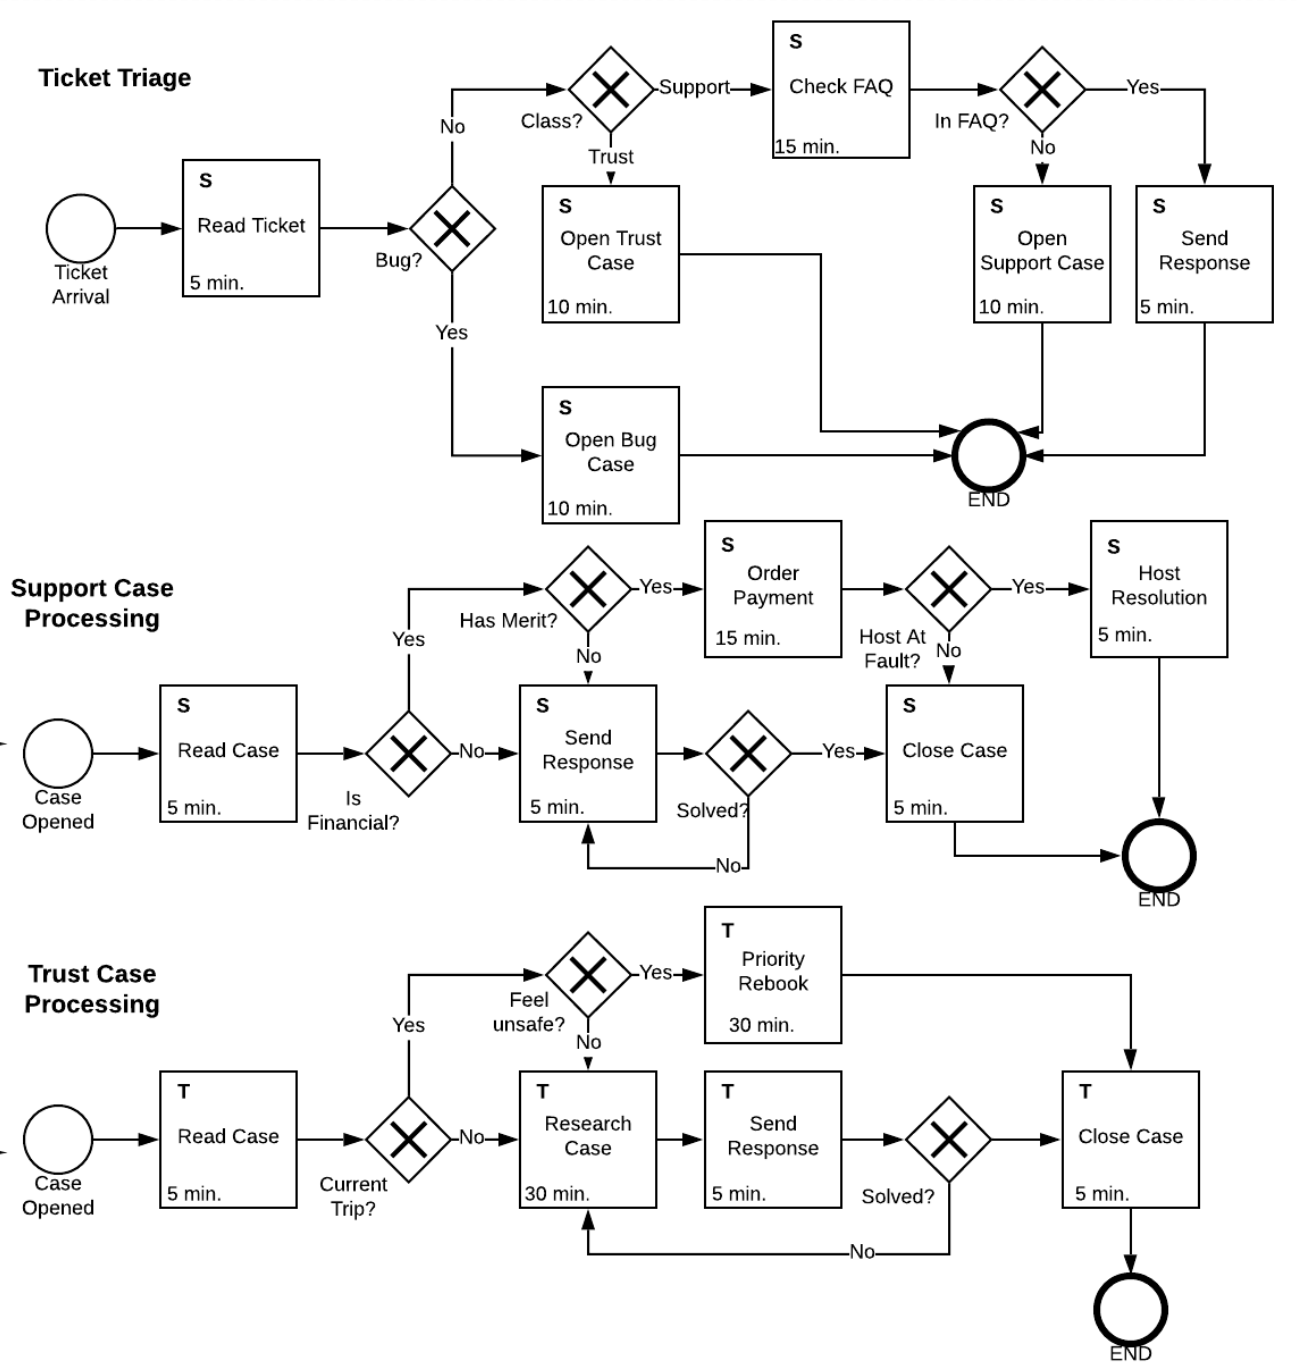
\includegraphics[width=0.8\textwidth]{tex/workflows.png}
  \caption{Customer support workflows, enacted to generate logs}
  \label{fig:workflows}
\end{figure}

\begin{figure}[h!]
  \centering
  \begin{footnotesize}
  \begin{tabular}{|c|c|c|l|l|}\hline
batch               & timestamp     & enactment id  & event type                    & event data                              \\\hline
\multirow{10}{*}{42} & 42             & $\mu_{1}$     & \texttt{ReadCase}            & \{ name=Alice, support=1 \}             \\\cline{2-5}
                    & 42             & $\mu_{1}$     &  \texttt{SendResponse}        & \{ name=Alice \}                        \\\cline{2-5}
                    & 42             & $\mu_{2}$     &  \texttt{ReadCase}            & \{ name=Bob, support=2 \}               \\\cline{2-5}
                    & 42             & $\mu_{1}$     &  \texttt{SendResponse}        & \{ name=Alice \}                        \\\cline{2-5}
                    & 42             & $\mu_{2}$     &  \texttt{SendResponse}        & \{ name=Bob \}                          \\\cline{2-5}
                    & 42             & $\mu_{2}$     &  \texttt{CloseCase}           & \{ name=Bob, support=2 \}               \\\cline{2-5}
                    & 42             & $\mu_{1}$     &  \texttt{CloseCase}           & \{ name=Alice, support=1 \}             \\\cline{2-5}
                    & 42             & $\mu_{3}$     &  \texttt{ReadCase}            & \{ name=David, support=2\}              \\\cline{2-5}
                    & 42             & $\mu_{4}$     &  \texttt{ReadCase}            & \{ name=Charlie, support=1 \}           \\\cline{2-5}
                    & 42             & $\mu_{4}$     &  \texttt{OrderPayment}        & \{ name=Charlie \}                      \\\cline{1-5}
\multirow{3}{*}{43}  & 43             & $\mu_{3}$     &  \texttt{SendResponse}        & \{ name=David \}                        \\\cline{2-5}
                    & 43             & $\mu_{4}$     &  \texttt{SendResponse}        & \{ name=Charlie \}                      \\\cline{2-5}
                    & \dots         & \dots         & \dots                         & \dots                                   \\\hline
    \end{tabular}
  \end{footnotesize}
  \caption{Portion of a log with {\sc support case} enactments with ten events per batch}
  \label{fig:log}
\end{figure}

We generated rules using the workflows' activities, e.g., 
\texttt{ReadCase}, \texttt{SendResponse}, etc.,
and gap atoms with one- to ten-second gaps,
reflecting the typical gaps between events in enactments.
We respect the workflow model's activity ordering
to ensure gap atoms are satisfiable
by some enactments.
We use two classes of rules: ``small'' and ``medium'' rules,
as shown in Figure\:\ref{fig:sample-rules}.
For {\em small} rules,
each rule body has one or two event atoms and no more than one gap,
and each rule head has one event and no more than one gap.
For {\em medium} rules,
each rule body has up to two event atoms and no more than two gaps
and each rule head has up to two event atoms and no more than two gaps.
We also categorize sets of rules by their ``overlap'',
defined in Section\:\ref{subsec:rule-properties}
to approximate the potential for rule interaction.

\begin{figure}[h!]
  \begin{tabular}{lcl}
    \multicolumn{3}{c}{Small rules (2 to 4 atoms), overlap of $0.33$}\\
    $r_1: \texttt{ReadCase}(u,i)@x$                                           & $\rightarrow$ & $\texttt{SendResponse}(u)@y, y {\leq} x + 5$ \\
    $r_2: \texttt{ReadCase}(u,i)@x, \texttt{SendResponse}(u)@y,$              & $\rightarrow$ & $x+10 {\leq} y$ \\
    $r_3: \texttt{ReadCase}(u,i)@x, \texttt{OrderPayment}(u)@y,$              & $\rightarrow$ & $y {\leq} x + 3, \texttt{CloseCase}(u,i)@z$ \\
    \multicolumn{3}{c}{}\\
    \multicolumn{3}{c}{Medium rules (5 to 7 atoms), overlap of $0.66$}\\
    $r_4: \texttt{ReadCase}(u,i)@x$                                             & $\rightarrow$ & $\texttt{SendResponse}(u)@y, x + 3 \leq y$ \\
                                                                                &               & $\texttt{CloseCase}(u,i)@z, z {\leq} x + 5, z {\leq} y + 1$ \\
    $r_5: \texttt{ReadCase}(u,i)@x, \texttt{SendResponse}(u)@y,$   & $\rightarrow$ & $\texttt{CloseCase}(u,i)@z, z {\leq} x + 5, z {\leq} y + 1$ \\
    \hspace{0.5cm}$x + 4 {\leq} y$                                 &               & \\
    $r_6: \texttt{ReadCase}(u,i)@x, \texttt{OrderPayment}(u)@y,$  & $\rightarrow$ & $\texttt{HostResolution}(u)@w, x + 10 {\leq} w$\\
    \hspace{0.5cm}$x + 10 \leq y$                                 &              & $y {\leq} w + 10$ \\ 
  \end{tabular}
  \caption{Sample small and medium-sized rules}
  \label{fig:sample-rules}
\end{figure}

Experiments were run on a single machine:
a desktop Fedora 20 (Linux) machine
with a 2K MHz, 8-core AMD EPYC 7702 processor with 8GB memory.
The implementation was written in Python 3.9.6.
We used the Z3 SMT solver \cite{de2008z3} for satisfiability checking
and the Python bindings for Z3 \cite{z3py}.
Notably,
in early implementations of the monitor,
we invoked the Z3 library many times to instantiate each subformula,
then combined these subformula for the satisfiability test
with z3.Solver.check.
The multiple library calls resulted in much slower processing,
up to $100$ times as long as our reported results;
a frugal use of the solver is critical
to achieve reasonable performance.
The source code of the monitor
and experimental framework is available on Github
\cite{mackeymultirulemonitor}.

\subsection{Detection Often Occurs Far Before Enactments End}
\label{subsec:earliness}

First, we examine how early
violations are detected
with respect to enactments' events.
The quantification of earliness
indicates potential benefits
where the earliness affects the system's response.
For example,
the system may choose to halt an enactment
when a violation is detected,
allowing the system to reclaim resources
or to prevent further policy violations.
We report the average earliness of violation detection
for the single-rule monitor
with respect to the enactment's length.
Because the multi-rule monitoring algorithm
is an extension of the single-rule algorithm
and can detect some violations earlier,
the earliness afforded by multi-rule monitoring
is at least as good as that of single-rule monitoring
and may be better in some cases.

We apply the single-rule monitor
to logs with normal-length ($\approx$10 events)
and large enactments ($\approx$100 events).
For each enactment, we count the observed events after the first
detected violation.
Fig.\,\ref{fig:eval_early_detection_benefits} shows that,
on average, violations are detected at 75\% of
event arrival for normal-length enactments and 34\% for large ones.
As detailed in Section \ref{sec:motiv},
this happens when expected head event atoms are pending,
but their timestamps are bounded by body event atoms
and some gap atoms.
Often,
the upper bound timestamp of a head event atom falls within the enactment's duration,
leading {\sf Detect} to recognize its occurrence in real-time.
We focus on average earliness for single-rule monitoring,
but the multi-rule approach often detects even earlier,
as shown in Section\:\ref{sec:multiple}.
Finally, we note that the average earliness
is affected by the gaps in gap atoms;
more study is needed to understand the relationship
between gap size and average earliness. 

\begin{figure}[ht]
  \vspace{-2mm}
  \centering
  \begin{footnotesize}
    \renewcommand{\arraystretch}{1.6}
  \begin{tabular}[t]{|c||c|c||c|c|}\cline{2-5}
   \multicolumn{1}{c}{}         & \multicolumn{2}{|c||}{\bf Normal-length enactments}          & \multicolumn{2}{|c|}{\bf Large enactments}  \\\hline
    {\bf Rule Size}   & \% events before first violation  & \% after & \% events before first violation  & \% after \\\hline
    {\bf Small}  & 74.9 & 25.1  & 33.5 & 66.5                 \\\hline
    {\bf Medium} & 83.7 & 16.3  & 69.4 & 30.6              \\\hline
  \end{tabular}
  \end{footnotesize}
  \caption{Percentages of events observed before and after the first detected violation}
  \vspace*{-2mm}
  \label{fig:eval_early_detection_benefits}
\end{figure}

\subsection{Detection is Feasible for Medium-scale Applications}
\label{subsec:log-properties}

Next,
we study the feasibility of monitoring.
We evaluate when the monitor
processes batches
in an average of less than one second,
the batch arrival rate.
The batch size and the enactment concurrency
determine the number of assignments
that must be joined and matched
in the {\sf Update} and {\sf Update-E} algorithms,
the number of expected events generated by the {\sf Chase} algorithm,
and the number of matches that contribute 
to the formula produced by {\sf Build},
so we expect that increasing these parameters raises the processing time.

First, we report the average processing time
for the single-rule monitor (Section \ref{sec:alg})
in Figure\:\ref{fig:eval_avg_proc_time}.
The average processing time is far less than one second
for all batch sizes and enactment lengths,
shorter than $0.07$ seconds for all small rules and 
shorter than $0.2$ seconds for all medium rules,
indicating that the single-rule monitor is feasible
for logs with those properties.
These times increase linearly with the batch size,
which is expected for small rules,
as the number of possible assignments
does not yet suffer the combinatorial explosion.
For medium rules, however,
the average processing time also increases linearly
with the batch size;
this is unexpected because
to make the number of assignments
is exponential in the batch size.
This may be due to the increasing number of gap atoms,
as more gap atoms decrease
the number of assignments in the body or head table.
This phenomenon requires a more thorough investigation
of the effects of gap atoms on the assignment database.

\begin{figure}[ht]
  {
    \centering
    \begin{footnotesize}
      \renewcommand{\arraystretch}{1.6}
    \begin{tabular}[t]{|c||c|c||c|c||}\cline{2-5}
    \multicolumn{1}{c}{}& \multicolumn{4}{|c|}{\bf Enactment Length}\\\cline{2-5}
    \multicolumn{1}{c}{} & \multicolumn{1}{|c|}{\bf Normal}
    & \multicolumn{1}{|c||}{\bf Large} 
    & \multicolumn{1}{|c|}{\bf Normal}
    & \multicolumn{1}{|c|}{\bf Large} \\\hline
    {\bf Batch Size} & \multicolumn{2}{|c||}{{\bf Small Rules}} & \multicolumn{2}{|c||}{{\bf Medium Rules}}\\\hline\hline
    100             & 4.55$\times10^{-4}$     & 6.19$\times10^{-4}$     & 7.74$\times10^{-4}$     & 1.363$\times10^{-3}$     \\\hline
    1,000           & 4.330$\times10^{-3}$    & 6.177$\times10^{-3}$    & 7.534$\times10^{-3}$    & 1.3509$\times10^{-2}$     \\\hline
    10,000          & 4.2414$\times10^{-2}$   & 6.0769$\times10^{-2}$   & 7.4925$\times10^{-2}$   & 1.35218$\times10^{-1}$     \\\hline
    \end{tabular}
  \end{footnotesize}
    \vspace*{-2mm}
    \caption{Batch Processing Times (seconds) by Batch Size, Rule Size, and Enactment Length}
    \label{fig:eval_avg_proc_time}
    }
  \end{figure}

We also evaluated the feasibility of the multiple-rule monitor.
We monitored logs with normal-length enactments
and rule sets with three medium rules
with an average overlap of one event atom.
The results in Table \ref{tab:experiment-log-properties} show
the batch processing time increases with the batch size and concurrency
as expected.
Second,
the average processing time is ${\le}1$ second
for batches of $100$ events and an average enactment concurrency of $100$.
Beyond these values,
the average processing time exceeds ${\ge}1$ second,
shown by parentheses in the table,
but is still ${\le}10$ seconds.

We note here that 
our experiments were conducted on a single commodity machine
rather than enterprise-grade hardware;
our results suggest that
multi-rule monitoring would be feasible
for a wider range of applications,
i.e., larger batches and more concurrent enactments,
if the monitoring is performed with more powerful hardware resources.

\begin{table}[htbp]
    \centering
    \begin{footnotesize}
  \begin{tabular}{|c|c|c|c|c|c|}
  \hline
  \textbf{Batch Size} & \textbf{Conc=10} & \textbf{Conc=50} & \textbf{Conc=100}  & \textbf{Conc=500}  & \textbf{Conc=1,000} \\\hline\hline
  10                  & 0.061            & 0.046            & 0.294              & (1.253)              & (3.031)               \\\hline
  50                  & 0.195            & 0.169            & 0.403              & (2.506)              & (3.269)               \\\hline
  100                 & 0.374            & 0.328            & 0.553              & (2.807)              & (3.483)               \\\hline
  500                 & (1.256)          & (1.851)          & (1.326)            & (3.347)              & (5.279)               \\\hline
  \hline
  \end{tabular}
\end{footnotesize}
  \caption{Average Batch Processing Time (seconds) by Batch Size and Concurrency}
  \label{tab:experiment-log-properties}
\end{table}

\subsection{Detection Remains Feasible for Complex Sets of Rules}
\label{subsec:rule-properties}

Another factor affecting the feasibility of monitoring
is the size and ``overlap'' the sets of rules.
The {\em overlap} for a set of rules
is the number of pairs of event atoms
that share the same name
such that one appears in the head of one rule
and the other appears in the body of another rule,
divided by the total number of rule pairs.
More overlap between rules increases the number of assignments
generated by expected events from the {\sf Chase} algorithm,
thus increasing the number of assignments to process into
the assignment database by {\sf Update} and {\sf Update-E}.
Furthermore,
expected events can create more expected events
in the subsequent executions of the {\sf Chase} algorithm's
{\bf while} loop,
but this feedback is ultimately limited by the acyclicity
of the rule set.
Finally,
expected events carry marked nulls,
which are added to the formula produced by {\sf Build},
so more overlap grows the subformula in the formula
that share variables;
this may increase the time to check its satisfiability.

We used logs with batches of one hundred events
and an average of one hundred concurrent enactments,
as these values were found to be within the feasible range
for the multi-rule monitor
in Section\:\ref{subsec:log-properties}.
We generated thirty sets
with two to four small rules,
calculating the overlap by summing the overlap
for each pair of rules,
then dividing by the number of rule pairs.
We place each rule in one of five categories:
$0.33$, $0.66$, $1$, $1.33$, and $1.66$ event atoms,
whichever is closest to its average overlap.
In Table\:\ref{tab:overlap-experiment}, 
we report the average batch processing time
with any time above the batch arrival rate of one second
shown in parentheses to indicate infeasibility.
the overlap grows exponential as the overlap increases linearly.
Furthermore,
we see when the average overlap
exceeds $1$ event atom per rule pair,
the processing time exceeds one second,
the threshold for feasibility.

\begin{table}[htbp]
  \centering
\begin{tabular}{|c|c|c|c|c|}
\hline
\textbf{Overlap$\approx$0.33}  & \textbf{Overlap$\approx$0.66} & \textbf{Overlap$\approx$1} & \textbf{Overlap$\approx$1.33} & \textbf{Overlap$\approx$1.66} \\\hline\hline
0.048                  & 0.169                 & 0.356              & (1.22)                  & (3.17)                  \\\hline
\end{tabular}
\caption{Average Batch Processing Time (seconds) by Average Overlap}
\label{tab:overlap-experiment}
\end{table}

We also evaluated the effect of varying the number of rules
while keeping a constant overlap.
More rules grows the number of tables and entries
in the assignment databases,
as well as the number of expected events
generated by the {\sf Chase},
as each rule's body assignment generates expected events.
The average overlap for the sets of rules was $0.54$,
so we used five rule sets of two, three, four, and five small rules
with an overlap of $0.54 \pm 0.2$.
We report the average batch processing times
in Table\:\ref{tab:number-rules-experiment}.
The batch processing time increases
exponentially with the number of rules;
this suggests the number of rules
is similarly critical to the feasibility of monitoring
as the overlap,
where rule sets with relatively low overlap
can become infeasible
when the number of rules exceeds four.

\begin{table}[htbp]
  \centering
\begin{tabular}{|c|c|c|c|}
\hline
\textbf{2 rules} & \textbf{3 rules} & \textbf{4 rules} & \textbf{5 rules} \\\hline\hline
0.014                  & 0.099      & 0.395            & (1.582)            \\\hline
\end{tabular}
\caption{Average Batch Processing Time (seconds) for Overlap${\approx}0.54$ by Number of Rules}
\label{tab:number-rules-experiment}
\end{table}

In summary, our evaluation
quantifies
the benefits of early violation detection
and the feasibility of monitoring
with respect to the size and complexity of logs and rules.
We identify the algorithms and subroutines 
that are most affected by these dimensions
and provide explanations for the observed trends.
We also identify dimensions of logs and rules
that deserve further investigation,
such as the effects of gap size on earliness
and the effects of gap size and number of gaps on processing time.
Finally,
we note that these findings are limited 
to applications with similar characteristics as the sample logs
and rules we used in our evaluation,
and thus may not generalize to arbitrary event-based systems.
More work is needed to extend these findings to a wider range of applications,
particularly by testing real-world logs and rules.

\section{Related Work}
\label{sec:early-violation-detection-related-work}

We first discuss related work that reasons algorithmically
about when a violation is inevitable.
Then, we compare our work with other approaches
that monitor constraints with data values.

A key technique in this work
is to detect violations at the earliest possible time.
References \cite{maggi2011monitoringcolored,maggi2012runtime,
maggi2011runtime} studies violations
of constraints in {\sc declare} language,
using
an encoding of violations' temporary or permanent status in states of automata.
Quantitative time constraints,
such as ``for every request followed within five days by a response,
a payment is made within three days of the response and three days of the request'',
are important
for applications of runtime monitoring \cite{ly2015compliance},
but difficult to encode in automata,
as evidenced by the previous chapter.
We identify violations
as inevitable or not
by partially instantiating constraints
with observed timestamps and data values
and checking satisfiability of the resulting constraints.
References \cite{dousson2007chronicle} and \cite{maggi2019compliance}
also partially initialize
constraints to detect violations,
but do not consider interactions between sets of constraints,
which may produce earlier violations as illustrated above.

Another functionality of runtime constraints
considered by this chapter
is the comparison of data values,
such as matching the user who makes a request
to the user who receives a response.
References \cite{de2013runtime,riccardo2014monitoringfsa}
monitor constraints in first-order LTL
with automata whose states have relational data stores,
though they assume a fixed, finite domain of data values,
which is impractical for large applications.
Quantified event automata, finite-state automata
with transitions labeled by quantified first-order formulas,
can also monitor data-dependent constraints
\cite{barringer2012quantified}.
Their approach creates and manages bindings to variables,
but is limited by the same drawbacks as
automata-based approaches described above.
Other work on first-order LTL uses exclusively relational data structures
as auxillary storage for violation detection
\cite{Chomicki95:TODS,halle2012runtime,basin2015monitoring,havelund2018efficient},
though they do not calculate deadlines explicitly
because they do not use quantitative time constraints.
Also relevant is the technique of trace slicing
\cite{chen2009parametric},
filtering an enactment
into disjoint enactments with related data,
allowing multiple monitors to run in parallel.
Our work does not use trace slicing,
but it seems promising for optimization
as a pre-processing step
to parallelize our approach.

% References \cite{, cimatti2020smt, havelund2018efficient, calvanese2022verification}

Other relevant data-centric approaches
are those for relational databases and Datalog rules.
Incremental view maintenance
for Datalog provides incremental algorithms
for updating the results of views or queries
when the underlying database changes;
\cite{gupta1993maintaining} maintains
Datalog and SQL views
without gap constraints
nor existential variables and multiple atoms in the rule head.
A key technique in this work comes from the observation that
because we use Datalog-like rules,
the possibility of rules triggering other rules
can be simulated by the chase \cite{AHV95},
which we adapt for our setting in Section\:\ref{sec:multiple}.
Other work on the chase
for Datalog with arithmetic constraints
targets problems that don't apply to our setting
of monitoring an enactment at runtime,
including computing certain query answers \cite{afrati2008data, ten2013data}.

\section{Chapter Summary}
\label{sec:rules-data-conclusion}

This chapter presents techniques for detecting violations
of individual rules and sets of rules with data,
extending the class of rules that can be monitored.
We showed that detecting violations at the earliest possible time.
can be accomplished by reasoning about timestamps,
simulating rule interaction,
and applying satisfiability testing to potential violations.
We also conducted an empirical evaluation of our techniques
to show that they are effective and efficient
for small- and medium-sized batches
and rules,
though more study is needed
to determine their effectiveness and efficiency
with enterprise-scale computing resources.
In the next chapter,
we explore the use of aggregation functions
over time windows in rules.
\chapter{Rules with Aggregation}
\label{chapter:aggregation}

This chapter studies
for rules with aggregation functions.
The high volume of data and relatedness of events in enactments
encourages specification that aggregate properties of groups of data.
For example,
a banking application may report an account is suspicious for money laundering
if the sum of the account's payments in a 24-hour period exceeds \$50,000,
even if no individual transaction exceeds that amount.
Such rules
call for monitoring techniques
that use aggregation functions.
These functions
introduces new challenges
of reasoning about functions on multiple events,
as well as numeric data.
In this chapter, we develop a syntax and semantics
for extending our rules with aggregation functions.
Then,
we provide two ways of addressing the challenges
of early violation detection.
The first is to rewrite aggregation
with Datalog$_{\mathbb{Z}}$ programs,
which allows us to use the results of the previous chapter
with minimal changes.
The second is to adapt the chase process
to reason with aggregation functions.

This chapter is organized as follows:
in Section \ref{section:aggregation-definitions},
we add time windows and aggregation functions over these windows
to rule syntax and semantics.
In Section \ref{section:aggregation-datalog-program},
we provide Datalog$_{\mathbb{Z}}$ programs that generate events
with the results of aggregation
without calling the underlying aggregation functions directly.
In Section \ref{section:chasing-rules-with-aggregation},
we combine the algorithms from the previous chapter 
to perform early violation detection,
by adapting the chase process
and rewriting aggregation functions in Presburger arithmetic (PA).
Finally,
in Sections\:\ref{section:aggregation-related-work} and \ref{section:aggregation-summary}
discuss related work and conclude the chapter.

\section{Time Windows for Aggregation Functions}
\label{section:aggregation-definitions}

Now, we present the syntax for rules with aggregation,
which uses different types of windows
to collect events
and five aggregation functions
to aggregate the values of events in a window.
Then,
we describe the semantics of rules with aggregation,
which do not just constrain event, but also generate events
that hold the results of applying aggregation functions.
Finally,
we describe an assumption about target enactments
we make to simplify the problem
and a preprocessing step
that enables this assumption.
The results in the remainder of this chapter
assume that the workflow assumption holds.

\begin{examp}\label{examp:banking-aggregation-rules}
We illustrate the aggregation model with
a banking application
where users deposit money into their accounts.
Enactments for this application include
events for users' deposits
and bankers' approval of users' activity,
with two event types:
{\tt Deposit},
with {\em user} and {\em amount} attributes,
and {\tt Approve}, with the {\em user} attribute.
The {\em user} values come from the data domain $\Dom$
and {\em amount} values are positive integers in $\mathbb{N}$.

Consider if the bank
requires that over every three-day period:
($1$) the sum of deposits must be at most $\$20$ and
($2$) some deposit is more than $\$10$.
These requirements are
specified by the rules $r_1$ and $r_2$, respectively,
in Figure~\ref{fig:aggregation-rules-2}.
Rule $r_1$ 
computes the sum of all deposits for a user
over each three-day window
in a new ``aggregation event'' type
$\mbox{\tt SumDep}(\mbox{\em{sum}},\mbox{\em start})$.
This event type has two attributes:
{\em sum} is the sum of the deposits in the window
and {\em start} is the first timestamp of the window.
The gap atom $a'\leq 20$ in the rule head
requires that the sum $a'$ is at least $\$20$.
Rule $r_2$ aggregates
the maximum deposit for a user
over each three-batch window
in a new aggregation event type
$\mbox{\tt MaxDep}(\mbox{\em max},\mbox{\em start})$,
where {\sc max} is the maximum of the deposits in the window
and {\em start} is the first timestamp of the window.
The gap atom $b'\geq 10$ in the rule head
enforces the requirement that the maximum $b'$ is at least $\$10$.
\end{examp}

\begin{figure}[ht]
    \centering
\begin{tabular}{lcl}
$r_1: \mbox{\tt SumDep}(u,a'=\mbox{\sc sum}(a),s)@(s+3)$, $a'\leq 20$ & $\leftarrow$ & {\sc tumbling}$(s,s+3)$                \\
                                                                    &                & {\sc from} \mbox{\tt Deposit}$(u,a)@z$   \\
                                                                    &                &                                          \\
$r_2: \mbox{\tt MaxDep}(u,b'=\mbox{\sc max}(b),s)@(s+3)$, $b'\geq 10$ & $\leftarrow$ & {\sc tumbling}(s,s+3)                  \\
                                                                    &                & {\sc from} \mbox{\tt Deposit}$(u,b)@z$   \\
                                                                    &                &                                          \\
\end{tabular}
\caption{Two rules $r_1$ and $r_2$ with aggregation functions over two types of sliding windows}
\label{fig:aggregation-rules-2}
\end{figure}

The rule heads contain atoms
that name events that hold the results of aggregation functions
and additionally may gap atoms on those events.
We allow the aggregation functions
sum ({\sc sum}),
maximum ({\sc max}),
minimum ({\sc min}),
count ({\sc count}),
and
count-unique ({\sc countu}).
The values $-\infty$ and $\infty$
are the default values for {\sc max} and {\sc min}, respectively;
we assume these values not present in the enactment
and
are used when the window contains no events.
The value $0\in\N$ is the default value for {\sc sum},
{\sc count}, and {\sc countu}.

The {\em window expression},
e.g.,
{\sc tumbling}$(s,s+3)$ in $r_1$,
indicates which events are collected in windows for $r_1$.
We use two classes of windows,
either {\em moving} or {\em triggered},
which are defined by the window expression.
Moving windows are either
{\em sliding} and {\em tumbling} windows;
they have a constant length and
are evaluated at every timestamp
or at every timestamp that is a multiple of the window length, respectively,
regardless of the enactment's events.
The {\em sliding} window
is parametrized by its window length $L$ for some $L\geq 1$;
it generates a window for the interval of timestamps $[1,L]$,
and then, for each integer $i$, the interval $i$ through $i+L$,
assuming the enactment extends to $i+L$.
The {\em tumbling} window
is defined by a window length $L$, and
includes the window $[1,L]$,
then the window $[kL+1,kL+L]$ for every integer $k\geq 1$.
Fig.\:\ref{fig:moving-windows} shows an example of moving windows.
On the top of the figure,
{\tt Deposit} source events appear at each timestamp.
Sliding and tumbling windows are shown as boxes of length $3$,
with the window's aggregation event inside the box.

\begin{figure}[ht]
\centering
\begin{tikzpicture}[node distance=0.3cm,>=stealth',bend angle=45,auto]
    \begin{small}
        
% Deposit events
\node[rectangle, rounded corners, draw, text width=1.2cm, align=center, minimum height=0.5cm] (event1) {D(40)@1};
\node[rectangle, rounded corners, draw, text width=1.2cm, align=center, minimum height=0.5cm, right=of event1] (event2) {D(10)@2};
\node[rectangle, rounded corners, draw, text width=1.2cm, align=center, minimum height=0.5cm, right=of event2] (event3) {D(10)@3};
\node[rectangle, rounded corners, draw, text width=1.2cm, align=center, minimum height=0.5cm, right=of event3] (event4) {D(0)@4};
\node[rectangle, rounded corners, draw, text width=1.2cm, align=center, minimum height=0.5cm, right=of event4] (event5) {D(0)@5};
\node[rectangle, rounded corners, draw, text width=1.2cm, align=center, minimum height=0.5cm, right=of event5] (event6) {D(15)@6};
\node[rectangle, rounded corners, draw, text width=1.2cm, align=center, minimum height=0.5cm, right=of event6] (event7) {D(20)@7};
\node[rectangle, rounded corners, draw, text width=1.2cm, align=center, minimum height=0.5cm, right=of event7] (event8) {D(5)@8};
\node[rectangle, rounded corners, draw, text width=1.2cm, align=center, minimum height=0.5cm, right=of event8] (event9) {D(0)@9};

% Arrows for chain of events
\draw[-] (event1.east) to [out=0,in=180] (event2.west);
\draw[-] (event2.east) to [out=0,in=180] (event3.west);
\draw[-] (event3.east) to [out=0,in=180] (event4.west);
\draw[-] (event4.east) to [out=0,in=180] (event5.west);
\draw[-] (event5.east) to [out=0,in=180] (event6.west);
\draw[-] (event6.east) to [out=0,in=180] (event7.west);
\draw[-] (event7.east) to [out=0,in=180] (event8.west);
\draw[-] (event8.east) to [out=0,in=180] (event9.west);

% Tumbling Windows
\node[rectangle, draw, text width=4.8cm, minimum height=0.5cm, below=of event2] (twindow1) {{\tt TumblingSum}(60, 1)@3};
\node[rectangle, draw, text width=4.8cm, minimum height=0.5cm, below=of event5] (twindow2) {{\tt TumblingSum}(15, 3)@5};
\node[rectangle, draw, text width=4.8cm, minimum height=0.5cm, below=of event8] (twindow3) {{\tt TumblingSum}(25, 5)@7};

% Sliding Windows
\node[rectangle, draw, text width=4.8cm, minimum height=0.5cm, below=of twindow1, node distance=1cm] (slidewindow1) {{\tt SlidingSum}(60, 1)@3};
\node[rectangle, draw, text width=4.8cm, minimum height=0.5cm, right of=slidewindow1, below=of slidewindow1, xshift=1.5cm, yshift=0.0cm] (slidewindow2) {{\tt SlidingSum}(20, 2)@4};
\node[rectangle, draw, text width=4.8cm, minimum height=0.5cm, right of=slidewindow2, below=of slidewindow2, xshift=1.4cm, yshift=0.0cm] (slidewindow3) {{\tt SlidingSum}(10, 3)@5};
\node[rectangle, draw, text width=4.8cm, minimum height=0.5cm, right of=slidewindow3, below=of slidewindow3, xshift=1.4cm, yshift=0.0cm] (slidewindow4) {{\tt SlidingSum}(15, 4)@6};

% Vertical lines
% \draw[dashed] (event1.west) to (slidewindow1.west);
% \draw[dashed] (event2.west) to (slidewindow2.west);
% \draw[dashed] (event3.west) to (slidewindow3.west);
% \draw[dashed] (event4.west) to (slidewindow4.west);
% \draw[dashed] (event7.west) to (twindow3.west);

\end{small}
\end{tikzpicture}
\caption{An enacment with {\tt Deposit} ({\tt D}) events, tumbling and sliding windows for window length $3$, and aggregation events {\tt TumblingSum} and {\tt SlidingSum}}
\label{fig:moving-windows}
\end{figure}

The second class of windows
are those with event triggers.
For a {\em start-triggered} window of length $L$,
a window $[s,s+L]$ is generated
whenever a specified event occurs at time $s$.
Similarly, for an {\em end-triggered} window,
a window $[e-L,e]$ is generated
whenever a specified event occurs at time $e$.
Finally,
a {\em start-end-triggered} window
indicates a window between every pair of
start and end events.
Consider the enactment and corresponding windows
in Figure~\ref{fig:triggered-windows}.
The start trigger {\tt B}
and
the end trigger {\tt C} events
are shown above the {\tt Deposit} source events.
Windows are shown as boxes, 
with vertical, dashed Lines
matching each window to its start and end events.

\begin{figure}[ht]
\centering
\begin{tikzpicture}[node distance=0.5cm,>=stealth',bend angle=45,auto]
\begin{small}
\node[rectangle, rounded corners, draw, text width=1.1cm, align=center, minimum height=0.5cm] (event1) {D(5)@1};
\node[rectangle, rounded corners, draw, text width=1.1cm, align=center, minimum height=0.5cm, right=of event1] (event2) {D(5)@2};
\node[rectangle, rounded corners, draw, text width=1.1cm, align=center, minimum height=0.5cm, right=of event2] (event3) {D(1)@3};
\node[rectangle, rounded corners, draw, text width=1.1cm, align=center, minimum height=0.5cm, right=of event3] (event4) {D(0)@4};
\node[rectangle, rounded corners, draw, text width=1.1cm, align=center, minimum height=0.5cm, right=of event4] (event5) {D(0)@5};
\node[rectangle, rounded corners, draw, text width=1.1cm, align=center, minimum height=0.5cm, right=of event5] (event6) {D(5)@6};
\node[rectangle, rounded corners, draw, text width=1.1cm, align=center, minimum height=0.5cm, right=of event6] (event7) {D(2)@7};
\node[rectangle, rounded corners, draw, text width=1.1cm, align=center, minimum height=0.5cm, right=of event7] (event8) {D(5)@8};

% Events
\node[rectangle, rounded corners, draw, text width=1.1cm, align=center, minimum height=0.5cm, above=of event1] (bevent1) {B@1};
\node[rectangle, rounded corners, draw, text width=1.1cm, align=center, minimum height=0.5cm, right=of bevent1] (bevent2) {B@2};
\node[rectangle, rounded corners, draw, text width=1.1cm, align=center, minimum height=0.5cm, above=of event5] (bevent5) {C@5};
\node[rectangle, rounded corners, draw, text width=1.1cm, align=center, minimum height=0.5cm, above=of event6] (bevent6) {B@6};
\node[rectangle, rounded corners, draw, text width=1.1cm, align=center, minimum height=0.5cm, above=of event8] (bevent8) {C@8};

% Lines for events
\draw[-] (bevent1.east) to [out=0,in=180] (bevent2.west);
\draw[-] (bevent2.east) to [out=0,in=180] (bevent5.west);
\draw[-] (bevent5.east) to [out=0,in=180] (bevent6.west);
\draw[-] (bevent6.east) to [out=0,in=180] (bevent8.west);

% Arrows for chain of events
\draw[-] (event1.east) to [out=0,in=180] (event2.west);
\draw[-] (event2.east) to [out=0,in=180] (event3.west);
\draw[-] (event3.east) to [out=0,in=180] (event4.west);
\draw[-] (event4.east) to [out=0,in=180] (event5.west);
\draw[-] (event5.east) to [out=0,in=180] (event6.west);
\draw[-] (event6.east) to [out=0,in=180] (event7.west);
\draw[-] (event7.east) to [out=0,in=180] (event8.west);

% Start-triggered windows
\node[rectangle, draw, text width=4.8cm, minimum height=0.5cm, below=of event2, xshift=0cm] (startwindow1) {{\tt BStart-Sum}(11,1)@3};
\node[rectangle, draw, text width=4.8cm, minimum height=0.5cm, below=of event2, xshift=1.8cm, yshift=-0.6cm] (startwindow2) {{\tt BStart-Sum}(6,2)@4};
\node[rectangle, draw, text width=4.8cm, minimum height=0.5cm, below=of event6, xshift=1.8cm] (startwindow3) {{\tt BStart-Sum}(12,6)@8};

% End-triggered windows
\node[rectangle, draw, text width=4.8cm, minimum height=0.5cm, below=of event3, xshift=1.8cm, yshift=-1.4cm] (endwindow1) {{\tt CEnd-Sum}(1,3)@5};
\node[rectangle, draw, text width=4.8cm, minimum height=0.5cm, below=of event6, xshift=1.8cm, yshift=-1.4cm] (endwindow2) {{\tt CEnd-Sum}(12,6)@8};

%Start-End-triggered window
\node[rectangle, draw, text width=8.3cm, minimum height=0.5cm, below=of event2, xshift=1.9cm, yshift=-2.4cm] (startendwindow3) {{\tt BStart-CEnd-Sum}(11,1)@5};
\node[rectangle, draw, text width=6.5cm, minimum height=0.5cm, below=of event2, xshift=2.8cm, yshift=-3.0cm] (startendwindow4) {{\tt BStart-CEnd-Sum}(6,2)@5};
\node[rectangle, draw, text width=13.8cm, minimum height=0.5cm, below=of event2, xshift=4.6cm, yshift=-3.6cm] (startendwindow3) {{\tt BStart-CEnd-Sum}(24,1)@8};
\node[rectangle, draw, text width=12.0cm, minimum height=0.5cm, below=of event2, xshift=5.5cm, yshift=-4.2cm] (startendwindow4) {{\tt BStart-CEnd-Sum}(12,2)@8};
\node[rectangle, draw, text width=4.8cm, minimum height=0.5cm, below=of event6, xshift=1.8cm, yshift=-4.8cm] (startwindow3) {{\tt BStart-CEnd-Sum}(12,6)@8};

% Vertical lines for End-triggered windows
% \draw[dashed] (bevent5.east) to (endwindow1.east);

% Vertical lines for start-end-triggered windows
% \draw[dashed] (bevent6.west) to (startendwindow2.west);
% \draw[dashed] (bevent8.east) to (startendwindow2.east);

% Vertical lines for start-end-triggered windows
% \draw[dashed] (bevent2.south west) -- ($(bevent2.south west)+(270:1.5cm)$);
% \draw[dashed] (startwindow2.south west) to (startendwindow1.north west);
% \draw[dashed] (bevent5.east) to (startendwindow1.east);

% Vertical lines for start-triggered windows
% \draw[dashed] (bevent1.west) to (startwindow1.west);
\end{small}
\end{tikzpicture}

\caption{Triggered windows, triggered by start event {\tt B} and end event {\tt C}}
\label{fig:triggered-windows}
\end{figure}

The rule semantics for aggregation expressions
are different from the semantics for non-aggregation expressions:
rules with aggregation generate ``aggregation events''.
To define these semantics,
we refine the event model
to distinguish between {\em external} or {\em internal} events.
External events are generated by an outside source;
this is the event model in the previous chapters.
Internal events are generated by the monitoring system,
here for each window of an aggregation rule.
For an enactment $\eta$ and an aggregation rule $r$,
for each window $W$ defined by the window expression in $\mbox{\em body}(r)$,
an internal {\em aggregation event} is generated
with the timestamp of the last event in $W$
and the value of the aggregation function in $\mbox{\em head}(r)$
applied to data values for the attribute
and source events in $W$ designated by the rule body.

This new presence of aggreagtion functions
require reasoning about collections of events,
including overlapping windows.
Furthermore,
the results of aggregation functions
are numeric values;
previously we only needed to reason about data values in $\Dom$
and timestamps.
This motivates the development of extension of the chase process
and satisfiability checking
to rules with aggregation functions.
Thus, the technical problem addressed by this chapter is:
given a set of rules
with aggregation functions,
report an enactment's violations
at the earliest possible time.

As a simplifying assumption,
we assume that for each event type
that acts as a source for an aggregation rule,
there is exactly one event of that type per timestamp.
We call this the {\em workflow assumption},
also referred to as the {\sc declare} assumption in \cite{de2014reasoning}
and the {\em simplicity} assumption in \cite{chiariello2023ltl}.
This assumption limits the types of enactments
to which our results apply,
but it is needed for the correctness of the Datalog$_{\mathbb{Z}}$ programs
in the algorithms in the following section.
Additionally,
we use a preprocessing step that modifies an input enactment
with {\em at most one} event per type per timestamp
to produce an enactment where each event type has {\em exactly one} event per timestamp.
This preprocessing step
adds an attribute {\em real} to each event type.
If an event of that type at a timestamp is present in the input enactment,
{\em real} is set to $1$.
Otherwise,
a placeholder event is added with the value $0$ for {\em real}
and $0$ for all other attributes.
We give an example of this preprocessing in Fig.\:\ref{fig:preprocessing-example}.
Our results in the remainder of this chapter
assume that the workflow assumption holds.

\begin{figure}[h!]
  \centering
\begin{tabular}{|c|c|c|}\hline
    timestamp & Source events              & Preprocessed events        \\\hline
    $1$       & \texttt{Deposit}$(10)@1$      & \texttt{Deposit}$(10,1)@1$      \\\hline
    $2$       & \texttt{Deposit}$(40)@2$      & \texttt{Deposit}$(40,1)@2$      \\\hline
    $3$       &                           & \texttt{Deposit}$(0,0)@3$       \\\hline
    $4$       & \texttt{Deposit}$(10)@4$      & \texttt{Deposit}$(10,1)@4$      \\\hline
    $5$       &                           & \texttt{Deposit}$(0,0)@5$       \\\hline
\end{tabular}
\caption{Preprocessing by adding an attribute {\em real} to each event type.}
\label{fig:preprocessing-example}
\end{figure}

\section{Datalog$_{\mathbb{Z}}$ Generation of Aggregation Events}
\label{section:aggregation-datalog-program}

In this section,
we present Datalog$_{\mathbb{Z}}$ programs \cite{dantsin2001complexity}
to generate aggregation events.
This variant of Datalog allows integer constants and arithmetic expressions in the head and body of rules.
For consistency with our language,
we use the same ``@'' syntax for the event's timestamps.
We provide programs for
{\sc max} for sliding, tumbling,
start-triggered, and end-triggered windows;
%and start- and end-triggered window,
{\sc count} for sliding windows,
and
{\sc sum} for sliding windows.
The other functions and window types are handled
with similar programs.
This provides a means of early violation detection
for rules with aggregation functions,
by rewriting rules with aggregation as Datalog$_{\mathbb{Z}}$ programs
and using these programs to generate aggregation events,
then applying the algorithms in the previous chapter without modification.

The structure of the Datalog$_{\mathbb{Z}}$ program
is consistent across the different
types of windows:
some event \texttt{incX}
with an ``accumulator'' attribute
stores the partial result of the aggregation function
over the partial window,
up to the current timestamp.
To compute \texttt{incX},
some rules initialize \texttt{incX}
with the first source event's value,
then other rules propagate \texttt{incX}
with \texttt{incX} from the previous timestamp
and the current source event's value.
Finally,
a rule reports \texttt{resultX}
when the window is complete.
In these programs,
we simplify the presentation
by removing the non-aggregated attributes
from the source ({\tt Src}) events,
and use {\tt V} for the target attribute.

\subsection{Sliding window with {\sc max} function}
\label{sec:sliding-max-datalog-program}

Let \texttt{Src} be the source event and $L+1$
the sliding window size for a rule
with the {\sc max} function,
i.e., the rule has the form of Fig.\:\ref{fig:sliding-max-rule}.

\begin{figure}[h!]
\begin{tabular}{ll}
\texttt{resultSlidingMax}$(\mbox{\sc max}(a),s)@(s+L) \leftarrow$   & $\textsc{Over}\ \mbox{\sc sliding}(s,s+L)$\\
                                                                    & $\textsc{From}\ \mbox{\tt Src}(a)@x$
\end{tabular}
\caption{Rule with the {\sc max} function and a sliding window of size $L+1$.}
\label{fig:sliding-max-rule}
\end{figure}

An internal event \texttt{resultSlidingMax}
is generated for each window,
with attributes {\em value} (the maximum value),
{\em start} and {\em end} (of the window), and {\em time}
(when the result is produced)
for each window $[$\mbox{\em start},
\mbox{\em end}$]$ of length $L+1$.
To compute \texttt{resultSlidingMax} incrementally,
we use an internal event \texttt{incSlidingMax} with attributes
{\em accumulator}, {\em start}, {\em end}, and {\em stop},
where {\em accumulator}
holds the maximum value seen from {\em start} to {\em stop},
and {\em end} attribute is the target window's last timestamp,
i.e., when the result should be reported.
The Datalog$_{\mathbb{Z}}$ program (Fig.\:\ref{fig:sliding-max-program})
initializes \texttt{incSlidingMax} at each timestamp $T$
with the start of a sliding window.
The source event's value is stored in the accumulator
(of $-\infty$ if the source event is not real),
and $T{+}L$ as the window end.
At each timestamp $T$ that is not greater than the window end,
if the source event at $T$ is real,
the accumulator's value at $T$
is compared with the source event's value at $T{+}1$.
Otherwise, the accumulator is passed along.
At the window's end,
the accumulator is reported with \texttt{resultSlidingMax}.

\begin{figure}[h!]
\begin{mdframed}[leftmargin=0pt,rightmargin=0mm]
\begin{small}
\begin{tabular}{ll}
\multicolumn{2}{l}{Initialize \texttt{incSlidingMax}}\\
\texttt{incSlidingMax}$(V, T, T{+}L)@T$ & $\leftarrow \mbox{\tt Src}(V,1)@T$\\
\texttt{incSlidingMax}$(-\infty, T, T{+}L)@T$ & $\leftarrow \mbox{\tt Src}(V,0)@T$\\
& \\
\multicolumn{2}{l}{Propagate \texttt{incSlidingMax}}\\
\texttt{incSlidingMax}$(V, S, E)@(T{+}1)$ & $\leftarrow$ \texttt{incSlidingMax}$(A, S, E)@T ,\  \mbox{\tt Src}(V,1)@(T{+}1) ,\  (A{<}   V),\ (T{+}1 {\leq} E)$\\
\texttt{incSlidingMax}$(A, S, E)@(T{+}1)$ & $\leftarrow$ \texttt{incSlidingMax}$(A, S, E)@T ,\  \mbox{\tt Src}(V,1)@(T{+}1) ,\  (A{\geq}V),\ (T{+}1 {\leq} E)$\\
\texttt{incSlidingMax}$(A, S, E)@(T{+}1)$ & $\leftarrow$ \texttt{incSlidingMax}$(A, S, E)@T ,\  \mbox{\tt Src}(V,0)@(T{+}1),\ (T{+}1 {\leq} E)$\\
& \\
\multicolumn{2}{l}{Report \texttt{resultSlidingMax}}\\
\texttt{resultSlidingMax}$(A, S)@E$ & $\leftarrow$ \texttt{incSlidingMax}$(A, S, E)@T,\ (T{=}E)$\\
\end{tabular}
\end{small}
\end{mdframed}
\caption{Datalog$_{\mathbb{Z}}$ program for {\sc max} and a sliding window $[S,E]$ of size $L$}
    \label{fig:sliding-max-program}
\end{figure}

The results of evaluating the Datalog$_{\mathbb{Z}}$ program
in Fig.\:\ref{fig:sliding-max-example}
with a window size $5$ is shown in Fig.\:\ref{fig:sliding-max-example}.
The source events are shown in the first column.
The second column shows the \texttt{incSlidingMax} events
for the first window $[1,5]$.
The third column shows the \texttt{incSlidingMax} events
for the second window $[2,6]$.
The fourth column shows the \texttt{resultSlidingMax} event
for the first window $[1,5]$,
which appears when the source event at timestamp $5$ is processed,
as well as for the second window $[2,6]$.

\begin{figure}[h!]
\centering
\bgroup
\hspace*{-1cm}
\def\arraystretch{0.9}
\begin{small}
\begin{tabular}{|c|l|l|l|l|c|}\hline
    time & Source events              & \multicolumn{2}{|c|}{\texttt{incSlidingMax} events}                                                  & \texttt{resultSlidingMax} events              \\\hline
    1    & {\tt Src}(0,0)@1 \tikzmark{a13}  & \tikzmark{a23}\texttt{incSlidingMax}$(-\infty,1)@1$  &                                          &                                \\\hline
    2    & {\tt Src}(5,1)@2 \tikzmark{b13}          & \tikzmark{b23}\texttt{incSlidingMax}$(5,1,5)@2$  & \texttt{incSlidingMax}$(5,2,6)@2$                   &                               \\\hline
    3    & {\tt Src}(0,0)@3 \tikzmark{c13}  & \tikzmark{c23}\texttt{incSlidingMax}$(5,1,5)@3$  & \texttt{incSlidingMax}$(5,2,6)@3$                  &                               \\\hline
    4    & {\tt Src}(0,0)@4 \tikzmark{d13}  & \tikzmark{d23}\texttt{incSlidingMax}$(5,1,5)@4$  & \texttt{incSlidingMax}$(5,2,6)@4$                 &                               \\\hline
    5    & {\tt Src}(15,1)@5 \tikzmark{e13}         & \tikzmark{e23}\texttt{incSlidingMax}$(15,1,5)@5$ & \texttt{incSlidingMax}$(15,2,6)@5$               & \tikzmark{e33}\texttt{resultSlidingMax}$(15,1)@5$\\\hline
    6    & {\tt Src}(0,0)@6                 &                                   & \texttt{incSlidingMax}$(15,2,6)@6$ \tikzmark{f23}& \tikzmark{f33} \texttt{resultSlidingMax}$(15,2)@6$\\\hline
\end{tabular}
\end{small}
\egroup
\caption{Evaluating the sliding, {\sc max} program for window $[S,E]$ of size $5$}
\label{fig:sliding-max-example}
\end{figure}

\subsection{Tumbling window with {\sc max} function}

Let \texttt{Src} be the source event and $L+1$ the tumbling window size,
i.e., the rule has the form of Fig.\:\ref{fig:tumbling-max-rule}.

\begin{figure}[h!]
\begin{tabular}{ll}
\texttt{resultTumblingMax}$(\textsc{max}(a),s)@(s+L) \leftarrow$    & $\textsc{Over}\ \mbox{\sc tumbling}(s,s+L)$\\
                                                                        & $\textsc{From}\ \mbox{\tt Src}(a)@x$
\end{tabular}\\
\caption{Rule for tumbling window with size $L{+}1$ and {\sc max} function}
\label{fig:tumbling-max-rule}
\end{figure}

To compute the corresponding
internal event \texttt{resultTumblingMax} incrementally,
we use an internal event \texttt{incTumblingMax}
with the same attributes as \texttt{incSlidingMax}.
We use a Datalog$_{\mathbb{Z}}$ program (Fig.\:\ref{fig:tumbling-max-program})
to generate
\texttt{incTumblingMax} events,
which only differs from that for the sliding window
in that
when an window is initialized,
the next window is initialized
starting $L$ timestamps later
rather than at the next timestamp.

\begin{figure}[h!]
\begin{mdframed}[leftmargin=0pt,rightmargin=0mm]
\begin{small}
\begin{tabular}{ll}
\multicolumn{2}{l}{Initialize \texttt{incTumblingMax}}\\
\texttt{incTumblingMax}$(V, 0, L)@0$ & $\leftarrow\mbox{\tt Src}(V,1)@0$\\
\texttt{incTumblingMax}$(-\infty, 0, L)@0$ & $\leftarrow \mbox{\tt Src}(V,0)@0$\\
\texttt{incTumblingMax}$(V, T{+}1, T{+}1{+}L)@T$ & $\leftarrow$ \texttt{incTumblingMax}$(A, S, E)@T,\ (E{=}T),\mbox{\tt \mbox{\tt Src}}(V,1)@(T{+}1)$\\
\texttt{incTumblingMax}$(-\infty, T{+}1, T{+}1{+}L)@T$ & $\leftarrow$ \texttt{incTumblingMax}$(A, S, E)@T,\ (E{=}T),\ \mbox{\tt Src}(V,0)@(T{+}1)$\\
& \\
\multicolumn{2}{l}{Propagate \texttt{incTumblingMax}}\\
\texttt{incTumblingMax}$(V, S, E)@(T{+}1)$ & $\leftarrow$ \texttt{incTumblingMax}$(A, S, E)@T ,\mbox{\tt Src}(V)@(T{+}1) ,(A{<}V),(T{+}1 {\leq} E)$\\
\texttt{incTumblingMax}$(A, S, E)@(T{+}1)$ & $\leftarrow$ \texttt{incTumblingMax}$(A, S, E)@T ,\mbox{\tt Src}(V)@(T{+}1) ,(A{\geq}V),(T{+}1 {\leq} E)$\\
& \\
\multicolumn{2}{l}{Report \texttt{resultTumblingMax}}\\
\texttt{resultTumblingMax}$(A, S)@E$ & $\leftarrow$ \texttt{incTumblingMax}$(A, S, E)@T,\ (T{=}E)$\\
\end{tabular}
\end{small}
\end{mdframed}
\caption{Datalog$_{\mathbb{Z}}$ program for {\sc max} function on tumbling window $[S,E]$ of size $L$}
\label{fig:tumbling-max-program}
\end{figure}

\subsection{Start-and end-triggered window for {\sc max} function}

For a start- and end-triggered window $[s,e]$
with the {\sc max} function,
let \texttt{Src} be the source event,
\texttt{Start} the start-trigger event,
and \texttt{End} the end-trigger event,
i.e., the rule has the form of Fig.\:\ref{fig:start-end-max-rule}.

\begin{figure}[h!]
\begin{tabular}{ll}
$\mbox{\tt resultStartEndMax}(\mbox{\sc max}(a),s)@e \leftarrow$ & $\textsc{Over}(\texttt{Start}@s,\texttt{End}@e)$\\
                           & $\textsc{From}\ \mbox{\tt Src}(a)@x$\\
\end{tabular}
\caption{Rule with the {\sc max} function, start- and end-triggered window $[s,e]$}
\label{fig:start-end-max-rule}
\end{figure}

We use a Datalog$_{\mathbb{Z}}$ program (Fig.\:\ref{fig:start-end-max-program})
to generate \texttt{incStartEndMax} events as follows:
Whenever a start trigger event is observed,
an \texttt{incStartEndMax} event is initialized
using the start trigger event's timestamp $T$ as the window start,
placing the source event's value in the {\em accumulator}.
Data in \texttt{incStartEndMax} at a timestamp $T$ is propagated
to the next timestamp $T{+}1$ using the source event at timestamp $T{+}1$.
To do this, if the source event is real,
the accumulator is compared with the value of the source event
at timestamp $T{+}1$ and the larger is passed along.
If the source event is not real,
the accumulator is passed along.
We report \texttt{resultStartEndMax} when {\sc End} event arrives using
the larger of the accumulator from the previous timestamp's \texttt{incStartEndMax}
and the source event's value.

\begin{figure}[h!]
\begin{mdframed}[leftmargin=0pt,rightmargin=0mm]
\begin{small}
\begin{tabular}{ll}
\multicolumn{2}{l}{Initialize \texttt{incStartEndMax}}\\
\texttt{incStartEndMax}$(V, T)@T$ & $\leftarrow \mbox{\tt Src}(V,1)@T,\ \texttt{Start}@T$\\
\texttt{incStartEndMax}$(-\infty, T)@T$ & $\leftarrow \mbox{\tt Src}(V,0)@T,\ \texttt{Start}@T$\\
& \\
\multicolumn{2}{l}{Propagate \texttt{incStartEndMax}}\\
\texttt{incStartEndMax}$(V, S)@(T{+}1)$ & $\leftarrow$ \texttt{incStartEndMax}$(A, S)@T ,\  \mbox{\tt Src}(V,1)@(T{+}1) ,\  (A {<} V)$\\
\texttt{incStartEndMax}$(A, S)@(T{+}1)$ & $\leftarrow$ \texttt{incStartEndMax}$(A, S)@T ,\  \mbox{\tt Src}(V,1)@(T{+}1) ,\  (A {\geq} V)$\\
\texttt{incStartEndMax}$(A, S)@(T{+}1)$ & $\leftarrow$ \texttt{incStartEndMax}$(A, S)@T ,\  \mbox{\tt Src}(V,0)@(T{+}1)$\\
& \\
\multicolumn{2}{l}{Report \texttt{resultStartEndMax}}\\
\texttt{resultStartEndMax}$(A, S)@E$ & $\leftarrow$ \texttt{incStartEndMax}$(A, S)@T,\ \texttt{End}@T$\\
\end{tabular}
\end{small}
\end{mdframed}
\caption{Datalog$_{\mathbb{Z}}$ program for \texttt{incStartEndMax} and \texttt{resultStartEndMax} events}
 \label{fig:start-end-max-program}
\end{figure}

\begin{comment}
Example rule and evaluation for start- and end-triggered window with {\sc max} function\\

\begin{tabular}{ll}
$r_1:\ resultStartEndMax(max(a),s)@e \leftarrow$  & $\textsc{Over}(\texttt{Start}@s, \texttt{ End}@e)$\\
                                    & $\textsc{From}\ \mbox{\tt Src}(a)@x$\\\\
\end{tabular}

\bgroup
\def\arraystretch{1.5}
 \setlength{\tabcolsep}{.5ex}
\hspace{-1.2cm}
\begin{tabular}{|c|c|c|c|c|c|c|}\hline
    time & {\tt Start}/{\sc End} events & \mbox{\tt Src} + preprocessing   & \multicolumn{2}{|c|}{$incStartEndMax$}                    & $resultStartEndMax$  \\\hline
    0    &                              &   \mbox{\tt Src}(0,0)@0          &                           &                               & \\\hline
    1    & {\tt Start}@1                &   \mbox{\tt Src}(3,1)@1          & $incStartEndMax(3,1)@1$  &                                & \\\hline
    2    &                              &   \mbox{\tt Src}(5,1)@2          & $incStartEndMax(5,1)@2$  &                                & \\\hline
    3    & {\tt Start}@3                &   \mbox{\tt Src}(0,0)@3          & $incStartEndMax(5,1)@3$  & $incStartEndMax(-\infty,3)@3$  & \\\hline
    4    &                              &   \mbox{\tt Src}(2,1)@4          & $incStartEndMax(5,1)@4$  & $incStartEndMax(2,3)@4$        & \\\hline
    5    &                              &   \mbox{\tt Src}(0,0)@5          & $incStartEndMax(5,1)@5$  & $incStartEndMax(2,3)@5$        & \\\hline
    6    & {\sc End}@6                  &   \mbox{\tt Src}(2,1)@6          & $incStartEndMax(5,1)@6$  & $incStartEndMax(2,3)@6$        & $resultStartEndMax(5,1)@6$   \\
        &                              &                       &                          &                                & $resultStartEndMax(2,3)@6$   \\\hline  
\end{tabular}
\egroup
\end{comment}

\subsection{Sliding window with {\sc sum} function}

Let \texttt{Src} be the source event and $L+1$ the window size for a sliding rule
with the {\sc sum} function,
i.e., the rule has the form of Fig.\:\ref{fig:sliding-sum-rule}.

\begin{figure}[h!]
\begin{tabular}{ll}
$\mbox{\tt resultSlidingSum}(\mbox{\sc sum}(a),s)@(s+L) \leftarrow$    & $\textsc{Over}\ \mbox{\sc sliding}(s,s+L)$\\
                                                                        & $\textsc{From}\ \mbox{\tt Src}(a)@x$
\end{tabular}
\caption{Rule for sliding window with {\sc sum} function}
\label{fig:sliding-sum-rule}
\end{figure}

To compute \texttt{resultSlidingSum} incrementally,
we use an internal event \texttt{incSlidingSum}
with attributes {\em accumulator},
{\em start},
{\em end},
and {\em stop}.
We use a Datalog$_{\mathbb{Z}}$ program (Fig.\:\ref{fig:sliding-sum-program})
to generate \texttt{incSlidingSum} events as follows:
each timestamp is the start of a sliding window
so for each source event at timestamp $T$,
an \texttt{incSlidingSum} event is initialized
using a source event's timestamp as the window start,
the source event's value in the accumulator,
and $T{+}L$ as the window end.
Data in \texttt{incSlidingSum} at a timestamp $T$ is propagated
to the next timestamp $T{+}1$ using the source event at timestamp $T{+}1$.
To do this, the accumulator is added with the value of the source event
at timestamp $T{+}1$.
The propagation only happens if the next timestamp is no greater than the window end.
When the source timestamp is equal to the window end,
the value in the accumulator is reported with \texttt{resultSlidingSum}.

\begin{figure}[h!]
\begin{mdframed}[leftmargin=0pt,rightmargin=0mm]
\begin{small}
\begin{tabular}{ll}
\multicolumn{2}{l}{Initialize \texttt{incSlidingSum}}\\
\texttt{incSlidingSum}$(V, T, T{+}L)@T$ & $\leftarrow \mbox{\tt Src}(V,1)@T$\\
\texttt{incSlidingSum}$(0, T, T{+}L)@T$ & $\leftarrow \mbox{\tt Src}(V,0)@T$\\
& \\
\multicolumn{2}{l}{Propagate \texttt{incSlidingSum}}\\
\texttt{incSlidingSum}$(A{+}V, S, E)@(T{+}1)$ & $\leftarrow$ \texttt{incSlidingSum}$(A, S, E)@T ,\  \mbox{\tt Src}(V,1)@(T{+}1),\ (T{+}1{\leq}E)$\\
\texttt{incSlidingSum}$(A, S, E)@(T{+}1)$ & $\leftarrow$ \texttt{incSlidingSum}$(A, S, E)@T ,\  \mbox{\tt Src}(V,0)@(T{+}1),\ (T{+}1{\leq}E)$\\
& \\
\multicolumn{2}{l}{Report \texttt{resultSlidingSum}}\\
\texttt{resultSlidingSum}$(A, S)@E$ & $\leftarrow$ \texttt{incSlidingSum}$(A, S, E)@T ,\  (T=E)$\\
\end{tabular}
\end{small}
\end{mdframed}
\caption{Datalog$_{\mathbb{Z}}$ Program \texttt{incSlidingSum} and \texttt{resultSlidingSum}}
    \label{fig:sliding-sum-program}
\end{figure}

\subsection{The Datalog$_{\mathbb{Z}}$ Programs Compute Aggregation Events}

Given the above Datalog$_{\mathbb{Z}}$ programs,
we argue they compute the aggregation events for their respective rules.
This is done by showing that the program's incremental
computations correctly compute the corresponding aggregation function over the appropriate window and
that the result is reported at the correct time.

\begin{thm}\label{thm:aggregation-Datalog-program}
For each aggregation rule $r$,
there is a Datalog$_{\mathbb{Z}}$ program that generates
the aggregation events for $r$.
\end{thm}

\begin{proof}
We use the above programs as templates
and 
show that each program generates the aggregation events
for a window of size $L$.
We do this by induction on the value of $l$.

\smallskip

{\em Base case:} $L=1$, i.e., the window is a single timestamp.
For the {\sc max} function,
observe that \texttt{incSlidingMax} is initialized with the source event's value
(or a negative infinity if the source event is not present),
for the window with start $T$ and end $T$.
Because the window is a single timestamp,
the end timestamp is equal to the start timestamp.
During propagation,
the accumulator is kept the same if the source event is not present,
i.e., $\mbox{\tt Src}(*,0)$.
If the source event is real,
i.e., $\mbox{\tt Src}(*,1)$,
the accumulator is changed to the source event's value
if and only if the source event's value is greater than the accumulator,
e.g., $A{<}V$,
otherwise the accumulator is kept the same.
A similar argument holds for {\sc min}.

For {\sc count},
\texttt{incSlidingCount} is initialized with $1$ if the source event is present.
Otherwise, it is initialized with $0$.
In the propagate rules,
the accumulator is updated with $A+1$
if and only if the source event is present.
Otherwise, the accumulator is kept the same.
A similar argument holds for {\sc sum}
and {\sc countu}.

\smallskip

{\em Inductive step:} $L>1$.
For {\sc max},
we assume that the program generates the aggregation events
for a window of size $L{-}1$.
This is only possible if
\texttt{incSlidingMax} holds the maximum value
of the first $L{-}1$ source events of the window.
The propagation rule compares the latest source
event in in the window with the value in the accumulator.
If the source event is greater than the accumulator,
then the accumulator is updated with the source event's value.
Otherwise, the accumulator is not updated.
A similar argument holds for {\sc min}.

For {\sc count},
we assume that the program generates the aggregation events
for a window of size $L{-}1$.
This is only possible if
\texttt{incSlidingCount} holds the count
of the first $L{-}1$ source events of the window.
The propagation rule increments the accumulator
if the latest source event in the window is not a placeholder.
Otherwise, the accumulator keeps the same value.
A similar argument holds for {\sc sum} and {\sc countu}.
\end{proof}

\section{Chasing Rules with Aggregation}
\label{section:chasing-rules-with-aggregation}

In this section, we describe how to apply the chase
directly to rules with aggregation.
We present techniques
to extend the algorithms of the previous sections
with aggregation functions,
which requires reasoning about
arithmetic functions applied to a numeric domain
and time windows that include future events.
First, we describe when to generate
``expected'' source events to fill an open time window.
Then, we rewrite aggregation functions as Presburger arithmetic (PA) constraints on a given window of source events.
Finally, we include these constraints
in the satisfiability test that detects violations.
These techniques, along with the algorithms
from the previous chapter, is sufficient
for early violation detection of acyclic sets of rules
with aggregation.

\subsection{Assignments and Expected Events for Rules with Aggregation}

The fundamental problem of violation detection
remains to match body assignments with head assignments,
though assignment creation may now use 
values derived from aggregation functions
applied to a window of source events.
We illustrate this with a running example,
using the same assignment
data structures
$\BODY/_r$, $\HEAD/_r$, and $\EXT_r$ for each rule $r$
from the previous chapter.

\begin{figure}[ht]
  \centering
  \begin{tabular}{|c|c|c|}
    \hline
    {timestamp} & \mbox{Alice}'s events & \mbox{Bob}'s events \\
    \hline
    1 & \mbox{\tt Deposit}(\mbox{Alice},\, 9)@1    & \mbox{\tt Deposit}(\mbox{Bob},\, 3)@1   \\
      \hline
    2 & \mbox{\tt Deposit}(\mbox{Alice},\, 6)@2    & \mbox{\tt Deposit}(\mbox{Bob},\, 5)@2  \\
      & \mbox{\tt Approve}(\mbox{Alice},\, 20)@2     &                                      \\
    \hline
    \end{tabular}
\caption{An example enactment $\eta$ for two users}
  \label{fig:example-stream-eta-1}
\end{figure}

\begin{figure}[ht]
  \centering
  \begin{tabular}{lcl}
    $r_1: \mbox{\tt SumDep}(u,a'=\mbox{\sc sum}(a),s)@(s+3)$, $a'\leq 20$ & $\leftarrow$ & {\sc tumbling}$(s,s+3)$                  \\
                                                                          &              & {\sc from} \mbox{\tt Deposit}$(u,a)@z$   \\
    $r_2: \mbox{\tt MaxDep}(u,b'=\mbox{\sc max}(b),s)@(s+3)$, $b'\geq 10$ & $\leftarrow$ & {\sc tumbling}(s,s+3)                    \\
                                                                          &              & {\sc from} \mbox{\tt Deposit}$(u,b)@z$   \\
    $r_3: \mbox{Approve}(u,c)@(x-1)$                                  & $\leftarrow$ & {\em SumDep}$(u,c)@x, c \geq 18$         \\
    \end{tabular}
    \caption{Three rules, two with aggregation}
  \label{fig:aggregation-rules-3}
\end{figure}

\begin{examp}\label{examp:assignments}
Consider the enactment $\eta$ in Figure\:\ref{fig:example-stream-eta-1}.
and the rules in Figure \ref{fig:aggregation-rules-3}.
Rule $r_1$ aggregates the total amount of deposits
per three-day period
and requires this total to be under $\$20$.
Rule $r_2$ aggregates the maximum deposit amount per three-day period
and require this maximum to be at least $\$10$.
Rule $r_3$ requires that users' three-day deposit totals are approved
when the total is at least $\$18$.
  
For these rules,
{\sf Update} creates assignments for
variables $u$, $a'$, $s$, $a$, and $z$ in $r_1$,
to $v$, $b'$, $t$, $b$, and $z$ in $r_2$,
and 
to $u$, $c$, and $x$ in $r_3$,
by matching event instances with event atoms.
From the event $\mbox{\tt Deposit}(\mbox{Alice},\, 9)@1$
and the body event atom $\mbox{\tt Deposit}(u,a)@z$,
the partial assignment $\alpha_1 = \{u \mapsto \mbox{Alice}, a \mapsto 9, z \mapsto 1\}$ is created,
which is Row 1 of the table in Fig.\:\ref{fig:BodyTable-r1}
From event $\mbox{\tt Deposit}(\mbox{Alice},\, 6)@2$
and the same event atom,
we create the partial assignment $\alpha_2 = \{u \mapsto \mbox{Alice}, a \mapsto 6, z \mapsto 2\}$
(Row 2).
Fig.\:\ref{fig:BodyTable-r1}
shows some assignments in $\BODY/_{r_0}(\eta)$ at time $2$.
\end{examp}

\begin{figure}[ht]
\centering
\begin{tabular}{|l|l|l|l|l|l|l|}
\multicolumn{7}{c}{\BODY/$_{r_1}(\eta)$}\\
\hline
id          & $u$            & $a$  & $z$    & {constraints}   & {match?}   & {chased?}\\
\hline\hline
$\mu_1$  & $\mbox{Alice}$   & $9$  & $1$     & \An{-}       & {\em no} & {\em no}\\
\hline
$\mu_2$  & $\mbox{Alice}$   & $6$  & $2$    & \An{-}        & {\em no} & {\em no}\\
\hline
$\mu_3$  & $\mbox{Bob  }$   & $3$  & $1$    & \An{-}        & {\em no} & {\em no}\\
\hline
$\mu_4$  & $\mbox{Bob  }$   & $5$  & $2$    & \An{-}        & {\em no} & {\em no}\\
\hline
\end{tabular}
\caption{The $\BODY/_r$ table for $r_1$ and $\eta$ at time $2$}
\label{fig:BodyTable-r1}
\end{figure}

Now, we describe how ``expected'' events are added to the enactment
through a chase process.
This is similar to the chase
in the previous chapter,
but in this setting,
more expected events may be created,
one event for each future source event in the corresponding window.
That is, when the window is ``open''
with respect to the current time,
i.e., its start timestamp is in the past or present
and its end timestamp is in the future,
one expected source event (with marked nulls) are added to the enactment
for each of the open window's future timestamps.
Then, the relevant aggregation function
is applied to the source events' values,
creating an aggregation event.
The expected source events have marked nulls for their data values,
so the aggregation function may be applied to both known values and marked nulls.
Example\:\ref{examp:expected} illustrates
extending a window with expected source events,
then generating an aggregation event with a rule.

\begin{figure}[ht]
  \centering
  \begin{tikzpicture}[node distance=1.0cm,>=stealth',bend angle=45,auto]
    \begin{small}
  % Events
  \node[rectangle, rounded corners, draw, text width=3.0cm, align=center, minimum height=0.5cm]                   (event1) {\mbox{\tt Deposit}$(\mbox{Alice},9)@1$};
  \node[rectangle, rounded corners, draw, text width=3.0cm, align=center, minimum height=0.5cm, right=of event1] (event2) {\mbox{\tt Deposit}$(\mbox{Alice}, 6)@2$};
  \node[rectangle, rounded corners, draw, text width=3.0cm, align=center, minimum height=0.5cm, right=of event2] (event3) {\mbox{\tt Deposit}$(\mbox{Alice}, a_3)@3$};
  
  \node[rectangle, rounded corners, draw, text width=3.0cm, align=center, below=of event1, minimum height=0.5cm, yshift=0.8cm] (bevent1) {\mbox{\tt Deposit}$(\mbox{Bob},3)@1$};
  \node[rectangle, rounded corners, draw, text width=3.0cm, align=center, minimum height=0.5cm, right=of bevent1]  (bevent2) {\mbox{\tt Deposit}$(\mbox{Bob}, 5)@2$};
  \node[rectangle, rounded corners, draw, text width=3.0cm, align=center, minimum height=0.5cm, right=of bevent2] (bevent3) {\mbox{\tt Deposit}$(\mbox{Bob}, b_3)@3$};
  
  % Arrows for chain of events
  \draw[-] (event1.east) to [out=0,in=180] (event2.west);
  \draw[-] (event2.east) to [out=0,in=180] (event3.west);

  % Arrows for chain of events
  \draw[-] (bevent1.east) to [out=0,in=180] (bevent2.west);
  \draw[-] (bevent2.east) to [out=0,in=180] (bevent3.west);
  
  % % Tumbling Windows
  % \node[rectangle, draw, text width=9.8cm, minimum height=0.5cm, below=of bevent2, xshift=-0.0cm, yshift=0.5cm] (tindow1) {{\sc tumbling}$(1,3)$};
  % \node[rectangle, draw, text width=9.8cm, minimum height=0.5cm, below=of bevent3, xshift=-0.0cm, yshift=0cm] (twindow2) {{\sc tumbling}$(2,5)$};
  
  % Box and text for expected events
  \draw[dashed] ($(event3.north west)+(-0.2,0.2)$)  rectangle ($(bevent3.south east)+(0.2,-0.2)$);
  \node[text width=5.5cm, align=left, above of=event3, xshift=0.25cm, yshift=-0.2cm] (text) {Expected events with marked nulls};

  % Box and text for events
  % \draw[dashed] ($(event1.north west)+(-0.2,0.2)$)  rectangle ($(bevent2.south east)+(0.2,-0.2)$);
  % \node[text width=2.5cm, align=left, above of=event1, xshift=0.25cm, yshift=-0.2cm] (text) {Enactment $\eta$};
    \end{small}
  \end{tikzpicture}
\caption{Adding expected source events to an open window $(1,3)$}
\label{fig:example-stream-expected}
\end{figure}
  
\begin{examp}\label{examp:expected}
Continuing with the enactment in Example\:\ref{examp:assignments},
at time $2$,
the window $(1,4)$ is open for aggregation rules $r_1$ and $r_2$.
We add expected {\tt Deposit} events
for Alice and Bob at time $3$ with null values $a_3$ and $b_3$, resp.,
this is shown in Fig.\:\ref{fig:example-stream-expected}.
Given values
for all source events in the window $(1,4)$ for $r_1$ and $r_2$,
$r_1$ yields the body assignment $\alpha_a$
in Fig.\:\ref{fig:complete-body-assignments-r1}.
This produces the head assignment
$\beta_a = \{s \mapsto 1, u \mapsto Alice, a'\mapsto a'_a\}$
with the constraints $a'_a=\mbox{\sc sum}(9,6,a_3)$ and $a'_a \leq 20$
in Fig.\:\ref{fig:complete-head-assignments-r1}.
and the expected event $\mbox{\tt SumDep}(Alice, a'_a)@3$.
Rewriting {\sc sum} in PA,
we have the constraint
$(a'_a=9+6+a_3) \land (a'_a \leq 20)$.
For Bob, we have similar body assignment $\alpha_a$ and head assignment $\beta_a$.

% ASSIGNMENTS FOR R1
\begin{figure}[ht]
  \centering
  \begin{small}
\begin{tabular}{|c|c|c|c|c|c|}
\hline
id           & $u$              & $s$  & constraints & {match?} & {chased?} \\
\hline\hline
$\alpha_a$   & $\mbox{Alice}$   & $1$  & \An{-}      & \An{no} & \An{no} \\
\hline
$\alpha_b$   & $\mbox{Bob}$     & $1$  & \An{-}      & \An{no} & \An{no} \\
\hline
\end{tabular}
\end{small}
\caption{Complete assignments in $\BODY/$ for $r_1$ and $\eta$ at time $2$}
\label{fig:complete-body-assignments-r1}

\begin{small}
\begin{tabular}{|c|c|c|c|c|}
\hline
id        & $u$             & $a'$  & $s$  & constraints \\
\hline\hline
$\beta_a$ & $\mbox{Alice}$  & $a'_a$ & $1$  & $(a'_a = 9 + 6 + 3) \land (a'_a \leq 20)$ \\
\hline
$\beta_b$  & $\mbox{Bob}$    & $a'_b$ & $1$  & $(a'_b = 6 + 5 + 5) \land (a'_b \leq 20)$ \\
\hline
\end{tabular}
\end{small}
\caption{Complete assignments in $\HEAD/$ for $r_1$ and $\eta$ at time $2$}
\label{fig:complete-head-assignments-r1}
\end{figure}

For the body assignment $\gamma_a$ for $r_2$,
we get the head assignment $\delta_a = \{s \mapsto 1, u \mapsto Alice, b'\mapsto b'_a\}$
and the expected event $\mbox{\tt MaxDep}(Alice, b'_a)@3$
Rewriting {\sc max} in PA,
we obtain that $\delta_a$ has constraint
$((b'_a \geq 9) \land (b'_a \geq 6) \land (b'_a \geq a_3))
\land ((b'_a=9) \lor (b'_a=6) \lor (b'_a=a_3)) \land (b'_a \geq 10)$.
For Bob, we have similar head assignments $\gamma_b$ and $\delta_b$.
This leads to the $\BODY/_{r_2}(\eta)$
and
$\HEAD/_{r_2}(\eta)$
entries in Figures~\ref{fig:complete-body-assignments-r2}
and
\ref{fig:complete-head-assignments-r2}
at time $2$.
\end{examp}

% ASSIGNMENTS FOR R2
\begin{figure}[ht]
  \centering
  \begin{small}
\begin{tabular}{|c|c|c|c|c|c|}
\hline
id           & $u$              & $s$  & {constraints}  & {match?} & {chased?} \\
\hline\hline
$\gamma_a$   & $\mbox{Alice}$   & $1$  & \An{-}       & \An{no} & \An{no} \\
\hline
$\gamma_b$   & $\mbox{Bob}$     & $1$  & \An{-}       & \An{no} & \An{no} \\
\hline
\end{tabular}
\end{small}
\caption{Complete assignments in $\BODY/$ for $r_2$ and $\eta$ at time $2$}
\label{fig:complete-body-assignments-r2}

\begin{small}
\begin{tabular}{|c|c|c|c|c|}
\hline
id        & $u$             & $b'$   & $s$  & {constraints}  \\
\hline\hline
$\delta_a$   & $\mbox{Alice}$  & $b'_a$  & $1$  & $((b'_a \geq 9) \land (b'_a \geq 6) \land (b'_a \geq a_3))
\land ((b'_a=9) \lor (b'_b=6) \lor (b'_a=a_3)) \land (b'_a \geq 10)$ \\
\hline
$\delta_b$   & $\mbox{Bob}$    & $b'_b$  & $1$  & $((b'_b \geq 3) \land (b'_b \geq 5) \land (b'_b \geq b_3))
\land ((b'_b=3) \lor (b'_b=5) \lor (b'_b=b_3)) \land (b'_b \geq 10)$ \\
\hline
\end{tabular}
\end{small}
\caption{Complete assignments in $\HEAD/_r$ table for $r_2$ and $\eta$ at time $2$}
\label{fig:complete-head-assignments-r2}
\end{figure}

\subsection{Rewriting Aggregation Atoms}

When an open window includes expected source events,
the aggregation function's result depends their unknown values.
These unknown values are represented by marked nulls,
and even if their exact values are unknown,
the marked nulls may be constrained by the rule's gap atoms or the chase process,
leading to violations.
To reason with these constraints,
we rewrite each aggregation atom over a given window in Presburger arithmetic
in the chase step.
We illustate this rewriting,
then
state that this rewriting preserves the semantics of the aggregation function
in Lemma\:\ref{lemma:aggregation-rewriting}.

\begin{examp}\label{examp:rewriting}
  Continuing the running example,
  after introducing the expected event \mbox{\tt Deposit}$(\mbox{Alice})(a_3)@3$,
  the corresponding body assignment is chased to produce
  the aggregation event \mbox{\tt SumDep}$(\mbox{Alice})(a'_a)@3$
  with constraint $(a'_a=9+6+a_3) \land (a'_a \leq 20)$.
  This generates the complete assignment
  $\omega_1=\{u\mapsto \mbox{Alice}, x\mapsto 3\}$ for the body of $r_3$,
  where $a_3$ in the \mbox{\tt Deposit} event may be $12$.
  We chase $r_3$ with $\omega_3$,
  propagating the assumption that $a_3=12$,
  to produce the head assignment
  $\tau_1=\{u\mapsto \mbox{Alice}, x\mapsto 3\}$
  and 
  an expected event $\mbox{\tt Approve}(\mbox{Alice}, c_a)@3$,
  along with constraints
  $(a'_a=9+6+a_3) \land (a'_a \leq 20) \land (a_3 = 12) \land (c_a = a'_a)$.
  
  For Bob's events, the same process for a complete assignment $\omega_2$
  produces the head assignment
  $\tau_2=\{u\mapsto \mbox{Bob}, x\mapsto 3\}$
  and
  an expected event $\mbox{\tt Approve}(\mbox{Bob}, c_b)@3$,
  along with constraints
  $(b'_b = 3 + 5 + b_3) \land (b'_b \leq 20) \land (b_3 = 12) \land (c_b = a'_b)$.
\end{examp}

% ASSIGNMENTS FOR R3
\begin{figure}[ht]
  \centering
  \begin{small}
  \begin{tabular}{|c|c|c|c|c|c|}
  \hline
  id          & $u$            & $s$    & {constraints} & {matched} & {chased} \\
  \hline\hline
  $\omega_a$  & $\mbox{Alice}$ & $3$     & $c_a=a'_a$ & \An{no} & \An{no} \\
  \hline
  $\omega_b$  & $\mbox{Bob}$   & $3$     & $c_b=a'_b$ & \An{no} & \An{no} \\
  \hline
\end{tabular}
\end{small}
  \caption{Complete assignment in $\BODY/_r$ table for $r_3$ and $\eta$ at time $2$}
  \label{fig:complete-body-assignments-r3}
\end{figure}

\begin{figure}[ht]
  \centering
  \begin{small}
  \begin{tabular}{|c|c|c|c|c|}
  \hline
  id          & $u$             & $c$    & $s$ & {constraints}  \\
  \hline\hline
  $\tau_a$  & $\mbox{Alice}$    & $c_a$  & $1$ & $(a'_a = 9 + 6 + a_3) \land (a'_a \leq 20) \land (c_a = a'_a)$ \\
  \hline
  $\tau_b$  & $\mbox{Bob}$      & $c_b$  & $1$ & $(a'_b = 3 + 5 + b_3) \land (a'_b \leq 20) \land (c_b = a'_b)$ \\
  \hline
\end{tabular}
\end{small}
  \caption{Complete assignment in $\HEAD/_r$ table for $r_3$ and $\eta$ at time $2$}
  \label{fig:complete-head-assignments-r3}
\end{figure}

Now we describe the rewriting of aggregation atoms.
We assume that the aggregation atom $a$ has a window $W$ of $L$ source events.
We define a function {\sf Rewrite}$(W, a)$ (Fig\:\ref{fig:agg-rewriting})
that rewrites $a$ in PA.
Lemma\:\ref{lemma:aggregation-rewriting} states that {\sf Rewrite}$(W, a)$
is equivalent to $a$ with respect to the window $W$.

\begin{lemma}\label{lemma:aggregation-rewriting}
Let $W=\{
\mbox{\tt Src}(a_1, r_1)@t_1$, $\mbox{\tt Src}(a_2, t_2)@t_2$,
$\dots$, $\mbox{\tt Src}(a_L, r_L)@t_{L}\}$
be a window of $L$ source events,
where $a_i$ is the value of the aggregation attribute in the $i$-th source event
and $r_i$ is the value of the {\em real} attribute in the $i$-th source event. 
Let $a$ be an aggregation atom with a window $W$.
Then, the aggregation function on $W$ yielding $a$ is equivalent to {\sf Rewrite}$(a, W)$.
\end{lemma}

\begin{figure}[h!]
\centering
\begin{tabular}{lcl}
{\sc fun}$(a,w)$      & & {\sf Rewrite}($a$, $W$) \\
$\mbox{\sc sum}(a,W)$ & $\equiv$ & $(a=a_1 + a_2 + \dots + a_{L})$ \\
$\mbox{\sc max}(b,W)$ & $\equiv$ & $(\displaystyle{\bigvee}_{1 \leq i \leq L} a_i = b) \land (\displaystyle{\bigwedge}_{1 \leq i \leq L} a_i \leq a)$ \\
$\mbox{\sc min}(c,W)$ & $\equiv$ & $(\displaystyle{\bigvee}_{1 \leq i \leq L} a_i = c) \land (\displaystyle{\bigwedge}_{1 \leq i \leq L} a_i \geq c)$ \\
% $\mbox{\sc count}(d,s,e)$ & $\equiv$ & $(0 \leq d \leq L) \land \displaystyle{\bigvee}_{A \subseteq \{1,\dots,L\},|A|=d} (\displaystyle{\bigwedge}_{j\in A} a_j > 0)$\\
% $\mbox{\sc countu}(d,s,e)$ & $\equiv$ & $(0 \leq d \leq L) \land \displaystyle{\bigvee}_{A \subseteq \{1,\dots,L\},|A|=d} (\displaystyle{\bigwedge}_{j\in A} a_j \geq 0) \land (\displaystyle{\bigwedge}_{i,j\in A, i\neq j} a_i \leq a_j) \land (\displaystyle{\bigwedge}_{j\not\in A} \exists i \in A. a_i = a_j \lor a_j = 0)$\\
$\mbox{\sc count}(d,W)$ & $\equiv$ & $(0 \leq d \leq L) \land \displaystyle{\bigvee}_{A \subseteq \{1,\dots,L\},|A|=d} ((\displaystyle{\bigwedge}_{j\in A} r_j {\neq} 0) \land (\displaystyle{\bigwedge}_{j\not\in A,1\leq j\leq L} r_j {=} 0))$\\
$\mbox{\sc countu}(e,s,e)$ & $\equiv$ & $(0 \leq u \leq L) \land \displaystyle{\bigvee}_{A \subseteq \{1,\dots,L\},|A|=u} (\displaystyle{\bigwedge}_{j\in A} (r_j {\neq} 0 \land \displaystyle{\bigwedge}_{k\in A, k \neq j}(a_j {\neq a_k}))$\\
                      &          & \hspace{1.5cm} $\land (\displaystyle{\bigwedge}_{j\in \{1,\dots,L\}-A} (r_j {=} 0) \lor \exists\ l\in A. a_j=a_l))$\\
\end{tabular}
\caption{{\sf Rewrite} for each aggregation function using Presburger arithmetic}
\label{fig:agg-rewriting}
\end{figure}

\begin{proof}
In Fig~\ref{fig:agg-rewriting},
the {\sc sum} function is rewritten as the sum of the source event's values.
The {\sc max} and {\sc min} functions are rewritten as a disjunction of the source event's values,
requiring that the maximum or minimum value is
(1) greater than or equal to (resp., less than or equal to) all source values
and (2) equal to some source value.
The {\sc count} function creates a disjunction over all subsets $A$ of size $d$ of the source events,
requiring that $A$'s source values are not placeholders and all other source values are placeholders,
i.e., their {\em real} values are equal to zero;
the disjunction is true when $d$ is equal to the number of source events in $A$.
The {\sc countu} function operates in the same manner as {\sc count},
but requires that the source values for non-placeholder events in $A$ are unique.
\end{proof}

Now we describe how the rewriting of aggregation rules
is used along with the extension of open windows
to rewrite aggregation atoms
during the chase as {\sf Chase-Agg}
(Algorithm\:\ref{alg:chase-agg}).
The algorithm for aggregation rules differs from that
for non-aggregation rules
by Lines 4 through 10.
Line 4 identifies when a window defined by an aggregation rule is open and incomplete,
meaning not all of its source events have been received.
Line 5 adds future source events for the window
to the set of expected events
with fresh, marked nulls for data values.
Lines 6, 7, and 8 compute a complete head assignment from these events
for any applicable rule and window,
rewriting the aggregation function in the rule head as a set of PA constraints.
Line 9 adds the aggregation event to the set of expected events.
This new assignment and the aggregation events are then used to update the assignments
in the assigment database.

\begin{algorithm}[t]
  \caption{{\sf Chase-Agg}($\Delta$, $D_{R}(\eta)$)}
  \label{alg:chase-agg}
  \begin{small}%\vspace{-2.5mm}
  \begin{flushleft}
    \algorithmicrequire{
      A batch $\Delta$ of events for $\eta$, rules $R$,\\\hspace*{.42in}
      the assignment database for $R$\\
  {\bf Output:} the chased assignment database $D_{R}{\eta}$ for $\eta$}
  \end{flushleft}%\vspace*{-3.5mm}
  \begin{algorithmic}[1]
    \If{no $\BODY/_{r}(\eta)$ contains no unmatched, complete body assignments for any $r$}
    {{\bf return} $D_{R}(\eta)$}
    \EndIf{}
    \While{the chase is not finished}
      \State{Let $\mbox{\sl ExpectedEvents}:=\emptyset$}
      \If{$\tmsp_\Delta$ is in $W$ for some window $W$ for $r\in R$ and $W$ is not complete}
      \State{Add the source events that complete $W$ to $\mbox{\sl ExpectedEvents}$}
      \For{each aggregation rule $r$}
        \For{each body assignment $\mu$ corresponding to window $W$ of $r$}
          \State{Create an assignment $\mu'$ for $\mbox{\em head}(r)$ with the window with constraints {\sc Rewrite}($W$, $a$)}
          \State{Add all atoms in $\mu'(\mbox{\em head}(r))$ to $\mbox{\sl ExpectedEvents}$}
          \EndFor
          \EndFor
          \EndIf{}
        \For{each complete, unchased body assignment
          $\mu\,{\in}\, \BODY/_{r}(\eta)$
          with no ground matching head assignment for a rule $r$}
          \If{$r$ is not an aggregation rule}
            \State{Create an assignment $\mu'$ for $\mbox{\em head}(r)$ with fresh, marked nulls for each existential variable}
          \EndIf{}
        \State{Instantiate $\mbox{\em head}(r)$ with $\mu'$}
        \State{Add all atoms to $\mbox{\sl ExpectedEvents}$}
        \State{Change the {\it Chased} column of $\mu$ to ``yes''}
        \EndFor
      \If{{\sl ExpectedEvents} is empty}
        \State{exit the while loop}
      \EndIf{}
      \State{Update all $\BODY/_r(\eta), \HEAD/_r(\eta)$ tables
      using {\sf Update} and {\sl ExpectedEvents} as the batch of new events}
      \State{Update all $\EXT_r(\eta)$ tables
      using {\sf Update-E} and {\sl ExpectedEvents} as the batch of new events}
    \EndWhile{}
    \State{{\bf return} $D_{R}(\eta)$}
  \end{algorithmic}
  \end{small}
\end{algorithm}  

The chase may not terminate
for some sets of rules and enactments,
as marked nulls may create more marked nulls
when rules are applied,
and this may continue indefinitely.
This poses a problem
for using the chase as a subroutine in a violation detection algorithm.
To ensure the chase terminates,
we place a sufficient condition on the rules
such that
a marked null created by chasing the rules
cannot create another marked null
for the same attribute and event type.
This restriction is a sufficient condition
for termination of the chase
for tuple-generating dependencies ({Theorem 3.9 in \cite{fagin2005data}}).
Accordingly,
we consider only acyclic sets of rules with aggregation,
with the following definition of acyclic,
adapted from \cite{fagin2005data},
that extends the definition of acyclic
used in Chapter\:\ref{chapter:early-violation-detection}.

Let $R$ be a set of rules:
the graph $G_{R}=(V,E)$ is defined as follows.
\begin{itemize}
\item
  $V$ is a set of vertices $(P,a)$
  where $P$ is an event name and
  $a$ is an attribute of $P$.
  We call each $(P,a)$ a position.
  For an aggregation atom $P$
  with a term, e.g., $u' = \mbox{\sc sum}(u)$,
  we add the vertex $(P,u)$ and the vertex $(P,u')$ to $V$.
\item
  $E$ is a set of edges where
  for every rule $\psi(\bar{x},\bar{y})\leftarrow\phi(\bar{x})$ in $R$,
  we call each $x$ in $\bar{x}$ a propagated variable.
  For each propagated variable $x$,
  for each occurrence of $x$ in $\phi(\bar{x})$ in position $(P,a)$,
  do two things:
  \begin{enumerate}
  \item
    for each occurrence of $x$ in $\psi(\bar{x},\bar{y})$ at position $(Q,b)$,
    add an edge from $(P,a)$ to $(Q,b)$, and
  \item
    for each existentially quantified variable $y$ in $\psi(\bar{x},\bar{y})$, 
    for each occurrence of $y$ in $\psi(\bar{x},\bar{y})$ at position $(S,c)$,
    add a {\it special edge} from $(P,a)$ to $(S,c)$.
  \end{enumerate}
\end{itemize}

We say $R$ is {\it acyclic}
if $G_{R}$ has no cycle containing a special edge.
Note again that this is a different definition of acyclic
than the one used in Chapter\:\ref{chapter:ltl-translation},
but an generalization of the definition
used in Chapter\:\ref{chapter:early-violation-detection}.

\subsection{Detecting Violations via Satisfiability Testing}

The assignment database
for an enactment
can determine
if an acyclic set of rules
is violated using
the {\sf Build} algorithm
from the previous chapter (Algorithm~\ref{alg:build}).
The algorithm
creates a PA constraint
that is satisfiable if and only if 
the enactment has a violation.
We demonstrate how this satisfiability test
works in the presence of PA formula for the running example.

\begin{examp}\label{ex:aggregation-build-sat}
Applying {\sf Build} to the assignment database
for \mbox{Alice} at time $2$
uses assignments $\alpha_a$ for $r_1$
and $\gamma_a$ for $r_2$.
a constraint $\Theta$ is initialized to $\mbox{\em true}$.
Then, from $\alpha_a$ and its match $\beta_a$,
$\mbox{\em true}\rightarrow (a'_a = 9 + 6 + a_3) \land (a'_a \leq 20)$ is added to $\Theta$.
From $\gamma_a$ and its match $\delta_a$,
$\mbox{\em true}\rightarrow$ $((b'_a \geq 9) \land (b'_a \geq 6) \land (b'_a \geq a_3))$ 
$\land ((b'_a=9) \lor (b'_b=6) \lor (b'_a=a_3)) \land (b'_a \geq 10)$.
From $\omega_a$, there are no complete, ground, matching head assignments, so we add
$\neg((a'_a = 9 + 6 + a_3) \land (a'_a \leq 20) \land (c_a = 12))$.

This formula $\Theta$ is not satisfiable;
$\Theta$ contains
$9 + 6 + a_3 = a'_a \leq 20$,
which implies $a_3 \leq 5$,
yet $\Theta$ also contains
$a_3 \geq 10$,
leaving no possible value for $a_3$.
Accordingly,
any {\tt Deposit} event in $\eta$ for Alice at time $3$
will create a violation at time $3$,
and this is known at time $2$. 
Then, Alice's events in $\eta$ is reported as a violation at time $2$.

Applying {\sf Build} to the assignment database
for \mbox{Bob} at time $3$,
a constraint $\Theta$ is initialized to $\mbox{\em true}$.
From $\alpha_b$ and its only match $\beta_b$,
we have $\mbox{\em true}\rightarrow (a'_b = 3 + 5 + b_3) \land (a'_b \leq 20)$.
From $\gamma_b$ and its only match $\delta_b$,
we have $\mbox{\em true}\rightarrow$ $((b'_b \geq 3) \land (b'_b \geq 5) \land (b'_b \geq b_3))
\land ((b'_b=3) \lor (b'_b=5) \lor (b'_b=b_3)) \land (b'_b \geq 10)$.
From $\omega_b$, there are no complete, ground, matching head assignments, so we add
$\neg((a'_b = 3 + 5 + b_3) \land (a'_b \leq 20) \land (b_3 = 12))$.
Now $\Theta$ is satisfiable, with the assignment $b_3 = 11$, $a'_b = 20$, $b'_b=11$, and $c_b = 11$,
so there is no violation of $R$ at time $2$ for \mbox{Bob}'s events.
\end{examp}

The {\sf Build} algorithm (Algorithm\:\ref{alg:chase-agg})
starts with the assignment database $D_{R}(\eta)$ 
and a time instant $t_0$ (the current time),
Line 1 initializes $\Theta$ as $true$,
as the enactment $\eta$ is not violating by default.
Then, for each complete body assignment $\mu$ in $D_{R}(\eta)$
with constraints $c_\mu$,
there are two cases of the extension table for $\mu$.
In the first case (Line 3),
$\mu$ has no complete, matching head assignment.
Recall that $c_\mu$ are assumptions made about marked nulls
that create $\mu$ if true.
Accordingly,
$\mu$ will not be a violation only if they are not necessary,
i.e., their negation is satisfiable.
We test for this case by adding $\neg c_\mu$ to $\Theta$ in Line 4.
In the second case of the extension table for $\mu$ (Line 5),
$\mu$ has one or more complete matching head assignments.
Let $(\mu,\mu_i,c_i)$, $\dots$, $(\mu,\mu_n,c_n)$
be the rows matching $\mu$ in the relevant extension table.
Note that $\mu$ is a violation
every $c_i$ is unsatisfiable when $c_\mu$ is true.
Thus, $c_\mu\rightarrow(c_1 \lor\dots\lor c_n)$
is added to $\Theta$ on Line 6.
Finally, Lines 7 and 8 add the requirement
that unresolved timestamp variables and marked nulls time instants
are greater than the current time.
Generalizing this example,
we state a theorem that indicates how the assignment database
detects violations.

\begin{thm}\label{thm:agg-sat}
    Let $R$ be an acyclic set of rules with aggregation
    and
    $\eta$ an enactment.
    Then,
    {\sf Build}$(D_R(\eta))$ is unsatisfiable
    if and only if $\eta$ violates $R$.
  \end{thm}

Theorem\:\ref{thm:agg-sat} follows from Theorem\:\ref{thm:III}
in the previous chapter
and Lemma\,\ref{lemma:aggregation-rewriting},
which indicates that the rewriting of aggregation atoms
by {\sf Rewrite}
preserves preserves constraints
on the atoms' free variables
imposed by the aggregation functions and time window.
Then,
the satisfiability of the output of {\sf Build}
faithfully indicates the presence of a violation.
This satisfiability test remains decidable with PA formulas \cite{stansifer1984presburger}.
Accordingly,
from Theorem \ref{thm:agg-sat},
the output of {\sf Build} is unsatisfiable
exactly
when the enactment violates the set of rules.

We have shown that
for rules with aggregation,
an assignment database is maintained
with the {\sf Update}, {\sf Update-E}, and {\sf Chase-Agg} algorithms
and violations can be detected by
applying {\sf Build} to the assignment database,
and reporting the satisfiability of {\sf Build}'s output.
Thus,
violations of an acyclic set of rules with aggreagtion 
are detected at the earliest possible time. 

\section{Related Work}
\label{section:aggregation-related-work}

Prior research on reasoning about aggregation
in stream processing
includes Datalog languages with aggregation,
SQL-like stream queries,
as well as temporal logics with aggregation, especially combined with first-order logic.
% Our contribution is distinguished
% by the relaxation of the monotonicity requirement,
% where our aggregation 

Some Datalog-like languages includes aggregation,
often with restrictions on the monotonicity of event creation.
whereas we do not require monotonicity of aggregation functions,
because the generation of aggregation events 
is fixed by each window
and the workflow assumption.
Reference \cite{shkapsky2015optimizing}
uses Datalog with monotonic aggregation functions.
Streamlog \cite{zaniolo2012logical} uses Datalog with negation and arithmetic,
but only for ``strictly sequential'' rules,
i.e., the timestamp of head is greater every timestamp in the body.
Reference \cite{mohapatra2014incremental} uses Datalog with negation and sets allowed as terms,
but it is unclear how the {\em max} and {\em min} functions are computed;
in Section\:\ref{section:aggregation-datalog-program},
we show how these aggregation functions can be computed within Datalog.
Dedalus \cite{alvaro2010dedalus} uses Datalog with negation, aggregation,
and construct for disjunction called choice,
but does not allow different time variables in the body of a rule,
limiting the expressiveness of the language,
and does not provide algorithms for rule evaluation.
Finally, \cite{bellomarini2021monotonic} uses Datalog with LTL operators and aggregation functions,
with algorithms for rule evaluation.
The main difference with our work is that
we compare explicit time variables,
with each other through inequalities,
while the LTL operators in \cite{bellomarini2021monotonic} make time implicit
and difficult to compare due to scoping issues.

Also relevant are SQL-like stream queries,
which are continually reevaluated
with incoming data \cite{arasu2006cql, arasu2016stream}.
These queries use SQL-like syntax,
with special syntax for windows,
though their focus is query evaluation,
i.e., the efficient computation of query results
over the existing enactment,
rather than early violation detection,
which requires reasoning about the future of the enactment.

% mohapatra2014incremental

% Other works on temporal logics with aggregation
% include the Ticker system \cite{??},
% the Lars language \cite{??},
% and FO-LTL with aggregation \cite{basin2015monitoring},
% and the work of Harald Beck (Answer Update for Rule-based Stream Reasoning) \cite{??}.

\section{Chapter Summary}
\label{section:aggregation-summary}

This chapter presents a syntax and semantics for time windows and
aggregation functions in rules;
this increases the expressiveness of rules,
as it allows constraints
on aggregate, quantitative values
over time and multiple events.
Then, we enable early violation detection for rules with aggregation in two ways:
by rewriting them into Datalog$_{\mathbb{Z}}$ programs,
which allows for generating aggregation events
within the Datalog framework,
and by extending the {\sf Build} algorithm to handle aggregation functions by rewriting them in Presburger arithmetic.
This shows that early violation detection remains possible
for rules with aggregation.
\chapter{The Impossibility of Early Violation Detection}
\label{chapter:finite-satisfiability}

In this chapter,
we show that it is undecidable whether or not a given set of rules is finitely satisfiable,
i.e.,
whether or not there is a finite instance that satisfies it.
This result
indicates that early violation detection
is impossible in general.
Combined with Chapters\:\ref{chapter:early-violation-detection}
and \ref{chapter:aggregation},
this indicates
that acyclicity for a set of rules forms a tight boundary
for solving early violation detection.

The chapter is organized as follows:
Section\:\ref{section:finite-satisfiability-definitions}
defines finite satisfiability
and states the main result.
Section\:\ref{section:finite-satisfiability-undecidable}
introduces a rule language Datalog$^{+}$ for technical development
and reduces the empty-tape halting problem for Turing machines
to the finite satisfiability of Datalog$^{+}$.
In Sections\:\ref{section:reduce-to-rules},
and \:\ref{section:finite-satisfiability-undecidable},
we show that finite satisfiability for a set of Datalog$^{+}$ rules
reduces to finite satisfiability for a set of rules,
completing the proof of the main result.
Finally,
in Sections\:\ref{section:finite-satisfiability-related-work} and \ref{section:finite-satisfiability-conclusion}
discuss related work and conclude the chapter.

\begin{figure}
    \centering
\begin{tikzpicture}[node distance = 2.0cm]
    \node[rectangle] (fin0) {Empty-tape Turing Machine Halting Problem};
    \node[rectangle, below of=fin0] (fin1) {Finite Satisfiability for Datalog$^{+}$};
    \node[rectangle, below of=fin1] (fin2) {Finite Satisfiability for Datalog$^{+}$ with One Integer Attribute};
    \node[rectangle, below of=fin2] (fin3) {Finite Satisfiability for Rules};
    \node[rectangle, below of=fin3] (fin4) {Early Violation Detection};
    \draw[->] (fin0) to node[right] {Section\:\ref{section:finite-satisfiability-undecidable}} (fin1);
    \draw[->] (fin1) to node[right] {Section\:\ref{section:two-attr}} (fin2);
    \draw[->] (fin2) to node[right] {Section\:\ref{section:reduce-to-rules}} (fin3);
    \draw[->] (fin3) to node[right] {Section\:\ref{section:finite-satisfiability-definitions}} (fin4);
\end{tikzpicture}
\caption{Structure of reductions}
\vspace{1cm}
\label{fig:reduction}
\end{figure}

\section{Early Violation Detection Solves Finite Satisfiability}
\label{section:finite-satisfiability-definitions}

In this section, we present the chapter's main result.
We first give the necessary definitions
for instances and finite satisfiability.
We then state the main theorem
and outline its proof.
Finally, we present
a corollary related to early violation detection.

Because we are interested in finite satisfiability of a set of rules,
rather than the online early violation detection problem,
we do not use enactments as the objects of rule satisfaction;
instead, we say a set of rules is satisfied by an ``instance''.
For a set $S$ of event types,
an {\em instance} of $S$
is a mapping from each event type $T$ in $S$ to
a possibly-infinite set of events of type $T$.
For an instance $I$ and an event type $E$,
the {\em table} $I.E$ is the set of events,
also called {\em tuples},
of type $E$ in $I$.
An instance {\em satisfies} a rule or set of rules
with the same semantics
as satisfaction
for enactments
in Chapter\:\ref{chapter:preliminaries}.
A set of rules is {\it finitely satisfiable}
if there is a finite instance
that satisfies each rule in the set.
The {\em finite satisfiability problem} is to decide
whether a given set of rules is finitely satisfiable.

% \begin{examp}
% \label{example:not-finitely-satisfiable}
% Consider the rule: $r_0: \Request(u)@x$, $\Approve(v)@x+1$, $u \neq v$ $\rightarrow$ $\Request(v,z)$.
% Despite the cycle formed by the {\tt Request} atoms,
% the set $\{r_0\}$ is finitely satisfiable
% with the empty instance,
% or the instance
% $I_0=\{ \Request \mapsto \{\Request(\mbox{\em Alice})@1$, $\Request(\mbox{\em Bob})@2\}$,
% $\Approve \mapsto \{\Approve(\mbox{\em Bob})@2\} \}$.
% because the only assignment for $I_0$
% that satisfies the rule body
% $\{u \mapsto \mbox{\em Alice}, x \mapsto 1, v \mapsto \mbox{\em Bob}\}$,
% satisfies the rule head
% when extended with $z=3$.
% \end{examp}

\begin{figure}[h!]
    \centering
\begin{tabular}{|lcl|}
\hline
$r_1$ &:& $\true \rightarrow \Request(\mbox{\em Alice})@x$\\
$r_2$ &:& $\Request(u)@y \rightarrow \Approve(u)@y{+}1$\\
$r_3$ &:& $\Approve(v)@y \rightarrow \Request(v)@y{+}1$\\
\hline
\end{tabular}
    \caption{Set of rules that is not finitely satisfiable}
    \label{fig:unsat-constraint-rules}
\end{figure}

\begin{examp}\label{example:not-finitely-satisfiable}
Not every set of rules is finitely satisfiable;
consider the set of rules in Fig\:\ref{fig:unsat-constraint-rules}.
Let $I$ be an arbitrary instance satisfying
$\{r_1, r_2, r_3\}$.
Because $r_1$ has no atoms in the body,
$I$ must contain the event
$\Request(\mbox{\em Alice}, x)$
for some $x\in \mathbb{N}$;
without loss of generality,
we assume $x=1$.
Then, satisfying $r_1$ requires $I$ contain
$\Request(\mbox{\em Alice}, 1)$.
Applying $r_2$ to $\Request(\mbox{\em Alice}, 1)$,
$I$ contains $\Approve(\mbox{\em Alice}, 2)$.
Applying $r_3$ to $\Approve(\mbox{\em Alice}, 2)$,
$I$ contains $\Request(\mbox{\em Alice}, 3)$.
Then, applying $r_2$ to $\Request(\mbox{\em Alice}, 3)$
indicates $I$ contains $\Approve(\mbox{\em Alice}, 4)$.
Continuing in this manner,
$I$ contains $\Request(\mbox{\em Alice}, 2n+1)$
and $\Approve(\mbox{\em Alice}, 2n+2)$ for all $n\in \mathbb{N}$.
In summary,
the rule $r_1$ has no atoms in the body.
This forces the instance to contain
the event in the head of $r_1$.
that comes from applying $r_2$ and $r_3$.
That event
initiates the infinite chain of events.
Thus, $I$ is infinite;
because $I$ is arbitrary,
this shows no finite instance
can satisfy $\{r_1, r_2, r_3\}$.
\end{examp}

Given these definitions,
we can now state the main result of this chapter
in Theorem\:~\ref{thm:undecidability}.

\begin{thm}\label{thm:undecidability}
Finite satisfiability for a set of rules is undecidable.
\end{thm}

The remainder of this chapter is devoted to proving this theorem.
We place this result
in the context of early violation detection.
% An enactment $\eta{=}\{e_1, e_2, \ldots\}$
% can be placed in the head of a rule $r_\eta\,: \true \rightarrow e_1, e_2, \ldots$,
% so that all instances satisfying $r_\eta$
% contain $\eta$.
% Given a set of rules $R$,
% the set
% $R \cup \{r_\eta\}$ is finitely satisfiable
% only if
% $\eta$ can be extended to a finite enactment that satisfies $R$.
Finite satisfiability for a set of rules
is a special case of early violation detection
in which the enactment is empty,
as the empty enactment should be reported 
as a violation
if and only if the set of rules is not finitely satisfiable.
Then,
an algorithm that decides if a violation exists
also decides finite satisfiability.
This leads to the following corollary
of Theorem\:\ref{thm:undecidability}.
    
\begin{corollary}\label{col:undecidability}
Early violation detection for a set of rules is impossible.
\end{corollary}

Our proof of Theorem\:\ref{thm:undecidability} is structured as follows:
in Section\:\ref{section:finite-satisfiability-undecidable},
we introduce a language called Datalog$^{+}$
and show that the empty-tape halting problem
reduces to finite satisfiability for a set of Datalog$^{+}$ rules.
Then,
in Section\:\ref{section:reduce-to-rules},
we show that there is a mapping between
Datalog$^{+}$ and rules
that extends the undecidability result
for Datalog$^{+}$
to finite satisfiability for rules.

\section{Datalog$^{+}$}
\label{section:finite-satisfiability-undecidable}

In this section, we give definitions
for the central notions of the reduction,
including
Datalog$^{+}$,
the model of Turing machines
and the empty-tape halting problem.
Then,
we construct a reduction from the empty-tape halting problem
to finite satisfiability for Datalog$^{+}$ rules.   

For the technical development in the proof of Theorem\:\ref{thm:undecidability},
we define a new rule language called Datalog$^{+}$.
Datalog$^{+}$ has the same syntax and semantics as our rule language,
except that it does not use the timestamp ``@'' syntax
and each event type may have 
an arbitrary number of integer attributes,
instead of only data attributes.
Timestamp attributes take values from $\mathbb{N}$,
with the standard ordering $<$, addition $+$, equality $=$, and non-equality $\neq$ predicates.
An example of the syntax of Datalog$^{+}$ is shown in Fig\:\ref{fig:datalog-plus-syntax}.

\begin{figure}[h!]
    \centering
\begin{tabular}{|lcl|}
\hline
$r_1$ &:& $\true \rightarrow \Request(\mbox{\em Alice},x)$\\
$r_2$ &:& $\Request(u,y) \rightarrow \Approve(u,y{+}1)$\\
$r_3$ &:& $\Approve(v,y) \rightarrow \Request(v,y{+}1)$\\
\hline
\end{tabular}
    \caption{Set of Datalog$^{+}$ rules that is not finitely satisfiable}
    \label{fig:datalog-plus-syntax}
\end{figure}

A set of Datalog$^{+}$ rules
is satisfied by an instance,
with the same notion of finite satisfiability,
as defined for a set of rules.
Given this definition,
we state the following theorem,
proven in the remainder of this section.

\begin{thm}\label{thm:undecidability-extended-Datalog}
Finite satisfiability for a set of Datalog$^{+}$ rules is undecidable.
\end{thm}

In Example~\ref{example:not-finitely-satisfiable},
the event in the head of $r_1$
can be thought of as the input to a computation
and
chasing the rules $r_2$ and $r_3$
as an algorithm for the computation.
In this view,
whether or not the computation halts
corresponds to whether or not
the set of events required to satisfy the set of rules
is finite or infinite.
This suggests that
the halting problem
for Turing machine
is reducible to the finite satisfiability problem
for Datalog$^{+}$.
To show this,
we present the Turing machine
as a formal model of computation,
then 
show how to encode a Turing machine
as a set of Datalog$^{+}$ rules
in a way that matches its halting behavior
to the finite satisfiability problem.

\subsection{Turing Machines and the Empty-Tape Halting Problem}

We use a standard definition of Turing machines
and their computations \cite{GJ79}.
A {\it deterministic Turing machine} $M$
is a 5-tuple ($\Sigma$, $Q$, $q_0$, $F$, $\delta$,)
where
\begin{enumerate}
    \item $\Sigma$ is a non-empty set of {\it tape symbols},
    one of which is the {\it blank symbol} $\blank$,
    \item $Q$ is a non-empty set of {\it states}, with $q_0 \in Q$ as the {\it starting state}
    and $F \subseteq Q$ as a set of {\it halting states}, and
    \item $\delta$ is a partial {\it transition function}
	from $Q \times \Sigma$ to $Q \times \Sigma \times \{ L, R, \mbox{\em stay} \}$.
\end{enumerate}

Note that no input alphabet is defined because we consider only
computations where the input is empty.
The behavior of a Turing machine
is characterized as a sequence of configurations of the machine,
snapshots of the machine's state and tape contents,
recorded between each transition.
For the Turing machine $M$,
a {\it configuration} of $M$ is a triple $(w, j, s)$ where
\begin{itemize}
    \item $w$ is the {\it tape contents}, a finite word in the language
    $(\Sigma-\{\blank\})^*$,
    \item $j$ is the position of the read-head,
    such that $1{\leq}j{\leq}|w|+1$,
    indicating that the machine's read-head is reading
    the $j$-th symbol from the left in the non-blank portion
    of the tape
    \item $s$ is the state of the machine, i.e., a state in $Q$
\end{itemize}
% During the execution of a Turing machine,
% the machine's configuration changes
% according to the transition function $\delta$.
% A sequence of configurations that satisfies certain conditions is a computation of $M$.

% A {\it computation} $S$ is a sequence of configurations such that
% \begin{itemize}
%     \item if $S$ is finite, then the last configuration in $S$ has a halting state, and 
%     \item for all consecutive configurations $S(i)$ and $S(i+1)$ in $S$
%     such that $S(i)=(w, j, s)$,
%     \begin{itemize}
%         \item $\delta(w[j],s)$, i.e., the next transition is defined by $M$'s transition function,
%         \item if $\delta(w[j],s)=(s',e,L)$, then $w[j]\neq \blank$ and $S(i+1)=(w[j\mapsto e], j{-}1, s')$
%         (the machine is not directly to the right of a blank symbol and the tape at index $j$ is updated to $e$ and the read-head moves one cell to the left),
%         \item if $\delta(w[j],s)=(s',e,R)$, then
%         \begin{itemize}
%             \item if $j=|w|$, then $S(i+1)=(w[j\mapsto e]\blank,j+1,s')$
%             (the tape grows to the right by one symbol)
%             \item otherwise, $S(i+1)=(w[j\mapsto e], j+1, s')$ 
%         \end{itemize}
%         \item if $\delta(w[j],s)=(s',e,\mbox{\em stay})$, then $S(i+1)=(w[j\mapsto e], j, s')$
%         (the tape is not modified and the read-head does not move)
%     \end{itemize}
% \end{itemize}

% where $w[j\mapsto e]$ is the word $w$ with the character
% at position $j$ replaced by the symbol $e$
% and $w\blank$ is the word $w$ concatenated with the $\blank$ symbol.
% A computation is {\it halting} if it is finite.
Given any configuration $C$,
the subsequent configuration is determined only
by $C$ and the machine's transition function,
which maps each pair of a state and a tape symbol
to a unique triple of a state, a tape symbol, and a direction.
This makes our class of Turing machines {\it deterministic}. 
This definition only allows the machine to replace blank symbols
with symbols from the tape alphabet to the right of the read-head's starting position,
i.e., in one direction.
This makes it a {\it one-way} Turing machine.

We consider only computations that start with
the {\it empty-tape configuration},
i.e., with one $\blank$ symbol on the tape,
the read-head at position $1$ on the tape reading the $\blank$ symbol,
and the machine in the start state $q_0$.
The {\it empty-tape halting problem} asks:
does a given deterministic one-way Turing machine
halt after beginning with the empty-tape configuration?
This problem is known to be undecidable \cite{banitt2010halting}.

\subsection{Constructing a Set of Datalog$^{+}$ Rules for the Empty-Tape Halting Problem}
\label{subsection:finite-satisfiability-encoding}

We now encode the empty-tape halting problem
for an arbitrary Turing machine
as a set of Datalog$^{+}$ rules.
The encoding is based on the idea
that a Turing machine computation is a sequence of configurations.
We represent each configuration as a block of rows in a table,
one block per configuration.
We use the following tables:
\begin{itemize}
    \item $\Config$ encodes each of $M$'s configurations,
    starting with the empty-tape configuration,
    \item $\Next$ helps link successive configuration blocks 
    in $\Config$, so that only successive configurations
    that are valid according to $M$'s transition function
    are allowed,
    \item $\Error$ captures other conditions
    that $\Config$ and $\Next$ must satisfy
    to represent a valid computation of $M$,
    such as each configuration only having one machine state,
    with rules that trigger non-finite satisfiability
    if the computation is invalid.
\end{itemize}

Because the $\Config$ table stores each configuration
in the empty-tape computation of $M$,
it has an infinite number of rows
if and only if the machine has an infinite computation
on the empty tape.
Additionally,
$M$ is deterministic,
so the instance of $\Config$, $\Next$, and $\Error$
that satisfies $\Rules(M)$
is unique given $M$. 
Then,
$\Rules(M)$ is finitely satisfiable
if and only if
$M$ has a halting computation
on the empty tape.

\begin{table}[!ht]
    \centering
    \begin{tabular}{|c|c|c|c|c|c}\cline{1-5}
        \multicolumn{5}{|c|}{Transition Relation} & \\ \cline{1-5}\cline{1-5}
        {\em read}    & {\em state} & {\em write} & {\em nextState} & {\em dir} &
        \multirow{6}{*}{\adjustbox{valign=t}{
            \begin{tikzpicture}[
                node distance = 1.0cm,
                state/.style = {circle, draw, minimum size=0.4cm},
                arrow/.style = {->, >=stealth, shorten >=1pt, semithick}
              ]
              % States
              \node[state] (q0) {$q_0$};
              \node[state, right=of q0] (q1) {$q_1$};
              \node[state, right=of q1] (q2) {$q_2$};
              \node[state, right=of q2] (q3) {$q_3$};
              \node[state, right=of q3] (q4) {$q_4$};
              % Transitions
              \draw[->] (q0) to[out=45, in=135] node[midway,above] {$\blank$/0, R} (q3);
              \draw[->] (q0) to[loop below] node[midway,below] {1/0, R} ();
              \draw[->] (q1) to[loop below] node[midway,below] {0/1, L} ();
              \draw[->] (q4) to[loop below] node[midway,below] {1/1, \mbox{\em stay}} ();
              \draw[->] (q2) to[out=45, in=135] node[midway,above] {0/1, \mbox{\em stay}} (q4);
              \draw[->] (q3) to[out=-135, in=-45] node[midway,below] {$\blank$/1, L} (q2);
              \draw[->] (q2) to[out=-135, in=-45] node[midway,below] {$\blank$/1, L} (q1);
              \draw[->] (q1) to[out=45, in=135] node[pos=0.15,above] {1/1, L} (q3);
            \end{tikzpicture}
        }}                                                  \\\cline{1-5}
        $\blank$      & $q_0$ & 0     & $q_3$     & R     &    \\\cline{1-5}
        0       & $q_1$ & 1     & $q_1$     & L     &   \\\cline{1-5}
        0       & $q_2$ & 1     & $q_4$     & \mbox{\em stay}  &  \\\cline{1-5}
        $\blank$      & $q_3$ & 1     & $q_2$     & L     &  \\\cline{1-5}
        ...     &       &       &           &       &  \\\cline{1-5}
    \end{tabular}
    \vspace{0.1in}
    \caption{Transitions for the Turing Machine $M$}
    \label{tab:example-transition-table}
\end{table}

\begin{examp}\label{ex:tm-rules}
Figure\:\ref{tab:example-transition-table} shows the transition relation
for a running example Turing machine $M$,
along with a finite state machine diagram for $M$.
In the transition relation for $M$,
the first row indicates that
when a $\blank$ symbol is read and the machine is in state $q_0$,
the following configuration is achieved by
writing a $0$ symbol to the tape,
changing the machine's state to $q_1$,
and moving the read-head one tape cell to the right.
The second row indicates that
when a $\blank$ symbol is read and the machine is in state $q_1$,
the machine writes a $1$ symbol to the tape,
maintains the state $q_1$,
and moves the read-head one tape cell to the left.
\end{examp}

The $\Config$ event type
holds the machine's tape contents and read-head position.
It uses three attributes:
{\em index}, {\em tape}, and {\em state}.
The {\em index} is an integer attribute is unique for each row
and organizes the configurations,
with blocks of rows with consecutive indices
encode an individual configurations.
Finally, {\em tape} is a data attribute to hold tape symbols,
and {\em state} is a data attribute to hold machine states.

\begin{figure}[!ht]
    \captionsetup[subfigure]{labelformat=empty}
    \centering
    \begin{subfloat}[][]
        \centering
        \begin{tabular}{|p{1cm}|p{1cm}|p{0.5cm}|p{1cm}|p{1cm}|p{1cm}|p{5cm}}
            \cline{1-2}\cline{4-6}
            \multicolumn{2}{|c|}{\Next} &  & \multicolumn{3}{|c|}{\Config} &                                           \\\cline{1-2}\cline{4-6}\cline{1-2}\cline{4-6}
            {\em index} & {\em next} & & {\em index} & {\em tape} & {\em state}  & \multirow{3}{*}{\adjustbox{valign=m}{
                \hspace{0.5cm} configuration $C_1$ \begin{tikzpicture}
                    \draw (0,0) -- (3,0);
                    \draw (0,0.5) -- (3,0.5);
                    \draw (0,0) -- (0,0.5);
                    \node at (0.5,0.25) {$\blank$};
                    \draw (1,0) -- (1,0.5);
                    \node at (1.5,0.25) {$\blank$};
                    \draw (2,0) -- (2,0.5);
                    \node at (2.5,0.25) {$\dots$};
                    \draw (3,0) -- (3,0.5);
                    \draw[->,ultra thick] (0.5,0.55) -- (0.5,0.5);
                    \node at (0.5,0.85) {$q_0$};
                  \end{tikzpicture}
            }}                                                      \\\cline{1-2}\cline{4-6}\cline{1-2}\cline{4-6}
            0 & 2 & & 0       & \#        & \blank       &                \\\cline{1-2}\cline{4-6}
            1 & 3 & & 1       & \blank        & $q_0$   &                 \\\cline{1-2}\cline{4-6}\cline{1-2}\cline{4-6}
        \end{tabular}
    \end{subfloat}
    
    \begin{subfloat}[][]
        \centering
        \begin{tabular}{|p{1cm}|p{1cm}|p{0.5cm}|p{1cm}|p{1cm}|p{1cm}|p{5cm}}
            \cline{1-2}
            2 & 5 & & 2       & \#        & \blank       &  \multirow{2}{*}{\adjustbox{valign=m}{
                \hspace{0.5cm} configuration $C_2$ \begin{tikzpicture}
                    \draw (0,0) -- (3,0);
                    \draw (0,0.5) -- (3,0.5);
                    \draw (0,0) -- (0,0.5);
                    \node at (0.5,0.25) {$0$};
                    \draw (1,0) -- (1,0.5);
                    \node at (1.5,0.25) {$\blank$};
                    \draw (2,0) -- (2,0.5);
                    \node at (2.5,0.25) {$\dots$};
                    \draw (3,0) -- (3,0.5);
                    \draw[->,ultra thick] (1.5,0.55) -- (1.5,0.5);
                    \node at (1.5,0.85) {$q_3$};
                  \end{tikzpicture}
            }}                                          \\\cline{1-2}\cline{4-6}
            3 & 6 & & 3       & 0         & \blank       &    \\\cline{1-2}\cline{4-6}
            4 & 7 & & 4       & \blank        & $q_3$   &     \\\cline{1-2}\cline{4-6}
        \end{tabular}
    \end{subfloat}

    \begin{subfloat}[][]
        \centering
        \begin{tabular}{|p{1cm}|p{1cm}|p{0.5cm}|p{1cm}|p{1cm}|p{1cm}|p{5cm}}
            \cline{1-2}
            5 & 8 & & 5       & \#        & \blank       &  \multirow{3}{*}{\adjustbox{valign=t}{
                \hspace{0.5cm} configuration $C_3$ \begin{tikzpicture}
                    \draw (0,0) -- (3,0);
                    \draw (0,0.5) -- (3,0.5);
                    \draw (0,0) -- (0,0.5);
                    \node at (0.5,0.25) {$0$};
                    \draw (1,0) -- (1,0.5);
                    \node at (1.5,0.25) {$1$};
                    \draw (2,0) -- (2,0.5);
                    \node at (2.5,0.25) {$\dots$};
                    \draw (3,0) -- (3,0.5);
                    \draw[->,ultra thick] (0.5,0.55) -- (0.5,0.5);
                    \node at (0.5,0.85) {$q_2$};
                  \end{tikzpicture}
            }}                                      \\\cline{1-2}\cline{4-6}
            6 & 9 & & 6       & 0         & $q_2$   &     \\\cline{1-2}\cline{4-6}
            7 & 10 & & 7       & 1         & \blank  &     \\\cline{1-2}\cline{4-6}
        \end{tabular}
    \end{subfloat}

    \begin{subfloat}[][]
        \centering
        \begin{tabular}{|p{1cm}|p{1cm}|p{0.5cm}|p{1cm}|p{1cm}|p{1cm}|p{5cm}}
            \cline{1-2}
            8 & 11 & & 8       & \#        & \blank       &   \\\cline{1-2}\cline{4-6}
            $\dots$ & & & ...     &           &         &        \\\cline{1-2}\cline{4-6}
        \end{tabular}
    \end{subfloat}
    \caption{Four successive configurations of $M$ in the $\Config$ and {\Next} tables}
    \label{tab:example-config-table}
\end{figure}

\begin{examp}\label{ex:config-table}
Consider the Table \ref{tab:example-config-table},
the row with index $1$ represents the initial empty-tape configuration of a machine $M$,
shown as configuration $C_1$.
The {\em tape} column holds the tape's contents, initially the string $\blank$,
and the read-head position, $1$, and (starting) state $q_0$
is indicated by the row where the {\em state} column is not blank;
as $M$ is in state $q_0$ at the start of the computation.
The following configuration, $C_2$,
produced when $M$ writes $0$ to the tape, moves right, and changes from state $q_0$ to $q_3$,
is shown in the rows of $\Config$ with indices 3 and 4.
The rows with indices $6$ and $7$ represent the next configuration, $C_3$,
when $M$ writes $1$ to the tape, moves left, and changes
from state $q_3$ to $q_2$.
\end{examp}

The $\Next$ table indicates how consecutive configurations in a Turing machine computation
are arranged in the $\Config$ table.
An tuple $(i, j)$ in the $\Next$ table means information at index $i$ in $\Config$
is propagated to index $j$ in $\Config$ for the subsequent configuration, assuming one exists.
For the first three configurations shown in the $\Config$ table above,
the $\Next$ table is shown in Table \ref{tab:example-config-table}.
Note that the arithmetic difference between the two columns can grow,
because the length of the non-blank portion of the tape
grows by one from the first configuration to the second.

% \begin{table}[!ht]
%     \centering
%     \begin{tabular}{|c|c|}\hline
%         \multicolumn{2}{|c|}{\Next} \\\hline
%         {\em index}   & {\em next}    \\\hline\hline
%         0               & 2             \\\hline
%         1               & 3             \\\hline
%         2               & 5             \\\hline
%         3               & 6             \\\hline
%         4               & 7             \\\hline
%         5               & 8             \\\hline
%     \end{tabular}
%     \caption{The $\Next$ Table for the First Three Configurations}
%     \label{tab:example-next-table}
% \end{table}

The {\it initialization} rules
(Fig. \ref{fig:initialization-rules})
require that the {\Config} table has the initial empty-tape configuration,
i.e., a configuration with an empty tape and a read-head index of $1$,
and that the $\Next$ table indicates the indices
of the second configuration.
Because the body of these rules is vacuously true,
these tuples appear in all instances
that satisfy $\Rules(M)$.

\begin{figure}
    \centering
    \begin{tabular}{|lcl|}
        \hline
        \multicolumn{3}{|c|}{Initialization Rules}              \\\hline\hline
        $\true$ & $\rightarrow$ & \Config(0,\#,\blank)          \\\hline
        $\true$ & $\rightarrow$ & \Config(1,\blank,$q_0$)       \\\hline
        $\true$ & $\rightarrow$ & \Config(2,\#,\blank)          \\\hline
        $\true$ & $\rightarrow$ & \Next(0,1)                    \\\hline
        $\true$ & $\rightarrow$ & \Next(1,3)                    \\\hline
    \end{tabular}
\caption{The Initialization Rules for $M$}
\label{fig:initialization-rules}
\end{figure}

The following rules in $\Rules(M)$
encode the progression
the $\Config$ and $\Next$ tables
with respect to the machine's transition function.
These include ``normal'' transitions to the right or left,
where the machine's transition function is applied,
and ``extending'' transitions to the right,
when the machine advances into the blank portion of the tape
and the tape's length is extended by one.
Additionally, there is the ``stay'' rule,
which encodes the machine's transition function
when the machine does not move the read-head,
and the ``copy'' rule
shows how the $\Config$ and $\Next$ tables
map one configuration to the next.
Finally, they also include an ``error'' transition rule,
which triggers an error
if the machine transitions to the left
when the read-head is at the leftmost tape cell.

The {\it normal left transition} rule
encodes the leftward transition of the read-head.
For each of the machine's transitions
$\delta(a,s)=(b,s',L)$,
the machine changes state from $s$ to $s'$
when reading tape symbol $a$,
write a tape symbol $b$ to the tape cell below the read head,
and move the read head to the left.
This rule applies when the $\Next$ table
indicates that the row with index $x{-}1$ in $\Config$
corresponds to the row with index $y{-}1$ in $\Config$
in the machine's following configuration
and the row with index $x$ in $\Config$
has state $s$ and is reading tape symbol $a$.
The rule's head ensures that the row with index $y$ in $\Config$
has state $s'$ and writes tape symbol $b$
to the tape cell below the read head,
and the $\Next$ table is updated
with rows $\Next(x,y)$, $\Next(x+1,y+1)$, and $\Next(x+2,y+2)$.
The rule is:
\begin{align}
    \begin{split}
\Config(x{-}1,c,\blank), \Config(x,a,s), \Config(x+1,c',\blank),\\
\Next(x{-}1,y{-}1) \rightarrow \Config(y{-}1,c,\blank), \Config(y,b,\blank), \Config(y+1,c',s'),\\
\Next(x,y), \Next(x+1,y+1), \Next(x+2,y+2)
    \end{split}
\end{align}

The {\it normal right transition} rule
encodes the rightwards motion
of the read head when the read head is not on the rightmost cell of the tape,
using the same format as the left transition rule
for each transition $\delta(a,s)=(b,s',R)$,
\begin{align}
    \begin{split}
\Config(x{-}1,c,\blank), \Config(x,a,s), \Config(x+1,c',\blank),\\
\Next(x{-}1,y{-}1) \rightarrow \Config(y{-}1,c,\blank), \Config(y,b,\blank), \Config(y+1,c',s'),\\
\Next(x,y), \Next(x+1,y+1), \Next(x+2,y+2)
    \end{split}
\end{align}

The {\it extending right transition rule}
encodes the rightwards motion of the read head when the read head is on the rightmost cell of the tape. 
The machine performs a state change, writes a symbol to the tape cell below the read head, and moves the right, creating a new blank symbol in the read head's new position:
\begin{align}
    \begin{split}
\Config(x{-}1,c,\blank), \Config(x,a,s), \Config(x+1,\#,\blank),\\
\Next(x{-}1,y{-}1) \rightarrow \Config(y{-}1,c,\blank), \Config(y,b,\blank), \Config(y+1,\blank,s'),\\
\Config(y+2,\#,\blank), \Next(x,y), \Next(x+1,y+1), \Next(x+2,y+3)
    \end{split}
\end{align}

The {\it stay transition} rule
encodes the lack of movement of the read head for a stay transition,
which initiates a state change and writes a symbol to the tape cell below the read head, 
leaving the position
of the read head unchanged.
For each transition rule
$\delta(a,s)=(b,s',\mbox{\em stay})$,
the rule is:
\begin{align}
    \begin{split}
\Config(x{-}1,c,\blank), \Config(x,a,s), \Config(x+1,c',\blank),\\
\Next(x{-}1,y{-}1) \rightarrow \Config(y{-}1,c,\blank), \Config(y,b,s'), \Config(y+1,c',\blank),\\
\Next(x,y), \Next(x+1,y+1), \Next(x+2,y+2)
    \end{split}
\end{align}

The {\it copy} rule
prompts non-halting configurations in $\Config$ table to be copied into higher indices according to the $\Next$ table:
\begin{align}
    \begin{split}
\Config(x{-}1,c',\blank), \Config(x,c,\blank), \Config(x+1,c'',\blank), \Next(x,y)\\
\rightarrow \Config(y,c,\blank), \Next(x+1,y+1)
    \end{split}
\end{align}

Finally, $\Error$ rules in $\Rules(M)$
indicate when the tables fail
to represent a halting computation of $M$.
This may be because the instance 
does not obey the transition function or the initial configuration,
or because the $\Config$ or $\Next$ tables have inconsistent data.
The $\Error$ event type has a single attribute
and is ``thrown'' when an inconsistency is detected
by creating a tuple in the $\Error$ table,
which is then propagated by the {\it propagate error} rule.
to fill the $\Error$ table with an infinite number of tuples:
\begin{align}
\Error(x) \rightarrow \Error(x+1)
\end{align}

The {\it erring left transition} rule
encodes the impossibility
of the read-head moving left when the read head
is on the leftmost cell of the tape.
Attempting to move to the left indicates the Turing machine
is not performing a (valid) computation and inserts a row into the $\Error$ table,
which is then propagated infinitely:
\begin{align}
\Config(x{-}1,\#,\blank), \Config(x,a,s), \Next(x{-}1,y{-}1) \rightarrow \Error(0)
\end{align}

The {\it same index, different symbols error} rule
prevents one index in the $\Config$ table from
being mapped to two distinct tape symbols.
Each index corresponds to one tape cell
in one configuration of a machine,
thus the tape symbol must be unique.
For each pair of unique tape symbols $a$ and $b$ 
in the machine's tape alphabet,
we have the rule:
\begin{align}
\Config(x,a,s), \Config(x,b,s') \rightarrow \Error(0)
\end{align}

The {\it same index, different states} rule
enforces that each index $x$ in the $\Config$ table
is mapped to at most one state.
For each pair of unique states $s$ and $s'$,
we have the rule:
\begin{align}
\Config(x,a,s), \Config(x,b,s') \rightarrow \Error(0)
\end{align}

In summary,
given an arbitrary Turing machine $M$,
the set $\Rules(M)$ includes:
\begin{enumerate}
    \item The {\it initialization} rules, and
    \item Rules $6.1$ through $6.4$ for each of the machine's $\delta$ transitions,
    \item Rules $6.5$ through $6.9$
\end{enumerate}

\subsection{The Construction is a Reduction}
\label{subsection:reduction-sound-complete}

We now prove that
$\Rules(M)$ is finitely satisfiable
if and only if
$M$ has a halting computation on the initial empty-tape.
We first prove the forward direction,
that if $M$ has a halting computation on the initial empty-tape,
then $\Rules(M)$ is finitely satisfiable.
Then, we prove the reverse direction.

{\sl Claim A:}
If $M$ has a halting computation on the initial empty-tape,
$\Rules(M)$ is finitely satisfiable.

\begin{proof}
Assume $M$ has a halting computation on the empty-tape.
Then,
there is a finite computation $S$ of $M$ such that
$S(0)$ is the initial blank-tape configuration and
the last configuration of $S$ has a halting state.
We construct an instance $db(S)$
with event types
$\Config$, $\Next$, and $\Error$.

For each configuration $S(i)$ in $S$, 
we include tuples in $db(S).\Config$ and $db(S).\Next$ 
using the following mapping from configurations to tuples:

Let $db(S).\Config$ include the tuples in Table \ref{tab:initial-dbS-Config} to represent $S(0)$.

\begin{table}[!ht]
    \centering
    \begin{tabular}{|c|c|c|}
        \multicolumn{3}{c}{\bf db(S).\Config} \\\hline
        index   & tape    & state     \\\hline\hline
        0       & \#        & \blank         \\\hline  
        1       & \blank        & $q_0$     \\\hline  
        2       & \#        & \blank        \\ \hline  
    \end{tabular}
    \caption{Tuples in $db(S).\Config$ From Initial Configuration}
    \label{tab:initial-dbS-Config}
\end{table}

Similarly, let $db(S).\Next$ include the tuples in Table \ref{tab:initial-dbS-Next}
to represent the transition from $S(0)$ to $S(1)$.

\begin{table}[!ht]
    \centering
    \begin{tabular}{|c|c|}
        \multicolumn{2}{c}{\bf db(S).\Next} \\\hline
        index & next      \\\hline\hline
        0       & 2         \\\hline
        1       & 3         \\\hline
    \end{tabular}
    \caption{Tuples in $db(S).\Next$ From Initial Configuration}
    \label{tab:initial-dbS-Next}
\end{table}

Let $S(i).tape[j]$ be the symbol on the $j^{th}$ position of the tape in $S(i)$.
Let $|S(i)|$ be the length of the non-blank portion of the tape in the configuration $S(i)$.
If $S(i)$ is mapped to the tuples in Tables \ref{tab:construction_tuples_config_Si} and \ref{tab:construction_tuples_next_Si}
and these tuples are included in $db(S)$,
then $S(i+1)$ (if it exists) is mapped to the tuples
in Tables\:\ref{tab:construction_tuples_config_Si1} and \ref{tab:construction_tuples_next_Si1}
and those tuples are included in $db(S)$.

\begin{table}[!ht]
    \centering
    \begin{tabular}{|c|c|c|}
        \multicolumn{3}{c}{\bf db(S).\Config} \\\hline
        index   & tape            & state     \\\hline\hline
        $j$     & \#                & \blank    \\\hline  
        $j+1$   & $S(i).tape[1]$    & $q_0$     \\\hline  
        $j+2$   & $S(i).tape[2]$    & $q_0$     \\\hline  
        ...     & ...               & ...       \\\hline
        $j+|S(i)|+|S(i+1)|+1$ & \# & \blank     \\\hline  
    \end{tabular}
    \caption{Tuples in $db(S).\Config$ from $S(i)$}
    \label{tab:construction_tuples_config_Si}
    \quad
    \begin{tabular}{|c|c|}
        \multicolumn{2}{c}{\bf db(S).\Next} \\\hline
        index         & next                  \\\hline\hline
        $j+|S(i)|+1$    & $j+|S(i)|+|S(i+1)|+2$ \\\hline
        $j+|S(i)|+2$    & $j+|S(i)|+|S(i+1)|+3$ \\\hline
        ...             & ...                   \\\hline
    \end{tabular}
    \caption{Tuples in $db(S).\Next$ from $S(i)$}
    \label{tab:construction_tuples_next_Si}
\end{table}

\begin{table}[!ht]
    \centering
    \begin{tabular}{|c|c|c|}
        \multicolumn{3}{c}{\bf db(S).\Config} \\\hline
        index                   & tape        & state \\\hline\hline
        $j+|S(i)|+1$            & \#            & \blank         \\\hline  
        $j+|S(i)|+2$            & $S(i+1).tape[1]$   & \blank         \\\hline  
        ...                     & ...           & ...       \\\hline
        $j+|S(i)|+|S(i+1)|+2$   & \#            & \blank         \\\hline
    \end{tabular}
    \caption{Tuples in $db(S).\Config$ from $S(i+1)$}
    \label{tab:construction_tuples_config_Si1}
    \quad
    \begin{tabular}{|c|c|}
        \multicolumn{2}{c}{\bf db(S).\Next} \\\hline
        index         & next                  \\\hline\hline
        $j+|S(i)|+1$    & $j+|S(i)|+|S(i+1)|+2$ \\\hline
        $j+|S(i)|+2$    & $j+|S(i)|+|S(i+1)|+3$ \\\hline
        ...             & ...                   \\\hline
        $j+|S(i)|+|S(i+1)|+2$ & $j{+}|S(i)|{+}|S(i{+}1)|{+}|S(i{+}2)|{+}3$\\
        & ($+4$ if $S(i{+}2)$ extends the tape)
        \\\hline
    \end{tabular}
    \caption{Tuples in $db(S).\Next$ from $S(i+1)$}
    \label{tab:construction_tuples_next_Si1}
\end{table}

\medskip

To see the instance $db(S)$ is finite,
consider the following:
the computation $S$ is halting,
so the number of configurations in $S$ is finite. 
Each configuration $S(i)$ is mapped to $|S(i)|+2$ tuples,
so the $db(S).\Config$ and $db(S).\Next$ tables
each have a finite number of tuples.
We do not add any tuples in $db(S).\Error$,
so $db(S).Error$ is empty by construction.
Each table in $db(S)$ is finite,
so $db(S)$ is finite.

\medskip

Now we show $db(S)$ satisfies $\Rules(M)$.
We do this by showing
$db(S)$ satisfies each rule in $\Rules(M)$.
The construction of $db(S)$ directly includes
the tuples required by the initial configuration rules
as the tuples mapped from $S(0)$.
For the normal transition left rule,
assume $db(S)$ satisfies the body of the rule 
with tuples
$\Next(x,y)$,
$\Config(x{-}1,c,\blank)$,
$\Config(x,a,s)$,
and
$\Config(x+1,c',\blank)$.

Because the indices in the $\Config$ events are consecutive,
they are created by some configuration $S(i)$ in $S$.
Because the transition rule requires that the state $s$ is not halting,
there is a configuration $S(i+1)$ following $S(i)$.
Because $S(i)$ and $S(i+1)$ obey the Turing machine's transition function,
$S(i+1)$ will have
symbol $c$ is at index $y{-}1$,
symbol $b$ at index $y$,
and symbol $c'$ at index $y+1$ on its tape,
and the read-head of the machine will be at index $y{-}1$ with state $s'$.
Additionally, $S(i)$ maps to a tuple in $\Config$ with index $x$
so in $db(s)$, $\Next$ contains the tuple $(x{-}1,y{-}1)$.
Then, $S(i+1)$ is mapped to the tuples
$\Config(y{-}1,c,s')$,
$\Config(y,b,\blank)$,
and $\Config(y+1,c',\blank)$,
as well as
$\Next(x+1,y+1)$,
$\Next(x,y)$,
and $\Next(x+2,y+2)$ in $db(S)$.
Then, $db(S)$ contain the tuples expected by the head
of the rule for the assumed tuples.

For the erring transition left rule:
Because $S$ is a valid computation in $M$,
there are no movements of the read-head to the left of the left end of the non-blank tape,
so tuples reflecting such a transition will not be inserted into $db(S)$.
Then, the body of this rule will never be triggered,
so this rule is vacuously satisfied.

For the normal transition right right,
the reasoning is identical to that of the normal transition left rule,
but with $\Config(y{-}1, c_1, \blank)$ and $\Config(y+1, c_2, s')$
instead of $\Config(y{-}1,c_1,s_2)$ and $\Config(y+1,c_2,\blank)$.
For the extending transition right rule,
the reasoning is identical to that of the normal transition right rule,
but with $\Next(x+1, y+2)$ and $\Next(x+2, y+3)$
instead of $\Next(x+1,y+1)$ and $\Next(x+2,y+2)$.
For the stay rule,
the reasoning
is identical to that of the normal transition right rule,
but with $\Config(y{-}1, c_1, \blank)$ and $\Config(y, b, s')$
instead of $\Config(y{-}1,c_1,\blank)$ and $\Config(y,b,\blank)$.

For the copy rule,
assume $db(S)$ satisfies the body of the copy rule with tuples
$\Next(x,y)$,
$\Config(x{-}1,c'',\blank)$,
$\Config(x,c,\blank)$,
and $\Config(x+1,c'',\blank)$.
Let $S(i)$ be the configuration in $S$ that maps to these tuples in $db(S)$.
If $S(i)$ creates the tuple in $db(S).\Config$ with $x$
and $db(S).\Next$ contains $(x{-}1,y{-}1)$,
then $(x, y)$ and $(x+1, y+1)$ are corresponding tape positions in $S(i)$ and $S(i+1)$.
Because $S(i)$ and $S(i+1)$ are consecutive configurations in $S$,
$c$ will appear at tape position $y$ in $S(i+1)$.
By construction, $db(S)$ will contain the tuples $\Config(y,c)$
and $\Next(x+1, y+1)$.
Then the tables $db(S).\Config$ and $db(S).\Next$ will contain the tuples expected by the rule for these tuples.

\medskip

Now we show the instance $db(S)$
satisfies the rules
regarding the $\Error$ table.
Because no tuple is added to the $\Error$ table
in the construction of $db(S)$,
the propagate error rule is vacuously satisfied.

For the erring transition left rule,
$S$ is a valid computation in $M$,
so there are no transitions to the left of the left end of the non-blank tape,
so the body of this rule is never triggered,
so this rule is vacuously satisfied.

For the same index, different symbols error rule,
In the construction of $db(S)$,
each index used in $db(S).\Config$
corresponds to one non-blank tape cell
in exactly one configuration in $S$ or to the left-end and respectively right-end blank tape cell in 
consecutive configurations in $S$.
Then, for each index in $db(S).\Config$
associated with a non-blank symbol,
there is exactly one tape cell that generates a tuple with that index,
so the tape symbol will be unique.
In the case that the index is associated with a blank symbol
from the left-end and right-end of the tape in consecutive configurations,
the tape symbol is the blank symbol,
so the tape symbol associated with the index is unique.

For the same index, different states error rule,
in the construction of $db(S)$,
each index used in $db(S).\Config$ corresponds to one non-blank tape cell
in exactly one configuration in $S$ or to the left-end and respectively right-end blank tape cell in 
consecutive configurations in $S$.
Then, for each index in $db(S).\Config$ associated with a state,
there is exactly one tape cell that generates a tuple with that index,
meaning the tape symbol will be unique.
In the case that the index is associated with a blank symbol
from the left-end and right-end of the tape in consecutive configurations,
the state symbol is the blank symbol,
so the state associated with the index is unique.

The above cases show that $db(S)$ satisfies every rule in $\Rules(M)$.
This,
along with the fact that $db(S)$ is finite,
shows there is a finite instance satisfying $\Rules(M)$.
This concludes the proof of the $\Leftarrow$ direction.
\end{proof}

Now we show if $\Rules(M)$ is finitely satisfiable,
then $M$ has a halting computation on the empty-tape.
We do this by constructing a computation $S$ in $M$
from a finite instance $I$ satisfying $\Rules(M)$.

{\sl Claim B:}
If $\Rules(M)$ is finitely satisfiable,
$M$ has a halting computation on the initial empty-tape.

\begin{proof}
Assume $\Rules(M)$ is finitely satisfiable.
Then, there is a finite instance $I$ that satisfies $\Rules(M)$.
Because $I$ satisfies $\Error(x) \rightarrow \Error(x+1)$
and $I$ is finite,
no {\em error} rules are not triggered by $I$.
Then,
the table $I.\Error$ is empty.
Then,
the {\it same index, different symbols}
and {\it same index, different states}
rules are not triggered by $I$.
Then,
every index in $I.\Config$ is paired with
at most one state and at most one tape symbol.

In the following,
we show $I$ encodes
a halting computation of $M$
by showing consecutive sets of tuples in $I$
correspond to consecutive configurations
in a computation in $M$.

Let $\tm$ be a mapping from sets of consecutive tuples in $I$
to configurations of $M$.
For each set of consecutive tuples in $I.\Config$
with indices $[i,i+k]$ such that indices $i{-}1$ and $i+k+1$ have $\#$ in the {\em tape} column
and
no other indices in $[i,i+k]$ have $\#$
in the {\em tape} column,
let $tm(i, i+k)$ be the configuration of $M$ such that
\begin{itemize}
\item the tape contents are the sequence of symbols in the {\em tape} column,
ordered by the indices
\item the read-head position is the position on the tape
(relative to $i$)
of the state symbol
that is not ``-'' in the state column
\item the machine state is the state symbol that is not ``-'' in the state column
\end{itemize}

Now we show that $I$ is a valid computation in $M$.
Let $tm(i, j)$ be a configuration of $M$
that does not have a halting state
and $I$ contain $\Next(i, j)$ and $\Next(i+1, j+1)$.
We show that for some $k\ge j$, $\tm(i, j)$ and $\tm(j, k)$ are consecutive configurations
in a computation of $M$ and
$I$ contains $\Next(j, k)$ and $\Next(j+1, k+1)$.
Let $i+w$ be the position of the machine's state in tuples with indices in the range $[i, j]$.
There are two cases of $i+w$.

{\bf Case 1}: $i+w=i+1$, i.e., the tuple in $I.\Config$ with index $i+1$ has a machine state. 
Because $\tm(i,j)$ is not halting,
there is a configuration of $M$ following $\tm(i, j)$.
Then, one of the transition rules applies with $x=i+1$ and
$I$ contains
$\Next(i+1, j+1)$,
$\Next(i+2, j+2)$, and
$\Next(i+3, j+3)$
(or $\Next(i+3, j+4)$ in the case that the extending right transition rule applies).
Then, the copy rule can be applied with index pairs $(x=i+3, y=j+3)$.
Then, the copy rule can be applied with index pairs $(x=i+4, y=j+4), \dots, (x=j{-}1, y=k)$
for some $k$ because if the copy rule applies with $i+2$,
the copy rule requires that $\Next(i+3,j+3)$ be present,
which will trigger the copy rule with $i+4$
unless a non-``-'' state appears.
In this case, the machine's state for $\tm(i,j)$ is at index $i+1$,
so the next non-``-'' state for not until at least $j+1$.
Then, the copy rule copes all tuples with indices in the range $[i+3, j]$ in $\Config$,
along with $\Next(j, k$) and $\Next(j+1, k+1)$ for some $k$.


{\bf Case 2}: $i+w>i+1$, i.e., the tuple in $I.\Config$ with index $i+1$ does not have a machine state.     
Then, the copy rule applies to tuples with $(x, y)$ values:
$(x=i+1, y=j+1), (x=i+2, y=j+2), ... (x=i+w-2, y=j+w-2)$,
because each time the copy rule applies with some $(x=a, y=b)$,
the copy rule requires the presence of $\Next(a+1,b+1)$.
This ensures the copy rule is triggered for the value $a+1$
unless a non-``-'' state appears in the tuple with index $a+2$.
In this case, the next non-``-' 'state is in the tuple with index $i+w$.
Then the $\Next$ table must have the row $\Next(i+w{-}1, j+w{-}1)$.
Because the tuple with index $i+w$ contains a state
and $I$ contains $\Next(i+w{-}1, j+w{-}1)$,
a transition rule can be applied.

There is a configuration of $M$ following $tm(i, j)$.
Then one of the transition rules is triggered with $x=i+w$,
ensuring the tuples with indices $i+w{-}1$, $i+w$, and $i+w+1$,
are mapped to the appropriate symbols and state
in tuples with indices $j+w+1$, $j+w+2$, and $j+w+3$ in $\Config$. 
Finally, applying the transition rule with $x=i+w$ requires the instance to have
$\Next(i+w, j+w)$ and $\Next(i+w+1, j+w+1)$,
and $\Next(i+w+2, j+w+2)$
(or $\Next(i+w+2, j+w+3)$,
if the extending right transition rule applies).
Then, the copy rule applies with $x=i+w+2$, $x=i+w+3$, $\dots, x=j+w{-}1$,
because when the copy rule applies with $x$,
the tuple $\Next(x+1,y+1)$ must be present,
ensuring that the copy rule is triggered with $x+1$ unless a non-``\blank'' state appears.
In this case, the first non-``-'' state is no earlier than the tuple in $\Config$ with index $j+w$.

\medskip

Given that $I$ encodes a computation of $M$,
we show that this computation is finite and halting. 
For sake of contradiction,
assume that $M$ does not have a halting computation on the empty-tape.
We show that this implies $I$ is infinite,
which contradicts the fact that $I$ is finite.

Because $M$ does not have a halting computation on the empty-tape,
there is an infinite monotonically increasing sequence $K$ of indices in $I.\Config$ such that $\tm(k(i), k(i+1))$ is a configuration in a computation of $M$ on the empty-tape and $I$ contains $\Next(k(i+1), k(i+2))$ and $\Next(k(i+1)+1, k(i+2)+1)$.
We prove this by strong induction on the index $i$.

Base Case: Let $k(1)=0$, $k(2)=2$. Because $I$ satisfies $\Rules(M)$, the $\Config$ table in $I$ satisfies the Initialization rule. Then, $tm(0,2)$ corresponds to the initial configuration to $M$ on the empty-tape and $I$ contains $\Next(0,2)$ and $\Next(1, 3)$.

Inductive Hypothesis: Assume there are some indices $k(i)$, $k(i+1)$ such that $tm(k(i)$, $k(i+1))$ is a configuration in a computation of $M$ on the empty-tape and $I$ contains $\Next(k(i+1), k(i+2))$ and $\Next(k(i+1)+1, k(i+2)+1)$.

With the assumption that $\tm(k(i), k(i+1))$ does not have a halting state, 
we know
there is some $k'$ such that $tm(k(i+1), k')$ follows $tm(k(i), k(i+1))$ and $I$ contains $\Next(k(i+1), k')$ and $\Next(k(i+1)+1, k'+1)$. 
Let $k(i+2) = k'$.
Then, $I$ has a tuple for each element of the infinite monotonically increasing sequence $K$,
so $I$ is infinite.
This contradicts the assumption that $I$ is finite.
Then,
we conclude $M$ has a halting computation on the empty-tape.
This concludes the proof of the $\Rightarrow$ direction.
\end{proof}

This concludes both directions of logical implication.
Theorem\:\ref{thm:undecidability-extended-Datalog}
follows from the undecidability of the empty-tape halting problem
\cite{banitt2010halting}
and this reduction from
the empty-tape halting problem
is reduced to the finite satisfiability problem for rules.
In the next section,
the encoding is shown to hold when
Datalog$^{+}$ is limited to only one integer attribute.

\section{Datalog$^{+}$ with One Integer Attribute}
\label{section:two-attr}

It is natural to ask whether the undecidability result
holds for events with one integer attribute,
as an increasing number of integer attributes
suggests an increase in the scale or complexity
of enactments and sets of rules.
In this section, we show that finite satisfiability
for Datalog$^{+}$ rules with
exactly one integer attribute
is undecidable,
by showing
all events in the encoding $\Rules(M)$
can be simulated with events
with one integer attribute.
Then, the proof of Theorem\:\ref{thm:undecidability}
holds with this restriction.

\begin{thm}\label{thm:two-attr}
Finite satisfiability for a set of Datalog$^{+}$ rules
with one integer attribute is undecidable.
\end{thm}

\begin{proof}
Given Theorem\:\ref{thm:undecidability-extended-Datalog},
it is sufficient to show
Theorem\:\ref{thm:two-attr}
by showing that
$\Config$, $\Next$, and $\Error$
can be simulated with event types with one integer attribute.
The simulation works as follows:
let $X(a_1,\dots,a_n)$ be an event types with $n$ attributes
Then, we can create $n$ new event types
$X_1$, $X_2$, $\dots$, $X_n$,
each with one integer attribute.
The integer attribute of $X_i$ is $a_i$;
note that a data attribute $a_i$ in $X$ can be simulated
by an integer attribute in $X_i$,
as the integers have the same cardinality as the data domain,
as well as the equality and non-equality predicates.
The second attribute of each $X_i$ is a new data attribute {\em join},
which is used to join the $X_i$'s to simulate the $X$ event type.
We show how each of the four event types in $\Rules(M)$
is simulated by this encoding.

Recall that the {\Config} event type has three attributes:
\mbox{\em index}, \mbox{\em tape}, and \mbox{\em state}.
Then, we can simulate {\Config} events using the following three event types
with the new attribute {\em join}:
$C_1$(\mbox{\em index}, \mbox{\em join}),
$C_2$(\mbox{\em tape}, \mbox{\em join}), and
$C_3$(\mbox{\em state}, \mbox{\em join}).
Then,
each event atom $\Config(x,t,s)$
in a rule in $\Rules(M)$
is replaced with
$C_1(x,i)$, $C_2(t,i)$, $C_3(s,i)$,
where $i$ is a fresh variable in each replacement
of a $\Config$ atom.
Similarly,
$\Next$(\mbox{\em index}, \mbox{\em next})
can be simulated with event types
$\Next_1$(\mbox{\em index}, \mbox{\em join}) and
$\Next_2$(\mbox{\em next}, \mbox{\em join}).
For rules with more than one $\Config$ or $\Next$ atom,
we use different variables $i_1,i_2,\dots$ for the {\em join} attribute
for each replacement
and include non-equality atoms between these join variables.
For example,
the copy rule:
\begin{align}
    \begin{split}
\Config(x{-}1,c',\blank), \Config(x,c,\blank), \Config(x+1,c'',\blank), \Next(x,y)\\
\rightarrow \Config(y,c,\blank), \Next(x+1,y+1)
    \end{split}
\end{align}
becomes
\begin{align}
    \begin{split}
\Config_1(x{-}1,i_1),   \Config_2(c',i_1),\Config_3(\blank,i_1),\\
\Config_1(x,i_2),       \Config_2(c,i_2),\Config_3(\blank,i_2),\\
\Config_1(x{+}1,i_3),   \Config_2(c'',i_3),\Config_3(\blank,i_3),\\
\Next_1(x,i_4), \Next_2(y,i_4)\\
\rightarrow
\Config_1(y,i_5), \Config_2(c,i_5),\Config_3(\blank,i_5),\\
\Next_1(x{+}1,i_6), \Next_2(y{+}1,i_6)
    \end{split}
\end{align}

Finally, note that the $\Error$ event type already
has one integer attribute and no data attributes,
so it is trivial to simulate.
% Additionally,
% for each new event type $E$({\em attr}, {\em join}),
% we add the rule $E(a, j), E(b, j), a\neq b \rightarrow \Error(0)$
% along with all instances of $E$ in the rules,
% to prevent reuse of the join variables,
% ensuring they are unique for each simulated tuple.

Given a Turing machine $M$,
we can construct a set of rules
using the new event types.

Because the new event types simulate
the original tuples in $\Rules(M)$,
the proof of Theorem\:\ref{thm:undecidability-extended-Datalog} applies.
\end{proof}

\section{Proof of Theorem \ref{thm:undecidability}}
\label{section:reduce-to-rules}

It remains to be shown that 
the undecidability of finite satisfiability for Datalog$^{+}$ 
indicates the same result for the original rule language,
completing the proof of Theorem\:\ref{thm:undecidability}.
The previous section proves undecidability for Datalog$^{+}$
with one integer attribute,
so it is sufficient to show that
there is a mapping from this language
to the original rule language
that preserves finite satisfiability.
We show this mapping exists
in Lemma\:~\ref{lemma:attribute-mapping}.

\begin{lemma}\label{lemma:attribute-mapping}
Let $R$ be a set of rules in Datalog$^{+}$
with one integer attribute.
There is a set $R'$ of constraints rule
that is finitely satisfiable
if and only if $R$ is finitely satisfiable.
\end{lemma}

\begin{proof}
Without loss of generality,
let $E(d_1, \dots, d_n, t)$
be an event type in $R$,
where $t$ is the integer attribute.
Note that this event type
generates events with exactly one timestamp.
Then,
there is an equivalent event type $E(d_1, \dots, d_n)$ for rules
as events for $E$ have a timestamp,
e.g., $E(\mbox{\em Alice})@10$,
and event atoms for $E$ have a timestamp variable,
e.g., $E(x, y, z)@t$.
Thus, $E(d_1,\dots,d_n,t)$ in Datalog$^{+}$
and $E(d_1,\dots,d_n)$ in rules
generate identical events
and have identical event atoms, modulo timestamp syntax.
Then,
to build $R'$,
replace each event atom $E(a_1,\dots,a_n,t)$ in $R$
with $E(a_1,\dots,a_n)@t$,
producing a rule
that is satisfied by the same instances as $R$.
Thus,
$R$ is finitely satisfiable if and only if $R'$ is finitely satisfiable.
\end{proof}

Then,
the undecidability of finite satisfiability for a set of Datalog$^{+}$ rules
with one integer attribute
implies the same result for a set of rules.

\section{Related Work}
\label{section:finite-satisfiability-related-work}

Finite satisfiability 
for first-order formulas,
a superclass of rules,
is undecidable,
which can also be proven by reduction
from the halting problem for empty-tape Turing machines \cite{libkin2004elements}.
A problem on
bounding the depth of recursion for Datalog programs
is also shown to be undecidable
by reduction from Turing machines \cite{hillebrand1995undecidable}.
Reference \cite{kolaitis2006complexity}
indicates undecidability of finite satisfiability
for source-to-target tuple-generating dependencies,
a class of formulas similar to rules
where a partition exists between event types
that appear in the body and event types 
that appear in the head.
Deciding finite satisfiability for rules is similar to
deciding 
the implication problem
for constrained tuple-generating dependencies,
for which chase techniques have been applied \cite{maher1996chasing, dou2013sound}.

\section{Chapter Summary}
\label{section:finite-satisfiability-conclusion}

In this chapter,
we showed that
the general problem of early violation detection
for a set of rules
is impossible,
given the undecidability of finite satisfiability.
It remains to be seen
if finite satisfiability for rules with additional restrictions,
such as using fewer data attributes,
is still unsolvable.
The chained encoding of the Turing machine tape
and successive potentially-infinite configurations suggests a similar reduction
with only unary event types is not possible.


\chapter{Conclusion}
\label{chapter:conclusion}

Driven by the demand for 
efficient and effective monitoring of event streams,
we investigate
early violation detection for business rules.
Enforcing these constraints
at runtime,
rather than at design-time,
allows enables the enforcement
of business rules in event-based systems,
while avoiding intractable design-time analysis.
In this dissertation,
we show that
early violation detection for sets of rules is unsolvable in general,
indicating that more research
is needed to identify tractable cases.
We also contribute
algorithms to solve restricted cases
of the early violation detection problem,
relying on techniques from
business process management, automated reasoning,
and database systems.
We study the translation of dataless rules to LTL formulas,
improving the output size of the best known translation
for two subclasses of rules.
We consider the problem for individual rules and
acyclic sets of rules with data,
applying a chase process and satisfiability testing,
then add aggregation functions on time windows to the rule language.
These techniques are novel in their application to early violation detection, especially in the context of quantitative time constraints
and incremental monitoring of event streams. 

More work is needed to understand
violation detection problems.
This includes
the study of richer classes of temporal constraints,
beyond the gap constraints considered in this dissertation.
Additionally,
rules lack some features common in natural language and compliance regulations
that may be useful in modeling real-world constraints,
e.g.,
negation for modeling the absence of events
and
disjunction for modeling choice or multiple possibilities.
More work is needed
to determine how these features affect the complexity of the early violation detection problem.

Also,
our techniques consider only perfect data 
and
whether or not a violation is certain.
Realistic event streams
may also contain some noise and uncertainty,
so reporting violations probabilistically
and 
relaxing assumptions about the event stream's quality,
e.g., allowing out-of-order events,
deserve further study.
Finally,
the undecidability proof suggests that
the border between solvable and unsolvable problems
can be made sharper
with respect to the number and type of event attributes.
In summary,
our insights improve
the understanding of the early violation detection problem
and may guide the design of rule monitors for event-based systems,
but more work is needed
to understand the full range of effective early violation detection.

%\centerline{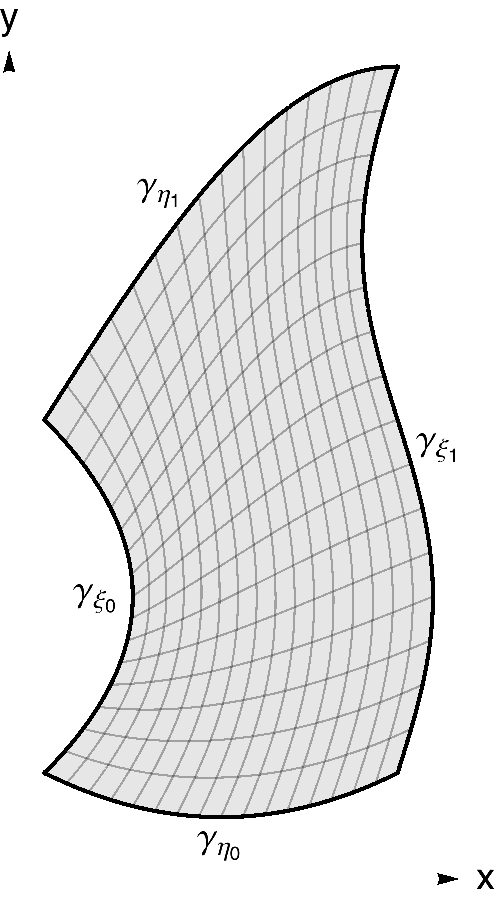
\includegraphics[width=.35\textwidth]{fig/testfig1.pdf}}

%=== Appendix ============================================
% \appendix
% \dsp
% % \chapter{Appendix}{\label{appendix:a}}
% \begin{section}{Datalog Program for Aggregation Events}

% \subsection{Moving window with {\sc count} function}

% Let \texttt{Src} be the source event and $L+1$ the window size for a moving rule
% with the {\sc count} function,
% i.e., the rule has the form of Fig.\:\ref{fig:moving-count-rule}.

% \begin{figure}[h!]
% \begin{tabular}{ll}
% \texttt{resultMovingCount}$(\mbox{\sc count}(a),s)@(s+L) \leftarrow$    & $\textsc{Over}\ {\sc Moving}(s,s+L)$\\
%                                                                             & $\textsc{From}\ \mbox{\tt Src}(a)@x$
% \end{tabular}\\
% \caption{Rule for moving window with {\sc count} function}
% \label{fig:moving-count-rule}
% \end{figure}

% To compute \texttt{resultMovingCount} incrementally,
% we use an internal event \texttt{incMovingCount}
% with attributes {\em accumulator},
% {\em start},
% {\em end},
% and {\em stop}.
% The {\em start} attribute is the window's first timestamp.
% The {\em accumulator} attribute
% holds the count seen from {\em start} to the timestamp {\em stop},
% where {\em stop} is the latest timestamp for the window seen thus far
% and used as each \texttt{incMovingCount} event's timestamp.
% The {\em end} attribute is the window's last timestamp
% and indicates when the result should be reported.\\

% We use a Datalog program (Fig.\:\ref{fig:moving-count-infty})
% to generate \texttt{incMovingCount} events as follows:
% each timestamp is the start of a moving window
% so for each source event at timestamp $T$,
% an \texttt{incMovingCount} event is initialized
% using a source event's timestamp as the window start,
% a $1$ in the accumulator if a ``genuine'' source event is present,
% i.e., if the source event value is not $-\infty$,
% otherwise a $0$,
% and $T{+}L$ as the window end.
% Data in \texttt{incMovingCount} at a timestamp $T$ is propagated
% to the next timestamp $T{+}1$ using the source event at timestamp $T{+}1$.
% To do this, the accumulator is incremented if the source event is real,
% and unchanged otherwise.
% The propagation only happens if the next timestamp is no greater than the window end.
% When the source timestamp is equal to the window end,
% the value in the accumulator is reported with \texttt{resultMovingCount}.\\

% \begin{figure}[h!]
% \begin{mdframed}[leftmargin=0pt,rightmargin=0mm]
% \begin{small}
% \begin{tabular}{ll}
% \multicolumn{2}{l}{Initialize \texttt{incMovingCount}}\\
% \texttt{incMovingCount}$(0, T, T{+}L)@T$ & $\leftarrow \mbox{\tt Src}(V,0)@T$\\
% \texttt{incMovingCount}$(1, T, T{+}L)@T$ & $\leftarrow \mbox{\tt Src}(V,1)@T$\\
% & \\
% \multicolumn{2}{l}{Propagate \texttt{incMovingCount}}\\
% \texttt{incMovingCount}$(A, S, E)@(T{+}1)$ & $\leftarrow$ \texttt{incMovingCount}$(A, S, E)@T ,\  \mbox{\tt Src}(V,0)@(T{+}1),\ (T{+}1{\leq}E)$\\
% \texttt{incMovingCount}$(A{+}1, S, E)@(T{+}1)$ & $\leftarrow$ \texttt{incMovingCount}$(A, S, E)@T ,\  \mbox{\tt Src}(V,1)@(T{+}1),\ (T{+}1{\leq}E)$\\
% & \\
% \multicolumn{2}{l}{Report \texttt{resultMovingCount}}\\
% \texttt{resultMovingCount}$(A, S, E)@T$ & $\leftarrow$ \texttt{incMovingCount}$(A, S, E)@T ,\  (T=E)$\\
% \end{tabular}
% \end{small}
% \end{mdframed}
% \caption{Datalog Program \texttt{incMovingCount} and \texttt{resultMovingCount}}
%     \label{fig:moving-count-infty}
% \end{figure}

% \subsection{Start-triggered window for {\sc max} function}

% Let \texttt{Src} be the source event,
% $L$ the window size,
% and \texttt{Start} a dataless start trigger event
% for a start-triggered rule with the {\sc max} function,
% i.e., the rule has the form of Fig.\:\ref{fig:start-trigger-max-rule}.

% \begin{figure}[h!]
% \begin{tabular}{ll}
% \texttt{resultStartTriggerMax}$(\mbox{\sc max}(a),s)@(s{+}L) \leftarrow$ & $\textsc{Over}({\tt Start}@s, s+L)$\\
%                             & $\textsc{From}\ \mbox{\tt Src}(a)@x$\\
% \end{tabular}
% \caption{Start-triggered rule with {\sc max} function}
% \label{fig:start-trigger-max-rule}
% \end{figure}

% We use a Datalog program (Fig.\:\ref{fig:start-trigger-max-program}) to generate
% \texttt{incStartTriggerMax} events as follows:
% Whenever a start trigger event is observed,
% an \texttt{incStartTriggerMax} event is initialized
% using the start trigger event's timestamp $T$ as the window start,
% the source event's value in the {\em accumulator},
% and $T{+}L$ as the window end.
% Data in \texttt{incStartTriggerMax} at a timestamp $T$ is propagated to the next timestamp $T{+}1$ using the source event at timestamp $T{+}1$.
% To do this, if the source event is real,
% the accumulator is compared with the value of the source event
% at timestamp $T{+}1$ and the larger is passed along.
% If the source event is not real,
% the accumulator is passed along.
% The propagation only happens if the next timestamp is no greater than the window end.
% When the source timestamp is equal to the window end,
% the value in the accumulator is reported with \texttt{reportStartTriggerMax}.\\

% \begin{figure}[h!]
% \begin{mdframed}[leftmargin=0pt,rightmargin=0mm]
% \begin{small}
% \begin{tabular}{ll}
% \multicolumn{2}{l}{Initialize \texttt{incStartTriggerMax}}\\
% \texttt{incStartTriggerMax}$(V, T, T{+}L)@T$ & $\leftarrow \mbox{\tt Src}(V,1)@T,\ \texttt{Start}@(T)$\\
% \texttt{incStartTriggerMax}$(-\infty, T, T{+}L)@T$ & $\leftarrow \mbox{\tt Src}(V,0)@T,\ \texttt{Start}@(T)$\\
% & \\
% \multicolumn{2}{l}{Propagate \texttt{incStartTriggerMax}}\\
% \texttt{incStartTriggerMax}$(V, S, E)@(T{+}1)$ & $\leftarrow$ \texttt{incStartTriggerMax}$(A, S, E)@T ,\  \mbox{\tt Src}(V,1)@(T{+}1) ,\  (A{<} V),\ (T{+}1 {\leq} E)$\\
% \texttt{incStartTriggerMax}$(A, S, E)@(T{+}1)$ & $\leftarrow$ \texttt{incStartTriggerMax}$(A, S, E)@T ,\  \mbox{\tt Src}(V,1)@(T{+}1) ,\  (A{\geq}V),\ (T{+}1 {\leq} E)$\\
% \texttt{incStartTriggerMax}$(A, S, E)@(T{+}1)$ & $\leftarrow$ \texttt{incStartTriggerMax}$(A, S, E)@T ,\  \mbox{\tt Src}(V,0)@(T{+}1) ,\ (T{+}1 {\leq} E)$\\
% & \\
% \multicolumn{2}{l}{Report \texttt{resultStartTriggerMax}}\\
% \texttt{resultStartTriggerMax}$(A, S, E)@T$ & $\leftarrow$ \texttt{incStartTriggerMax}$(A, S, E)@T,\ (T{=}E)$\\
% \end{tabular}
% \end{small}
% \end{mdframed}
% \caption{Datalog Program \texttt{incStartTriggerMax} and \texttt{resultStartTriggerMax}}
%     \label{fig:start-trigger-max-program}
% \end{figure}

% \subsection{End-triggered window for {\sc max} function}\label{end-triggered-algorithm}

% Let \texttt{Src} be the source event,
% $L+1$ the window size,
% and \texttt{End} a dataless end trigger event
% for an end-triggered rule with the {\sc max} function,
% i.e., the rule has the form of Fig.\:\ref{fig:end-trigger-max-rule}.

% \begin{figure}[h!]
% \begin{tabular}{ll}
% \texttt{resultEndMax}$(\mbox{\sc max}(a),e-L,e)@e \leftarrow$ & $\textsc{Over}(e-L,\texttt{End}@e)$\\
%                             & $\textsc{From}\ \mbox{\tt Src}(a)@x$\\
% \end{tabular}
% \caption{Rule $r$ with the {\sc max} function, end-triggered window $[e-L,e]$}
% \label{fig:end-trigger-max-rule}
% \end{figure}

% We use a Datalog program (Fig.\:\ref{fig:end-trigger-max})
% to generate \texttt{incEndMax} events as follows:
% each timestamp is possibly the start of an end-triggered window
% so for each source event at timestamp $T$,
% an \texttt{incEndMax} event is initialized
% using a source event's timestamp as the window start,
% the source event's value in the accumulator,
% and $T{+}L$ as the window end.
% Data in \texttt{incEndMax} at a timestamp $T$ is propagated to the next timestamp $T{+}1$ using the source event at timestamp $T{+}1$.
% To do this, if the source event is real,
% the accumulator is compared with the value of the source event
% at timestamp $T{+}1$ and the larger is passed along.
% If the source event is not real,
% the accumulator is passed along.
% The propagation only happens if the next timestamp is no greater than the window end.
% We report the value of the accumulator with \texttt{resultEndMax}
% when window's end stored in \texttt{incEndMax} coincides
% with an \texttt{End} event.\\

% \begin{figure}[h!]
% \begin{mdframed}[leftmargin=0pt,rightmargin=0mm]
% \begin{small}
% \begin{tabular}{ll}
% \multicolumn{2}{l}{Initialize \texttt{incEndMax}}\\
% \texttt{incEndMax}$(V, T, T{+}L)@T$ & $\leftarrow \mbox{\tt Src}(V,1)@T$\\
% \texttt{incEndMax}$(-\infty, T, T{+}L)@T$ & $\leftarrow \mbox{\tt Src}(V,0)@T$\\
% & \\
% \multicolumn{2}{l}{Propagate \texttt{incEndMax}}\\
% \texttt{incEndMax}$(V, S, E)@(T{+}1)$ & $\leftarrow$ \texttt{incEndMax}$(A, S, E)@T ,\  \mbox{\tt Src}(V)@(T{+}1) ,\  (A{<}   V),\ (T{+}1 {\leq} E)$\\
% \texttt{incEndMax}$(A, S, E)@(T{+}1)$ & $\leftarrow$ \texttt{incEndMax}$(A, S, E)@T ,\  \mbox{\tt Src}(V)@(T{+}1) ,\  (A{\geq}V),\ (T{+}1 {\leq} E)$\\
% & \\
% \multicolumn{2}{l}{Report \texttt{resultEndMax}}\\
% \texttt{resultEndMax}$(A, S, E)@T$ & $\leftarrow$ \texttt{incEndMax}$(A, S, E)@T ,\  (T{=}E),\ \texttt{End}@T$\\
% \end{tabular}
% \end{small}
% \end{mdframed}
% \caption{Datalog program for \texttt{incEndMax} and \texttt{resultEndMax}}
%     \label{fig:end-trigger-max}
% \end{figure}

% \end{section}
\end{mainmatter}

%----- Bibliography ----------------
\ssp
\bibliographystyle{JHEP3}
\bibliography{bibliography}

\end{document}